% Gelfand seminar notes, 1965-66: source pages P000088-P000139.
% English translation (AI-made, checked against the scans), cut page by page from the cumulative working reader A4-reader-chapters01-19-first973-separated-diplomatic-r1.
% \SourcePage{GELFAND-Pnnnnnn}{label} starts a scanned page; the second argument is the number written
% on the page, if any. Editorial notes give the page, a label and the transcriber's remark; \Unclear
% marks a doubtful reading.
\SourcePage{GELFAND-P000088}{unlabelled}
\underline{Unsolved problems.} (and solved ones)
\SourceFigure{GELFAND-P000088}{heading-marks}{“Unsolved problems.” is underlined; the parentheses are outside the underline. Below, “Conjecture.” is separately underlined.}
$p$ — entire fn., $p(A)$ — comp., then triv. $\exists M$
(use for polynomials).
de Branges — Rovnyak announced $\forall$ cont. oper.,
but with an error in the proof.
From their reasoning follows:
\begin{equation*}
\|A\|<1,\quad1-A^*A\ \text{comp.}\quad\Rightarrow\quad
\exists\text{ inv. subsp.}
\end{equation*}
\SourceFigure{GELFAND-P000088}{first-implication}{The first sign is $<$; then $1-A^*A$ and a double arrow to $\exists$.}
Res. of Sakhnovich, Livshits and brodsky.
$A+iB$, $A$ — self-adj., $B$ in some sense small (nuclear, etc.).
\SourceFigure{GELFAND-P000088}{selfadjoint-small}{At the start $A+iB$; “nuclear, etc.” continues on the second line.}
Nagy —
Foias / Foas
\Unclear{GELFAND-P000088}{foas-name}{Foias / Foas}
\begin{gather*}
\|A\|\leq1,\qquad A^n\mathrel{\not\longrightarrow}0\quad(\text{strongly}),\\
A^{*n}\mathrel{\not\longrightarrow}0
\end{gather*}
$\Rightarrow\exists$ inv. subsp.
\Unclear{GELFAND-P000088}{nonconvergence}{Both arrows are crossed by an inclined stroke.}
Triv. structure $\{0,1\}$.
\SourceFigure{GELFAND-P000088}{trivial-structure}{Two elements $\{0,1\}$; then the question about an operator in Hilb. sp. and “Not solved.”}
$\exists$ an oper. in Hilb. sp. with such a struct. of inv. subsp.? Not solved.
Another probl. Struct. $\{0,1,2,\ldots,\infty\}$.
Does an oper. with such a struct. exist?
Affirm. answer Donoghue (1957).
\SourceFigure{GELFAND-P000088}{countable-structure}{Written $\{0,1,2,\ldots,\infty\}$; the date in parentheses $(1957)$.}
\begin{center}
\begin{tikzpicture}[x=1.25mm,y=1.25mm,baseline=(current bounding box.center)]
\draw[line width=.6pt] (0,20) .. controls (-3,14) and (-3,4) .. (0,0);
\draw[line width=.6pt] (34,19) .. controls (38,13) and (38,4) .. (34,-2);
\node at (5.5,18) {$0$};
\node at (10.5,19.5) {$\frac12$};
\node at (11.5,13.2) {$0$};
\node at (17,15) {$\frac14$};
\node[font=\Large] at (6,7) {$0$};
\node at (17,8) {$\cdot$};
\node at (24,8) {$\frac18\,{\color{orange}[?]}$};
\node at (28,4) {$\cdot$};
\node at (30,0) {$\cdot$};
\end{tikzpicture}
\end{center}
\SourceFigure{GELFAND-P000088}{donoghue-matrix}{Within round parentheses two small $0$s, $1/2$, $1/4$; the third densely overwritten coefficient $1/8$ / $1/6$; a large $0$ below and separate dots down to the right.}
Exact cond. on the numbers above the diag. are unknown (so that precisely these occur).
$\exists$ an oper. with the struct. of all integers $\to$ unknown.
\SourceFigure{GELFAND-P000088}{all-integers}{“all integers”; then an arrow and “unknown”.}
\begin{center}
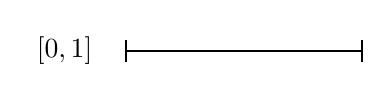
\begin{tikzpicture}[baseline=(current bounding box.center)]
\node[anchor=east] at (-.3,0) {$[0,1]$};
\draw[thick] (0,0)--(3,0);
\draw[thick] (0,-.14)--(0,.14);
\draw[thick] (3,-.14)--(3,.14);
\end{tikzpicture}
\end{center}
— such a structure $\exists$ operator.
\SourceFigure{GELFAND-P000088}{unit-interval}{On the left the label $[0,1]$, then a segment with two end strokes. Below $(Vf)(x)=\int_0^x f(y)\,dy$.}
\begin{equation*}
(Vf)(x)=\int_0^x f(y)\,dy
\end{equation*}
(answ. in the 1950s).
\underline{Conjecture.} A measure on the line $\mu$.
\begin{center}
\begin{tikzpicture}
\draw (0,0)--(4,0);
\node[below] at (0,0){$-\infty$};
\node[below] at (4,0){$+\infty$};
\end{tikzpicture}
\SourceFigure{GELFAND-P000088}{measure-line}{Below the line $-\infty$ on the left, $+\infty$ on the right.}
\end{center}
\begin{equation*}
\mu(x)=1,\qquad L^2(\mu).
\end{equation*}
[Above the first argument: $(x)$.]
\Unclear{GELFAND-P000088}{measure-normalization}{Visible $\mu(x)=1$ and another $(x)$ above; $\mu$ / $M$. Below the first letter a separate short mark: $2$ / illegible sign.}
\begin{equation*}
(Af)(x)=\int_0^x f(y)\,d\mu(y).
\end{equation*}
\Unclear{GELFAND-P000088}{integral-origin}{The lower limit is visible as $0$.}
Possibly, the struct. of inv. subsp. is isomorphic to $\operatorname{supp}\mu$.
\Unclear{GELFAND-P000088}{support-letter}{In $L^2(\mu)$ and after $\operatorname{supp}$ the letter $\mu$ / $M$.}


\Needspace{5\baselineskip}
\SourcePage{GELFAND-P000089}{61}
\underline{Possible counterexample.}
$X$ — sp. with measure $\mu$.
$T$ — transf., preserving measure (in Russian a dyn. system).
$\varphi$ — bounded fn.
[Crossed out before the formula:
Oper. / illegible.]
\Unclear{GELFAND-P000089}{operator-cancel}{Oper. / illegible}
[Above the formula: in $L^2$.]
\begin{equation*}
(Af)(x)=\varphi(x)f(Tx).
\end{equation*}
\SourceFigure{GELFAND-P000089}{weighted-formula}{Above $X,T,\varphi$; above the formula “in $L^2$”; on the right $f(Tx)$.}
$\exists$ examples of transf. with simple cont. spectrum.
\begin{center}
\begin{tikzpicture}
\draw (0,0)--(3,0);
\draw (0,-0.12)--(0,0.12);
\draw (3,-0.12)--(3,0.12);
\node[below] at (0,0){$0$};
\node[below] at (3,0){$1$};
\end{tikzpicture}
\end{center}
\begin{gather*}
Tx=x+\alpha\pmod1,\qquad\alpha\text{ — irr.}\\
\varphi(x)=x.
\end{gather*}
\SourceFigure{GELFAND-P000089}{interval-rotation}{A segment with two end strokes, labels $0$, $1$ below. On the right $Tx=x+\alpha\pmod1$, “$\alpha$ — irr.”, then $\varphi(x)=x$.}
\begin{quote}
\begin{tabular}{||l}
Study in detail\\
\uwave{this operator}
\end{tabular}
\end{quote}
\SourceFigure{GELFAND-P000089}{study-emphasis}{In the right margin two vertical strokes; a wavy line below “this operator”.}
Conjecture:
[Crossed out:
on one… / on a giv… (“на один…” / “на дан…”) / illegible.]

no inv. subsp. ($\forall$ vector cyclic).
\Unclear{GELFAND-P000089}{conjecture-cancel}{on one… / on a giv… (“на один…” / “на дан…”) / illegible}
In fact, not a single cyclic vector is known.
\SourceFigure{GELFAND-P000089}{cyclic-assertions}{In parentheses $\forall$ vector cyclic; below “not a single cyclic vector is known”.}
$\exists$ an example of an oper. $A$ in $L^2(0,1)$ (Ornstein), close to
an oper. without inv. subsp.
$\forall$ vector $\in L^{2+\varepsilon}$ cyclic (!).
\SourceFigure{GELFAND-P000089}{Ornstein}{In the first line $L^2(0,1)$ and the name Ornstein; below $\forall$, $\in L^{2+\varepsilon}$ and $(!)$.}
(A transf. for which Lebesgue measure is quasi-inv. — measure $0$ to measure $0$ —
but an inv. measure does not exist.)
\SourceFigure{GELFAND-P000089}{quasi-invariance}{“measure $0$ to measure $0$”; after the line break “but an inv. measure does not exist”.}
\begin{center}— $\bullet$ —\end{center}
\underline{Gelfand's question}: why are inv. subsp. needed, and what can replace them?
\SourceFigure{GELFAND-P000089}{Gelfand-question}{“Gelfand's question” is underlined; before and after the question, separators with a dot between two lines.}
\begin{center}— $\bullet$ —\end{center}
Another professor, speaking English (beginning with F)
(a Hungarian from Romania), something like
Foytsh / Foyshi (“Фойтш” / “Фойши”)
\Unclear{GELFAND-P000089}{surname-f}{Foytsh / Foyshi (“Фойтш” / “Фойши”)}
[A repeated entry is densely overwritten:
oyshi / Foyshi (“ойши” / “Фойши”) / illegible.]
\Unclear{GELFAND-P000089}{surname-cancel}{oyshi / Foyshi (“ойши” / “Фойши”) / illegible}
\begin{gather*}
E,\qquad|\lambda|<1,\qquad \mathord{\tikz[baseline=(h.base)]{\node[draw,circle,inner sep=.7pt] (h) {$H$};}}(\lambda):E\longrightarrow E_*,\\
\|H(\lambda)\|\leq1.
\end{gather*}
\SourceFigure{GELFAND-P000089}{contraction-math}{Separately $E$; $|\lambda|<1$; the first letter $H$ is circled, the right $E$ has a lower star; below $\|H(\lambda)\|\leq1$.}
[The letter $H$ in the first entry is circled.]
Analyt. in the strong oper. top. (analyt. contraction).
\begin{equation*}
\{E,E_*,\mathord{\tikz[baseline=(h.base)]{\node[draw,circle,inner sep=.7pt] (h) {$H$};}}\}
\end{equation*}
[The last letter in the triple is circled.]
\Unclear{GELFAND-P000089}{tuple-letter}{The circled sign in the triple: $H$ / $\Theta$ / illegible; above, the circled $H$ has two clear upright strokes.}
Sp. of fns. with values in the initial Hilb. sp. $E$.
$L^2(E)$ — $L^2$ on the circ. $2\pi$.
\SourceFigure{GELFAND-P000089}{Hardy-space}{In the upper line Hilb. sp. $E$; then $L^2(E)$, $2\pi$ and $H^2(E)$; the exponent has $+int$.}
\begin{equation*}
H^2(E)\qquad\int_0 u(t)e^{int}\,dt=0,\qquad n=1,2,3,\ldots
\end{equation*}
\Unclear{GELFAND-P000089}{fourier-bound}{The integral clearly has a lower $0$; no separate upper limit is visible.}
(boundary values of analyt. fns.).
Not everything has been done in the non-finite-dimensional case.
Inv. aff. transf. $A:H_1\longrightarrow H_2$,
\Unclear{GELFAND-P000089}{last-invariants}{The abbreviation aff. / diff. (“афф.” / “дифф.”); below $H\to H$ and “Jordan form”.}
$H_1,H_2$ — finite-dimensional.
($H\to H$ — Jordan form.)
Various analogues of Jordan blocks.
\begin{equation*}
\int_0^x f(x)\,dx.
\end{equation*}
\SourceFigure{GELFAND-P000089}{final-integral}{Upper limit $x$, lower $0$; the integrand and the differential also have $x$.}


\Needspace{5\baselineskip}
\SourcePage{GELFAND-P000090}{unlabelled}
$20/\overline{\underline{\mathrm{IX}}}$.
\underline{Kohn.}\quad $\bar\partial$ — Neumann probl.
\begin{center}
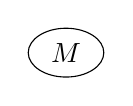
\begin{tikzpicture}
\node (m) at (0,0) {$M$};
\draw (0,0) ellipse (.48cm and .31cm);
\end{tikzpicture}
\end{center}
\SourceFigure{GELFAND-P000090}{opening-marks}{Date $20/\mathrm{IX}$: strokes above and below $\mathrm{IX}$; Kohn underlined; on the left $M$ in an oval.}
\begin{equation*}
M\subset C^n\qquad\text{bounded dom.}
\end{equation*}
\Unclear{GELFAND-P000090}{complex-dimension}{The exponent above $C$ is dense: $n$ / $m$.}
\begin{equation*}
u_{\bar z_j}=\frac12(u_{x_j}+iu_{y_j})=\alpha_j.
\end{equation*}
\SourceFigure{GELFAND-P000090}{first-derivative}{In the first definition a bar above $z_j$; on the right $\frac12$, the sign $+$ and $i$, then $\alpha_j$.}
Given $\alpha_j$, when does $\exists u$ and how does it depend on $\alpha$.
Connection with class. theorems.
\begin{gather*}
\bar\partial u=\alpha,\\
\sum u_{z_j}\,d\bar z_j=\sum\alpha_j\,d\bar z_j\\
\text{under cond. }\alpha_{j\bar z_k}=\alpha_{k\bar z_j}\qquad(\bar\partial\alpha=0).
\end{gather*}
\SourceFigure{GELFAND-P000090}{compatibility}{Bars above $z_j$ in the differentials; condition $\alpha_{j\bar z_k}=\alpha_{k\bar z_j}$, on the right $(\bar\partial\alpha=0)$.}
\Unclear{GELFAND-P000090}{derivative-convention}{In the sum the subscript $z_j$ has no confidently visible bar; above, in the definition, $\bar z_j$ is clear.}
\underline{Levi problem.}
\SourceFigure{GELFAND-P000090}{Levi-heading}{The heading has a straight underline; in the question $p$, $M$, the sign $\exists$ and abbreviations.}
Given $p\in\partial M$ (bound.),
[Crossed out:
which (“какая”) / illegible.]

$\exists$ a holom. fn. in $M$, which does not continue beyond the point $p$? Exists.
\Unclear{GELFAND-P000090}{levi-problem-cancel}{which (“какая”) / illegible}
\uwave{The class. Levi theor. solves this probl. locally:}
\SourceFigure{GELFAND-P000090}{Levi-emphasis}{A wavy line under the whole sentence from “The class.” to “locally:”.}
$\underset{\substack{x\\0}}{r}$ — equ. of the boundary.
\begin{center}
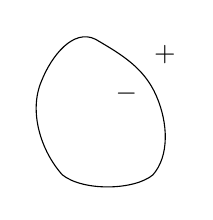
\begin{tikzpicture}[x=.014cm,y=-.014cm]
\draw (65,10) .. controls (45,0) and (25,25) .. (16,48)
 .. controls (4,76) and (16,112) .. (35,133)
 .. controls (54,148) and (100,147) .. (117,133)
 .. controls (132,116) and (131,86) .. (120,61)
 .. controls (109,36) and (89,24) .. (65,10) -- cycle;
\node at (93,59) {$-$};
\node at (128,24) {$+$};
\end{tikzpicture}
\end{center}
\SourceFigure{GELFAND-P000090}{boundary-signs}{An irregular closed curve, $-$ inside and $+$ outside above right. Below $r$ a small crossed sign resembling $x$, then $0$; their exact reading and role are not established.}
\begin{equation*}
\underline{dr\neq0}
\end{equation*}
\SourceFigure{GELFAND-P000090}{nonzero-differential}{The entry $dr\neq0$ has a straight underline; below “(point nonsingular)”.}
(point nonsingular).
At pt. $p\in\partial M$
\begin{equation*}
\sum r_{z_i}(p)a^i=0\qquad\text{hyperpl.}
\end{equation*}
\SourceFigure{GELFAND-P000090}{tangent-hyperplane}{Above the formula “At pt. $p\in\partial M$”; in the formula $a^i$ and $=0$; on the right “hyperpl.”.}
\begin{equation*}
\sum r_{z_i\bar z_j}(p)a^i\bar a^j
\end{equation*}
— Levi form.
\Unclear{GELFAND-P000090}{boundary-notation}{The boundary function's letter resembles $r$ / $\tau$, the boundary sign $\partial$ / $b$.}
If it is pos. def. on the indicated hyperplane,

then there exists in a neighb. of pt. $p$
[Crossed out:
illegible.]

a fn., not cont. beyond the point $p$.
\Unclear{GELFAND-P000090}{local-cancel}{illegible}
\SourceFigure{GELFAND-P000090}{Levi-positive}{Abbreviations “pos. def.”, “on the indicated hyperplane”, then “exists in a neighb. of pt. $p$”.}
($\exists$ a polynomial $W$, such that the zeros are arranged thus:
\begin{center}
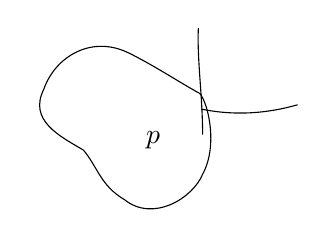
\begin{tikzpicture}[x=.018cm,y=-.018cm]
\draw (73,18) .. controls (46,4) and (20,20) .. (12,43)
 .. controls (1,65) and (23,76) .. (40,86)
 .. controls (50,98) and (52,111) .. (69,121)
 .. controls (89,137) and (117,120) .. (124,103)
 .. controls (135,83) and (128,53) .. (122,46)
 .. controls (109,39) and (91,27) .. (73,18) -- cycle;
\draw (121,0) .. controls (120,22) and (124,48) .. (124,75);
\draw (123,57) .. controls (147,62) and (170,60) .. (191,54);
\node at (89,79) {$p$};
\end{tikzpicture}
\end{center}
)
\SourceFigure{GELFAND-P000090}{local-w-geometry}{An irregular closed curve; at the right edge a nearly vertical stroke and a stroke running out to the right. Label $p$ inside, left and below their junction. The exact position of the dense overlapping strokes is not established.}
A good answer to that probl. ($\bar\partial$) leads to a glob. sol. of the Levi probl.
Let the $\bar\partial$-probl. be solvable for the dom. $M$
($\forall\alpha$, $\bar\partial\alpha=0$, $\exists u$, $\bar\partial u=\alpha$).
Let
\begin{equation*}
g=\begin{cases}1&\text{in a neighb. of }p,\\0&\text{outside }U\end{cases}
\end{equation*}
— cut-off fn.
\SourceFigure{GELFAND-P000090}{cutoff-values}{The entry $g$ has a brace, $1$ “in a neighb. of $p$”, $0$ “outside $U$”; on the right “cut-off fn.”.}
Denote $\alpha=\bar\partial\left(\frac gW\right)$.
$W$ — the previously constr. polynomial.
$\alpha$ — smooth up to the boundary.
\SourceFigure{GELFAND-P000090}{cutoff-alpha}{On the left $\alpha=\bar\partial(g/W)$; on the right $W$ — the previously constr. polynomial; below “smooth up to the boundary”.}
\begin{center}
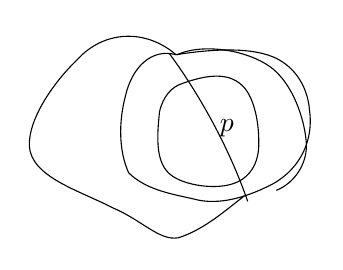
\begin{tikzpicture}[x=.014cm,y=-.014cm]
\draw (149,25) .. controls (121,1) and (83,3) .. (59,30)
 .. controls (40,48) and (15,82) .. (16,108)
 .. controls (18,136) and (61,148) .. (92,164)
 .. controls (118,175) and (134,194) .. (151,191)
 .. controls (174,184) and (194,166) .. (211,153);
\draw (150,25) .. controls (174,14) and (216,21) .. (237,38)
 .. controls (255,53) and (265,82) .. (267,103)
 .. controls (269,123) and (257,141) .. (240,148);
\draw (149,25) .. controls (127,19) and (109,36) .. (103,63)
 .. controls (97,86) and (97,112) .. (106,132)
 .. controls (123,149) and (150,152) .. (170,157)
 .. controls (192,161) and (216,153) .. (237,142)
 .. controls (262,128) and (274,102) .. (270,75)
 .. controls (268,51) and (254,34) .. (237,27)
 .. controls (213,17) and (174,21) .. (149,25) -- cycle;
\draw (155,51) .. controls (172,45) and (195,39) .. (209,53)
 .. controls (219,62) and (224,84) .. (224,103)
 .. controls (225,124) and (215,139) .. (197,143)
 .. controls (181,147) and (153,143) .. (142,132)
 .. controls (130,120) and (132,97) .. (134,77)
 .. controls (137,63) and (145,54) .. (155,51) -- cycle;
\draw (143,24) .. controls (168,58) and (196,106) .. (214,158);
\node at (195,92) {$p$};
\end{tikzpicture}
\end{center}
\SourceFigure{GELFAND-P000090}{cutoff-geometry}{Three irregular nested contours and an inclined stroke; a gap at the lower right of the outer contour. $p$ inside the small contour. No labels $U$ or boundary are visible at the contours; dense intersections are not fully distinguishable.}
Solve the equ. someh., obtain $u$, consider $h=u-\frac gW$.
\Unclear{GELFAND-P000090}{solution-h}{After “equ.” the abbreviation “к-л.” (someh.); the second letter is dense, the exact reading is not fully established. Then $u$, $h=u-\frac gW$.}
$h$ holom. (since $\bar\partial=0$)
[A stroke crossed out:
arrow (“стрелка”) / illegible.]
\Unclear{GELFAND-P000090}{final-arrow-cancel}{arrow (“стрелка”) / illegible}
$u$ does not continue.
\Unclear{GELFAND-P000090}{noncontinuation-letter}{Before “does not continue” the letter $u$ is visible.}
Analogo / Analogously (“Аналого” / “Аналогично”)
is also possible, but there it continues beyond the point.
\Unclear{GELFAND-P000090}{analogo-word}{Analogo / Analogously (“Аналого” / “Аналогично”)}
\begin{center}
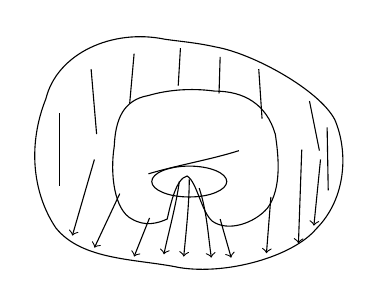
\begin{tikzpicture}[x=.014cm,y=-.014cm]
\draw (126,10) .. controls (78,0) and (28,23) .. (18,64)
 .. controls (2,104) and (5,148) .. (27,181)
 .. controls (51,211) and (101,209) .. (139,217)
 .. controls (182,224) and (242,207) .. (263,182)
 .. controls (291,154) and (292,111) .. (280,83)
 .. controls (266,56) and (206,23) .. (172,17)
 .. controls (154,13) and (140,12) .. (126,10) -- cycle;
\draw (111,61) .. controls (88,65) and (81,83) .. (80,107)
 .. controls (76,132) and (80,165) .. (96,173)
 .. controls (108,180) and (119,177) .. (128,173)
 .. controls (131,160) and (136,136) .. (146,134)
 .. controls (155,139) and (159,167) .. (169,175)
 .. controls (183,185) and (207,177) .. (219,163)
 .. controls (232,145) and (229,116) .. (226,96)
 .. controls (218,69) and (198,57) .. (171,57)
 .. controls (149,54) and (128,56) .. (111,61) -- cycle;
\draw (148,139) ellipse (34 and 14);
\draw (111,132) .. controls (138,124) and (168,119) .. (193,111);
\draw (30,77)--(30,143);
\draw (59,37)--(64,96);
\draw (98,23)--(94,68);
\draw (140,18)--(138,52);
\draw (176,26)--(175,59);
\draw (211,37)--(214,82);
\draw (257,66)--(266,111);
\draw (273,90)--(274,147);
\draw[->] (62,119)--(42,188);
\draw[->] (85,150)--(62,199);
\draw[->] (112,172)--(98,207);
\draw[->] (139,139) .. controls (136,161) and (129,186) .. (125,205);
\draw[->] (148,137) .. controls (148,159) and (145,186) .. (143,207);
\draw[->] (157,145) .. controls (164,166) and (165,187) .. (168,208);
\draw[->] (176,173)--(186,208);
\draw[->] (222,153)--(218,204);
\draw[->] (250,110)--(247,195);
\draw[->] (267,119)--(261,179);
\end{tikzpicture}
\end{center}
\SourceFigure{GELFAND-P000090}{global-geometry}{An outer contour; an inner contour with a lower notch; hatching between them. At the notch a small oval and an oblique stroke above it; several long strokes with downward arrows. Dense intersections and some stroke ends are not fully distinguishable.}
[Crossed out to the right of the drawing:
illegible.]
\Unclear{GELFAND-P000090}{figure-cancel}{illegible}
Must take into acc. the geom. structure of the entire domain as a whole.
\SourceFigure{GELFAND-P000090}{whole-domain}{The last sentence breaks to “domain.”; above “but there it continues beyond the point”.}


\Needspace{5\baselineskip}
\begin{GelfandAdjacentEvidence}{GELFAND-P000091}{1}
\SourcePage{GELFAND-P000091}{62}
$a^{p,q}$ — space of forms of type $p,q$.
\SourceFigure{GELFAND-P000091}{opening-type}{$a^{p,q}$; space of forms of type $p,q$.}
\end{GelfandAdjacentEvidence}
\begin{GelfandAdjacentEvidence}{GELFAND-P000091}{2}

\begin{equation*}
a^{p,q-1}\underset{\tikz[baseline=(e.base)]{\node[draw,ellipse,inner sep=1pt] (e) {$\text{eqn}$};}}{\overset{\bar\partial}{\longrightarrow}}
a^{p,q}\overset{\bar\partial}{\longrightarrow}\alpha^{p,q+1}.
\end{equation*}
\SourceFigure{GELFAND-P000091}{dolbeault-chain}{Two arrows with $\bar\partial$; under the first, eqn is enclosed in an oval.}
\Unclear{GELFAND-P000091}{forms-space-letter}{The initial and middle letters have the form $a$; the last in the chain and the following notation have the form $\alpha$. The local $a/\alpha$ variation is retained.}
\end{GelfandAdjacentEvidence}
\begin{GelfandAdjacentEvidence}{GELFAND-P000091}{3}

General theorems. $\alpha^{p,q}$ — Hilb. scalar product.
$\varphi,\psi\in D_{\bar\partial^*}$.
\begin{equation*}
Q(\varphi,\psi)=(\bar\partial\varphi,\bar\partial\psi)
+(\bar\partial^*\varphi,\bar\partial^*\psi).
\end{equation*}
[At the right:] ($\bar\partial$ on smooth forms of 1st degree without boundary conditions).
\SourceFigure{GELFAND-P000091}{Q-form}{$D_{\bar\partial^*}$, two terms in $Q(\varphi,\psi)$; at the right, parentheses about smooth forms of 1st degree without boundary conditions.}
\end{GelfandAdjacentEvidence}
\begin{GelfandAdjacentEvidence}{GELFAND-P000091}{4}

\begin{center}
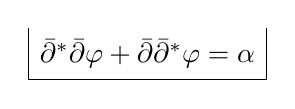
\begin{tikzpicture}
\node[inner sep=4pt] (op) {$\bar\partial^*\bar\partial\varphi+\bar\partial\bar\partial^*\varphi=\alpha$};
\draw (op.north west)--(op.south west)--(op.south east)--(op.north east);
\end{tikzpicture}
\end{center}
\SourceFigure{GELFAND-P000091}{boxed-operator}{Equation with two terms and right side $\alpha$; frame at the left, bottom and right, with no top side.}
\end{GelfandAdjacentEvidence}
\begin{GelfandAdjacentEvidence}{GELFAND-P000091}{5}

With the aid of a pos. def. prob. [Crossed out: illegible] of higher order solve a prob. of 1st order.
\Unclear{GELFAND-P000091}{positive-problem-cancel}{After prob., a former short expression is densely crossed out; an initial 1-/4-like stroke, the rest illegible.}
\end{GelfandAdjacentEvidence}
\begin{GelfandAdjacentEvidence}{GELFAND-P000091}{6}

But here it is used that the syst. is of 1st order and the solvability cond. is of 1st order.
(On gen. overdet. syst. $\exists$ work of Spencer.)
Connection with the Neumann prob.
\SourceFigure{GELFAND-P000091}{first-order-argument}{Syst. of 1st order, solvability cond. of 1st order; in parentheses $\exists$ work of Spencer; then connection with the Neumann prob.}
\end{GelfandAdjacentEvidence}
\begin{GelfandAdjacentEvidence}{GELFAND-P000091}{7}

A priori est.
\begin{equation*}
\int_{\partial M}|\varphi|^2\,dS\le C Q(\varphi,\varphi)
\qquad\forall\varphi\in D_{\bar\partial^*}\cap\alpha^{p,q}.
\end{equation*}
\SourceFigure{GELFAND-P000091}{apriori-estimate}{The integral has $\partial M$, integrand $|\varphi|^2dS$; $\le C Q(\varphi,\varphi)$ and $\forall\varphi\in D_{\bar\partial^*}\cap\alpha^{p,q}$.}
\end{GelfandAdjacentEvidence}
\begin{GelfandAdjacentEvidence}{GELFAND-P000091}{8}

(but not min. $\sum$ of squares of 1st derivs., $n=1\sim\int$ Dirichlet).
\SourceFigure{GELFAND-P000091}{Dirichlet-comparison}{Before $\sum$, min.; then squares of 1st derivs., $n=1\sim\int$ Dirichlet.}
\end{GelfandAdjacentEvidence}
\begin{GelfandAdjacentEvidence}{GELFAND-P000091}{9}

Attempt to apply projection (loc.) no, led nowhere.
(Cohn spent 2 years on this, $\int$ eqns and so on.)
Simplest case of the Neumann problem.
Cohn and Rossi Ann. Math. 1965 on holom. continuation of forms (!) into the domain.
\SourceFigure{GELFAND-P000091}{projection-and-Cohn}{Attempt to apply projection (loc.); Cohn in two places; 2 years, $\int$ eqns; Rossi, Ann. Math. 1965; $(!)$ after forms.}
\end{GelfandAdjacentEvidence}
\begin{GelfandAdjacentEvidence}{GELFAND-P000091}{10}


\uwave{Plans for the future}.
\SourceFigure{GELFAND-P000091}{plans-emphasis}{Wavy line beneath the heading Plans for the future.}
\Unclear{GELFAND-P000091}{plans-title-correction}{The word for in the heading is densely overwritten; the earlier strokes are illegible.}
\end{GelfandAdjacentEvidence}
\begin{GelfandAdjacentEvidence}{GELFAND-P000091}{11}

\underline{Study:} Vinberg (algebraic groups),
\SourceFigure{GELFAND-P000091}{study-heading}{Study: has a straight underline; Vinberg (algebraic groups).}
\end{GelfandAdjacentEvidence}
\begin{GelfandAdjacentEvidence}{GELFAND-P000091}{12}

Atiy[?] (…detail[?]; the beginning in parentheses is densely overwritten), alg. geometry.

\Unclear{GELFAND-P000091}{atiyah-parenthesis}{Atiy[?] (…detail[?]; the beginning in parentheses is densely overwritten), alg. geometry.}
\end{GelfandAdjacentEvidence}
\begin{GelfandAdjacentEvidence}{GELFAND-P000091}{13}

read for basic instruction:
[Crossed out:
Latin $G$… / Cyrillic Г…; the rest of the name is illegible.
] and Rossi “functions of several complex variables” 1965
(sheaves, cohom. and so on).
\Unclear{GELFAND-P000091}{cancelled-book-name}{Latin $G$… / Cyrillic Г…; the rest of the name is illegible.}
\SourceFigure{GELFAND-P000091}{reading-list}{After the cancelled name, and Rossi; functions of several complex variables, 1965; in parentheses, sheaves, cohom. and so on.}
\end{GelfandAdjacentEvidence}
\begin{GelfandAdjacentEvidence}{GELFAND-P000091}{14}

Review by Dieudonné of the work of Grothendieck
(Man. / Mat.[?] 9:1); the abbreviated first word is not entirely certain.

\Unclear{GELFAND-P000091}{review-volume}{(Man. / Mat.[?] 9:1); the abbreviated first word is not entirely certain.}
\end{GelfandAdjacentEvidence}
\begin{GelfandAdjacentEvidence}{GELFAND-P000091}{15}


$\underline{27/\overline{\underline{\mathrm{IX}}}}$ \underline{Finn}. Ideas in the Gauss--Bonnet theor.
\SourceFigure{GELFAND-P000091}{Finn-heading}{Separate straight lines under the date and Finn; short bars above and below IX.}
\end{GelfandAdjacentEvidence}
\begin{GelfandAdjacentEvidence}{GELFAND-P000091}{16}

Generalization of Cohn--Vossen: the surf. is not closed, but complete (e.g., a paraboloid).
\SourceFigure{GELFAND-P000091}{Finn-surface-statement}{The surf. is not closed, but complete; in parentheses, e.g., a paraboloid.}
\end{GelfandAdjacentEvidence}
\begin{GelfandAdjacentEvidence}{GELFAND-P000091}{17}

$C=2\pi$ [Crossed-out sign: illegible]; $\chi=1$.
\Unclear{GELFAND-P000091}{finn-curvature-cancel}{After the first $C=2\pi$ a sign is densely crossed out; its exact reading is not established.}
\end{GelfandAdjacentEvidence}
\begin{GelfandAdjacentEvidence}{GELFAND-P000091}{18}

\begin{center}
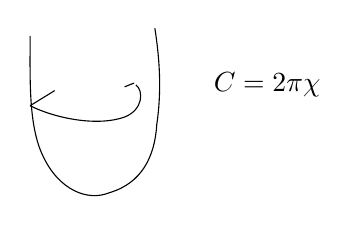
\begin{tikzpicture}[x=.024cm,y=-.024cm]
\draw (10,20) .. controls (10,43) and (9,68) .. (17,84)
 .. controls (25,101) and (40,108) .. (52,103)
 .. controls (69,98) and (76,84) .. (77,67)
 .. controls (80,47) and (78,29) .. (76,16);
\draw (10,57) .. controls (24,64) and (46,68) .. (60,63)
 .. controls (70,59) and (70,49) .. (66,46);
\draw (10,57)--(23,49);
\draw (60,47)--(65,45);
\node[anchor=west] at (102,46) {$C=2\pi\chi$};
\end{tikzpicture}
\qquad
\begin{tikzpicture}[x=.024cm,y=-.024cm]
\draw (0,0) .. controls (6,20) and (15,38) .. (30,49)
 .. controls (45,60) and (67,65) .. (88,63)
 .. controls (114,61) and (130,47) .. (138,29)
 .. controls (145,14) and (147,1) .. (146,-5);
\node[anchor=west] at (173,25) {$\chi=1$};
\node[anchor=west] at (135,93) {for it $C<2\pi$};
\end{tikzpicture}
\end{center}
\SourceFigure{GELFAND-P000091}{finn-sections}{Two lines opening upward; the small one at the left has a short curved transverse stroke with thickened ends. Its exact role and direction are not established. To its right $C=2\pi\chi$; by the large one $\chi=1$, below, for it $C<2\pi$.}
\end{GelfandAdjacentEvidence}
\begin{GelfandAdjacentEvidence}{GELFAND-P000091}{19}

($C=\int K\,dS$).
\SourceFigure{GELFAND-P000091}{curvature-integral}{$C=\int KdS$ is enclosed in round parentheses.}
\end{GelfandAdjacentEvidence}
\begin{GelfandAdjacentEvidence}{GELFAND-P000091}{20}

Cohn--Vossen theor.: $\forall$ complete surf. $C\le2\pi\chi$.
\SourceFigure{GELFAND-P000091}{Finn-final-bound}{The last line has $\forall$ complete surf. and $C\le2\pi\chi$.}
\end{GelfandAdjacentEvidence}




\begin{GelfandAdjacentEvidence}{GELFAND-P000092}{1}
\SourcePage{GELFAND-P000092}{unlabelled}
Aim of the work — to replace the inequality by an equality.
\SourceFigure{GELFAND-P000092}{opening-purpose}{Aim of the work — to replace the inequality by an equality.}
\end{GelfandAdjacentEvidence}
\begin{GelfandAdjacentEvidence}{GELFAND-P000092}{2}

Next time a review by
Volevich[?]

on var., anal. bundles.
\Unclear{GELFAND-P000092}{reviewer-name}{Volevich[?]}
\end{GelfandAdjacentEvidence}
\begin{GelfandAdjacentEvidence}{GELFAND-P000092}{3}

$Kohn$'om[?]

\Unclear{GELFAND-P000092}{next-review-name}{$Kohn$'om[?]; dense beginning of the name and ending after the apostrophe.}
\end{GelfandAdjacentEvidence}
\begin{GelfandAdjacentEvidence}{GELFAND-P000092}{4}


\underline{Gelfand.}
[Crossed out: Atiy…; ending illegible.] \underline{Atiyah.}

\Unclear{GELFAND-P000092}{atiyah-heading-cancel}{[Crossed out: Atiy…; ending illegible.] \underline{Atiyah.}}
\end{GelfandAdjacentEvidence}
\begin{GelfandAdjacentEvidence}{GELFAND-P000092}{5}

\uwave{Fixed-point theorems.}
\SourceFigure{GELFAND-P000092}{heading-emphasis}{Straight lines under Gelfand. and Atiyah.; wavy line under Fixed-point theorems.}
\end{GelfandAdjacentEvidence}
\begin{GelfandAdjacentEvidence}{GELFAND-P000092}{6}

(contains Brouwer's theor., the Lefschetz formula, the theor. that a lin. space has an eigenvector,
Weyl's theor. on traces of reps. and so on.)
\SourceFigure{GELFAND-P000092}{fixedpoint-examples}{At the beginning of the parentheses, contains; then Brouwer's theor., the Lefschetz formula, eigenvector, Weyl's theor. on traces of reps.}
\end{GelfandAdjacentEvidence}
\begin{GelfandAdjacentEvidence}{GELFAND-P000092}{7}

$X$ — diff. manifold and on it $n$ vector bundles $E_1,\ldots,E_n$.
$\Gamma(E_i)$ — sections of $E_i$. (each bundle — its own dim.)
\SourceFigure{GELFAND-P000092}{bundle-sections}{$X$, $n$, $E_1,\ldots,E_n$ and $\Gamma(E_i)$; in parentheses, each bundle — its own dim.; the last ending of the Russian word for its own is tight.}
\end{GelfandAdjacentEvidence}
\begin{GelfandAdjacentEvidence}{GELFAND-P000092}{8}

\underline{Example:} $X\times I$ ($I$ — a straight line). Space of functions.
\SourceFigure{GELFAND-P000092}{trivial-bundle}{Straight underline under Example:; $X\times I$, $I$ — a straight line, space of functions.}
\end{GelfandAdjacentEvidence}
\begin{GelfandAdjacentEvidence}{GELFAND-P000092}{9}

\uwave{Elliptic complex} (generalizes ell. diff. operators).
\SourceFigure{GELFAND-P000092}{elliptic-heading}{Wavy line under Elliptic complex; then generalizes ell. diff. operators.}
\end{GelfandAdjacentEvidence}
\begin{GelfandAdjacentEvidence}{GELFAND-P000092}{10}

\begin{equation*}
\Gamma(E_1)\overset d\longrightarrow\Gamma(E_2)\overset d\longrightarrow
\cdots\overset d\longrightarrow\Gamma(E_n).
\end{equation*}
a seq. of linear maps such that $1^\circ\ d^2=0$.
\SourceFigure{GELFAND-P000092}{differential-chain}{Three arrows with $d$; $\Gamma(E_1)$, $\Gamma(E_2)$, ellipsis, $\Gamma(E_n)$; $1^\circ$, $d^2=0$.}
\end{GelfandAdjacentEvidence}
\begin{GelfandAdjacentEvidence}{GELFAND-P000092}{11}

$2^\circ$. Consider $e\in E_{i,x_0}$, $s(x)\in\Gamma(E_i)$, such that $s(x_0)=e$.
Let $f(x)$ be a function taking the value $0$ at the point $x_0$.
Consider $d(f^m s(x))=s_1(x)\in\Gamma(E_{i+1})$.
\SourceFigure{GELFAND-P000092}{differential-condition}{$e\in E_{i,x_0}$; $s(x_0)=e$; function $f(x)$ vanishes at $x_0$; $d(f^m s(x))=s_1(x)\in\Gamma(E_{i+1})$.}
\end{GelfandAdjacentEvidence}
\begin{GelfandAdjacentEvidence}{GELFAND-P000092}{12}

Then, if
[Crossed out: $\exists$ with an illegible continuation.] $\exists m$,

such that $\forall x_0$ ($f(x_0)=0$) $s_1(x_0)$ depends only on the 1st differentials of $f$
at the point $x_0$, the operator is called differential.
($\exists m$ such that $\forall f$, $\forall x_0$, $\forall s$ and so on.)
The least $m$ is called the order of the diff. operator such that $s(x_0)=e$.
(In a neighbourhood of the point this is a local diff. operator.)
\Unclear{GELFAND-P000092}{m-condition-cancel}{[Crossed out: $\exists$ with an illegible continuation.] $\exists m$,}
\SourceFigure{GELFAND-P000092}{least-order}{Three $\forall$ signs in parentheses; the least $m$, then such that $s(x_0)=e$; in the final parentheses, in a neighbourhood of the point.}
\end{GelfandAdjacentEvidence}
\begin{GelfandAdjacentEvidence}{GELFAND-P000092}{13}

\begin{equation*}df=(\eta,dx).\end{equation*}
$df$ — [Short word crossed out: illegible] vector; $\eta$ — gradient (from [tang. inserted above densely overwritten strokes] space).

$\eta\in T_x^*$.
\Unclear{GELFAND-P000092}{gradient-corrections}{$df$ — [Short word crossed out: illegible] vector; $\eta$ — gradient (from [tang. inserted above densely overwritten strokes] space).}
\SourceFigure{GELFAND-P000092}{covector-source}{$df=(\eta,dx)$; alongside, $\eta$ — gradient; below, $\eta\in T_x^*$.}
\end{GelfandAdjacentEvidence}
\begin{GelfandAdjacentEvidence}{GELFAND-P000092}{14}

\begin{equation*}\sigma(d,\eta)e\end{equation*}

— a lin. function of $e$, called the symbol of the diff. operator.
\Unclear{GELFAND-P000092}{symbol-operator-cancel}{First argument: $d$ added above a densely cancelled sign; the former sign is illegible.}
\end{GelfandAdjacentEvidence}
\begin{GelfandAdjacentEvidence}{GELFAND-P000092}{15}

\underline{Example.} Laplace operator. $m=2$.
\begin{equation*}
\frac{\partial^2(f^2(x)s(x))}{\partial x^2}
=2\left(\frac{\partial f}{\partial x}\right)^2s(x).
\end{equation*}
\SourceFigure{GELFAND-P000092}{laplace-example}{Straight underline under Example.; $m=2$; $f^2(x)s(x)$ in the second derivative; on the right $2(\partial f/\partial x)^2s(x)$.}
\end{GelfandAdjacentEvidence}
\begin{GelfandAdjacentEvidence}{GELFAND-P000092}{16}

Symbol $2(\eta_1^2+\eta_2^2+\cdots+\eta_n^2)$.
\SourceFigure{GELFAND-P000092}{principal-symbol}{Factor $2$; $\eta_1^2+\eta_2^2+\cdots+\eta_n^2$.}
\end{GelfandAdjacentEvidence}
\begin{GelfandAdjacentEvidence}{GELFAND-P000092}{17}

Consider.
\begin{equation*}
0\longrightarrow E_{1,x_0}\overset{\sigma(\eta,d)}{\longrightarrow}E_{2,x_0}
\overset{\sigma(\eta,d)}{\longrightarrow}\cdots\longrightarrow E_{n,x_0}\longrightarrow0.
\end{equation*}
\SourceFigure{GELFAND-P000092}{symbol-sequence}{Zero endpoints; $E_{1,x_0}$, $E_{2,x_0}$, ellipsis, $E_{n,x_0}$; $\sigma(\eta,d)$ over the first two arrows.}
\end{GelfandAdjacentEvidence}
\begin{GelfandAdjacentEvidence}{GELFAND-P000092}{18}

The complex is elliptic if $\forall\eta\ne0$ this seq. is exact.
\SourceFigure{GELFAND-P000092}{elliptic-exactness}{The last line has $\forall\eta\ne0$ and this seq. is exact.}
\end{GelfandAdjacentEvidence}




\begin{GelfandAdjacentEvidence}{GELFAND-P000093}{1}
\SourcePage{GELFAND-P000093}{63}
\underline{Examples.} $1)$ $X$ — a domain in $R^n$.
sheaf $1$ ($X\times R$).
\SourceFigure{GELFAND-P000093}{opening-examples}{Straight underline under Examples.; $1)$, $X$, $R^n$, sheaf $1$, $X\times R$.}
\end{GelfandAdjacentEvidence}
\begin{GelfandAdjacentEvidence}{GELFAND-P000093}{2}

\begin{equation*}-\Gamma(1)\overset\Delta\longrightarrow\Gamma(1).\end{equation*}
Laplace operator.
\Unclear{GELFAND-P000093}{first-example-minus}{A short horizontal stroke before the first $\Gamma(1)$: minus / dash.}
\end{GelfandAdjacentEvidence}
\begin{GelfandAdjacentEvidence}{GELFAND-P000093}{3}

$2)$ de Rham complex.
\SourceFigure{GELFAND-P000093}{de-rham-heading}{$2)$ de Rham complex.}
\end{GelfandAdjacentEvidence}
\begin{GelfandAdjacentEvidence}{GELFAND-P000093}{4}

\begin{equation*}T^*\wedge T^*\wedge\cdots\wedge T^*=\Lambda^{k}\,[?].\end{equation*}
\Unclear{GELFAND-P000093}{exterior-power}{The $\Lambda$ itself is densely overwritten; small exponent $k$[?], also $n$- / $x$- / $\kappa$-like.}
\end{GelfandAdjacentEvidence}
\begin{GelfandAdjacentEvidence}{GELFAND-P000093}{5}

$T$ —
[Beginning of the word densely overwritten; former letters illegible] tang. space.

\Unclear{GELFAND-P000093}{tangent-word-cancel}{[Beginning of the word densely overwritten; former letters illegible] tang. space.}
\end{GelfandAdjacentEvidence}
\begin{GelfandAdjacentEvidence}{GELFAND-P000093}{6}

$X$ — manifold. $T_x$ — tang. space at the point $x$,
\SourceFigure{GELFAND-P000093}{tangent-space}{$X$ — manifold; $T_x$ — tang. space at the point $x$.}
\Unclear{GELFAND-P000093}{tangent-side-cancel}{[At the right: compact entry crossed out; T-/Phi-like strokes, exact reading undetermined.]}
\end{GelfandAdjacentEvidence}
\begin{GelfandAdjacentEvidence}{GELFAND-P000093}{7}

\begin{equation*}
\Gamma(\Lambda^0)\overset d\longrightarrow\Gamma(\Lambda^1)
\overset d\longrightarrow\cdots\overset d\longrightarrow\Gamma(\Lambda^n).
\end{equation*}
\Unclear{GELFAND-P000093}{de-rham-chain-cancels}{[Signs densely cancelled before the first $\Gamma(\Lambda^0)$, a separate short stroke at the left; after $\Gamma(\Lambda^n)$, an arrow and a $0$-like sign are crossed out.]}
\end{GelfandAdjacentEvidence}
\begin{GelfandAdjacentEvidence}{GELFAND-P000093}{8}

[At the right:] sections — \uwave{diff. forms.}
\SourceFigure{GELFAND-P000093}{sections-emphasis}{At the right, sections — diff. forms.; wavy line under diff. forms.}
\end{GelfandAdjacentEvidence}
\begin{GelfandAdjacentEvidence}{GELFAND-P000093}{9}

Symbol at the 1st step — $(\eta_1,\ldots,\eta_n)$.
\begin{equation*}
d(s(x)f(x))=s(x_0)\eta=e\eta\qquad(df(x_0)=\eta).
\end{equation*}
\SourceFigure{GELFAND-P000093}{first-symbol}{At the 1st step $(\eta_1,\ldots,\eta_n)$; $s(x_0)\eta=e\eta$; in parentheses $df(x_0)=\eta$.}
\end{GelfandAdjacentEvidence}
\begin{GelfandAdjacentEvidence}{GELFAND-P000093}{10}

In the 2nd place
\begin{equation*}
d(s(x)f(x))\big|_{x=x_0}
=s(x)\wedge df(x)\big|_{x=x_0}=e\wedge\eta.
\end{equation*}
\SourceFigure{GELFAND-P000093}{second-symbol}{Two restrictions $x=x_0$; $s(x)\wedge df(x)$ and $e\wedge\eta$.}
\end{GelfandAdjacentEvidence}
\begin{GelfandAdjacentEvidence}{GELFAND-P000093}{11}

(each subsequent symbol — multiplication by $\eta$).
\SourceFigure{GELFAND-P000093}{multiplication-statement}{Each subsequent symbol — multiplication by $\eta$, in parentheses.}
\end{GelfandAdjacentEvidence}
\begin{GelfandAdjacentEvidence}{GELFAND-P000093}{12}

\uwave{Exactness:} if $e\wedge\eta=0$, then $e=a\wedge\eta$.
\SourceFigure{GELFAND-P000093}{exactness-statement}{Wavy line under Exactness:; $e\wedge\eta=0$, $e=a\wedge\eta$.}
\end{GelfandAdjacentEvidence}
\begin{GelfandAdjacentEvidence}{GELFAND-P000093}{13}

(minors of the 2nd ord. $=0$, then the vectors [pryam.: meaning unclear]
[Final signs crossed out; dense entry, arrow and $0$-like ending; exact reading undetermined.]

)
\Unclear{GELFAND-P000093}{nilpotent-ending-cancel}{[Final signs crossed out; dense entry, arrow and $0$-like ending; exact reading undetermined.]}
\end{GelfandAdjacentEvidence}
\begin{GelfandAdjacentEvidence}{GELFAND-P000093}{14}

$3)$ $\bar\partial$ and so on.
\SourceFigure{GELFAND-P000093}{dolbeault-example}{$3)$; horizontal bar above $\partial$; and so on.}
\end{GelfandAdjacentEvidence}
\begin{GelfandAdjacentEvidence}{GELFAND-P000093}{15}


$4/\overline{\underline{\mathrm{X}}}$ \uuline{Continuation.} $\Gamma(E)$ — seq.
\SourceFigure{GELFAND-P000093}{continuation-date-heading}{Date $4/\overline{\underline{\mathrm{X}}}$; Continuation. underlined with two straight lines.}
\end{GelfandAdjacentEvidence}
\begin{GelfandAdjacentEvidence}{GELFAND-P000093}{16}

\begin{equation*}
d(f^m(x)s(x))\big|_{x_0}=\sigma(d,\eta)e,\qquad s(x_0)=e.
\end{equation*}
\SourceFigure{GELFAND-P000093}{operator-symbol}{$d(f^m(x)s(x))\big|_{x_0}=\sigma(d,\eta)e$; at the right $s(x_0)=e$.}
\end{GelfandAdjacentEvidence}
\begin{GelfandAdjacentEvidence}{GELFAND-P000093}{17}

$\eta$ — 1st differential of $f$.
$\eta\in T_{x_0}^*$.
\SourceFigure{GELFAND-P000093}{differential-covector}{At the right $s(x_0)=e$; $\eta$ — 1st differential of $f$; $\eta\in T_{x_0}^*$.}
\end{GelfandAdjacentEvidence}
\begin{GelfandAdjacentEvidence}{GELFAND-P000093}{18}

Ell. operators can be other than differential.
\SourceFigure{GELFAND-P000093}{elliptic-operators}{Ell. operators can be other than differential.}
\Unclear{GELFAND-P000093}{endomorphism-heading-cancel}{[Short word crossed out before the heading; dense horizontal strokes and a descending stroke; former letters illegible.]}
\end{GelfandAdjacentEvidence}
\begin{GelfandAdjacentEvidence}{GELFAND-P000093}{19}

\underline{Endomorphism of a complex.}
\SourceFigure{GELFAND-P000093}{endomorphism-heading}{Straight underline under Endomorphism of a complex.}
\end{GelfandAdjacentEvidence}
\begin{GelfandAdjacentEvidence}{GELFAND-P000093}{20}

\begin{equation*}
\Gamma(E_1)\longrightarrow\Gamma(E_2)\longrightarrow\cdots\longrightarrow\Gamma(E_n).
\end{equation*}
\SourceFigure{GELFAND-P000093}{endomorphism-chain}{$\Gamma(E_1)\longrightarrow\Gamma(E_2)\longrightarrow\cdots\longrightarrow\Gamma(E_n)$.}
\end{GelfandAdjacentEvidence}
\begin{GelfandAdjacentEvidence}{GELFAND-P000093}{21}

It induces
[Short sign / word densely cancelled before map; illegible.]

a map:
\begin{equation*}T_i^*:H^i(E)\longrightarrow H^i(E).\end{equation*}
\Unclear{GELFAND-P000093}{induced-map-cancel}{[Short sign / word densely cancelled before map; illegible.]}
\SourceFigure{GELFAND-P000093}{induced-cohomology}{It induces … a map:; $T_i^*:H^i(E)\longrightarrow H^i(E)$.}
\end{GelfandAdjacentEvidence}
\begin{GelfandAdjacentEvidence}{GELFAND-P000093}{22}

[At the right:] $T$ — endom. of the complex,
$T_i:\Gamma(E_i)\to\Gamma(E_i)$, commutes with $d$.
$(T_{i+1}d=dT_i)$.
$\swarrow$
\Unclear{GELFAND-P000093}{endomorphism-side-condition}{At the right a slanting arrow crosses the end of the word complex and passes near the arrow between $\Gamma(E_i)$ and $\Gamma(E_i)$; its exact connection is unclear. Formulas: $T_i:\Gamma(E_i)\to\Gamma(E_i)$, $(T_{i+1}d=dT_i)$.}
\end{GelfandAdjacentEvidence}
\begin{GelfandAdjacentEvidence}{GELFAND-P000093}{23}

For an ell. complex they are all finite-dimensional.
(In the case of an ell. operator it has an index difference.)
\SourceFigure{GELFAND-P000093}{finite-dimensional}{They are all finite-dimensional; in parentheses, In the case of an ell. operator it has an index difference.}
\end{GelfandAdjacentEvidence}
\begin{GelfandAdjacentEvidence}{GELFAND-P000093}{24}

In the de Rham complex these are the usual cohom. with real coeffs.
\SourceFigure{GELFAND-P000093}{de-rham-real-cohomology}{In the de Rham complex these are the usual cohom. with real coeffs.}
\end{GelfandAdjacentEvidence}
\begin{GelfandAdjacentEvidence}{GELFAND-P000093}{25}

\begin{equation*}
L(T,E)=\sum_{i=1}^{n}(-1)^i\operatorname{tr}(T_i^*).
\end{equation*}
\SourceFigure{GELFAND-P000093}{Lefschetz-formula}{$L(T,E)$; sum from $i=1$ to $n$; $(-1)^i\operatorname{tr}(T_i^*)$.}
\end{GelfandAdjacentEvidence}
\begin{GelfandAdjacentEvidence}{GELFAND-P000093}{26}

[Under $L$:] Lefschetz number, homological.
[At the right:] $\Downarrow$ for the de Rham complex this is the usual Lefschetz number.
[At the bottom:] Lefschetz-Atiyah-Bott.
\SourceFigure{GELFAND-P000093}{Lefschetz-labels}{Under $L$: Lefschetz number, homological; at the right a downward arrow with two strokes and for the de Rham complex this is the usual Lefschetz number; at the bottom Lefschetz-Atiyah-Bott.}
\end{GelfandAdjacentEvidence}




\begin{GelfandAdjacentEvidence}{GELFAND-P000094}{1}
\SourcePage{GELFAND-P000094}{unlabelled}
Let $f:X\longrightarrow X$.
\SourceFigure{GELFAND-P000094}{opening-map}{Let; $f:X\longrightarrow X$.}
\end{GelfandAdjacentEvidence}
\begin{GelfandAdjacentEvidence}{GELFAND-P000094}{2}

Consider.
\begin{equation*}
\psi_i:\Gamma(f^{-1}(E_i))\longrightarrow\Gamma(E_i).
\end{equation*}
\Unclear{GELFAND-P000094}{lift-maps}{At the first $\psi_i$, a dense additional stroke precedes the clear $i$; former index / sign illegible. The first entry has $\Gamma(f^{-1}(E_i))$, the repeated entry $\Gamma(f^{-1}E_i)$.}
\end{GelfandAdjacentEvidence}
\begin{GelfandAdjacentEvidence}{GELFAND-P000094}{3}

\underline{lifting} — \sout{by a map of sheaves} $f$ by a map of sheaves.
\Unclear{GELFAND-P000094}{lifting-cancellations}{By a map of sheaves is crossed out, partly obscured by strokes. A short sign is densely cancelled before the second $\Gamma$; exact reading undetermined.}
\end{GelfandAdjacentEvidence}
\begin{GelfandAdjacentEvidence}{GELFAND-P000094}{4}

\begin{equation*}
\psi_i:\Gamma(f^{-1}E_i)\longrightarrow\Gamma(E_i),
\end{equation*}
\begin{equation*}
E_{i,f^{-1}x}\overset{\psi_{i,x}}{\longrightarrow}E_{i,x}.
\end{equation*}
\Unclear{GELFAND-P000094}{inverse-fibre-locator}{The left fibre index visibly has $f^{-1}x$.}
\end{GelfandAdjacentEvidence}
\begin{GelfandAdjacentEvidence}{GELFAND-P000094}{5}

It is not uniquely determ. by $f$.
\SourceFigure{GELFAND-P000094}{lifting-nonunique}{It is not uniquely determ. by $f$.}
\end{GelfandAdjacentEvidence}
\begin{GelfandAdjacentEvidence}{GELFAND-P000094}{6}

de Rham sheaf: $f$ uniquely induces a map of de Rham sheaves.
(natural lifting).
\SourceFigure{GELFAND-P000094}{de-rham-lifting}{$f$ uniquely induces a map of de Rham sheaves; natural lifting in parentheses.}
\end{GelfandAdjacentEvidence}
\begin{GelfandAdjacentEvidence}{GELFAND-P000094}{7}

\begin{equation*}\boxed{f:X\longrightarrow X}.\end{equation*}
\SourceFigure{GELFAND-P000094}{map-frame}{Rectangular frame around $f:X\longrightarrow X$; the natural-lifting parenthesis is above its upper border.}
\end{GelfandAdjacentEvidence}
\begin{GelfandAdjacentEvidence}{GELFAND-P000094}{8}

Suppose that $f$ has only a finite number of isol. fixed points
of the simplest structure.
\SourceFigure{GELFAND-P000094}{isolated-assumption}{Suppose that $f$ has only a finite number of isol. fixed points of the simplest structure.}
\end{GelfandAdjacentEvidence}
\begin{GelfandAdjacentEvidence}{GELFAND-P000094}{9}

\uwave{Brouwer theorem} for the interval $[0,1]$. $f:x\to f(x)$.
\SourceFigure{GELFAND-P000094}{brouwer-heading}{Wavy line under Brouwer theorem; $[0,1]$; $f:x\to f(x)$.}
\end{GelfandAdjacentEvidence}
\begin{GelfandAdjacentEvidence}{GELFAND-P000094}{10}

\begin{center}
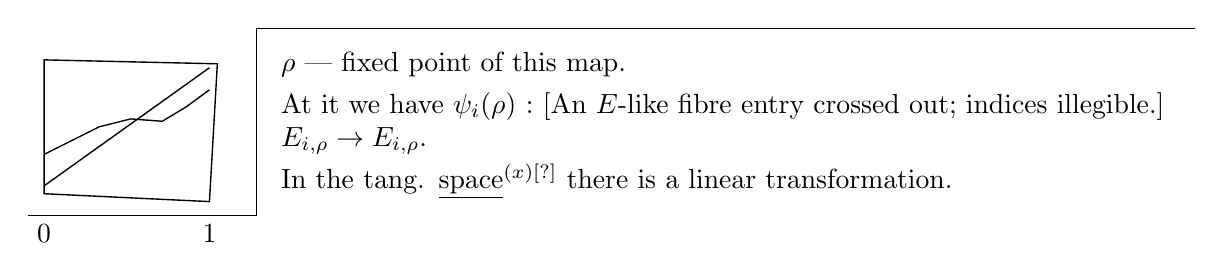
\begin{tikzpicture}[x=1mm,y=1mm,line width=.5pt]
\draw (5,4)--(27,3.5)--(26,-14)--(5,-13)--cycle;
\draw (5,-12)--(26,3);
\draw (5,-8)--(9,-6)--(12,-4.5)--(16,-3.5)--(20,-3.8)--(23,-2)--(26,.2);
\node at (5,-18) {$0$};
\node at (26,-18) {$1$};
\node[anchor=north west,align=left,inner sep=0pt,text width=114mm] (fixedtext) at (35,5) {
$\rho$ — fixed point of this map.\par\smallskip
At it we have $\psi_i(\rho):$
[An $E$-like fibre entry crossed out; indices illegible.]
$E_{i,\rho}\to E_{i,\rho}$.\par\smallskip
In the tang. \underline{space}\textsuperscript{$(x)$[?]} there is a linear transformation.
};
\draw ([xshift=2mm,yshift=3mm]fixedtext.north east)
 --([xshift=-3mm,yshift=3mm]fixedtext.north west)
 --([xshift=-3mm,yshift=-2mm]fixedtext.south west)--++(-29mm,0);
\end{tikzpicture}
\end{center}
\SourceFigure{GELFAND-P000094}{brouwer-graph}{Rectangle labelled $0$ and $1$, two ascending lines, dense crossing. The crossing geometry is unclear. An angular line runs above and to the left of the adjoining lines about $\rho$, the fibre and the tangent space, then extends left below the drawing.}
\SourceFigure{GELFAND-P000094}{fixed-point}{$\rho$ — fixed point of this map.}
\Unclear{GELFAND-P000094}{fixed-fibre-corrections}{Before the new $E_{i,\rho}$ an $E$-like entry with unread indices is cancelled. An insertion $(x)$[?] is above the underlined space; the precise letter is uncertain.}
\end{GelfandAdjacentEvidence}
\begin{GelfandAdjacentEvidence}{GELFAND-P000094}{11}

It is denoted $J_\rho(f)$ in the tang. space to $X$.
\SourceFigure{GELFAND-P000094}{tangent-J}{$J_\rho(f)$; in the tang. space to $X$.}
\end{GelfandAdjacentEvidence}
\begin{GelfandAdjacentEvidence}{GELFAND-P000094}{12}

The point is isolated $\Leftarrow$ it is sufficient that
\begin{equation*}\det(1-J_\rho(f))\ne0.\end{equation*}
(by the implicit-function theorem).
\SourceFigure{GELFAND-P000094}{isolation-criterion}{Heavy leftward arrow $\Leftarrow$; $\det(1-J_\rho(f))\ne0$; by the implicit-function theorem.}
\end{GelfandAdjacentEvidence}
\begin{GelfandAdjacentEvidence}{GELFAND-P000094}{13}

The point [short crossed-out word illegible] singular fixed, if it is $0$, regular, if $\ne0$.
\Unclear{GELFAND-P000094}{regular-point-cancel}{After point, a short word is densely cancelled; former letters cannot be recovered. Then singular fixed, if it is $0$, regular, if $\ne0$.}
\end{GelfandAdjacentEvidence}
\begin{GelfandAdjacentEvidence}{GELFAND-P000094}{14}

The graphs $(x,f(x))$ and $(x,x)$ intersect transversally.
\SourceFigure{GELFAND-P000094}{transverse-graphs}{$(x,f(x))$ and $(x,x)$; intersect transversally.}
\end{GelfandAdjacentEvidence}
\begin{GelfandAdjacentEvidence}{GELFAND-P000094}{15}

Consider the number
\begin{equation*}
\frac{\operatorname{tr}\psi_i(\rho)}{|\det(1-J_\rho(f))|}.
\end{equation*}
\SourceFigure{GELFAND-P000094}{local-trace}{$\operatorname{tr}\psi_i(\rho)$ above $|\det(1-J_\rho(f))|$.}
\end{GelfandAdjacentEvidence}
\begin{GelfandAdjacentEvidence}{GELFAND-P000094}{16}

At the point $\rho$ there are $2$ lin. transf. $\psi_i(\rho)$ — the fibre into itself,
and a transf. of the tang. space.
\SourceFigure{GELFAND-P000094}{two-maps}{At the point $\rho$ — $2$ lin. transf.; $\psi_i(\rho)$ — the fibre into itself; transf. of the tang. space.}
\end{GelfandAdjacentEvidence}
\begin{GelfandAdjacentEvidence}{GELFAND-P000094}{17}

\begin{equation*}
\sum(-1)^i\frac{\operatorname{tr}\psi_i(\rho)}{|\det(1-J_\rho(f))|}
=\sigma(\rho).
\end{equation*}
\SourceFigure{GELFAND-P000094}{local-contribution}{$\sum(-1)^i$ with no visible limits; $\operatorname{tr}\psi_i(\rho)$; $|\det(1-J_\rho(f))|$; $\sigma(\rho)$.}
\end{GelfandAdjacentEvidence}
\begin{GelfandAdjacentEvidence}{GELFAND-P000094}{18}

This number does not depend on the complex, but depends only on $f$ and the induced maps in the fibres
(but the map of fibres is not arbitrary, it must commute with the complex).
\SourceFigure{GELFAND-P000094}{complex-independence}{Does not depend on the complex; $f$ and induced maps in the fibres; in parentheses, but the map of fibres is not arbitrary, it must commute with the complex.}
\end{GelfandAdjacentEvidence}
\begin{GelfandAdjacentEvidence}{GELFAND-P000094}{19}

$\psi_i$ must be an endomorphism!
\SourceFigure{GELFAND-P000094}{endomorphism-warning}{$\psi_i$ must be an endomorphism!}
\end{GelfandAdjacentEvidence}




\begin{GelfandAdjacentEvidence}{GELFAND-P000095}{1}
\SourcePage{GELFAND-P000095}{64}
\underline{Theorem} of Atiyah–Bott.
\SourceFigure{GELFAND-P000095}{theorem-heading}{Only Theorem is underlined; Atiyah–Bott; number $64$.}
\end{GelfandAdjacentEvidence}
\begin{GelfandAdjacentEvidence}{GELFAND-P000095}{2}

Let there be an ellipt. complex $d$,
$f:X\to X$ and its lifting $\psi$, which is an endomorphism
of this complex. Then the formula holds
\SourceFigure{GELFAND-P000095}{theorem-assumptions}{Ellipt. complex $d$; $f:X\to X$; its lifting $\psi$, which is an endomorphism of this complex.}
\end{GelfandAdjacentEvidence}
\begin{GelfandAdjacentEvidence}{GELFAND-P000095}{3}

\begin{equation*}L(T,E)=\sum_\rho\sigma(\rho)\end{equation*}
over all fixed points.
\SourceFigure{GELFAND-P000095}{Lefschetz-local-formula}{$L(T,E)=\sum_\rho\sigma(\rho)$; over all fixed points.}
\end{GelfandAdjacentEvidence}
\begin{GelfandAdjacentEvidence}{GELFAND-P000095}{4}

$T$ is given by the pair $f$ and $\psi$.
\SourceFigure{GELFAND-P000095}{T-pair}{$T$ is given by the pair $f$ and $\psi$.}
\end{GelfandAdjacentEvidence}
\begin{GelfandAdjacentEvidence}{GELFAND-P000095}{5}

\underline{Proof.}
\SourceFigure{GELFAND-P000095}{proof-heading}{Proof is underlined.}
\end{GelfandAdjacentEvidence}
\begin{GelfandAdjacentEvidence}{GELFAND-P000095}{6}

First unclearly[?] and incompletely (ideas)
\Unclear{GELFAND-P000095}{proof-opening-word}{First word after First: unclearly[?] / inexactly[?]; crowded middle strokes.}
\end{GelfandAdjacentEvidence}
\begin{GelfandAdjacentEvidence}{GELFAND-P000095}{7}

$d:\Gamma(E)_i\longrightarrow\Gamma(E)_{i+1}$, construct a new operator from it.
\SourceFigure{GELFAND-P000095}{initial-d-map}{$d:\Gamma(E)_i\longrightarrow\Gamma(E)_{i+1}$; indices $i$, $i+1$ are outside the parentheses; construct a new operator from it.}
\end{GelfandAdjacentEvidence}
\begin{GelfandAdjacentEvidence}{GELFAND-P000095}{8}

Introduce a scalar product on $\Gamma(E)$.
\SourceFigure{GELFAND-P000095}{scalar-product}{Introduce a scalar product on $\Gamma(E)$.}
\end{GelfandAdjacentEvidence}
\begin{GelfandAdjacentEvidence}{GELFAND-P000095}{9}

Introduce the “Laplacian oper.”
\begin{equation*}\Box=d^*d+dd^*.\end{equation*}
\SourceFigure{GELFAND-P000095}{Laplacian}{Laplacian oper.; $\Box=d^*d+dd^*$.}
\end{GelfandAdjacentEvidence}
\begin{GelfandAdjacentEvidence}{GELFAND-P000095}{10}

Maps each $\Gamma(E)$ into itself.
\SourceFigure{GELFAND-P000095}{degree-preservation}{Maps each $\Gamma(E)$ into itself.}
\end{GelfandAdjacentEvidence}
\begin{GelfandAdjacentEvidence}{GELFAND-P000095}{11}

Hodge theorem (generalized): $\Box$ has a discr. positive
spectrum, to each eig. number corresponds a finite number of eig. values.
\SourceFigure{GELFAND-P000095}{Hodge-spectrum}{Discr. positive spectrum; to each eig. number corresponds a finite number of eig. values.}
\end{GelfandAdjacentEvidence}
\begin{GelfandAdjacentEvidence}{GELFAND-P000095}{12}

$\Gamma_\lambda(E_i)$ — subspace corresp. to the eig. value $\lambda$. (eig. functions)
\SourceFigure{GELFAND-P000095}{eigenspace-definition}{$\Gamma_\lambda(E_i)$; subspace corresp. to the eig. value $\lambda$; eig. functions.}
\end{GelfandAdjacentEvidence}
\begin{GelfandAdjacentEvidence}{GELFAND-P000095}{13}

\begin{equation*}d:\Gamma_\lambda(E_i)\longrightarrow\Gamma_\lambda(E_{i+1}).\end{equation*}
\SourceFigure{GELFAND-P000095}{restricted-d-map}{$d:\Gamma_\lambda(E_i)\longrightarrow\Gamma_\lambda(E_{i+1})$.}
\end{GelfandAdjacentEvidence}
\begin{GelfandAdjacentEvidence}{GELFAND-P000095}{14}

\begin{center}
\begin{tikzpicture}[x=1mm,y=1mm,line width=.45pt]
\node at (0,0) {$\Box d=d\Box$};
\node at (18,.5) {\scriptsize $i$[?]};
\draw (1,0) ellipse (23mm and 6mm);
\end{tikzpicture}
\end{center}
\Unclear{GELFAND-P000095}{commutation-oval}{$\Box d=d\Box$ in an oval; a separate small $i$-like stroke[?] is to the right of the last square.}
\end{GelfandAdjacentEvidence}
\begin{GelfandAdjacentEvidence}{GELFAND-P000095}{15}

\begin{equation*}
d:\Gamma(E_1)\longrightarrow\Gamma(E_2)\longrightarrow\cdots\longrightarrow\Gamma(E_n).
\end{equation*}
\SourceFigure{GELFAND-P000095}{full-complex}{$d:\Gamma(E_1)\to\Gamma(E_2)\to\cdots\to\Gamma(E_n)$.}
\end{GelfandAdjacentEvidence}
\begin{GelfandAdjacentEvidence}{GELFAND-P000095}{16}

Now consider
\begin{equation*}
d:\Gamma_\lambda(E_1)\longrightarrow\Gamma_\lambda(E_2)\longrightarrow\cdots\longrightarrow\Gamma_\lambda(E_n).
\end{equation*}
\SourceFigure{GELFAND-P000095}{eigen-complex}{Now consider; $d:\Gamma_\lambda(E_1)\to\Gamma_\lambda(E_2)\to\cdots\to\Gamma_\lambda(E_n)$.}
\end{GelfandAdjacentEvidence}
\begin{GelfandAdjacentEvidence}{GELFAND-P000095}{17}

$\Gamma_\lambda$ are already finite-dimensional ($d^2=0$), homologies
arise here too.
\SourceFigure{GELFAND-P000095}{finite-dimensional}{$\Gamma_\lambda$ are already finite-dimensional; $(d^2=0)$; homologies arise here too.}
\end{GelfandAdjacentEvidence}
\begin{GelfandAdjacentEvidence}{GELFAND-P000095}{18}

\begin{equation*}
H^i\{\Gamma_\lambda(E)\}=\begin{cases}H^i(E),&\lambda=0,\\0,&\lambda\ne0.\end{cases}
\end{equation*}
\SourceFigure{GELFAND-P000095}{eigen-cohomology}{$H^i\{\Gamma_\lambda(E)\}$; $H^i(E)$ at $\lambda=0$, $0$ at $\lambda\ne0$.}
\end{GelfandAdjacentEvidence}
\begin{GelfandAdjacentEvidence}{GELFAND-P000095}{19}

(indices exist only for defin.[?] oper.)
\Unclear{GELFAND-P000095}{index-operator-abbreviation}{Abbreviation after for: defin.[?] / diffin.[?]; unexpanded.}
\end{GelfandAdjacentEvidence}
\begin{GelfandAdjacentEvidence}{GELFAND-P000095}{20}

For the de Rham compl. — Hodge theorem — every [crossed-out expression illegible]
\SourceFigure{GELFAND-P000095}{de-rham-Hodge}{For the de Rham compl. — Hodge theorem — every.}
\end{GelfandAdjacentEvidence}
\begin{GelfandAdjacentEvidence}{GELFAND-P000095}{21}

[Crossed-out expression illegible] closed form
$\underset{\longrightarrow\,\longrightarrow}{\text{homologous}}$ to a harmonic one.
\Unclear{GELFAND-P000095}{harmonic-form-cancels}{Two densely crossed-out expressions: after every and before closed; former letters undetermined.}
\SourceFigure{GELFAND-P000095}{closed-form-statement}{Closed form homologous to a harmonic one; two short rightward arrows under homologous.}
\end{GelfandAdjacentEvidence}
\begin{GelfandAdjacentEvidence}{GELFAND-P000095}{22}

Calculate the trace: $\sum$ diag. elem. $\equiv\sum$ eig. values.
\SourceFigure{GELFAND-P000095}{trace-definition}{Calculate the trace; $\sum$ diag. elem. $\equiv\sum$ eig. values; three horizontal bars.}
\end{GelfandAdjacentEvidence}
\begin{GelfandAdjacentEvidence}{GELFAND-P000095}{23}

(1. Trace as $\int K(x,x)\,dx$, and $\sum$ of traces in each subspace
\SourceFigure{GELFAND-P000095}{kernel-trace}{$(1.$; trace as $\int K(x,x)\,dx$; and $\sum$ of traces in each subspace.}
\end{GelfandAdjacentEvidence}
\begin{GelfandAdjacentEvidence}{GELFAND-P000095}{24}

(inv. eig.)
\SourceFigure{GELFAND-P000095}{invariant-parenthesis}{Inv. eig. in parentheses.}
\end{GelfandAdjacentEvidence}
\begin{GelfandAdjacentEvidence}{GELFAND-P000095}{25}

$\lambda\ne0$ [short sign densely crossed out, illegible] no trace, $\lambda=0$ calc. through homologies. $\Bigg\}$[?]
\Unclear{GELFAND-P000095}{nonzero-trace-cancel}{After $\lambda\ne0$, a short sign / arrow[?] is densely cancelled. No trace is legible, then $\lambda=0$ calc. through homologies. A large closing bracket-like sign at right: brace / parenthesis[?].}
\end{GelfandAdjacentEvidence}




\begin{GelfandAdjacentEvidence}{GELFAND-P000096}{1}
\SourcePage{GELFAND-P000096}{unlabelled}
$11/\overline{\underline{\mathrm X}}$ \uwave{Seminar} \uwave{plan.}
\SourceFigure{GELFAND-P000096}{date-heading}{$11/\overline{\underline{\mathrm X}}$; upper and lower bars at $X$; Seminar and plan have wavy underlining.}
\end{GelfandAdjacentEvidence}
\begin{GelfandAdjacentEvidence}{GELFAND-P000096}{2}

1. Integro-diff. operators (Agranovich).
(2 hours)
\SourceFigure{GELFAND-P000096}{plan-operators}{Integro-diff. operators; Agranovich; beneath the parenthesis, (2 hours).}
\end{GelfandAdjacentEvidence}
\begin{GelfandAdjacentEvidence}{GELFAND-P000096}{3}

2. Atiyah–Singer on the index.
Kirillov or Gelfand. Dynin.
(yearly sem. Cartan-Schwartz
and Vishik’s sem. 64–65.)
\SourceFigure{GELFAND-P000096}{plan-index}{Atiyah–Singer on the index; Kirillov or Gelfand; Dynin; yearly sem. Cartan-Schwartz and Vishik’s sem. $64$–$65$.}
\end{GelfandAdjacentEvidence}
\begin{GelfandAdjacentEvidence}{GELFAND-P000096}{4}

3. Statistical physics ($\underset{\text{Robert Adl’fovich[?]}}{\text{Minlos}}$, 3 meetings).
\SourceFigure{GELFAND-P000096}{plan-physics}{Statistical physics; Minlos; $3$ meetings; first name and patronymic below the surname.}
\Unclear{GELFAND-P000096}{minlos-patronymic}{Below Minlos: Robert Adl’fovich[?] / Robert Adol’fovich[?]; the small loop after d is uncertain.}
\end{GelfandAdjacentEvidence}
\begin{GelfandAdjacentEvidence}{GELFAND-P000096}{5}

4. Adeles and adele groups (Graev [crossed-out M-like sign, illegible] Mark Iosifovich).
(2 meetings)
\SourceFigure{GELFAND-P000096}{plan-adeles}{Adeles and adele groups; Graev Mark Iosifovich; $(2$ meetings$)$.}
\Unclear{GELFAND-P000096}{graev-initial-cancel}{Between Graev and Mark, an M-like sign is densely cancelled; former reading undetermined.}
\end{GelfandAdjacentEvidence}
\begin{GelfandAdjacentEvidence}{GELFAND-P000096}{6}

5. Linear algebraic groups.
Kirillov
Gelfand
\SourceFigure{GELFAND-P000096}{plan-groups}{Linear algebraic groups; Kirillov / Gelfand in a column at right.}
\end{GelfandAdjacentEvidence}
\begin{GelfandAdjacentEvidence}{GELFAND-P000096}{7}

6. Work of Bott and Chern (Acta Math.) Gelfand
Vol. 114[?] $N=1$–$2$
\SourceFigure{GELFAND-P000096}{plan-bott-chern}{Work of Bott and Chern; Acta Math.; Gelfand; volume notation below the journal name.}
\Unclear{GELFAND-P000096}{chern-volume-correction}{Dense volume signs: Vol. 114[?] / Vol. III[?]; $N=1$–$2$. A short sign / word is crossed out below.}
\end{GelfandAdjacentEvidence}
\begin{GelfandAdjacentEvidence}{GELFAND-P000096}{8}

(transfer[?] of Nevanlinna’s theorem on zeros of funct. to [densely crossed-out fragment illegible] curves
sect. of vect. sheaves.)
\Unclear{GELFAND-P000096}{nevanlinna-cancel}{First word in parentheses transfer[?] / transferred[?]. A fragment is densely cancelled before curves; then sect. of vect. sheaves.}
\end{GelfandAdjacentEvidence}
\begin{GelfandAdjacentEvidence}{GELFAND-P000096}{9}

7. Riem\underline{ann–Roch}–\underline{Grothen}dieck theorem. Kazdan[?] D. A.
\Unclear{GELFAND-P000096}{plan-riemann-roch}{Two straight underlines below parts of the title: the ann–Roch area and the start of Grothendieck; precise boundaries uncertain. Surname Kazdan[?] / Kazhdan[?].}
\end{GelfandAdjacentEvidence}
\begin{GelfandAdjacentEvidence}{GELFAND-P000096}{10}

\uwave{Kazdan[?].} Riemann–Roch theorem.
\Unclear{GELFAND-P000096}{kazhdan-heading}{The surname with a wavy underline: Kazdan[?] / Kazhdan[?]; dense sign between a and d.}
\end{GelfandAdjacentEvidence}
\begin{GelfandAdjacentEvidence}{GELFAND-P000096}{11}

To a vect. sheaf corresp. a cohom. class — Chern class.
\SourceFigure{GELFAND-P000096}{Chern-class}{To a vect. sheaf corresp. a cohom. class; Chern class, the Latin surname with a Russian ending in the source.}
\end{GelfandAdjacentEvidence}
\begin{GelfandAdjacentEvidence}{GELFAND-P000096}{12}

\underline{Chern classes.}
\SourceFigure{GELFAND-P000096}{Chern-heading}{Chern classes is underlined; the start of classes is written densely.}
\end{GelfandAdjacentEvidence}
\begin{GelfandAdjacentEvidence}{GELFAND-P000096}{13}

$X$ — classical alg. variety, aff. space
\SourceFigure{GELFAND-P000096}{affine-space}{$X$ — classical alg. variety, aff. space.}
\end{GelfandAdjacentEvidence}
\begin{GelfandAdjacentEvidence}{GELFAND-P000096}{14}

alg. funct. on it — polynomials, this is the simplest[?]
alg. variety.
\Unclear{GELFAND-P000096}{polynomial-functions}{Alg. funct. on it — polynomials; this is the simplest[?] / this is the most simple[?]; ending of the last word dense; then alg. variety.}
\end{GelfandAdjacentEvidence}
\begin{GelfandAdjacentEvidence}{GELFAND-P000096}{15}

Affine alg. varieties. Let a collection
of polynomials be given
\begin{equation*}p_1(x_1,\ldots,x_n),\ldots,p_k(x_1,\ldots,x_n)\end{equation*}
\SourceFigure{GELFAND-P000096}{affine-polynomials}{Affine alg. varieties; collection of polynomials $p_1(x_1,\ldots,x_n),\ldots,p_k(x_1,\ldots,x_n)$.}
\end{GelfandAdjacentEvidence}
\begin{GelfandAdjacentEvidence}{GELFAND-P000096}{16}

(let the field $K$ be alg. closed)
\SourceFigure{GELFAND-P000096}{ground-field}{Let the field $K$ be alg. closed; uppercase $K$.}
\end{GelfandAdjacentEvidence}
\begin{GelfandAdjacentEvidence}{GELFAND-P000096}{17}

Consider collections of points — satisfy an eqn., aff. alg. var.-
\SourceFigure{GELFAND-P000096}{solution-sets}{Consider collections of points; satisfy an eqn.; aff. alg. var.- with a final dash.}
\end{GelfandAdjacentEvidence}
\begin{GelfandAdjacentEvidence}{GELFAND-P000096}{18}

— alg. funct. — restrictions of polynomials —
\SourceFigure{GELFAND-P000096}{restrictions}{— Alg. funct. — restrictions of polynomials —.}
\end{GelfandAdjacentEvidence}
\begin{GelfandAdjacentEvidence}{GELFAND-P000096}{19}

— quotient ring by the ideal spanned by polyn.
\SourceFigure{GELFAND-P000096}{quotient-ring}{Quotient ring by the ideal spanned by polyn.}
\end{GelfandAdjacentEvidence}
\begin{GelfandAdjacentEvidence}{GELFAND-P000096}{20}

Alg. prevariety — space loc. isomorphic
to an aff. variety.
\SourceFigure{GELFAND-P000096}{prevariety}{Alg. prevariety; space loc. isomorphic to an aff. variety.}
\end{GelfandAdjacentEvidence}




\begin{GelfandAdjacentEvidence}{GELFAND-P000097}{1}
\SourcePage{GELFAND-P000097}{65}
If add. conditions
\begin{equation*}\begin{gathered}Q_1(x_1,\ldots,\underline{x_n)}\ne0,\\Q_i(x_1,\ldots,x_n)\ne0,\end{gathered}\end{equation*}
\Unclear{GELFAND-P000097}{nonzero-conditions}{$Q_1$, $Q_i$; $x_n)$ underlined in the first line. Between the lines below $Q_1$, a dot $\cdot$, and a short dash $-$ farther right; their role is undetermined. At right, (all at once $\ne0$).}
\Unclear{GELFAND-P000097}{nonzero-top-cancel}{Two lines at right are densely crossed out; an initial parenthesis, loops, horizontal and slanting strokes remain visible; no reliable reading established.}
\end{GelfandAdjacentEvidence}
\begin{GelfandAdjacentEvidence}{GELFAND-P000097}{2}

(all at once $\ne0$)
then also an alg. var.
\SourceFigure{GELFAND-P000097}{algebraic-set}{Then also an alg. var.}
\end{GelfandAdjacentEvidence}
\begin{GelfandAdjacentEvidence}{GELFAND-P000097}{3}

funct. — from rat. funct. with poles outside these points.
\SourceFigure{GELFAND-P000097}{rational-functions}{Funct. — from rat. funct. with poles outside these points.}
\end{GelfandAdjacentEvidence}
\begin{GelfandAdjacentEvidence}{GELFAND-P000097}{4}

\underline{Example:} line, alg. funct. — polynomials.
\SourceFigure{GELFAND-P000097}{example-line}{Example is underlined; line, alg. funct. — polynomials.}
\end{GelfandAdjacentEvidence}
\begin{GelfandAdjacentEvidence}{GELFAND-P000097}{5}

Space given with a stock of funct.
\SourceFigure{GELFAND-P000097}{space-functions}{Space given with a stock of funct.}
\end{GelfandAdjacentEvidence}
\begin{GelfandAdjacentEvidence}{GELFAND-P000097}{6}

Consider points $x\ne0$. Funct. now $\frac{P(x)}{x^m}$[?].
\Unclear{GELFAND-P000097}{punctured-line}{Consider points $x\ne0$; fraction $\frac{P(x)}{x^m}$[?]. The denominator exponent is $m$- / $n$-like and written densely.}
\end{GelfandAdjacentEvidence}
\begin{GelfandAdjacentEvidence}{GELFAND-P000097}{7}

Aff. var. — zeros of some funct. and others do not turn into $0$.
\SourceFigure{GELFAND-P000097}{affine-nonzero}{Aff. var. — zeros of some funct. and others do not turn into $0$.}
\end{GelfandAdjacentEvidence}
\begin{GelfandAdjacentEvidence}{GELFAND-P000097}{8}

\underline{General alg. var.}: $\forall$ point there exists an open nbhd.,
isomorphic to an aff. alg. variety.
(at first only a diff. var. or ringed space)
\SourceFigure{GELFAND-P000097}{general-variety}{General alg. var. underlined; $\forall$ point, open nbhd., isomorphic to an aff. alg. variety; below, parentheses concerning a diff. var. or ringed space.}
\end{GelfandAdjacentEvidence}
\begin{GelfandAdjacentEvidence}{GELFAND-P000097}{9}

Ringed space — [short crossed-out fragment illegible]
\Unclear{GELFAND-P000097}{ringed-space-cancel}{Between the dash and var., a short sign / word is densely cancelled; reading undetermined.}
\end{GelfandAdjacentEvidence}
\begin{GelfandAdjacentEvidence}{GELFAND-P000097}{10}

$\underset{\text{(space)}}{\text{var.}}$ with a sheaf of rings.
\SourceFigure{GELFAND-P000097}{ringed-space-definition}{Var. with a sheaf of rings; (space) inserted below var.}
\end{GelfandAdjacentEvidence}
\begin{GelfandAdjacentEvidence}{GELFAND-P000097}{11}

Every aff. alg. var. — ringed space.
\SourceFigure{GELFAND-P000097}{ringed-affine}{Every aff. alg. var. — ringed space.}
\end{GelfandAdjacentEvidence}
\begin{GelfandAdjacentEvidence}{GELFAND-P000097}{12}

On it one introduces the Zariski top. (So that all alg. funct.
are cont. — closed sets — zeros of a finite
number of alg. funct. $/$[?].
\Unclear{GELFAND-P000097}{zariski-topology}{Zariski top.; opening parenthesis before So that; after alg. funct., a slash $/$[?] / closing parenthesis $)$[?], then a period.}
\end{GelfandAdjacentEvidence}
\begin{GelfandAdjacentEvidence}{GELFAND-P000097}{13}

Sheaf of rings — an open set
in it this is also an alg. variety.
\SourceFigure{GELFAND-P000097}{open-sheaf}{Sheaf of rings — an open set in it this is also an alg. variety.}
\Unclear{GELFAND-P000097}{left-margin-traces}{In the left margin, faint, dotted and loop-like traces; before the following formula, a dense A-like sign. No reliable complete words read; origin of the traces undetermined.}
\end{GelfandAdjacentEvidence}
\begin{GelfandAdjacentEvidence}{GELFAND-P000097}{14}

$C^2\setminus0$ is not an aff. alg. variety.
\SourceFigure{GELFAND-P000097}{punctured-plane}{$C^2\setminus0$ is not an aff. alg. variety; written $C$, without an additional vertical bar.}
\end{GelfandAdjacentEvidence}
\begin{GelfandAdjacentEvidence}{GELFAND-P000097}{15}

Every $\overset{\underbrace{\text{open set}}}{\text{aff.}}$ alg. variety[?] cont… [ending crossed out]
\SourceFigure{GELFAND-P000097}{open-insertion}{Above aff., open set is inserted with a lower brace and a downward point; insertion position retained.}
\Unclear{GELFAND-P000097}{open-variety-word}{Ending of the word variety: handwritten -iya[?] / -iye[?]; last sign ya-/e-like.}
\Unclear{GELFAND-P000097}{open-variety-cancel}{Cont…: the ending is densely crossed out; zhit-like letter tops remain above the strokes[?]. Possible whole word contains[?]; cancelled letters not securely determined.}
\end{GelfandAdjacentEvidence}
\begin{GelfandAdjacentEvidence}{GELFAND-P000097}{16}

open subset, being an alg. variety.
\SourceFigure{GELFAND-P000097}{open-subvariety}{Open subset, being an alg. variety.}
\end{GelfandAdjacentEvidence}
\begin{GelfandAdjacentEvidence}{GELFAND-P000097}{17}

\uwave{Sheaf} [n-/i-like sign, illegible] of rings — must def. the group of sections
\Unclear{GELFAND-P000097}{sheaf-prefix-mark}{Sheaf has a wavy underline. Before of rings, a separate dense n-/i-like sign; whether cancellation or insertion is undetermined.}
\end{GelfandAdjacentEvidence}
\begin{GelfandAdjacentEvidence}{GELFAND-P000097}{18}

on basic open sets obtained by eqns. of the form
$R_2(x)\ne0$[?], the ring of alg. funct. on this set.
\Unclear{GELFAND-P000097}{sheaf-basis}{The group of sections on basic open sets; eqns. of the form $R_2(x)\ne0$[?] / $R_1(x)\ne0$[?]; subscript with a curved top and a long base, $2$-like. Then the ring of alg. funct. on this set.}
\end{GelfandAdjacentEvidence}
\begin{GelfandAdjacentEvidence}{GELFAND-P000097}{19}

Obtain a sheaf of germs of alg. funct. ringed space.
\SourceFigure{GELFAND-P000097}{germs}{Obtain a sheaf of germs of alg. funct. ringed space; no separate comma visible after funct.}
\end{GelfandAdjacentEvidence}
\begin{GelfandAdjacentEvidence}{GELFAND-P000097}{20}

Ringed space — prealg.[?] var., if it
is loc. isomorphic to an aff. alg. var.
(as a ringed space)
\Unclear{GELFAND-P000097}{prevariety-definition}{Abbreviation after the dash prealg.[?] / prev.[?]; dense letters after pred. In the next line loc. is written densely; then isomorphic to an aff. alg. var.; below, (as a ringed space).}
\end{GelfandAdjacentEvidence}




\begin{GelfandAdjacentEvidence}{GELFAND-P000098}{1}
\SourcePage{GELFAND-P000098}{unlabelled}

Aff. alg. var.

\begin{equation*}\begin{gathered}\left\{\begin{array}{l}p_1={}\\\vdots\\p_m=0\end{array}\right.\\Q\ne0\end{gathered}\end{equation*}

[Crossed out: open[?], remainder illegible] closed set.

\Unclear{GELFAND-P000098}{affine-opening-cancel}{Under the left brace, $p_1=$ with no visible right-hand side, dots, $p_m=0$; below, $Q\ne0$. At right, dense cancellation before closed set; otkr.-like remnants (open)[?], full reading undetermined.}
\end{GelfandAdjacentEvidence}
\begin{GelfandAdjacentEvidence}{GELFAND-P000098}{2}


$R_i(x_1,\ldots,x_n)=0$. $R_i$ — polynomials.

\SourceFigure{GELFAND-P000098}{closed-polynomials}{Closed set; $R_i(x_1,\ldots,x_n)=0$, $R_i$ — polynomials.}
\end{GelfandAdjacentEvidence}
\begin{GelfandAdjacentEvidence}{GELFAND-P000098}{3}


Basis of open sets — one condition $U_S:S\ne0$.
(such is cont. in every open —
— leave $1$ condition).

\SourceFigure{GELFAND-P000098}{basic-open}{$U_S:S\ne0$; in parentheses two separate dashes: after open and before leave $1$ condition.}
\end{GelfandAdjacentEvidence}
\begin{GelfandAdjacentEvidence}{GELFAND-P000098}{4}


The group of sections is given thus —

\SourceFigure{GELFAND-P000098}{sections-definition}{The group of sections is given thus —; then $\Gamma(U_S)$ and rat. funct. on $R^n$. Written $R$, without an additional vertical bar.}
\end{GelfandAdjacentEvidence}
\begin{GelfandAdjacentEvidence}{GELFAND-P000098}{5}


$\Gamma(U_S)$ — all rat. funct. on $R^n$ which do not turn into $\infty$
anywhere on our set.

\begin{equation*}\Gamma(U_S)\mathrel{=\!\text{[?]}}\left\{\frac{P(x)}{Q(x)}\right\}\end{equation*}

\Unclear{GELFAND-P000098}{sections-relation-overwrite}{Between $\Gamma(U_S)$ and the brace, two horizontal bars with dense overwriting between them: $=$ with alteration / rewritten sign; $\ne$ remains an unestablished alternative. No definite diagonal stroke read.}

\SourceFigure{GELFAND-P000098}{rational-quotient}{$\Gamma(U_S)$, overwritten sign, $\left\{\frac{P(x)}{Q(x)}\right\}$; no separate period visible after the right brace.}
\end{GelfandAdjacentEvidence}
\begin{GelfandAdjacentEvidence}{GELFAND-P000098}{6}


Identify, if on $U_S$ one value.
This is a ring.

\SourceFigure{GELFAND-P000098}{sections-identification}{Identify, if on $U_S$ one value.}
\end{GelfandAdjacentEvidence}
\begin{GelfandAdjacentEvidence}{GELFAND-P000098}{7}


(This will be a sheaf, easy to prove that this will real\underline{ly}
be the gr. of sections.)

\Unclear{GELFAND-P000098}{ring-sheaf}{This is a ring. In parentheses: This will be a sheaf, easy to prove that this will really be the gr. of sections. A short horizontal stroke lies below the final letter of the translated really; its role is undetermined. The upper breve belongs to the source letter y-short.}
\end{GelfandAdjacentEvidence}
\begin{GelfandAdjacentEvidence}{GELFAND-P000098}{8}


Isom. of sheaves. obtained by the definition of an isomorphism

\SourceFigure{GELFAND-P000098}{isomorphism-intro}{Isom. of sheaves. obtained by the definition of an isomorphism; period after sheaves.}
\end{GelfandAdjacentEvidence}
\begin{GelfandAdjacentEvidence}{GELFAND-P000098}{9}


of bases[?]
homeom. nat.

\Unclear{GELFAND-P000098}{isomorphism-base-word}{At the line end, baz.[?] / bez.[?]; the middle letter has a loop, the last a descending stroke. Next line: homeom. nat.; the abbreviation remains uncertain.}
\end{GelfandAdjacentEvidence}
\begin{GelfandAdjacentEvidence}{GELFAND-P000098}{10}


\begin{center}
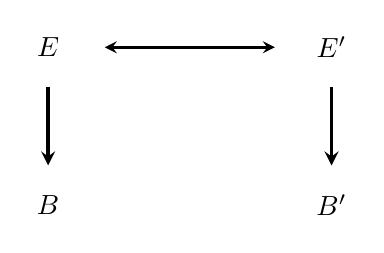
\begin{tikzpicture}[x=12mm,y=10mm,>=stealth]
\node (EL) at (0,0) {$E$};\node (ER) at (3,0) {$E'$};
\node (BL) at (0,-2) {$B$};\node (BR) at (3,-2) {$B'$};
\draw[<->,line width=0.9pt] (0.6,0) -- (2.4,0);
\draw[->,line width=1.2pt] (0,-0.5) -- (0,-1.5);
\draw[->,line width=1.2pt] (3,-0.5) -- (3,-1.5);
\end{tikzpicture}
\end{center}

\Unclear{GELFAND-P000098}{sheaf-isomorphism-diagram}{Top row $E\leftrightarrow E^{\prime}$, two heavy downward arrows to $B$, $B^{\prime}$. The upper ends and arrowheads are dense; their exact outlines are undetermined. No horizontal arrow visible between $B$ and $B^{\prime}$.}
\end{GelfandAdjacentEvidence}
\begin{GelfandAdjacentEvidence}{GELFAND-P000098}{11}


If $E$ is a subsheaf of funct., then
$B\longrightarrow B^{\prime}$ induces $E^{\prime}\longrightarrow E$.

\SourceFigure{GELFAND-P000098}{contravariance}{In the line, $B\longrightarrow B^{\prime}$ induces $E^{\prime}\longrightarrow E$; the prime strokes are raised at the second letters.}
\end{GelfandAdjacentEvidence}
\begin{GelfandAdjacentEvidence}{GELFAND-P000098}{12}


(A priori only commut.) Require that the isom.
be an isom. arising from considerations of the base. (natural!)
simply coincidence!

\SourceFigure{GELFAND-P000098}{base-isomorphism}{(A priori only commut.) Require that the isom. be an isom. arising from considerations of the base. (natural!) simply coincidence!}
\end{GelfandAdjacentEvidence}
\begin{GelfandAdjacentEvidence}{GELFAND-P000098}{13}


$C^2\setminus0$ is a
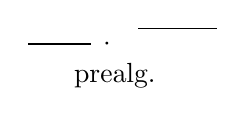
\begin{tikzpicture}[baseline=(w.base),x=1mm,y=1mm]
\node[inner sep=0pt] (w) at (0,0) {prealg.};
\draw[line width=0.4pt] (-11,4) -- (-3,4);
\draw[line width=0.4pt] (3,6) -- (13,6);
\node[inner sep=0pt] at (-1,4) {$\cdot$};
\end{tikzpicture}
var.

\Unclear{GELFAND-P000098}{punctured-prevariety}{$C^2\setminus0$ is a prealg. var. Above prealg., two separated horizontal strokes, the right higher; a dot beside the lower. Their role and association with the words are undetermined. Written $C$, without an additional vertical bar.}
\end{GelfandAdjacentEvidence}
\begin{GelfandAdjacentEvidence}{GELFAND-P000098}{14}


Choose $2$ straight lines[?].

\Unclear{GELFAND-P000098}{two-lines-word}{After Choose 2, cramped pryamye (straight lines)[?] / pryamki[?]; the middle and final strokes are dense.}
\end{GelfandAdjacentEvidence}
\begin{GelfandAdjacentEvidence}{GELFAND-P000098}{15}


$1$st on $x\ne0$, $2$nd $y\ne0$.
Our set — their union. Each of
them an aff. var.

\SourceFigure{GELFAND-P000098}{two-open-cover}{$1$st on $x\ne0$, $2$nd $y\ne0$. Our set — their union; each of them an aff. var.}
\end{GelfandAdjacentEvidence}
\begin{GelfandAdjacentEvidence}{GELFAND-P000098}{16}


\begin{center}
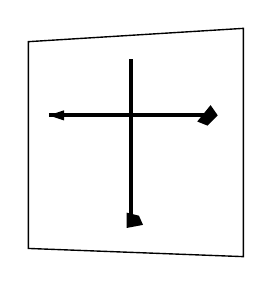
\begin{tikzpicture}[x=13mm,y=13mm]
\draw[line width=0.5pt] (0,0) -- (2.1,-0.08) -- (2.1,2.15) -- (0,2.02) -- cycle;
\draw[line width=1.5pt] (1,0.25) -- (1,1.85);
\draw[line width=1.5pt] (0.2,1.3) -- (1.8,1.3);
\path[fill=black] (0.2,1.3) -- (0.35,1.35) -- (0.35,1.25) -- cycle;
\path[fill=black] (1.65,1.24) -- (1.78,1.4) -- (1.85,1.3) -- (1.75,1.2) -- cycle;
\path[fill=black] (0.96,0.35) -- (1.08,0.32) -- (1.12,0.23) -- (0.96,0.2) -- cycle;
\end{tikzpicture}
\end{center}

\Unclear{GELFAND-P000098}{punctured-plane-diagram}{Within a rectangular frame, heavy vertical and horizontal lines intersect. The left end is pointed, the right and lower ends thickened; the role of the thickenings and exact form of possible arrowheads are undetermined. No letter labels or separate circle visible at the intersection.}
\end{GelfandAdjacentEvidence}
\begin{GelfandAdjacentEvidence}{GELFAND-P000098}{17}


Then agr\underline{ee.} sh\underline{eaves} of rings already clear[?].

\Unclear{GELFAND-P000098}{sheaf-agreement}{Then agree. sheaves of rings already clear[?]; final word clear[?] / easy[?]. Below the line are two separate strokes, under the end of agree. and part of sheaves; exact association of the underlining remains uncertain.}
\end{GelfandAdjacentEvidence}
\begin{GelfandAdjacentEvidence}{GELFAND-P000098}{18}


Points of $\overset{\text{pre}}{\vee}$ alg. var. may be inseparable for funct.

\SourceFigure{GELFAND-P000098}{inseparable-points}{Above the gap before alg., pre is inserted with a V-shaped insertion mark. Points is written densely; next-line ending funct.}
\end{GelfandAdjacentEvidence}
\begin{GelfandAdjacentEvidence}{GELFAND-P000098}{19}


\uwave{Example of pr. aff. $\overset{\underbrace{\text{pre-}}}{\text{alg.}}$ var.}

\SourceFigure{GELFAND-P000098}{example-heading}{The heading Example of pr. aff. alg. var. has a wavy underline. Above alg., pre- is inserted with a lower curly brace. The abbreviation pr. is not expanded.}
\end{GelfandAdjacentEvidence}
\begin{GelfandAdjacentEvidence}{GELFAND-P000098}{20}


\begin{equation*}\begin{gathered}
p_1(x_1,\ldots,x_n\text{[?]})=0,\\[-2pt]
\mathord{,}\quad-\qquad-\ \text{[?]}\\[-2pt]
p_k(x_1,\ldots,x_n\text{[?]})=0,\\
Q(x_1,\ldots,x_n\text{[?]})\ne0.
\end{gathered}\end{equation*}

\Unclear{GELFAND-P000098}{last-coordinate-indices}{In the three lines, the final indices $x_n$[?] / $x_m$[?] are dense; in the second line there is an additional upper stroke. The subscript $1$ on the first $p$ has a dense horizontal base. Between the first and second lines, three separate short marks: the left comma-/dot-like, and two dashes; their role is undetermined.}
\end{GelfandAdjacentEvidence}
\begin{GelfandAdjacentEvidence}{GELFAND-P000098}{21}


The last cond. is not obligatory, any [crossed-out word illegible]
aff. alg. var. can be given without using these
[crossed-out word illegible] conditions
($\exists$ var., isomorphic to it).

\Unclear{GELFAND-P000098}{affine-condition-cancels}{After any, a word densely cancelled with long horizontal strokes and a loop at left; below, after these, a second densely crossed-out word. No secure letter-by-letter reading of either established.}

\SourceFigure{GELFAND-P000098}{final-affine-condition}{The last cond. is not obligatory; then without using these … conditions; below, ($\exists$ var., isomorphic to it). The source ending usloviyakh is retained.}
\end{GelfandAdjacentEvidence}





\begin{GelfandAdjacentEvidence}{GELFAND-P000099}{1}
\SourcePage{GELFAND-P000099}{66}

Take $(x,y)$ with the condition

\begin{equation*}\begin{cases}P_i(x)=0,\\Q(x)y-1=0\end{cases}\end{equation*}

\hfill $(x_1,\ldots,x_n,y)$

\SourceFigure{GELFAND-P000099}{opening-graph}{System with a left brace: $P_i(x)=0$, $Q(x)y-1=0$. At the upper right, $(x_1,\ldots,x_n,y)$; the number $66$ with an angular stroke to its left and below.}
\end{GelfandAdjacentEvidence}
\begin{GelfandAdjacentEvidence}{GELFAND-P000099}{2}


They are isomorphic.

\SourceFigure{GELFAND-P000099}{isomorphic}{They are isomorphic.}
\end{GelfandAdjacentEvidence}
\begin{GelfandAdjacentEvidence}{GELFAND-P000099}{3}


Let there be a rng.[?] $P(x)$ and an ideal $I\text{[?]}$ — the first aff. alg. var.
$P(y)$ $J$ — the $2$nd aff. alg. var.

Their product —
— the ring $P(x,y)$ with the ideal

\begin{equation*}\left\{I\text{[?]}\otimes[P(y)]\mathbin{+\!\text{[?]}}[P(x)]\otimes J\right\}\end{equation*}

\Unclear{GELFAND-P000099}{product-ideal-notation}{The first ideal $I$[?] / $J$[?]: upper bar and lower left hook, with a lower loop in the formula. Between the summands, a densely overwritten $+$[?] / $\oplus$[?]. The abbreviation before the first ring is kol.[?] / kol\textquotesingle.[?].}

\SourceFigure{GELFAND-P000099}{product-intro}{Their product — and the following line — the ring $P(x,y)$ with the ideal: two separate dashes.}
\end{GelfandAdjacentEvidence}
\begin{GelfandAdjacentEvidence}{GELFAND-P000099}{4}


\hfill{\fontencoding{OT1}\fontfamily{cmr}\selectfont\textcircled{?}}\,[?]

\Unclear{GELFAND-P000099}{tensor-circled-symbol}{At right, a circled ?-/2-like sign; a separate lower dot below the main curved stroke. Reading undetermined.}
\end{GelfandAdjacentEvidence}
\begin{GelfandAdjacentEvidence}{GELFAND-P000099}{5}


(as a set — the usual prod.)

\SourceFigure{GELFAND-P000099}{product-set}{(as a set — the usual prod.).}
\end{GelfandAdjacentEvidence}
\begin{GelfandAdjacentEvidence}{GELFAND-P000099}{6}


The ring of funct. on it — the tensor pr. of the rings of funct. on those var.

\SourceFigure{GELFAND-P000099}{function-ring}{The ring of funct. on it — the tensor pr. of the rings of funct. on those var.}
\end{GelfandAdjacentEvidence}
\begin{GelfandAdjacentEvidence}{GELFAND-P000099}{7}


Pr. prod. of any prealg. var. — [crossed-out text illegible]

\begin{center}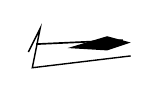
\begin{tikzpicture}[x=1mm,y=1mm]
\draw[line width=0.5pt] (0,2) -- (1.5,5) -- (0.5,0) -- (13,1.5);
\draw[line width=0.6pt] (1,3) -- (12,3.5);
\path[fill=black] (5,2.5) -- (10,4) -- (13,3.2) -- (10,2.2) -- cycle;
\end{tikzpicture}\end{center}

\SourceFigure{GELFAND-P000099}{product-heading}{Pr. prod. of any prealg. var. —. The abbreviation Pr. is retained.}
\end{GelfandAdjacentEvidence}
\begin{GelfandAdjacentEvidence}{GELFAND-P000099}{8}


$X,Y$ — $\overset{\text{pre}}{\vee}$alg. varieties.

\SourceFigure{GELFAND-P000099}{prevariety-insertion}{Above the gap before alg., pre is inserted, with a V-shaped insertion mark below; in the line, $X,Y$.}
\end{GelfandAdjacentEvidence}
\begin{GelfandAdjacentEvidence}{GELFAND-P000099}{9}


$\{U_i\}$ $\{V_j\}$ — $2$ covers by aff. open subvarieties.
$X\times Y$ is covered by $U_i\times V_j$. This is a napr.[?] var.

\Unclear{GELFAND-P000099}{affine-covers}{Upper line: $\{U_i\}$, $\{V_j\}$ — $2$ covers by aff. open subvarieties; below, $X\times Y$ is covered by $U_i\times V_j$. After This is, a napr.[?]-like abbreviation, read uncertainly.}
\end{GelfandAdjacentEvidence}
\begin{GelfandAdjacentEvidence}{GELFAND-P000099}{10}


[Densely crossed-out initial text illegible] Note that the prod. of var. is not the prod. of
top. spaces (the top. is not the top. of the prod.).

\Unclear{GELFAND-P000099}{product-and-heading-cancels}{After the dash in the product line, dense cancellation; below, a separate angular stroke and a black mark. Before Note, initial text is densely crossed out. Letter-by-letter readings of the cancellations undetermined.}

\SourceFigure{GELFAND-P000099}{product-topology}{Note that the prod. of var. is not the prod. of top. spaces (the top. is not the top. of the prod.).}
\end{GelfandAdjacentEvidence}
\begin{GelfandAdjacentEvidence}{GELFAND-P000099}{11}



Consider $X\times X$. Choose in it\par
\hspace*{12mm}{\small in it a struct.}

\SourceFigure{GELFAND-P000099}{structure-line}{In the line: Consider $X\times X$. Choose in it; below the line, separately, in it a struct.}
\end{GelfandAdjacentEvidence}
\begin{GelfandAdjacentEvidence}{GELFAND-P000099}{12}


Prealg.[?] subvar. — a closed subset in the top.[?] of Zariski.
It is itself a prealg. var.

\Unclear{GELFAND-P000099}{subvariety-prefix-correction}{At the beginning, Prealg.[?]; the middle letters are densely overwritten; earlier strokes unread.}

\Unclear{GELFAND-P000099}{subvariety-definition}{Subvar. — a closed subset in the top.[?] of Zariski. The source abbreviation tp.[?] / top.[?] is cramped. Next line: It is itself a prealg. var.}
\end{GelfandAdjacentEvidence}
\begin{GelfandAdjacentEvidence}{GELFAND-P000099}{13}


In $X\times X$ there is the diagonal $(x,x)$. If it is
closed, the var. is called algebraic.

\SourceFigure{GELFAND-P000099}{diagonal-variety}{In $X\times X$ there is the diagonal $(x,x)$. If it is closed, the var. is called algebraic.}
\end{GelfandAdjacentEvidence}
\begin{GelfandAdjacentEvidence}{GELFAND-P000099}{14}


[This is stand. — a presheaf is called a sheaf if the diagonal
is closed.



The top. in $X$ is separated if the diag. $X\times X$
is closed.)
\Unclear{GELFAND-P000099}{presheaf-diagonal-term}{A presheaf is called a sheaf if the diagonal is closed. The first word is written predpuchok (presheaf); its cramped joined strokes are retained in the adjacent original.}

\Unclear{GELFAND-P000099}{separation-topology}{The top. in $X$ is separated if the diag. $X\times X$ is closed.); the aside begins with a square bracket and ends with a round parenthesis. Association of the unequal brackets undetermined.}
\end{GelfandAdjacentEvidence}
\begin{GelfandAdjacentEvidence}{GELFAND-P000099}{15}


\underline{Example} of a prealg. but non-alg. $X$.
$(U_1,U_2)$ — a cover, $U_1,U_2$ — isom. to a line.
$U_1\cap U_2$ isom. to a line with a point removed.

\SourceFigure{GELFAND-P000099}{double-origin-example}{Example has a straight underline; $(U_1,U_2)$, $U_1,U_2$, $U_1\cap U_2$ and a removed point.}
\end{GelfandAdjacentEvidence}
\begin{GelfandAdjacentEvidence}{GELFAND-P000099}{16}



\begin{center}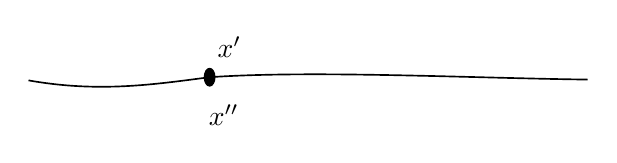
\begin{tikzpicture}[x=10mm,y=10mm]
\draw[line width=0.6pt] (0,0) .. controls (0.9,-0.16) and (1.6,-0.05) .. (2.3,0.04) .. controls (3.6,0.13) and (5.6,0.03) .. (7.1,0.01);
\path[fill=black] (2.3,0.04) ellipse[x radius=0.075,y radius=0.12];
\node at (2.55,0.42) {$x'$};\node at (2.48,-0.44) {$x''$};
\end{tikzpicture}\end{center}

\Unclear{GELFAND-P000099}{double-origin-diagram}{One nearly horizontal line with a thickened point; above it $x^{\prime}$, below it $x^{\prime\prime}$. Exact outline of the thickening undetermined.}
\end{GelfandAdjacentEvidence}
\begin{GelfandAdjacentEvidence}{GELFAND-P000099}{17}



\begin{tikzpicture}[baseline=0mm,x=1mm,y=1mm]
\path[fill=black] (0,0.6) -- (0.7,2.6) -- (5,2.6) -- (3.2,1.5) -- (6.6,1.5) -- (5.7,0) -- (1,0) -- cycle;
\draw[line width=0.7pt] (0,0.6) -- (0,-1);
\end{tikzpicture}\quad Check that the diag. is not closed.

\Unclear{GELFAND-P000099}{final-instruction}{Before Check, a separate dense black sign with two rightward projections; its role and exact outline undetermined. Check that the diag. is not closed.}
\end{GelfandAdjacentEvidence}





\begin{GelfandAdjacentEvidence}{GELFAND-P000100}{1}
\SourcePage{GELFAND-P000100}{unlabelled}

\underline{Classes of cycles modulo lin. equiv.}

\SourceFigure{GELFAND-P000100}{cycle-heading}{The entire heading Classes of cycles modulo lin. equiv. has a straight underline.}
\end{GelfandAdjacentEvidence}
\begin{GelfandAdjacentEvidence}{GELFAND-P000100}{2}


[a more precise inv. than cohom.)

\Unclear{GELFAND-P000100}{heading-aside}{A more precise inv. than cohom.; the opening bracket is angular, with a lower rightward foot, and its reading as [ / ( is not fully established; the closing parenthesis is round.}
\end{GelfandAdjacentEvidence}
\begin{GelfandAdjacentEvidence}{GELFAND-P000100}{3}


$X$ — an alg. variety, subvar. — a closed set in the top. of Zariski.

\SourceFigure{GELFAND-P000100}{variety-definition}{$X$ — an alg. variety; subvar. — a closed set in the top. of Zariski.}
\end{GelfandAdjacentEvidence}
\begin{GelfandAdjacentEvidence}{GELFAND-P000100}{4}


$V_i$ — subvarieties.

\SourceFigure{GELFAND-P000100}{subvariety-label}{$V_i$ — subvarieties; lower index $i$.}
\end{GelfandAdjacentEvidence}
\begin{GelfandAdjacentEvidence}{GELFAND-P000100}{5}



\begin{equation*}\sum\underset{\text{for.[?]}}{a_iV_i}\text{ — cycles}\qquad(a_i\text{ — integers})\end{equation*}

\Unclear{GELFAND-P000100}{formal-cycle}{Below the summand, the short source annotation for.[?] / form.[?]; after the distinct f-, o- and r-shaped letters, a cramped upper exit stroke. Formula $\sum a_iV_i$ and, at right, $(a_i\text{ — integers})$.}
\end{GelfandAdjacentEvidence}
\begin{GelfandAdjacentEvidence}{GELFAND-P000100}{6}


$\sum b_iU_i$. $2$ cycles are linearly equiv. if



$X\times P^1$\qquad in it there are subvar.\quad $\begin{gathered}X\times a,\\X\times b\\a,b\in P^1\end{gathered}$
\SourceFigure{GELFAND-P000100}{second-cycle}{$\sum b_iU_i$. $2$ cycles are linearly equiv. if; a period after $U_i$.}

\SourceFigure{GELFAND-P000100}{fiber-subvarieties}{$X\times P^1$; the words in it there are subvar.; at right $X\times a$, below it $X\times b$ and $a,b\in P^1$.}
\end{GelfandAdjacentEvidence}
\begin{GelfandAdjacentEvidence}{GELFAND-P000100}{7}


($P^1$ cov. by two ord. lines — an alg. var.)

\SourceFigure{GELFAND-P000100}{projective-cover}{($P^1$ cov. by two ord. lines — an alg. var.); the source abbreviation ob. and both parentheses.}
\end{GelfandAdjacentEvidence}
\begin{GelfandAdjacentEvidence}{GELFAND-P000100}{8}




\begin{tikzpicture}[baseline=0mm,x=1mm,y=1mm]
\path[fill=black] (0,0) -- (-0.5,2.1) -- (-0.9,3.6) -- (0.2,3.2) -- (0.4,4.6) -- (1.1,3.5) -- (1.8,4.3) -- (2,2.1) -- (2.6,1.7) -- (1.6,1.4) -- (1.7,0) -- (0.9,0.5) -- cycle;
\end{tikzpicture}\quad They are can. isom. to $X$.

\Unclear{GELFAND-P000100}{margin-star}{At left, a black vertical star-/letter-like mark with projections. Its approximate form is reproduced; letter reading and purpose undetermined.}

\SourceFigure{GELFAND-P000100}{canonical-isomorphism}{They are can. isom. to $X$.}
\end{GelfandAdjacentEvidence}
\begin{GelfandAdjacentEvidence}{GELFAND-P000100}{9}


$2$ cycles are equiv. if [crossed out: illegible] $\exists$ a $3$rd cycle, $W\text{[?]}\in X\times P^1$,
giving in intersect. with [crossed out: illegible] $X\times a$ the first, and
with $X\times b$ the second.

\Unclear{GELFAND-P000100}{cycle-equivalence-cancels}{After if, an expression with an initial v-like stroke is cancelled; after with, another word with a lower loop is cancelled. Full readings of the cancellations undetermined.}

\Unclear{GELFAND-P000100}{cycle-equivalence-body}{$\exists$ a $3$rd cycle, $W\text{[?]}\in X\times P^1$; the letter $W$[?] has cramped ascending strokes and may look N-like. A short lower comma follows cycle. The continuation with $X\times a$ and $X\times b$ occupies three lines.}
\end{GelfandAdjacentEvidence}
\begin{GelfandAdjacentEvidence}{GELFAND-P000100}{10}


\underline{Example.} $X$ — a surface, $U,V$ — curves.

\SourceFigure{GELFAND-P000100}{example-heading}{Example. is underlined including the period; $X$ — a surface, $U,V$ — curves.}
\end{GelfandAdjacentEvidence}
\begin{GelfandAdjacentEvidence}{GELFAND-P000100}{11}


They are lin. equiv. if $\exists$ [crossed-out sign illegible] a funct. with zeros
on $U$ and poles on $V$.

\Unclear{GELFAND-P000100}{rational-function-cancel}{Between the existence sign and funct., a small dense sign: a closed horizontal loop with a transverse stroke; letter reading undetermined.}

\SourceFigure{GELFAND-P000100}{linear-equivalence}{They are lin. equiv. if $\exists$ … a funct. with zeros on $U$ and poles on $V$.}
\end{GelfandAdjacentEvidence}
\begin{GelfandAdjacentEvidence}{GELFAND-P000100}{12}


Consider $X\times P^1$. Take in it $a=0$ and $b\mathrel{=\!\text{[?]}}\infty$.
In $X\times P^1$ take the cycle $(x,f(x))$

\Unclear{GELFAND-P000100}{graph-example}{Before $\infty$, after $b$, a dense short horizontal mark, $=$[?]; two separate bars cannot be distinguished confidently. On the next line, $(x,f(x))$: a tall $f$ stroke with a crossbar. The initial source Rassm. (Consider) has dense lower strokes; a separate underline is not established.}
\end{GelfandAdjacentEvidence}
\begin{GelfandAdjacentEvidence}{GELFAND-P000100}{13}


\underline{Def. of Chern[?] classes} (alg. varieties)

\Unclear{GELFAND-P000100}{chern-name-overwrite}{In the current word Chern[?], inner and final strokes are densely overwritten; earlier letters are not separable.}

\SourceFigure{GELFAND-P000100}{chern-heading}{A straight line runs under Def. of classes and the name Chern; at right, (alg. varieties).}
\end{GelfandAdjacentEvidence}
\begin{GelfandAdjacentEvidence}{GELFAND-P000100}{14}


They are giv. with fin.[?] axioms.

\Unclear{GELFAND-P000100}{axiom-abbreviation}{Before axioms, a short source kon.[?] / nek.[?], corresponding to fin.[?] / some[?]; cramped middle joins do not establish letter order.}

\SourceFigure{GELFAND-P000100}{axiom-phrase}{They are giv. with … axioms.; a period at the end of the line.}
\end{GelfandAdjacentEvidence}
\begin{GelfandAdjacentEvidence}{GELFAND-P000100}{15}


[Crossed-out initial sign illegible] Functor from the category [crossed-out circled sign illegible]

\Unclear{GELFAND-P000100}{category-cancellations}{At left before Functor, an earlier sign with a tall left stroke is densely cancelled; after category, another sign is cancelled and enclosed by a loop. Letter readings undetermined.}

\SourceFigure{GELFAND-P000100}{functor-line}{Functor from the category; separate cancellations at right and left.}
\end{GelfandAdjacentEvidence}
\begin{GelfandAdjacentEvidence}{GELFAND-P000100}{16}


Algebr. sheaf, algebr. $K$-functor.

\SourceFigure{GELFAND-P000100}{k-functor}{Algebr. sheaf, algebr. $K$-functor.}
\end{GelfandAdjacentEvidence}
\begin{GelfandAdjacentEvidence}{GELFAND-P000100}{17}


\hfill\begin{minipage}{0.52\linewidth}$A(X)$ —\\— gr. of lin. equiv.\\\hspace*{18mm}cycles\end{minipage}

\SourceFigure{GELFAND-P000100}{cycle-group}{At right $A(X)$ —; on the next line another dash before gr. of lin. equiv., with cycles below.}
\end{GelfandAdjacentEvidence}
\begin{GelfandAdjacentEvidence}{GELFAND-P000100}{18}


The map $K(X)\longrightarrow A(X)$ is linear.

\SourceFigure{GELFAND-P000100}{linear-map}{The map $K(X)\longrightarrow A(X)$ is linear.; an arrow directed to the right.}
\end{GelfandAdjacentEvidence}
\begin{GelfandAdjacentEvidence}{GELFAND-P000100}{19}


\underline{Axioms.}

\SourceFigure{GELFAND-P000100}{axiom-heading}{Axioms. has a straight underline.}
\end{GelfandAdjacentEvidence}
\begin{GelfandAdjacentEvidence}{GELFAND-P000100}{20}


1. [Crossed-out continuation illegible]

\Unclear{GELFAND-P000100}{first-axiom-cancel}{Final entry: 1. and a densely crossed-out line with two long transverse strokes. Below it, down to the lower edge, there are no further legible axioms.}
\end{GelfandAdjacentEvidence}




\begin{GelfandAdjacentEvidence}{GELFAND-P000101}{1}

\SourcePage{GELFAND-P000101}{67}
$18/\overline{\underline X}$. \underline{I.M. Gelfand.}
\par\hspace*{4mm}$X$

$E_1,\ldots,E_n$
\begin{equation*}
\Gamma(E_1)\overset d\longrightarrow\Gamma(E_2)
\overset d\longrightarrow\cdots\overset d\longrightarrow\Gamma(E_n)
\end{equation*}
[Crossed out at right: Diff.[?] oper.[?]] Ell. complex.
\Unclear{GELFAND-P000101}{top-cancellations}{Two densely crossed-out entries: Diff.[?] / Differ.[?] and oper.[?]. The distinct remnants do not establish all cancelled letters.}
\end{GelfandAdjacentEvidence}
\begin{GelfandAdjacentEvidence}{GELFAND-P000101}{2}

\begin{equation*}
d\bigl(f^m(x)s(x)\bigr)\big|_{x_0}=\sigma(d,\eta)s(x_0),
\qquad df\big|_{x_0}=\eta
\end{equation*}
$\sigma$ — symbol of the diff. oper.
\begin{equation*}
0\longrightarrow E_{1,x_0}\underset{\sigma(d,\eta)}\longrightarrow E_{2,x_0}
\longrightarrow\cdots\overset{\sigma(d,\eta)}\longrightarrow E_{n,x_0}\longrightarrow0.
\end{equation*}
\SourceFigure{GELFAND-P000101}{symbol-sequence-placement}{At the first arrow between fibres, $\sigma(d,\eta)$ is below; at the last, above; zeros at both ends.}
\end{GelfandAdjacentEvidence}
\begin{GelfandAdjacentEvidence}{GELFAND-P000101}{3}

\underline{Map.} $T:\Gamma(E)\longrightarrow\Gamma(E)$.
\hfill$\Gamma(E_i)\longrightarrow\Gamma(E_i)$

$f:X\longrightarrow X$

$\varphi$ induc.[?] bundle.
\Unclear{GELFAND-P000101}{bundle-contraction}{Between $\varphi$ and bundle, the connected source abbreviation induc.[?] / endom.[?]; the first letter is densely overwritten, with a tall middle stroke and an upper arch.}
\end{GelfandAdjacentEvidence}
\begin{GelfandAdjacentEvidence}{GELFAND-P000101}{4}


\begin{center}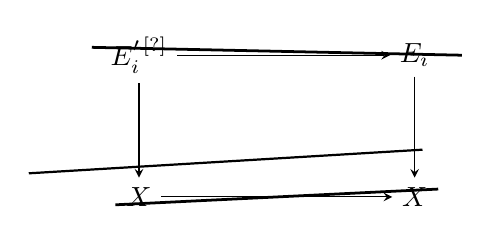
\begin{tikzpicture}[x=1mm,y=1mm,>=stealth]
\node(a)at(0,18){$E_i^{\prime\,[?]}$};\node(b)at(35,18){$E_i$};
\node(c)at(0,0){$X$};\node(e)at(35,0){$X$};
\draw[->](a)--(b);\draw[->](a)--(c);\draw[->](b)--(e);\draw[->](c)--(e);
\draw[line width=1pt](-6,19)--(41,18);
\draw[line width=.8pt](-14,3)--(36,6);
\draw[line width=1pt](-3,-1)--(38,1);
\end{tikzpicture}\end{center}

\Unclear{GELFAND-P000101}{cancelled-bundle-square}{Crossed-out square: upper $E_i$ labels, with a possible added upper stroke at left; rightward and downward arrows, $X\to X$ below. Several long cancellation strokes; exact hidden indices and outlines undetermined.}
\end{GelfandAdjacentEvidence}
\begin{GelfandAdjacentEvidence}{GELFAND-P000101}{5}


\begin{center}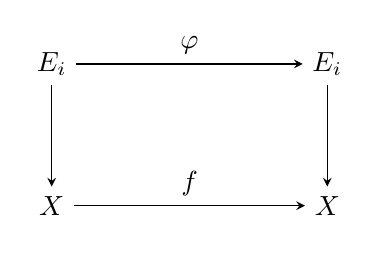
\begin{tikzpicture}[x=1mm,y=1mm,>=stealth]
\node(a)at(0,18){$E_i$};\node(b)at(35,18){$E_i$};
\node(c)at(0,0){$X$};\node(e)at(35,0){$X$};
\draw[->](a)--node[above]{$\varphi$}(b);\draw[->](a)--(c);
\draw[->](b)--(e);\draw[->](c)--node[above]{$f$}(e);
\end{tikzpicture}\end{center}

\SourceFigure{GELFAND-P000101}{active-bundle-square}{Upper arrow $E_i\overset\varphi\longrightarrow E_i$, two downward arrows; lower arrow $X\overset f\longrightarrow X$.}
\end{GelfandAdjacentEvidence}
\begin{GelfandAdjacentEvidence}{GELFAND-P000101}{6}

(In the simplest cases $\varphi$ determines $f$ —
— forms $f$ determ. the map of tang. vectors)

Endom., if it commut. with $d$.

$T$ is an oper. in a $C^\infty$-space. The theorem reduces to the study of the trace
(it is calc. in $2$ ways)

\underline{Theorem 1.} The complex has finite
[crossed-out word illegible] homologies.
\Unclear{GELFAND-P000101}{theorem-cancel}{Between finite and homologies, a word is densely crossed out; an upper arch and a lower stroke remain. Full reading undetermined.}
\end{GelfandAdjacentEvidence}
\begin{GelfandAdjacentEvidence}{GELFAND-P000101}{7}


Let $\omega^n$ be a form of ord. $n$ on $X$, not taking the value $0$.
Use it to introduce a Hermitian structure. (Let it
exist once and for all. \underline{Noninv}ariant, but simpler.)
\begin{equation*}
\int\langle s,\alpha(s')\rangle=\int_X\overline{(s,s')}\,\omega.
\end{equation*}
\SourceFigure{GELFAND-P000101}{hermitian-pairing}{At left, angle brackets containing $s,\alpha(s')$; at right, integral over $X$, a bar over $(s,s')$, then $\omega$.}
\end{GelfandAdjacentEvidence}
\begin{GelfandAdjacentEvidence}{GELFAND-P000101}{8}

\begin{equation*}d^*\underset{\mathrm{def}}{=}\alpha^{-1}\cdot d'\circ\alpha.\end{equation*}
\Unclear{GELFAND-P000101}{adjoint-definition}{The top of the initial $d$ is dense, with a star beside it. Below the equality, def; at right $\alpha^{-1}\cdot d'\circ\alpha$. No separate sign is securely readable inside the dense part.}
\end{GelfandAdjacentEvidence}
\begin{GelfandAdjacentEvidence}{GELFAND-P000101}{9}

$s\in\Gamma(E)$, $s'\in\Gamma_c(E')$.
\Unclear{GELFAND-P000101}{dual-section-index}{The lower part of the first $\Gamma$ is overwritten; the second $\Gamma$ has an open lower loop, read as $c$, possibly o-like.}
\end{GelfandAdjacentEvidence}
\begin{GelfandAdjacentEvidence}{GELFAND-P000101}{10}


$E'$ — the dual sheaf.
\begin{equation*}\Box\underset{\mathrm{def}}{=}d^*d+dd^*\end{equation*}
[A separate black mark below and to the left of the definition.]
\Unclear{GELFAND-P000101}{middle-ink-mark}{A separate dense blot with small dots and slanting strokes; letter reading and purpose undetermined.}
\end{GelfandAdjacentEvidence}
\begin{GelfandAdjacentEvidence}{GELFAND-P000101}{11}

($d'$ — simply the adjoint operator)

$\Box$ — an ellipt. operator, taking each $\Gamma(E_i)$ into itself.

$\Gamma_\lambda(E)$ — sections satisfying the eqn. $\Box s=\lambda s$.
Since $\Box$ is elliptic, for $\forall\lambda$ a fin. number of distinct lin. indep. eig. functs.
[dense separate sign illegible].
\Unclear{GELFAND-P000101}{eigenfunction-end-sign}{After eig. functs., a separate dense closed black entry with inner vertical strokes; an H-like reading is not established.}
\end{GelfandAdjacentEvidence}
\begin{GelfandAdjacentEvidence}{GELFAND-P000101}{12}

\begin{equation*}\Box d=d\Box\end{equation*}
\begin{equation*}
\Gamma_\lambda(E_1)\overset d\longrightarrow\Gamma_\lambda(E_2)
\overset d\longrightarrow\cdots\longrightarrow\Gamma_\lambda(E_n)
\end{equation*}
\SourceFigure{GELFAND-P000101}{lower-sequence-punctuation}{The second closing parenthesis has a low outgoing stroke touching the next line; no separate comma established.}
\end{GelfandAdjacentEvidence}
\begin{GelfandAdjacentEvidence}{GELFAND-P000101}{13}

Introduce the homology groups
[below, crossed-out formula illegible].
\Unclear{GELFAND-P000101}{homology-cancel}{Below homology groups, two long transverse strokes cross a short formula; upright bases and an upper slanting stroke remain. Full reading undetermined.}
\end{GelfandAdjacentEvidence}
\begin{GelfandAdjacentEvidence}{GELFAND-P000101}{14}


\begin{center}\begin{tikzpicture}[x=1mm,y=1mm]
\node[anchor=west](h)at(0,7){$H^i(\Gamma_\lambda(E))=\operatorname{Ker}d\big|_{\Gamma_{\lambda\text{[?]}}(E_i)}$};
\draw[line width=.6pt](110,-9)--(127,12);
\node[anchor=west](den)at(115,-8){$\operatorname{Im}d\text{[?]}$};
\draw[line width=.8pt](115,-8)--(132,-7);
\node[anchor=west]at(136,-8){$\ldots$};
\end{tikzpicture}\end{center}

\Unclear{GELFAND-P000101}{kernel-restriction}{After the vertical bar, $\Gamma$ with a dense lower sign $\lambda$[?], then $(E_i)$; the initial Ker has a capital K.}
\end{GelfandAdjacentEvidence}
\begin{GelfandAdjacentEvidence}{GELFAND-P000101}{15}

\Unclear{GELFAND-P000101}{homology-denominator}{At right a slanting quotient stroke; below, densely crossed-out $\operatorname{Im}d$[?], then three separate dots. The cancelled middle strokes remain unread.}
\end{GelfandAdjacentEvidence}
\begin{GelfandAdjacentEvidence}{GELFAND-P000102}{16}



\SourcePage{GELFAND-P000102}{unlabelled}
Without proof this work asserts Hodge's theorem
\begin{equation*}
H^i(\Gamma_\lambda(E))^{*\text{[?]}}=
\begin{cases}H^i(E)&\lambda=0\\0&\lambda\ne0.\end{cases}
\end{equation*}
\Unclear{GELFAND-P000102}{complex-star}{Above the right closing parentheses, a small dense star-like mark; its exact attachment to the parentheses and notation is undetermined.}
\end{GelfandAdjacentEvidence}
\begin{GelfandAdjacentEvidence}{GELFAND-P000102}{17}

\uwave{Dynin.} For $\lambda\ne0$ — here $0$.
($d$ for $\lambda\ne0$ maps eig. functs.
[crossed-out word illegible] exact compl.
\Unclear{GELFAND-P000102}{dynin-cancel}{Before exact compl., a short entry is densely crossed out. After it, exact compl.; the final source letters are cramped, with a separate arch above them. The cancelled letters remain unread.}
\end{GelfandAdjacentEvidence}
\begin{GelfandAdjacentEvidence}{GELFAND-P000102}{18}


\begin{center}\begin{tikzpicture}
\node[inner sep=2mm](k){$H^i(\Gamma_\lambda(E))=\operatorname{Ker}(\Box-\lambda)$};
\draw[line width=.5pt]([xshift=-2mm,yshift=1mm]k.south west)
 --([xshift=-2mm,yshift=-2mm]k.south west)
 --([xshift=2mm,yshift=-2mm]k.south east)
 --([xshift=2mm,yshift=1mm]k.south east);
\end{tikzpicture}\end{center}

this is Hodge's theor. $\forall\lambda$
\SourceFigure{GELFAND-P000102}{dynin-kernel-claim}{Three sides of a frame below the formula and at both edges, open at the top. At right $\operatorname{Ker}(\Box-\lambda)$, with an initial capital K.}
\end{GelfandAdjacentEvidence}
\begin{GelfandAdjacentEvidence}{GELFAND-P000102}{19}

($\forall$ ell. oper. $\underset{?}{\text{[crossed out: illegible]}}$
$\Box-\lambda$ — a new letter, again Hodge's theor.\ldots
\Unclear{GELFAND-P000102}{dynin-general-cancel}{After ell. oper., a short abbreviation is densely cancelled; a question mark lies immediately below it. Full reading undetermined.}
\end{GelfandAdjacentEvidence}
\begin{GelfandAdjacentEvidence}{GELFAND-P000102}{20}

\SourceFigure{GELFAND-P000102}{dynin-parentheses}{Visible opening round parentheses before $d$ and before $\forall$ ell. oper.; the last line has three separate dots after Hodge. No closing parentheses read in this fragment.}
\end{GelfandAdjacentEvidence}
\begin{GelfandAdjacentEvidence}{GELFAND-P000102}{21}


\uwave{Bernstein.} Same. $H^i(\Gamma_\lambda(E))=0$, $\lambda\ne0$.
Let $s\in\Gamma_\lambda(E_i)$ and let $ds=0$.
[?] $\Box s=dd^*s$. Then $\lambda s=d(d^*s)$
and $s=d\left(\frac{d^*s}{\lambda}\right)$,
$d^*s$ is an eig. funct. ($d^*$ commut. with $\Box$).
\Unclear{GELFAND-P000102}{bernstein-square-prefix}{Before $\Box$, a tall dense stroke with a closed upper loop and a lower slanting exit: $d$[?] / opening parenthesis[?]. Reading undetermined.}
\end{GelfandAdjacentEvidence}
\begin{GelfandAdjacentEvidence}{GELFAND-P000102}{22}

\SourceFigure{GELFAND-P000102}{bernstein-division}{The entry $s=d\left(\frac{d^*s}{\lambda}\right)$: a long horizontal bar passes near the base of the outer $d$ and across the parentheses; a separate comma at right.}
\end{GelfandAdjacentEvidence}
\begin{GelfandAdjacentEvidence}{GELFAND-P000102}{23}


$d^*s\in C^\infty$ follows from the \underline{theor.} on \underline{ell.} eqns.
\underline{Gelfand again.}
For $\lambda=0$ transfer Hodge's proof literally.
\SourceFigure{GELFAND-P000102}{source-emphasis}{Wavy lines below Dynin. and Bernstein.; a straight line below Gelfand again. In the line before the last heading, theor. and ell. are separately underlined.}
\end{GelfandAdjacentEvidence}
\begin{GelfandAdjacentEvidence}{GELFAND-P000102}{24}

\begin{equation*}\Gamma(E)=\sum\Gamma_\lambda(E)\qquad(\text{discr. spectrum})\end{equation*}
\SourceFigure{GELFAND-P000102}{spectral-decomposition}{$\Gamma(E)=\sum\Gamma_\lambda(E)$; no separate index visible below the summation sign.}
\end{GelfandAdjacentEvidence}
\begin{GelfandAdjacentEvidence}{GELFAND-P000102}{25}

Besides the oper. $T$, introduce
\begin{equation*}\fbox{$T_\lambda=\pi_\lambda\circ T\circ i_\lambda,$}\end{equation*}
where $i_\lambda:\Gamma_\lambda(E)\longrightarrow\Gamma(E)$,
$\pi_\lambda:\Gamma(E)\longrightarrow\Gamma_\lambda(E)$ — orthog. projection.
\SourceFigure{GELFAND-P000102}{projected-operator}{Rectangular frame around $T_\lambda=\pi_\lambda\circ T\circ i_\lambda$; a final comma inside the frame. Below, the line with $\pi_\lambda$ and orthog. projection; above the frame (discr. spectrum).}
\end{GelfandAdjacentEvidence}
\begin{GelfandAdjacentEvidence}{GELFAND-P000102}{26}


(oper. $T$ in this cell) Lefschetz number for $T$.

$T$ — a map of sections, thus a map of sections $\Gamma(E)\to\Gamma(E)$
\begin{equation*}L(T,E)=\sum(-1)^i\operatorname{tr}(T_i^*|H_i\text{[?]}).\end{equation*}
\Unclear{GELFAND-P000102}{lefschetz-space}{After the vertical bar, an H-like letter is densely overwritten; a separate $i$ lies at the lower right, with a dot above it. The main letter and index placement remain uncertain: $H_i$[?] / $H^i$[?].}
\end{GelfandAdjacentEvidence}
\begin{GelfandAdjacentEvidence}{GELFAND-P000102}{27}

By Hodge's theor. $T_{\lambda=0}=T^*$.
\hfill$\Pi_0\text{[?]}=T^{*\text{[?]}}$
\Unclear{GELFAND-P000102}{hodge-stars}{At left $T_{\lambda=0}=T^*$. At right, the first letter has a long top bar and a lower $0$: $\Pi_0$[?] / $\pi_0$[?] / $T_0$[?]. Above the right $T$, a dense star-like entry; one or two overlapping stars cannot be distinguished securely.}
\end{GelfandAdjacentEvidence}
\begin{GelfandAdjacentEvidence}{GELFAND-P000102}{28}

\begin{gather*}
\sum(-1)^i\operatorname{tr}(T_0|E_i)=L(T,E)\\
\sum(-1)^i\operatorname{tr}(T_\lambda|E_i)=0\qquad\lambda\ne0
\end{gather*}
[At right, two densely crossed-out entries illegible.]
\Unclear{GELFAND-P000102}{right-cancellations}{Two small dense cancellations in the right margin: the upper one has a lower loop, the lower a long rising slanting stroke. Letter readings undetermined.}
\end{GelfandAdjacentEvidence}
\begin{GelfandAdjacentEvidence}{GELFAND-P000102}{29}


(the trace in hom. is the same as the trace in the spaces themselves)

(By Hodge's theor. $H^i(E)=\Gamma_0(E_i)$)
\begin{equation*}\Box s=0\Longrightarrow\underline{ds=0}.\end{equation*}
\SourceFigure{GELFAND-P000102}{zero-hodge-implication}{In $\Box s=0\Longrightarrow ds=0$, a thick overwritten arrow; below $ds=0$, a horizontal line, with a separate dot at right.}
\end{GelfandAdjacentEvidence}
\begin{GelfandAdjacentEvidence}{GELFAND-P000102}{30}

(from immed.[?] def. and so on)
\Unclear{GELFAND-P000102}{positive-aside}{After from, a dense connected source abbreviation neposr. (immed.)[?] / polozh. (positive)[?]; at right def. and so on, then a closing round parenthesis. Dense overwriting above the early middle strokes.}
\end{GelfandAdjacentEvidence}
\begin{GelfandAdjacentEvidence}{GELFAND-P000102}{31}


Must give meaning to $\sum(-1)^i\operatorname{tr}(T|E_i)$. Regulariz. it.
\par In $2$ ways.
\SourceFigure{GELFAND-P000102}{regularization-order}{First line: Must give meaning, the sum, and Regulariz. it at right. Below at left: In $2$ ways.}
\end{GelfandAdjacentEvidence}
\begin{GelfandAdjacentEvidence}{GELFAND-P000103}{32}



\SourcePage{GELFAND-P000103}{68}
In finite $\Gamma_\lambda(E)$
\begin{equation*}d:\Gamma_\lambda(E_1)\longrightarrow\Gamma_\lambda(E_2)\longrightarrow\cdots\end{equation*}
(finite-dimensionality)
$T$ — its map into itself. Then
\begin{equation*}\sum(-1)^i\operatorname{tr}T|_{E_i}=\sum(-1)^i\operatorname{tr}T|_{H_i}\end{equation*}
(and $H^i=0$)
\par(invar. of the Euler characteristic)
\SourceFigure{GELFAND-P000103}{finite-trace-complex}{The first chain has two arrows, then an ellipsis; finite-dimensionality in parentheses. In the trace equality, $E_i$ and $H_i$ have subscripts after the restriction bars; the next parenthesis has $H^i=0$ with superscript i.}
\end{GelfandAdjacentEvidence}
\begin{GelfandAdjacentEvidence}{GELFAND-P000103}{33}


Consider.
\begin{equation*}\sum_\lambda(1+\lambda)^{-z}\operatorname{tr}(T_\lambda|E_i)=\operatorname{tr}^{z}(E_i)\end{equation*}
\underline{Theorem.} The series conv. for $\operatorname{Re}z>\frac12\dim X$
(on the asympt. of eig. functions) (Dunford and Schwartz, vol.2)
\par This is an anal. funct. of $z$ in the half-plane.
\SourceFigure{GELFAND-P000103}{regularized-trace}{The exponent of $(1+\lambda)$ is $-z$, with a separate short minus stroke. At right, $\operatorname{tr}^{z}(E_i)$. Beneath, Theorem. is underlined; $\operatorname{Re}z>\frac12\dim X$ and two parentheses.}
\end{GelfandAdjacentEvidence}
\begin{GelfandAdjacentEvidence}{GELFAND-P000103}{34}

\begin{equation*}L(T,E)=\sum(-1)^i\operatorname{tr}^{z}E_i\qquad\forall z\end{equation*}
\SourceFigure{GELFAND-P000103}{all-z-identity}{At left, $L(T,E)$; at right the trace has superscript z, then $E_i$ without parentheses. Farther right, a separate $\forall z$ with a dense first sign.}
\end{GelfandAdjacentEvidence}
\begin{GelfandAdjacentEvidence}{GELFAND-P000103}{35}

(everything except convergence is proved [densely overwritten sign illegible]

---
\begin{center}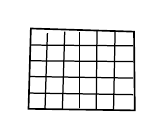
\begin{tikzpicture}[x=1cm,y=1cm]
\draw[line width=.6pt](0,0)--(1.35,-.02)--(1.34,.98)--(.03,1.02)--cycle;
\draw[line width=.45pt](.21,.01)--(.24,.96);
\draw[line width=.45pt](.43,-.01)--(.46,.98);
\draw[line width=.45pt](.65,.01)--(.65,.98);
\draw[line width=.45pt](.86,-.01)--(.87,.99);
\draw[line width=.45pt](1.08,-.01)--(1.10,.99);
\draw[line width=.45pt](.02,.20)--(1.33,.18);
\draw[line width=.45pt](.01,.41)--(1.33,.39);
\draw[line width=.45pt](.02,.61)--(1.33,.60);
\draw[line width=.45pt](.02,.81)--(1.33,.80);
\end{tikzpicture}\end{center}
)
\Unclear{GELFAND-P000103}{proof-overwrite}{After proved, a dense vertical entry with a lower oblique looplike exit. Former letters remain inseparable even under enlargement; exact reading undetermined.}
\end{GelfandAdjacentEvidence}
\begin{GelfandAdjacentEvidence}{GELFAND-P000103}{36}

\SourceFigure{GELFAND-P000103}{proof-grid}{After the dash, a small rectangular grid of horizontal and vertical strokes. The typographic recreation shows the visible lines; dense intersections and borders are not fully distinguishable. No letter label or definite role of the grid is read.}
\end{GelfandAdjacentEvidence}
\begin{GelfandAdjacentEvidence}{GELFAND-P000103}{37}



Since $T\sim$ is bounded (asympt. of eig. functions)
\par(on anal. cont., a pole at $z=0$)
\SourceFigure{GELFAND-P000103}{bounded-tilde}{After T, a separate wavy $\sim$ sign, then bounded; asympt. of eig. functions in parentheses. Beneath, a separate parenthesis: on anal. cont., a pole at $z=0$.}
\end{GelfandAdjacentEvidence}
\begin{GelfandAdjacentEvidence}{GELFAND-P000103}{38}


\underline{Example.} $S^1$
\begin{center}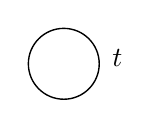
\begin{tikzpicture}[x=1cm,y=1cm]
\draw[line width=.5pt](0,0)circle(.45);
\node at(.68,.08){$t$};
\end{tikzpicture}\end{center}
$d=\frac d{dt}$, ell. oper., $\Box=\frac{d^2}{dt^2}$.
\SourceFigure{GELFAND-P000103}{circle-derivative}{A circle with t at right. The initial d in the first derivative's denominator is densely overwritten, followed by t; former strokes are inseparable. The entry for $\Box$ is $d^2/dt^2$ with a positive sign.}
\end{GelfandAdjacentEvidence}
\begin{GelfandAdjacentEvidence}{GELFAND-P000103}{39}


$T=(f,\varphi)$,
\begin{gather*}dS(x)=s(x)\\Ts(x)=\varphi(x)s(f(x))\end{gather*}
\SourceFigure{GELFAND-P000103}{section-equations}{At left, $T=(f,\varphi)$ and a comma. At upper right, $dS(x)=s(x)$: the first S is uppercase, the second s lowercase. Beneath, $Ts(x)=\varphi(x)s(f(x))$.}
\end{GelfandAdjacentEvidence}
\begin{GelfandAdjacentEvidence}{GELFAND-P000103}{40}

\begin{center}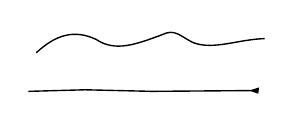
\begin{tikzpicture}[x=1cm,y=1cm]
\draw[line width=.5pt](0,.55)..controls(.25,.78)and(.48,.85)..(.76,.72)
 ..controls(1,.56)and(1.25,.65)..(1.60,.78)
 ..controls(1.76,.86)and(1.83,.76)..(1.99,.68)
 ..controls(2.25,.58)and(2.56,.72)..(2.90,.73);
\draw[line width=.5pt](-.10,.06)--(.62,.08)--(1.47,.06)--(2.72,.07);
\path[fill=black](2.70,.07)--(2.83,.11)--(2.82,.03)--cycle;
\end{tikzpicture}\end{center}
\SourceFigure{GELFAND-P000103}{small-wave}{At left beneath $T=(f,\varphi)$, a separate wavy line; below it, an almost horizontal stroke with a thickened right end. The typographic recreation preserves the general course of the lines; direction of the thickening and purpose of the sketch are undetermined. There are no axis or function labels.}
\end{GelfandAdjacentEvidence}
\begin{GelfandAdjacentEvidence}{GELFAND-P000103}{41}


\underline{Definition} [?] of a pseudodiff. oper.:
\Unclear{GELFAND-P000103}{definition-prefix}{Between the heading and pseudodiff., a dense overwritten sign with a right vertical and several transverse strokes: P[?] / illegible. No secure letter reading established.}
\end{GelfandAdjacentEvidence}
\begin{GelfandAdjacentEvidence}{GELFAND-P000103}{42}

$X$ — manifold. $\Gamma(E)$, $\Gamma(F)$ — 2 bundles on $X$
\begin{equation*}P:\Gamma_c(E)\longrightarrow\Gamma(F)\end{equation*}
$\Gamma_c(E)$ — sections with compact support.
[Crossed out: Called[?]]
\Unclear{GELFAND-P000103}{pseudo-cancel}{Before Lin. oper. is called, a short abbreviation with a long lower oblique cancellation stroke. Source Naz.[?] (Called[?]); former letters are densely joined and not securely read. A separate period follows.}
\end{GelfandAdjacentEvidence}
\begin{GelfandAdjacentEvidence}{GELFAND-P000103}{43}

A lin. oper. is called pseudodiff. if $\exists$ a seq. of numbers
$n_1>n_2>n_3>\cdots\to-\infty$

and satisfies the following conditions
\begin{equation*}e^{-i\lambda g}\underline{P}(e^{i\lambda g}s)\end{equation*}
$g\in\Gamma(1)$ ($C^\infty$ funct.),
1 — trivial sheaf, $s(x)\in\Gamma_c(E)$, $dg\ne0$ on $\operatorname{supp}s$,
if there is an asympt. expansion.




\SourcePage{GELFAND-P000104}{unlabelled}
\begin{equation*}\sim\sum_0^\infty P_j(s,g)\lambda^{n_j}\end{equation*}
\Unclear{GELFAND-P000103}{order-signs}{Three right-pointing signs. The first and third have dense lower ends and separate tiny traces; the middle one is overwritten and joins the following n. Separate lower equality strokes are not established: $>$[?] / $\geq$[?].}
\end{GelfandAdjacentEvidence}
\begin{GelfandAdjacentEvidence}{GELFAND-P000103}{44}

\SourceFigure{GELFAND-P000103}{pseudo-definition}{The heading Definition has a straight underline. In the exponential expression, P has a short underline; exponents $-i\lambda g$ and $i\lambda g$. In parentheses, $C^\infty$ funct. At right, $dg\ne0$; beneath, on $\operatorname{supp}s$ and a comma.}
\end{GelfandAdjacentEvidence}
\begin{GelfandAdjacentEvidence}{GELFAND-P000103}{45}

\Unclear{GELFAND-P000103}{bottom-mark}{To the right of asympt. expansion., a short dense isolated mark: an upper loop, a horizontal exit to the right and a lower projection. Letter reading and association undetermined.}
\end{GelfandAdjacentEvidence}
\begin{GelfandAdjacentEvidence}{GELFAND-P000104}{46}


\SourceFigure{GELFAND-P000104}{asymptotic-continuation}{Continuation of the formula: a separate $\sim$, lower limit $0$ without $j=$, upper $\infty$, then $P_j(s,g)\lambda^{n_j}$.}
\end{GelfandAdjacentEvidence}
\begin{GelfandAdjacentEvidence}{GELFAND-P000104}{47}


$26/\underline{\overline{X}}$ \underline{Continuation.} Ell. complex.
\SourceFigure{GELFAND-P000104}{continuation-header}{X in the date has separate over- and underlines. Continuation. has its own underline; then Ell. complex.}
\end{GelfandAdjacentEvidence}
\begin{GelfandAdjacentEvidence}{GELFAND-P000104}{48}

In $E_i$ — a Hermitian metric, and in $X$ — integration.
Introduce oper. $d^*$, $\Box=dd^*+d^*d$, $\Box d=d\Box$
\par $\Box s=\lambda s$, $\Box$ self-adj. and positive, elliptic, $\lambda>0$.
$\Box s=0\Longrightarrow ds=0$
\begin{equation*}d\Gamma_\lambda(E_i)\subset\Gamma_\lambda(E_{i+1})\end{equation*}
\Unclear{GELFAND-P000104}{laplacian-commutation-edge}{At right in $\Box d=d\Box$, the last square's right edge is broken and faint. Its other sides are distinguishable; the exact right boundary of the sign is damaged in the held scan. Beneath, separate entries $\lambda>0$ and $\Box s=0\Longrightarrow ds=0$.}
\end{GelfandAdjacentEvidence}
\begin{GelfandAdjacentEvidence}{GELFAND-P000104}{49}


\begin{equation*}0\overset{d}{\longrightarrow}\Gamma(E)\overset{d}{\longrightarrow}\Gamma(F)\overset{d}{\longrightarrow}0\end{equation*}
$d$ — simply an elliptic operator, $ds=0$ — the kernel.
Image $s_1=ds_*$,
\Unclear{GELFAND-P000104}{image-preimage}{The first s has a lower sign resembling $1$, possibly $i$. The star-like sign after the second s lies close to the baseline; its height is ambiguous: $s_1=ds_*$ / $s_i=ds^*$ / illegible index.}
\end{GelfandAdjacentEvidence}
\begin{GelfandAdjacentEvidence}{GELFAND-P000104}{50}

\uwave{Homology:} $\operatorname{Ker}d|_E$, $\operatorname{Coker}d|_F$.
The Lefschetz number — the \underline{index}
\SourceFigure{GELFAND-P000104}{two-term-homology}{All three arrows of the first chain are labelled d. Homology: has a wavy underline; Ker and Coker begin with capitals. Index has a separate straight underline.}
\end{GelfandAdjacentEvidence}
\begin{GelfandAdjacentEvidence}{GELFAND-P000104}{51}


\begin{equation*}\Gamma_\lambda(E_i)\overset{d}{\longrightarrow}\Gamma_\lambda(E_{i+1})\longrightarrow\cdots\end{equation*}
already a finite-dimensional complex,
its hom. $=0$ for $\lambda\ne0$ and $=H^i$
[crossed out: for] [illegible phrase]
for $\lambda=0$.
\Unclear{GELFAND-P000104}{zero-cohomology-words}{After $H^i$, the source word при (for) is densely crossed out. Then joined loops: самое конеч.[?] (most finite.[?]) / само конеч.[?] (itself finite.[?]); the first word is not securely read. Finally, for $\lambda=0$.}
\end{GelfandAdjacentEvidence}
\begin{GelfandAdjacentEvidence}{GELFAND-P000104}{52}


$T_i^*\quad H^i$
\begin{equation*}\sum(-1)^i\operatorname{tr}(T_i^*)=L(T,E)\end{equation*}
Compute through fixed points.
\par $T$ — a map of $X$, commutes with $d$.
\SourceFigure{GELFAND-P000104}{lefschetz-actions}{At left, separate $T_i^*$ and $H^i$, without an arrow between them. At right, an equality with $L(T,E)$. Beneath, T — a map of X, commutes with d.; at right, Compute through fixed points.}
\end{GelfandAdjacentEvidence}
\begin{GelfandAdjacentEvidence}{GELFAND-P000104}{53}


$T$ is a map of $\Gamma_\lambda(E_i)$
Introd. operators $\pi_\lambda$ and $i_\lambda$.
inclusion of $\Gamma_\lambda$ into all of $\Gamma$, and projection onto
[crossed out: illegible entry]

$\Gamma_\lambda(E_i)$.
\Unclear{GELFAND-P000104}{projection-cancel}{After onto, a short densely cancelled entry with an upper loop and transverse strokes. Former letters remain inseparable; followed by a separate active $\Gamma_\lambda(E_i)$.}
\end{GelfandAdjacentEvidence}
\begin{GelfandAdjacentEvidence}{GELFAND-P000104}{54}


\begin{equation*}T_\lambda=\pi_\lambda\cdot T i_\lambda\end{equation*}
(select the blocks corresp. to $\Gamma_\lambda$)
\SourceFigure{GELFAND-P000104}{projection-definition}{Entries for inclusion of $\Gamma_\lambda$ into all of $\Gamma$ and projection onto $\Gamma_\lambda(E_i)$. The formula has one multiplication dot before T; no separate dot between T and $i_\lambda$. Beneath, a parenthesis about selecting blocks.}
\end{GelfandAdjacentEvidence}
\begin{GelfandAdjacentEvidence}{GELFAND-P000104}{55}


Commut. unnecessary, suff.
[dense overwritten sign]

\begin{center}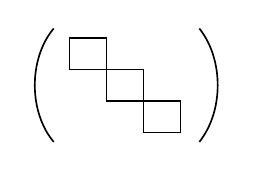
\begin{tikzpicture}[x=1cm,y=1cm]
\draw[line width=.6pt](0,0)--(.47,0)--(.47,-.40)--(0,-.40)--cycle;
\draw[line width=.6pt](.47,-.40)--(.94,-.40)--(.94,-.80)--(.47,-.80)--cycle;
\draw[line width=.6pt](.94,-.80)--(1.41,-.80)--(1.41,-1.20)--(.94,-1.20)--cycle;
\draw[line width=.6pt](-.20,.12)..controls(-.52,-.26)and(-.52,-.94)..(-.20,-1.32);
\draw[line width=.6pt](1.65,.12)..controls(1.96,-.27)and(1.96,-.93)..(1.65,-1.32);
\end{tikzpicture}\end{center}
in the blocks.
\Unclear{GELFAND-P000104}{cell-cancel}{Between suff. and the sketch, a dense vertical entry with two dark clusters and a lower oblique exit. No letter reading established; the sign is retained separately from the blocks.}
\end{GelfandAdjacentEvidence}
\begin{GelfandAdjacentEvidence}{GELFAND-P000104}{56}


\SourceFigure{GELFAND-P000104}{diagonal-cells}{Three empty squares descend from upper left to lower right within parentheses; neighbouring corners touch. The typographic recreation preserves the three outlines and parentheses; exact sizes and dense joints remain undetermined.}
\end{GelfandAdjacentEvidence}
\begin{GelfandAdjacentEvidence}{GELFAND-P000104}{57}


Then \fbox{$T^*=T_0$}
\begin{equation*}0\longrightarrow\Gamma_0(E_1)\overset{d}{\longrightarrow}\Gamma_0(E_2)\overset{d}{\longrightarrow}\cdots\end{equation*}
all $d=0$ since $\Box s=0$.
\SourceFigure{GELFAND-P000104}{zero-complex-frame}{The equality $T^*=T_0$ has a full rectangular frame. The first arrow from 0 is unlabelled, the next two have d; then an ellipsis. At right, all $d=0$; beneath, since $\Box s=0$.}
\end{GelfandAdjacentEvidence}
\begin{GelfandAdjacentEvidence}{GELFAND-P000104}{58}


All homology in $\Gamma_0$
\begin{center}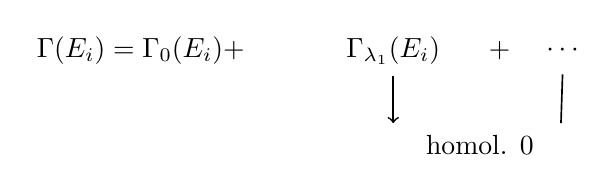
\begin{tikzpicture}[x=1cm,y=1cm]
\node[anchor=west]at(0,0){$\Gamma(E_i)=\Gamma_0(E_i)+$};
\node at(4.65,0){$\Gamma_{\lambda_1}(E_i)$};
\node at(6.00,0){$+$};\node at(6.80,0){$\cdots$};
\draw[line width=.6pt,->](4.65,-.32)--(4.65,-.92);
\draw[line width=.6pt](6.80,-.30)--(6.78,-.92);
\node at(5.75,-1.20){homol. $0$};
\end{tikzpicture}\end{center}
\SourceFigure{GELFAND-P000104}{decomposition-arrows}{A short downward arrow beneath $\Gamma_{\lambda_1}(E_i)$; a separate vertical stroke with a dense lower end beneath the ellipsis. Beneath, homol. 0. No arrow beneath $\Gamma_0(E_i)$. A separate arrowhead on the right stroke is not established.}
\end{GelfandAdjacentEvidence}
\begin{GelfandAdjacentEvidence}{GELFAND-P000104}{59}


In the 1st row
[crossed out: illegible word]

kernel $\Gamma_0(E_i)$
\Unclear{GELFAND-P000104}{first-row-cancel}{Before kernel, a short horizontal cancelled entry with dense joined strokes. No secure letter reading.}
\end{GelfandAdjacentEvidence}
\begin{GelfandAdjacentEvidence}{GELFAND-P000104}{60}


\begin{center}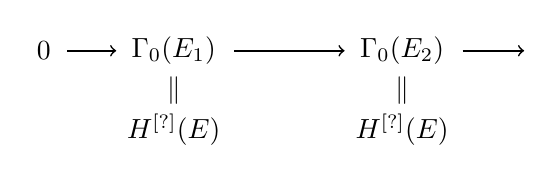
\begin{tikzpicture}[x=1cm,y=1cm]
\node at(0,0){$0$};\node at(1.65,0){$\Gamma_0(E_1)$};\node at(4.55,0){$\Gamma_0(E_2)$};
\draw[line width=.6pt,->](.30,0)--(.92,0);
\draw[line width=.6pt,->](2.42,0)--(3.82,0);
\draw[line width=.6pt,->](5.32,0)--(6.10,0);
\node at(1.65,-.50){$\Vert$};\node at(4.55,-.50){$\Vert$};
\node at(1.65,-1.00){$H^{[?]}(E)$};\node at(4.55,-1.00){$H^{[?]}(E)$};
\end{tikzpicture}\end{center}
\Unclear{GELFAND-P000104}{cohomology-overwrite}{Beneath two terms of the chain, vertical double strokes and entries $H^{[?]}(E)$. Both superscripts are densely overwritten: $H^*(E)$ / $H^i(E)$ / illegible degree. Former strokes remain inseparable even under enlargement. The chain's last arrow has no visible continuation or ellipsis.}
\end{GelfandAdjacentEvidence}
\begin{GelfandAdjacentEvidence}{GELFAND-P000104}{61}

\underline{Remark.} $\pi_\lambda$ commutes with $d$.
\SourceFigure{GELFAND-P000104}{commuting-projection-remark}{Remark. has a straight underline; then $\pi_\lambda$ commutes with d.}
\end{GelfandAdjacentEvidence}
\begin{GelfandAdjacentEvidence}{GELFAND-P000104}{62}

\begin{equation*}\left\{\begin{aligned}\sum(-1)^i\operatorname{tr}(T_0^i)&=L(T,E)\\(-1)^i\operatorname{tr}(T_\lambda^i)&=0\end{aligned}\right.\end{equation*}
\Unclear{GELFAND-P000104}{last-sum-absent}{A shared left brace. Only the first row starts with $\sum$; no separate sum is visible before $(-1)^i$ in the second row. T has superscript i in both rows; lower signs 0 and $\lambda$.}
\end{GelfandAdjacentEvidence}
\begin{GelfandAdjacentEvidence}{GELFAND-P000105}{63}



\SourcePage{GELFAND-P000105}{69}
If there is a seq. of spaces
\begin{equation*}0\longrightarrow A_1\overset{d}{\longrightarrow}A_2\overset{d}{\longrightarrow}\cdots\overset{d}{\longrightarrow}A_n\longrightarrow0,\qquad d^2=0.\end{equation*}
and maps $T_i$, comm. with $d$. Then
\begin{equation*}\underset{\text{in chains}}{\sum(-1)^i\operatorname{tr}T_i}=\underset{\text{in homol.}}{\sum(-1)^i\operatorname{tr}(T_i^*)}\qquad(\text{Euler's formula})\end{equation*}
(Euler's formula is obtained by taking $T=E$)
\SourceFigure{GELFAND-P000105}{euler-chain-annotations}{The chain's end arrows are unlabelled, its internal arrows have d. Beneath the left sum, a separate stroke and in chains; beneath the right, a stroke and in homol. At right, a parenthesis Euler's formula.}
\end{GelfandAdjacentEvidence}
\begin{GelfandAdjacentEvidence}{GELFAND-P000105}{64}


\underline{Proof}: represent.
\begin{equation*}A_i=\underset{\text{$Z$ 3 summands.}}{Z}+C_Z,\qquad Z=B+\text{compl.}\end{equation*}
and then consider $T$ there.
\SourceFigure{GELFAND-P000105}{proof-decomposition}{Proof has a straight underline; the colon is to the right of the line. Beneath the first Z, a separate entry Z 3 summands. The second entry is $Z=B+\text{compl.}$; then and then consider T there.}
\end{GelfandAdjacentEvidence}
\begin{GelfandAdjacentEvidence}{GELFAND-P000105}{65}

It suffices to replace $\operatorname{tr}T_\lambda$ by $\operatorname{tr}T_\lambda^*$,
and [crossed out: illegible entry] $H_\lambda=0$.
\Unclear{GELFAND-P000105}{homology-cancel}{Before $H_\lambda=0$, a long densely cancelled entry with loops at both ends and a horizontal stroke. Former letters remain inseparable.}
\end{GelfandAdjacentEvidence}
\begin{GelfandAdjacentEvidence}{GELFAND-P000105}{66}


Introduce
\begin{equation*}\operatorname{tr}^z(E_i)=\sum_\lambda(1+\lambda)^{-z}\operatorname{tr}(T_\lambda^*|E_i)\end{equation*}
for $\operatorname{Re}z>\frac12\dim X$,
\SourceFigure{GELFAND-P000105}{regularized-trace-definition}{The sum has subscript $\lambda$, the factor exponent $-z$, and $T_\lambda$ a superscript star. The next line is for $\operatorname{Re}z>\frac12\dim X$, followed by a comma.}
\end{GelfandAdjacentEvidence}
\begin{GelfandAdjacentEvidence}{GELFAND-P000105}{67}

[At right:]
\begin{equation*}\lambda_n\sim n^{K/\dim X}\end{equation*}
\Unclear{GELFAND-P000105}{eigenvalue-power}{The exponent's numerator is a K-like sign with a straight left stroke and two right branches: $K$ / $\kappa$.}
\end{GelfandAdjacentEvidence}
\begin{GelfandAdjacentEvidence}{GELFAND-P000105}{68}

\begin{equation*}\sum(-1)^i\operatorname{tr}^z(T_i^i)=L(T,E)\qquad\text{for all }z.\end{equation*}
\Unclear{GELFAND-P000105}{trace-argument}{In parentheses after tr, a dense T with a lower i-like sign and a separate upper i-like sign: $T_i^i$ / $T_i$ / illegible superscript.}
\end{GelfandAdjacentEvidence}
\begin{GelfandAdjacentEvidence}{GELFAND-P000105}{69}


\uwave{Continuation theorem}
(reference to Narashimhan a[?] and others.)
\Unclear{GELFAND-P000105}{continuation-name}{A Latin name with joined m/h/n-like loops and a separate final a: Narashimhan a[?] / Narasimhcan a / Narasimhana. Beneath, Nirenberg with a densely overwritten ending; then two more names.}
\end{GelfandAdjacentEvidence}
\begin{GelfandAdjacentEvidence}{GELFAND-P000105}{70}

[Above and others.: katase.[?]]
\Unclear{GELFAND-P000105}{continuation-side-name}{A separate small entry above and others.: source катаcэ. / катасэ. (katase.[?]) / illegible. The last sign resembles э; some forms also permit a Latin c.}
\end{GelfandAdjacentEvidence}
\begin{GelfandAdjacentEvidence}{GELFAND-P000105}{71}

[Beneath: Nirenberg, Cohna[?], Hörmander.]
\Unclear{GELFAND-P000105}{continuation-middle-name}{The middle Latin name between commas: Cohna / Cohn a. Between h and final a, dense joined strokes; exact separation of letters is undetermined.}
\end{GelfandAdjacentEvidence}
\begin{GelfandAdjacentEvidence}{GELFAND-P000105}{72}

\par $\operatorname{tr}^zT^i$ extends to the whole plane, is analytic throughout the plane (!) and at $z=0$

\begin{equation*}\operatorname{tr}^0(T^i)=\operatorname{tr}^{[?]}(T^i)\end{equation*}

where $\operatorname{tr}^b$ — the trace, calc. in the usual way through generalized functions.
\SourceFigure{GELFAND-P000105}{continuation-theorem-heading}{The heading Continuation theorem has a wavy underline. The text twice mentions the whole plane, with a separate (!) and at $z=0$. T has superscript i.}
\end{GelfandAdjacentEvidence}
\begin{GelfandAdjacentEvidence}{GELFAND-P000105}{73}

\Unclear{GELFAND-P000105}{trace-superscript-overwrite}{The second tr's superscript is densely overwritten and joins surrounding strokes: b[?] / illegible. Beneath and later at left, $\operatorname{tr}^b$ is clearly written.}
\end{GelfandAdjacentEvidence}
\begin{GelfandAdjacentEvidence}{GELFAND-P000105}{74}



$T=E$ does not work (giving $\zeta(s)$[?] with poles), but consider
[Insertion beneath $T=E$:] $(\operatorname{tr}E=\infty\text{ at }z=0)$.

an oper. [illegible sign], having a finite no. of fixed points (simple).
\Unclear{GELFAND-P000105}{identity-pole-insertion}{Before (s), a large zigzag sign with a rounded lower exit: $\zeta$[?] / $\Sigma$[?]. Beneath the line, a separate parenthesis $\operatorname{tr}E=\infty$ at $z=0$.}
\end{GelfandAdjacentEvidence}
\begin{GelfandAdjacentEvidence}{GELFAND-P000105}{75}


\Unclear{GELFAND-P000105}{operator-mark}{After oper., a dense vertical overwritten entry with several transverse projections and lower legs; no secure letter reading. Then a comma, having a finite no. of fixed points (simple).}
\end{GelfandAdjacentEvidence}
\begin{GelfandAdjacentEvidence}{GELFAND-P000105}{76}


$\operatorname{tr}^b$: $T$ is given as a kernel, $\int\kappa(x,x)\,dx$.
\Unclear{GELFAND-P000105}{kernel-letter-shape}{The kernel letter has a K-/к-like form: $\kappa$ / $K$. A short dense sign in the integral, a taller left stroke in the two-argument formula. The handwritten height does not establish alphabet or case.}
\end{GelfandAdjacentEvidence}
\begin{GelfandAdjacentEvidence}{GELFAND-P000105}{77}

$\operatorname{tr}^b$ — calc. through fixed points.
[Above fixed: (generalized functions).]
(A version using a seq. of functions, conv.[?] to a $\delta$-function)
Some variant of the b-trace.
\Unclear{GELFAND-P000105}{distribution-approximation-overwrite}{In the parenthesis, the word before to a $\delta$-function is densely overwritten: source сход.[?] (conv.[?]) / illegible beginning. Former strokes remain inseparable. Above the preceding fixed, a separate insertion (generalized functions).}
\end{GelfandAdjacentEvidence}
\begin{GelfandAdjacentEvidence}{GELFAND-P000105}{78}

[At right:] $\delta(x,a)$ — $\delta$ at the point $a$.
\begin{equation*}s(x)\longrightarrow\varphi s(f(x))\end{equation*}
(transf.[?] of traces) $x\longrightarrow f(x)$
\begin{equation*}\kappa(x,y)=\delta(y\,{[?]}\,f(x))\end{equation*}
\Unclear{GELFAND-P000105}{kernel-argument}{The first argument and following sign to the right of $\delta$ are densely overwritten. Readings $y-f(x)$ / $y,f(x)$ / illegible. No separate untouched minus stroke can be distinguished between the overwritten y and f.}
\end{GelfandAdjacentEvidence}
\begin{GelfandAdjacentEvidence}{GELFAND-P000105}{79}

The operator's trace $\int\kappa(x,x)\,dx$.
\begin{equation*}\int\delta(x,f(x))\,dx\end{equation*}
— the number of fixed points; if there is $\varphi$, the trace of $\varphi$ enters. Justified as usual.
\SourceFigure{GELFAND-P000105}{delta-comma-trace}{At right, $\delta(x,a)$ with a comma and an entry about the point a. The lower integral $\delta(x,f(x))$ also has a comma. At left, the map with $\varphi$; at right, a parenthesis source пробр. следов (transf.[?] of traces) and a separate $x\longrightarrow f(x)$.}
\end{GelfandAdjacentEvidence}
\begin{GelfandAdjacentEvidence}{GELFAND-P000105}{80}


\underline{Next time Kazhdan will also speak.}
\par\underline{Kazhdan} 5 minutes.
\SourceFigure{GELFAND-P000105}{kazhdan-heading}{The entire first phrase has a straight underline. Beneath, Kazhdan is separately underlined, followed by 5 minutes.}
\end{GelfandAdjacentEvidence}
\begin{GelfandAdjacentEvidence}{GELFAND-P000105}{81}

$X$ — top. space, $O$ — sheaf of rings, $M$ — sheaf of modules.
It is of finite type if $\forall x\in X$ $\exists\underset{x}{\underset{\Downarrow}{U}}$ and a fin. set of sections
$f_i\in\Gamma(U,M)$, such that $\forall y\in U$, the $f_i$ in the fibre over $y$
generate [crossed out: illegible word] the module $M_y$.
\SourceFigure{GELFAND-P000105}{module-neighborhood}{Beneath U after $\exists$, a double downward arrow to x. This x is separate from y in the next line over y. The text first has $\forall x\in X$, then $\forall y\in U$.}
\end{GelfandAdjacentEvidence}
\begin{GelfandAdjacentEvidence}{GELFAND-P000105}{82}

\Unclear{GELFAND-P000105}{module-cancel}{Between generate and module, a long densely cancelled word with a lower loop at left and a horizontal stroke to the right. Former letters remain inseparable.}
\end{GelfandAdjacentEvidence}
\begin{GelfandAdjacentEvidence}{GELFAND-P000105}{83}

\begin{gather*}f_i\in\Gamma(U,M)\qquad\exists\text{ map }O_U^n\longrightarrow M_U\qquad\text{from the set }f_i\\a_1,\ldots,a_n\longrightarrow a_1f_1+a_2f_2+\cdots+a_nf_n.\end{gather*}
$\operatorname{Ker}$ is called the sheaf of relations. Req., that $\forall$ set



\SourcePage{GELFAND-P000106}{unlabelled}
of sections the sheaf of rel. should be of finite type.
\SourceFigure{GELFAND-P000105}{module-presentation}{O has superscript n and subscript U; M has subscript U. The coefficient arrow points right; at right a linear combination through $a_nf_n$ and a period. On the last line the abbreviation source Треб. (Req.) has a separate following comma; the line ends $\forall$ set.}
\end{GelfandAdjacentEvidence}
\begin{GelfandAdjacentEvidence}{GELFAND-P000106}{84}


(Insuff. for fixed sections $f_i$, since a point, $1$, a non-Noeth. ring)
\Unclear{GELFAND-P000106}{isolated-one}{Between a point, and a non-Noeth. ring, a separate 1 with a following comma. The sign has no label; its role is undetermined.}
\end{GelfandAdjacentEvidence}
\begin{GelfandAdjacentEvidence}{GELFAND-P000106}{85}

(see Serre, “Coher. alg. sheaves”)
\par If $N\subset M$, N — a subsheaf of fin. type, then it is coherent.
(For Noeth. rings one can require less)
\SourceFigure{GELFAND-P000106}{coherence-source-and-reference}{The page begins with the continuation of sections the sheaf of rel. should be of finite type. The reference has a comma after Serre, then quotation marks. The next assertion has a separate $N\subset M$, then N — a subsheaf of fin. type.}
\end{GelfandAdjacentEvidence}
\begin{GelfandAdjacentEvidence}{GELFAND-P000106}{86}

If in an exact seq.
\begin{equation*}0\longrightarrow M'\longrightarrow M\longrightarrow M''\longrightarrow0\end{equation*}

2 [densely crossed out: illegible word; written above: sheaves[?]]
are coher., the 3rd is coher. too.
\SourceFigure{GELFAND-P000106}{exact-coherent-sequence}{The chain has M with one prime, M without primes, and M with two primes; all four arrows are unlabelled.}
\end{GelfandAdjacentEvidence}
\begin{GelfandAdjacentEvidence}{GELFAND-P000106}{87}


\Unclear{GELFAND-P000106}{two-sheaves-overwrite}{Above the densely cancelled entry, source пучка (sheaves)[?] / illegible. Beneath the addition, long horizontal strokes and lower loops; the former word remains inseparable.}
\end{GelfandAdjacentEvidence}
\begin{GelfandAdjacentEvidence}{GELFAND-P000106}{88}

$x$. The $f_i$ gen. the module at the point $x$; then they gen. the module in a \underline{neighb.} of the \underline{point} $x$.
\SourceFigure{GELFAND-P000106}{neighborhood-underlines}{An isolated x followed by a period at the beginning. In the lower line, two separate straight strokes at neighb. and point; none beneath the last x.}
\end{GelfandAdjacentEvidence}
\begin{GelfandAdjacentEvidence}{GELFAND-P000106}{89}


\underline{S. Gelfand.} Alg. def. of the $K$-functor.
$A$ — a (commut.) ring. $K_0(A)$. Consider left proj. modules over $A$ and form the free group $[P]$ on them, abelian. Quotient
by exact seq.
\begin{equation*}0\longrightarrow P_1\longrightarrow P\longrightarrow P_2\longrightarrow0\end{equation*}
by the rel. $[P]-[P_1]-[P_2]$, obtaining $K_0(A)$
\SourceFigure{GELFAND-P000106}{K0-definition}{S. Gelfand. is separately underlined. The chain has $P_1$, P, $P_2$; the next line has $[P]-[P_1]-[P_2]$, with no $=0$ written beside it, then obtaining $K_0(A)$.}
\end{GelfandAdjacentEvidence}
\begin{GelfandAdjacentEvidence}{GELFAND-P000106}{90}

$(P=P_1+P_{[?]})$.
\Unclear{GELFAND-P000106}{split-subscript}{The last lower sign in the parenthesis has two rounded parts and a dense lower curve: $2$[?] / $3$[?]. The neighbouring chain and relation have lower 2 signs with flatter ends. The final index remains undetermined.}
\end{GelfandAdjacentEvidence}
\begin{GelfandAdjacentEvidence}{GELFAND-P000106}{91}

What if one takes $E(X)$ and all modules of finite type.
\Unclear{GELFAND-P000106}{E-X-letter}{Before (X), a rounded E-like letter with three exits to the right: E / calligraphic E / an $\varepsilon$-like form. Alphabet and exact case are not established by this sign.}
\end{GelfandAdjacentEvidence}
\begin{GelfandAdjacentEvidence}{GELFAND-P000106}{92}

$P$ — in topology, a loc. triv. bundle (sheaf of rings of cont. functions)
\par A proj. mod over $A$ is loc. free in the localization at a prime ideal (all if $A$ is commut.). A proj. mod over a loc.
[crossed out: ring] is free.
\SourceFigure{GELFAND-P000106}{projective-local-cancel}{After loc., the next line has ring crossed out, then a separate is free. The parenthesis says all if A is commut.}
\end{GelfandAdjacentEvidence}
\begin{GelfandAdjacentEvidence}{GELFAND-P000106}{93}


$1/\underline{\overline{XI}}$ \underline{Smirnov.} Positive-def. functions on a group. Describe the extreme points. (cont. representations) for groups $G$ obtained from a nilp. alg. by introducing mult. by the Campbell — Hausdorff formula.
\SourceFigure{GELFAND-P000106}{smirnov-heading}{XI in the date has separate over- and underlines. Smirnov. is separately underlined. Then Positive-def. functions on a group and the entry about the Campbell — Hausdorff formula.}
\end{GelfandAdjacentEvidence}
\begin{GelfandAdjacentEvidence}{GELFAND-P000106}{94}


\underline{Gelfand.} Again on Atiyah.
$S(x)\in\Gamma(E_i)$, $\varphi(x)s(f^{-1}(x))$. This is $\int\kappa(x,y)s(y)\,dy$.
For fixed $y$, $\kappa(x,y)\in\operatorname{Hom}(E_y,E_x)$,
\SourceFigure{GELFAND-P000106}{section-case-and-inverse}{An uppercase S(x) at the beginning; lowercase s after $\varphi(x)$ and in the integral. The first f has an explicit superscript $-1$. Hom has lower signs y and x. The kernel letter has K-/к-like strokes.}
\end{GelfandAdjacentEvidence}
\begin{GelfandAdjacentEvidence}{GELFAND-P000106}{95}

[Densely crossed out: $\operatorname{tr}$[?]] $=\int\kappa(x,x)\,dx$.
\Unclear{GELFAND-P000106}{trace-cancel}{Before the equality, a dense overwritten entry: tr[?] / illegible. The upper transverse stroke and lower loops merge; former lines remain inseparable.}
\end{GelfandAdjacentEvidence}
\begin{GelfandAdjacentEvidence}{GELFAND-P000106}{96}

\begin{equation*}\kappa(x,y)=\text{[crossed out: ?]}\,\varphi(x)\delta(y-f(x)).\end{equation*}
\Unclear{GELFAND-P000106}{kernel-cancel}{Between the equality and $\varphi(x)$, a dense cancelled vertical sign with upper and lower loops. Exact reading undetermined. A minus stroke is visible in the following $\delta$ argument: $y-f(x)$.}
\end{GelfandAdjacentEvidence}
\begin{GelfandAdjacentEvidence}{GELFAND-P000106}{97}

The operator's trace $\int\operatorname{tr}(\kappa(x,x))\,dx$.
\begin{equation*}\int\operatorname{tr}(\varphi(x))\delta(x-f(x))\,dx=\sum_\rho\frac{\operatorname{tr}\varphi(\rho)}{|1-J_\rho(f)|}.\end{equation*}

(by the change-of-variables formula for the $\delta$-function)
\Unclear{GELFAND-P000106}{fixed-point-denominator}{The sign before subscript $\rho$ is curved, with a short upper exit and a hooked lower part: $J_\rho(f)$[?] / $D_\rho(f)$ / $\text{Д}_\rho(f)$. Two vertical outer bars. No separate det entry is visible in the denominator.}
\end{GelfandAdjacentEvidence}
\begin{GelfandAdjacentEvidence}{GELFAND-P000106}{98}



\underline{Lemma from lin. algebra.} $C_i$ — lin. spaces.
$d^2=0$. $T$ commutes with $d$.
\begin{center}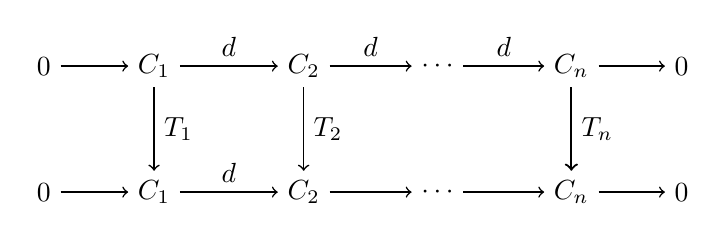
\begin{tikzpicture}[x=1cm,y=1cm]
\node(u0)at(0,0){$0$};\node(u1)at(1.4,0){$C_1$};\node(u2)at(3.3,0){$C_2$};
\node(ud)at(5,0){$\cdots$};\node(un)at(6.7,0){$C_n$};\node(uz)at(8.1,0){$0$};
\node(v0)at(0,-1.6){$0$};\node(v1)at(1.4,-1.6){$C_1$};\node(v2)at(3.3,-1.6){$C_2$};
\node(vd)at(5,-1.6){$\cdots$};\node(vn)at(6.7,-1.6){$C_n$};\node(vz)at(8.1,-1.6){$0$};
\draw[->,line width=.55pt](u0)--(u1);
\draw[->,line width=.55pt](u1)--node[above]{$d$}(u2);
\draw[->,line width=.55pt](u2)--node[above]{$d$}(ud);
\draw[->,line width=.55pt](ud)--node[above]{$d$}(un);
\draw[->,line width=.55pt](un)--(uz);
\draw[->,line width=.55pt](v0)--(v1);
\draw[->,line width=.55pt](v1)--node[above]{$d$}(v2);
\draw[->,line width=.55pt](v2)--(vd);
\draw[->,line width=.55pt](vd)--(vn);
\draw[->,line width=.55pt](vn)--(vz);
\draw[->,line width=.6pt](u1)--node[right]{$T_1$}(v1);
\draw[->,line width=.6pt](u2)--node[right]{$T_2$}(v2);
\draw[->,line width=.8pt](un)--node[right]{$T_n$}(vn);
\end{tikzpicture}\end{center}
\SourceFigure{GELFAND-P000106}{linear-algebra-diagram}{Two horizontal chains, with 0 at their ends. The upper row has three internal d labels; the lower row has d only between $C_1$ and $C_2$. Three downward vertical marks labelled $T_1$, $T_2$, $T_n$. The right mark has a dense diamond-like lower end; beneath it the lower $C_n$ is densely overwritten. The typographic recreation preserves direction and labels; dense contours remain inseparable.}
\end{GelfandAdjacentEvidence}
\begin{GelfandAdjacentEvidence}{GELFAND-P000106}{99}

\begin{equation*}\frac{\operatorname{Ker}d|C_i}{\operatorname{Im}C_{i-1}}=H^i.\end{equation*}
\SourceFigure{GELFAND-P000106}{cohomology-quotient}{The manuscript fraction bar is oblique. Above it, Ker $d|C_i$; beneath, a dense Im $C_{i-1}$, with no separate d or restriction bar visible after Im. At right, $=H^i$.}
\end{GelfandAdjacentEvidence}
\begin{GelfandAdjacentEvidence}{GELFAND-P000106}{100}

$T_i^*:H^i\longrightarrow H^i$.
\begin{equation*}\sum(-1)^i\operatorname{tr}T_i=\sum(-1)^i\operatorname{tr}(T_i^*).\end{equation*}
\SourceFigure{GELFAND-P000106}{final-traces}{At left, $T_i^*:H^i\longrightarrow H^i$. In the last equality both sums have superscript i on $(-1)$; tr $T_i$ at left, tr($T_i^*$) at right.}
\end{GelfandAdjacentEvidence}
\begin{GelfandAdjacentEvidence}{GELFAND-P000107}{101}



\SourcePage{GELFAND-P000107}{70}
[Crossed out at the top: This[?] $C^\infty$ that[?]; the rest illegible.]
\Unclear{GELFAND-P000107}{top-cancel}{A long stroke crosses the top line; dense writing beneath it on the left, $C^\infty$ in the middle, that[?] on the right. The word boundaries and exact reading are not established.}
\end{GelfandAdjacentEvidence}
\begin{GelfandAdjacentEvidence}{GELFAND-P000107}{102}

This is a finite analogue.
\par\underline{Applications.}
\par 1. Usual Lefschetz formula.
$X\overset{f}{\longrightarrow}X$ isol. sing. points.
De Rham complex.
[On the right:]
\begin{gather*}
\bigl(\sum\text{ mult. of fixed points}\,=\\
=\sum\text{ traces on cohom.}
\end{gather*}
\SourceFigure{GELFAND-P000107}{opening-applications}{This is a finite analogue. is separate from the crossed line. Applications. is underlined. On the right an opening parenthesis precedes the sum; an equals sign ends the upper line and another begins the lower one. No closing parenthesis is visible.}
\end{GelfandAdjacentEvidence}
\begin{GelfandAdjacentEvidence}{GELFAND-P000107}{103}

\begin{equation*}
\underline{\operatorname{tr}\varphi_i(\rho)=\operatorname{det}-1}\,;
\end{equation*}
(computed by eigenvalues)
\Unclear{GELFAND-P000107}{de-rham-determinant}{After det a horizontal minus and a 1-like sign; the readings $-1$ / $-I$ and an illegible argument remain undistinguished. A long line below the entire expression turns upward at the right.}
\end{GelfandAdjacentEvidence}
\begin{GelfandAdjacentEvidence}{GELFAND-P000107}{104}

[On the right:]
\begin{equation*}\sum\pm1\quad\text{over fixed points}.\end{equation*}
\begin{equation*}
\sum(\pm1)\lambda_{i_1}\cdots\lambda_{i_k}\qquad
J_\rho=\begin{pmatrix}\lambda_1&&0\\&\ddots&\\0&&\lambda_n\end{pmatrix}
\end{equation*}
[A diagonal ellipsis lies between $\lambda_1$ and $\lambda_n$ in the matrix.]
\SourceFigure{GELFAND-P000107}{exterior-trace-matrix}{The sum has a separate $(\pm1)$, then $\lambda_{i_1}\cdots\lambda_{i_k}$. On the right a J-like letter with subscript $\rho$; inside parentheses $\lambda_1$ at upper left, $\lambda_n$ at lower right, zeros at the other corners and a diagonal ellipsis between them.}
\end{GelfandAdjacentEvidence}
\begin{GelfandAdjacentEvidence}{GELFAND-P000107}{105}

\par 2. Complex case.
$f:X\longrightarrow X$ — holom.
\begin{equation*}\sum f_{i_1\cdots i_k}\,dz_{i_1}\wedge\cdots\wedge dz_{i_k}\end{equation*}
$f_{i_1\cdots i_k}$ holom. and holom. diff. $H^{i,0}($
\begin{flushright}\begin{tikzpicture}[x=1cm,y=1cm]
\draw[line width=.55pt](0,1.8)--(0,-.15);
\draw[line width=.55pt](0,0)--(1.4,0);
\end{tikzpicture}\end{flushright}
\SourceFigure{GELFAND-P000107}{complex-forms-corner}{To the right of the lines of forms a long vertical stroke downward and a horizontal stroke to the right from it; the corner has no arrows or labels. The parenthesis at $H^{i,0}($ remains open.}
\end{GelfandAdjacentEvidence}
\begin{GelfandAdjacentEvidence}{GELFAND-P000107}{106}

[Densely crossed out below $H^{i,0}($: illegible.]
\Unclear{GELFAND-P000107}{holomorphic-cancel}{Below the open parenthesis dense horizontal strokes slope upward to the right; individual letters are not distinguished.}
\end{GelfandAdjacentEvidence}
\begin{GelfandAdjacentEvidence}{GELFAND-P000107}{107}

\begin{equation*}
\sum(-1)^i\frac{\operatorname{tr}\varphi(E_i)}{|(1-J(f))|^2}=
\end{equation*}
[Crossed out: $\sum_\rho\operatorname{Re}($; followed by:]
\begin{equation*}\sum_\rho\operatorname{Re}\left(\frac{2}{1-J_f}\right)\end{equation*}
\Unclear{GELFAND-P000107}{complex-denominator}{The vertical strokes at the denominator are thickened: absolute value / double bars. Inside, a J-like letter / handwritten Cyrillic D; the numerator of the active sum on the right is 2, with two close horizontal lines below it.}
\end{GelfandAdjacentEvidence}
\begin{GelfandAdjacentEvidence}{GELFAND-P000107}{108}

\begin{center}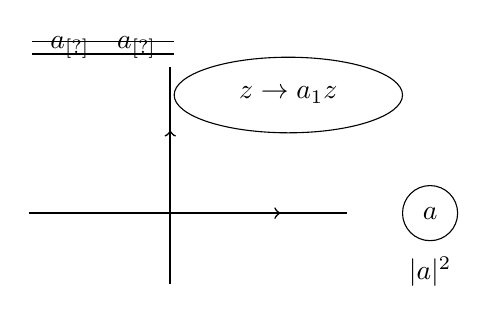
\begin{tikzpicture}[x=1cm,y=1cm]
\draw[line width=.6pt](-1.8,0)--(2.25,0);
\draw[->,line width=.6pt](0,0)--(1.4,0);
\draw[line width=.6pt](0,-.9)--(0,1.85);
\draw[->,line width=.6pt](0,0)--(0,1.05);
\node at(1.5,1.5){$z\to a_1z$};
\draw(1.5,1.5)ellipse(1.45cm and .48cm);
\node at(3.3,0){$a$};\draw(3.3,0)circle(.35cm);
\node at(3.3,-.75){$|a|^2$};
\node at(-.85,2.1){$a_{[?]}\quad a_{[?]}$};
\draw[line width=.7pt](-1.75,2.18)--(.05,2.18);
\draw[line width=.7pt](-1.75,2.02)--(.05,2.02);
\end{tikzpicture}\end{center}
\Unclear{GELFAND-P000107}{complex-axes}{Two intersecting lines, arrows upward and to the right; the horizontal line continues beyond the arrowhead. In an oval $z\to a_1z$, separately a circled a, below it $|a|^2$. Above the vertical line crossed a-like signs with illegible lower strokes; the exact reading of this writing is not established.}
\end{GelfandAdjacentEvidence}
\begin{GelfandAdjacentEvidence}{GELFAND-P000107}{109}

When the transf. $\Vert$ is fractional-linear, this is the fixed-point theorem.
\SourceFigure{GELFAND-P000107}{mobius-statement}{Two vertical lines stand between transf. and fractional-linear. The final words fixed point. are on the next line.}
\end{GelfandAdjacentEvidence}
\begin{GelfandAdjacentEvidence}{GELFAND-P000107}{110}

\begin{equation*}
=\frac{1}{[?]}\left(\frac{1}{\overline{1-J(f)}}+\frac{1}{1-J(f)}\right)
\end{equation*}
\Unclear{GELFAND-P000107}{conjugate-average}{Below the first separate 1 a dense sign: 2[?] / 1[?] / illegible. The first inner fraction has two long horizontal lines, the second one; the first extra line may indicate conjugation of the fraction or denominator.}
\end{GelfandAdjacentEvidence}
\begin{GelfandAdjacentEvidence}{GELFAND-P000107}{111}

The real trace, is [crossed out: illegible] the sum of the complex and complex-conjugate traces.
\Unclear{GELFAND-P000107}{real-trace-cancel}{Between is and the sum a densely crossed horizontal record with a vertical stroke at the right; individual letters are not distinguished.}
\end{GelfandAdjacentEvidence}
\begin{GelfandAdjacentEvidence}{GELFAND-P000107}{112}

Appl. also to [heavily overwritten: illegible] fractional-linear transf. of projective \underline{space}.
\Unclear{GELFAND-P000107}{projective-cancel}{After also to two dense superposed signs. Under the abbreviation for space two separate short lines; the preceding overwritten writing is illegible.}
\end{GelfandAdjacentEvidence}
\begin{GelfandAdjacentEvidence}{GELFAND-P000107}{113}

\par\underline{Kazhdan.} \underline{Definition} \underline{of homology} \underline{of anything.}
\SourceFigure{GELFAND-P000107}{kazhdan-heading}{The surname and three parts of the heading have separate underlines. The Russian words for of anything are joined by a hyphen.}
\end{GelfandAdjacentEvidence}
\begin{GelfandAdjacentEvidence}{GELFAND-P000107}{114}

$C$ — an abelian category. an object $Q$ is called injective if the functor $F(A)=\operatorname{Hom}(A,Q)$ is exact.
($A'\subset A$ $\forall f$ [crossed out: an illegible word] extends)
\begin{center}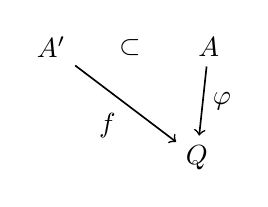
\begin{tikzpicture}[x=1cm,y=1cm]
\node(ap)at(0,0){$A'$};\node at(1,0){$\subset$};\node(a)at(2,0){$A$};
\node(q)at(1.85,-1.4){$Q$};
\draw[->,line width=.6pt](ap)--node[below left]{$f$}(q);
\draw[->,line width=.6pt](a)--node[right]{$\varphi$}(q);
\end{tikzpicture}\end{center}
\SourceFigure{GELFAND-P000107}{injective-definition-diagram}{Within the parentheses $A'\subset A$; from $A'$ an arrow downward to the right labelled f, from A downward to Q an arrow with $\varphi$ at the right. There is no superscript at $F(A)$.}
\end{GelfandAdjacentEvidence}
\begin{GelfandAdjacentEvidence}{GELFAND-P000107}{115}

\Unclear{GELFAND-P000107}{extension-cancel}{After $\forall f$ above extends a densely crossed word; its letters are not separated.}
\end{GelfandAdjacentEvidence}
\begin{GelfandAdjacentEvidence}{GELFAND-P000107}{116}

The categ. has enough injective objects if $\forall A$ $\exists$ inj. $Q$ $\Vert$ $0\longrightarrow A\longrightarrow Q$.
[cat. of sheaves]
\SourceFigure{GELFAND-P000107}{enough-injectives}{Before $0\to A\to Q$ two vertical lines, with the lower part thickened. On the right a separate record in square brackets cat. of sheaves.}
\end{GelfandAdjacentEvidence}
\begin{GelfandAdjacentEvidence}{GELFAND-P000107}{117}

Let there be [crossed out: illegible] a functor $F(A)$ $C\overset{F}{\longrightarrow}C'$ covar. and left exact, i.e.

\begin{equation*}
0\longrightarrow A\longrightarrow B\longrightarrow\underbrace{C\longrightarrow0}_{\text{may also be left out.}}
\Longrightarrow0\longrightarrow F(A)\longrightarrow F(B)\longrightarrow F(C)
\end{equation*}
\Unclear{GELFAND-P000107}{functor-cancel}{Between there be and a functor a small densely crossed record, with a downward projecting stroke; the exact reading is not established.}
\end{GelfandAdjacentEvidence}
\begin{GelfandAdjacentEvidence}{GELFAND-P000107}{118}


\SourceFigure{GELFAND-P000107}{functor-left-exact}{F above the arrow at $C\to C'$. Beneath $C\to0$ in the original sequence an arc with may also be left out. In the sequence after the large arrow the last visible term is $F(C)$, followed by no dot or zero.}
\end{GelfandAdjacentEvidence}
\begin{GelfandAdjacentEvidence}{GELFAND-P000107}{119}

and $C$ has enough inj. obj.
Derived functors (they $\exists$ and are unique) — functors from cat. $C$ to $C'$, satisfying the conditions:
\par 1) $F^0(A)=F(A)$
\par 2) $F^{[?]}(Q)=0$ $(i>0)$ $\forall$ injective $Q$
\Unclear{GELFAND-P000107}{derived-conditions}{In condition 1 the superscript is 0. In condition 2 the superscript above F is filled in, with a small upward projection: i[?] / 0[?] / illegible; separately $(i>0)$ at the right.}
\end{GelfandAdjacentEvidence}
\begin{GelfandAdjacentEvidence}{GELFAND-P000107}{120}

\par 3) $\forall$ exact seq. $0\longrightarrow A\longrightarrow B\longrightarrow C\longrightarrow0$ there is an exact seq.
\begin{equation*}
0\longrightarrow F^0(A)\longrightarrow F^0(B)\longrightarrow F^0(C)
\overset{\delta}{\longrightarrow}F^1(A)\longrightarrow F^1(B)\overset{\delta}{\longrightarrow}{}
\end{equation*}
\SourceFigure{GELFAND-P000107}{derived-long-sequence}{At the bottom the sequence begins 0, then three terms with superscript 0, then an arrow with $\delta$, two terms with superscript 1 and another arrow with $\delta$.}
\end{GelfandAdjacentEvidence}
\begin{GelfandAdjacentEvidence}{GELFAND-P000107}{121}

\Incomplete{GELFAND-P000107}{derived-edge}{The last arrow is at the right edge; the following term is not visible in this frame.}
\end{GelfandAdjacentEvidence}
\begin{GelfandAdjacentEvidence}{GELFAND-P000107}{122}

[Above the final arrows: induced[?] with a stroke continuing to the right.]
\Unclear{GELFAND-P000107}{induced-annotation}{The readings are induc.[?] / induc...[?]; the ending merges into a long rightward stroke ending beside the last $\delta$. The precise attachment of the stroke is not established.}
\end{GelfandAdjacentEvidence}
\begin{GelfandAdjacentEvidence}{GELFAND-P000108}{123}


\usetikzlibrary{decorations.pathmorphing}

\SourcePage{GELFAND-P000108}{unlabelled}
Moreover 3') Let there be another exact seq. and a map.
\begin{center}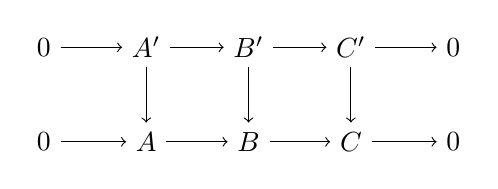
\begin{tikzpicture}[x=1cm,y=1cm]
\node(a0)at(0,0){$0$};\node(a1)at(1.3,0){$A'$};\node(a2)at(2.6,0){$B'$};\node(a3)at(3.9,0){$C'$};\node(a4)at(5.2,0){$0$};
\node(b0)at(0,-1.2){$0$};\node(b1)at(1.3,-1.2){$A$};\node(b2)at(2.6,-1.2){$B$};\node(b3)at(3.9,-1.2){$C$};\node(b4)at(5.2,-1.2){$0$};
\draw[->](a0)--(a1);\draw[->](a1)--(a2);\draw[->](a2)--(a3);\draw[->](a3)--(a4);
\draw[->](b0)--(b1);\draw[->](b1)--(b2);\draw[->](b2)--(b3);\draw[->](b3)--(b4);
\draw[->](a1)--(b1);\draw[->](a2)--(b2);\draw[->](a3)--(b3);
\end{tikzpicture}\end{center}
\SourceFigure{GELFAND-P000108}{exact-sequence-diagram}{Two rows $0\to A'\to B'\to C'\to0$ and $0\to A\to B\to C\to0$; three vertical arrows downward from the primed letters. The arrows have no labels.}
\end{GelfandAdjacentEvidence}
\begin{GelfandAdjacentEvidence}{GELFAND-P000108}{124}

\begin{center}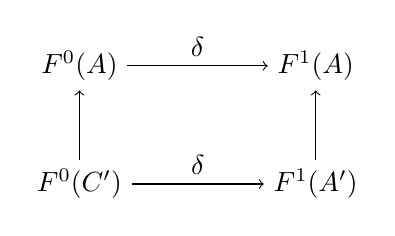
\begin{tikzpicture}[x=1cm,y=1cm]
\node(a)at(0,0){$F^0(A)$};\node(b)at(3,0){$F^1(A)$};
\node(c)at(0,-1.5){$F^0(C')$};\node(d)at(3,-1.5){$F^1(A')$};
\draw[->](a)--node[above]{$\delta$}(b);\draw[->](c)--node[above]{$\delta$}(d);
\draw[->](c)--(a);\draw[->](d)--(b);
\end{tikzpicture}\end{center}
\Unclear{GELFAND-P000108}{connecting-square-label}{At upper left $F^0(A)$: the two slanting sides and crossbar of A are visible. At upper right $F^1(A)$, below $F^0(C')$ and $F^1(A')$; both vertical arrows point upward.}
\end{GelfandAdjacentEvidence}
\begin{GelfandAdjacentEvidence}{GELFAND-P000108}{125}

\underline{Theorem}: If $A$ has enough inj. obj., the derived functors exist and are unique.
\SourceFigure{GELFAND-P000108}{theorem}{A separate large A in the hypothesis. Theorem is underlined, with the colon to the right of the line. Exist and are unique continues the writing on the next line.}
\end{GelfandAdjacentEvidence}
\begin{GelfandAdjacentEvidence}{GELFAND-P000108}{126}

\par $15/\underline{\overline{\mathrm{XI}}}$ \underline{Matsaev} \tikz[baseline=(title.base)]{\node[inner sep=0pt](title){Complete proof of the Atiyah-Bott theorem.};\draw[decorate,decoration={snake,amplitude=.45pt,segment length=5pt}] ([yshift=-2pt]title.south west)--([yshift=-2pt]title.south east);}
\SourceFigure{GELFAND-P000108}{matsaev-heading}{XI has lines above and below. A straight underline below the surname; a wavy underline below Complete proof of the Atiyah-Bott theorem.}
\end{GelfandAdjacentEvidence}
\begin{GelfandAdjacentEvidence}{GELFAND-P000108}{127}

\begin{equation*}\cdots\longrightarrow\Gamma(E_i)\overset{d}{\longrightarrow}\Gamma(E_{i+1})\longrightarrow\cdots\end{equation*}
Given $T$, acting on $\Gamma$ and commuting with $d$, $T_i^*$,
\SourceFigure{GELFAND-P000108}{bundle-complex}{d above the middle arrow of the complex, subscript $i+1$ on the right. On the next line $T_i^*$, followed by a comma.}
\end{GelfandAdjacentEvidence}
\begin{GelfandAdjacentEvidence}{GELFAND-P000108}{128}

[Densely crossed out: an illegible sign; to the right a T-like sign[?].]
\Unclear{GELFAND-P000108}{operator-cancel}{Dense crossed writing slopes upward to the right; farther right a separate small sign with a horizontal top and slanting stem: T[?] / illegible.}
\end{GelfandAdjacentEvidence}
\begin{GelfandAdjacentEvidence}{GELFAND-P000108}{129}

\begin{equation*}L(T,E)=\sum(-1)^i\operatorname{tr}T_i^*\end{equation*}
[On the right:] (Here we do not need $z$ — does not depend)
\SourceFigure{GELFAND-P000108}{L-and-parameter}{T in the sum has a superscript star and subscript i. In the right parenthesis z, then we do not need, below — does not depend.}
\end{GelfandAdjacentEvidence}
\begin{GelfandAdjacentEvidence}{GELFAND-P000108}{130}

\begin{equation*}\sum_i\sigma(\rho)\qquad\sigma(\rho)=\sum\frac{(-1)^i\operatorname{Sp}\varphi_i(\rho)}{|\operatorname{det}(1-I_f(\rho))|}\end{equation*}
\Unclear{GELFAND-P000108}{fixed-point-index}{Beneath the first sum a small sign with a separate dot above: i[?] / illegible index. In the denominator an I-like letter with a wide base / a J-like letter; followed by subscript f and $(\rho)$.}
\end{GelfandAdjacentEvidence}
\begin{GelfandAdjacentEvidence}{GELFAND-P000108}{131}

The formal proof is trivial, since
\begin{equation*}L=\sum_i(-1)^i\operatorname{tr}T_i\end{equation*}
(elem. theorem of lin. algebra)
$\operatorname{tr}T_i$ formally give this sum.
$T_i$ is given by the kernel $\varphi\delta(y-f(x))$. The trace is precisely $\sum$ over fixed points.
\SourceFigure{GELFAND-P000108}{formal-trace-kernel}{In the formal sum T has subscript i without a star. In the kernel a horizontal minus follows y, then $f(x)$. Fixed points. is carried to the next line.}
\end{GelfandAdjacentEvidence}
\begin{GelfandAdjacentEvidence}{GELFAND-P000108}{132}

Smooth by the kernel
\begin{equation*}(1+\Box)^{-z}T_i=T_{i,z},\qquad\Box=d\delta+\delta d\end{equation*}
(assume a Riem. metric is given, Herm. adjoint oper.)
[Crossed out: $(1+\Box)^{-z}$.]
The trace already exists in the usual sense.
\SourceFigure{GELFAND-P000108}{smoothing-metric}{Exponent $-z$; a comma in the right-hand $T_{i,z}$. A separate formula with a square, d and $\delta$. Below, a crossed copy of $(1+\Box)^{-z}$.}
\end{GelfandAdjacentEvidence}
\begin{GelfandAdjacentEvidence}{GELFAND-P000108}{133}

\begin{equation*}\operatorname{tr}T_{iz}=\sum_\lambda\pi_\lambda T i_\lambda(1+\lambda)^{-z}\end{equation*}
\Unclear{GELFAND-P000108}{trace-series-overwrite}{The indices of the left-hand T are densely overwritten: iz / i,z. On the right $\pi_\lambda$, T, $i_\lambda$ and $(1+\lambda)^{-z}$; no separate tr is visible after the sum.}
\end{GelfandAdjacentEvidence}
\begin{GelfandAdjacentEvidence}{GELFAND-P000108}{134}

$\sum_i(-1)^i\operatorname{tr}T_{iz}$ continues to the whole plane and at $z=0$ is an integral as a number.
\SourceFigure{GELFAND-P000108}{analytic-continuation}{Subscript i in the sum; after the whole plane and, the continuation at $z=0$ is an integral as a number.}
\end{GelfandAdjacentEvidence}
\begin{GelfandAdjacentEvidence}{GELFAND-P000108}{135}

\begin{equation*}T_{iz}=\underbrace{(1+\Box)^{-z}}_{\text{it is given by an integral kernel for sufficiently large }\operatorname{Re}z}\,T_i\end{equation*}
\SourceFigure{GELFAND-P000108}{integral-kernel-annotation}{Beneath $(1+\Box)^{-z}$ a straight bracket with a short downward stroke; the explanation below it ends in $\operatorname{Re}z$.}
\end{GelfandAdjacentEvidence}
\begin{GelfandAdjacentEvidence}{GELFAND-P000108}{136}

and this kernel is arranged as follows: [crossed out: an illegible word]
\Unclear{GELFAND-P000108}{kernel-cancel}{After arranged as follows: two dense, almost horizontal crossing strokes; the original letters are not separated.}
\end{GelfandAdjacentEvidence}
\begin{GelfandAdjacentEvidence}{GELFAND-P000108}{137}

\begin{center}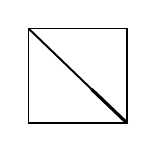
\begin{tikzpicture}[x=1cm,y=1cm]
\draw[line width=.6pt](0,0)--(0,1.2)--(1.25,1.2)--(1.25,0)--cycle;
\draw[line width=.7pt](0,1.2)--(.8,.43);
\draw[line width=1.15pt](.8,.43)--(1.25,0);
\end{tikzpicture}\end{center}
\Unclear{GELFAND-P000108}{diagonal-kernel}{An unlabelled square; the diagonal goes from upper left to lower right, thickening at the latter corner. Thickening / arrowhead[?]; it has no separate label.}
\end{GelfandAdjacentEvidence}
\begin{GelfandAdjacentEvidence}{GELFAND-P000108}{138}

off the diag. the kernel is $C^\infty$, and on the diag. breaks in the derivative (contr.[?] to Katz and Narasimhan)
\Unclear{GELFAND-P000108}{kernel-description-names}{In parentheses the abbreviation contr.[?] with a dense ending, then to Katz and Narasimhan. Before the parenthesis derivative.}
\end{GelfandAdjacentEvidence}
\begin{GelfandAdjacentEvidence}{GELFAND-P000108}{139}

The discussion concerns $(1+\Box)^{-z}$ (without $T_i$).
\SourceFigure{GELFAND-P000108}{kernel-family}{The final parenthesis reads without $T_i$. A separate $(1+\Box)^{-z}$ precedes it.}
\end{GelfandAdjacentEvidence}
\begin{GelfandAdjacentEvidence}{GELFAND-P000108}{140}

\begin{equation*}\mu_1(x)(1+\Box)^{-z}\mu_2(x)\end{equation*}
is already given by a $C^\infty$ kernel if $\operatorname{supp}[?]\,\mu_1\,\mu_2$ at the edges.
\Unclear{GELFAND-P000108}{kernel-localization}{The outer letters $\mu_1,\mu_2$ / $M_1,M_2$; the first sign is more angular. After if, supp[?] / diff.[?] / illegible; below, at the edges. The precise separator between the two letters after the abbreviation is not distinguished.}
\end{GelfandAdjacentEvidence}
\begin{GelfandAdjacentEvidence}{GELFAND-P000109}{141}



\SourcePage{GELFAND-P000109}{71}
\begin{center}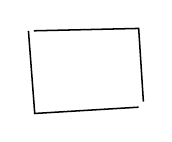
\begin{tikzpicture}[x=1cm,y=1cm]
\draw[line width=.55pt](0,1.05)--(.08,0)--(1.40,.08);
\draw[line width=.55pt](.07,1.05)--(1.40,1.08)--(1.46,.15);
\end{tikzpicture}\end{center}
\SourceFigure{GELFAND-P000109}{empty-square}{An empty quadrilateral in the upper-left margin; no diagonal or labels. The side ends do not join at lower right; a small gap also at upper left.}
\end{GelfandAdjacentEvidence}
\begin{GelfandAdjacentEvidence}{GELFAND-P000109}{142}

When can one correctly multiply two generalized fn.s with singularities on two transversal manifolds.
\SourceFigure{GELFAND-P000109}{opening-question}{The writing starts When and ends manifolds. There is no question mark at the end.}
\end{GelfandAdjacentEvidence}
\begin{GelfandAdjacentEvidence}{GELFAND-P000109}{143}

$\mu_1,\mu_2$ [crossed out: illegible]

$\cap$ supp. off the curve[?], then [crossed out: illegible]

the fn. is given by a fn.
\Unclear{GELFAND-P000109}{support-first-cancel}{Between $\mu_1,\mu_2$ and $\cap$ a short densely crossed record. The first $\mu$ has an angular top and a long lower stroke.}
\end{GelfandAdjacentEvidence}
\begin{GelfandAdjacentEvidence}{GELFAND-P000109}{144}

\Unclear{GELFAND-P000109}{support-second-cancel}{After then and before fn., dense crossed writing; the original signs are not separated.}
\end{GelfandAdjacentEvidence}
\begin{GelfandAdjacentEvidence}{GELFAND-P000109}{145}

\Unclear{GELFAND-P000109}{support-condition-word}{Off the curve[?] / off the straight line: the initial letter of the final word is dense, the next has a long lower stroke.}
\end{GelfandAdjacentEvidence}
\begin{GelfandAdjacentEvidence}{GELFAND-P000109}{146}



\usetikzlibrary{decorations.pathmorphing}
\tikz[baseline=(title.base)]{\node[inner sep=0pt](title){Suff. condition};\draw[decorate,decoration={snake,amplitude=.45pt,segment length=5pt}]([yshift=-2pt]title.south west)--([yshift=-2pt]title.south east);}: each of them is a smooth $\delta$-fn., and to it is applied an operator $P\delta_S$, if $P$ is pseudodiff. (for example, simply diff.)
\SourceFigure{GELFAND-P000109}{delta-sufficient}{A wavy underline below Suff. condition. After operator, a separate $P\delta_S$; then if $P$ is pseudodiff. The parenthesis ends simply diff.)}
\end{GelfandAdjacentEvidence}
\begin{GelfandAdjacentEvidence}{GELFAND-P000109}{147}

To it one can apply [densely crossed out: an illegible sign]

a pseudodiff. operator.
\Unclear{GELFAND-P000109}{pseudo-cancel}{Between apply and pseudodiff., a short dense sign with a lower slanting stroke.}
\end{GelfandAdjacentEvidence}
\begin{GelfandAdjacentEvidence}{GELFAND-P000109}{148}


A smooth fn. on a manifold — $\int$ over the manifold.
This is a cont. oper. on $C^\infty$ fn.s and therefore on generalized fn.s.
One must approximate the $\delta$-fn.s by $C^\infty$ fn.s in a special way, then the product will have a limit.
\SourceFigure{GELFAND-P000109}{distribution-action}{After the dash a separate integral sign without limits. Then two sentences on the cont. oper. and approximation of $\delta$-fn.s; ending in limit.}
\end{GelfandAdjacentEvidence}
\begin{GelfandAdjacentEvidence}{GELFAND-P000109}{149}

\begin{equation*}\delta(x_1)\cdot\delta(x_2)=\delta(x_1,x_2)\end{equation*}
\SourceFigure{GELFAND-P000109}{delta-product}{A dot between the first two factors; on the right $\delta(x_1,x_2)$ without a separate final period.}
\end{GelfandAdjacentEvidence}
\begin{GelfandAdjacentEvidence}{GELFAND-P000109}{150}

\begin{center}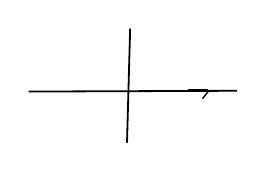
\begin{tikzpicture}[x=1cm,y=1cm]
\draw[line width=.65pt](-1.25,0)--(1.40,.01);
\draw[line width=.65pt](0,-.65)--(.04,.80);
\draw[line width=1.05pt](.78,.015)--(1.03,.015);
\draw[line width=.5pt](1.03,0)--(.96,-.09);
\end{tikzpicture}\end{center}
\Unclear{GELFAND-P000109}{transverse-lines}{Intersecting vertical and horizontal lines without labels. To the right of the intersection a short thickening and slanted stroke: arrowhead[?] / unevenness of the line. No separately marked point.}
\end{GelfandAdjacentEvidence}
\begin{GelfandAdjacentEvidence}{GELFAND-P000109}{151}

(supp. in 4-dim. space transvers. intersect. of diag.)
\SourceFigure{GELFAND-P000109}{diagonal-aside}{The parenthesis below the formula: supp. in 4-dim. space transvers. intersect. of diag.}
\end{GelfandAdjacentEvidence}
\begin{GelfandAdjacentEvidence}{GELFAND-P000109}{152}


\underline{Kazhdan.} $X_P$ — an open set in the Zariski top. $P\ne0$.
\SourceFigure{GELFAND-P000109}{kazhdan-heading-open}{The surname Kazhdan. is underlined. Then $X_P$, on the right $P\ne0$.}
\end{GelfandAdjacentEvidence}
\begin{GelfandAdjacentEvidence}{GELFAND-P000109}{153}

[On the left, crossed out: an illegible word.]
\Unclear{GELFAND-P000109}{kazhdan-cancel}{Below the underlined surname and to the left of This is a basis, several dense crossing strokes.}
\end{GelfandAdjacentEvidence}
\begin{GelfandAdjacentEvidence}{GELFAND-P000109}{154}

This is a basis of open sets on an aff. alg. variety.
Sect. of the sheaf on $X_P$: $R(x)$: $\dfrac{Q(x)}{P^n}$,

[A short sign crossed out: $=$[?] / illegible.]

they are identified if the diff. becomes 0 on the variety.
\SourceFigure{GELFAND-P000109}{sections-quotient}{Colons after $X_P$ and after $R(x)$. Numerator $Q(x)$, denominator $P^n$; a comma on the right.}
\end{GelfandAdjacentEvidence}
\begin{GelfandAdjacentEvidence}{GELFAND-P000109}{155}

\Unclear{GELFAND-P000109}{quotient-cancel}{Before they, a short dark sign with two almost horizontal strokes; original sign $=$[?].}
\end{GelfandAdjacentEvidence}
\begin{GelfandAdjacentEvidence}{GELFAND-P000109}{156}


$\Gamma(X_P,O_X)$. Aff. alg. variety — a finite number of eq.s.
$X_P$ is again an aff. space.
\SourceFigure{GELFAND-P000109}{affine-descriptions}{A period after $\Gamma(X_P,O_X)$. The final line reads precisely again an aff. space.}
\end{GelfandAdjacentEvidence}
\begin{GelfandAdjacentEvidence}{GELFAND-P000109}{157}


An algebraic sheaf — a sheaf of modules over this sheaf of rings.
Of finite type — loc. isom. to a quotient of a direct sum.
\SourceFigure{GELFAND-P000109}{algebraic-finite-type}{Two lines: the definition of an algebraic sheaf and Of finite type — loc. isom. to a quotient of a direct sum.}
\end{GelfandAdjacentEvidence}
\begin{GelfandAdjacentEvidence}{GELFAND-P000109}{158}

A coher. sheaf — further $\forall$ [crossed out: illegible] open set and $\forall$ finite coll. of sections, the sheaf of rel.s is of finite type.
\Unclear{GELFAND-P000109}{coherent-cancel}{After the first $\forall$ a densely crossed word. Then open set and $\forall$ finite coll.; continuation on the next line of sections, the sheaf of rel.s is of finite type.}
\end{GelfandAdjacentEvidence}
\begin{GelfandAdjacentEvidence}{GELFAND-P000109}{159}

\underline{Theorem}: the sheaf $O$ itself is coherent.
\SourceFigure{GELFAND-P000109}{structure-coherent-theorem}{Theorem is underlined, with the colon to the right. After the sheaf a separate O, then itself is coherent.}
\end{GelfandAdjacentEvidence}
\begin{GelfandAdjacentEvidence}{GELFAND-P000109}{160}


First for the whole aff. [crossed out: variety[?] / illegible.] [Inserted above: space.] From this everything follows autom.
\Unclear{GELFAND-P000109}{variety-cancel}{Beneath the insertion space, a crossed record variety[?]. After it a period; From this everything follows continues on the same line, autom. below.}
\end{GelfandAdjacentEvidence}
\begin{GelfandAdjacentEvidence}{GELFAND-P000109}{161}

$X_P$ — an open set. Consider a finite collection of sections
\begin{equation*}\left(\frac{Q_1}{P^n},\frac{Q_2}{P^n},\ldots,\frac{Q_i}{P^n}\right)\end{equation*}
Sheaf of relations:
\SourceFigure{GELFAND-P000109}{localized-sections}{The tuple has subscripts $1,2,\ldots,i$, denominators $P^n$; no separate period after the parenthesis. On the right Sheaf of relations:}
\end{GelfandAdjacentEvidence}
\begin{GelfandAdjacentEvidence}{GELFAND-P000109}{162}

Ring $A=k[x_1,\ldots,x_n]$. [On the right again: Sheaf of relations]
\SourceFigure{GELFAND-P000109}{relations-ring}{Ring $A=k[x_1,\ldots,x_n]$ with a final period. On the right Sheaf of relations is repeated without a final sign.}
\end{GelfandAdjacentEvidence}
\begin{GelfandAdjacentEvidence}{GELFAND-P000109}{163}

\begin{equation*}O_X+O_X+\cdots+O_X\underset{\text{over }X_P}{\longrightarrow}O_X\end{equation*}
\SourceFigure{GELFAND-P000109}{sheaf-map}{Everywhere $O_X$; plus signs between the initial summands. Beneath the rightward arrow over $X_P$.}
\end{GelfandAdjacentEvidence}
\begin{GelfandAdjacentEvidence}{GELFAND-P000109}{164}

\begin{equation*}d_{3[?]}\ d_2\cdots d_i\longrightarrow\frac{d_1Q_1}{P^n}+\frac{d_2Q_2}{P^n}+\cdots+\frac{d_iQ_i}{P^n}\end{equation*}
\Unclear{GELFAND-P000109}{relation-first-subscript}{The first lower index on the left resembles 3 / 1; its lower end is very dense. The first $d$ on the right has index 1. Then on the left $d_2$, ellipsis and $d_i$; no period at the end of the formula.}
\end{GelfandAdjacentEvidence}
\begin{GelfandAdjacentEvidence}{GELFAND-P000109}{165}

Kernel — the fibre of the sheaf of rel.s over a point
\SourceFigure{GELFAND-P000109}{kernel-stalk}{The final line reads fibre, then of the sheaf of rel.s over a point. No separate final sign after the last word.}
\end{GelfandAdjacentEvidence}
\begin{GelfandAdjacentEvidence}{GELFAND-P000110}{166}



\SourcePage{GELFAND-P000110}{unlabelled}
Consider the following map:
\begin{equation*}A+A+A+\cdots+A\longrightarrow A\end{equation*}
\SourceFigure{GELFAND-P000110}{opening-map}{A colon after map; no labels on the rightward arrow. No separate period after the final A.}
\end{GelfandAdjacentEvidence}
\begin{GelfandAdjacentEvidence}{GELFAND-P000110}{167}

One can dispense with $P$, the rel.s are the same,
Kernel — a submodule, $A$ is Noetherian, $d_1\cdots d_i$ and generate [crossed out: an illegible sign] the sheaf of rel.s over any point (Hilbert's theorem)
\Unclear{GELFAND-P000110}{relations-prefix-cancel}{On the left before the sheaf of rel.s, a short crossed sign. On the preceding line $d_1$, ellipsis, $d_i$ and generate; the right end of the last word reaches the image edge.}
\end{GelfandAdjacentEvidence}
\begin{GelfandAdjacentEvidence}{GELFAND-P000110}{168}

[The whole line crossed out: From coher. of the ring it follows that every sheaf is coher., then[?]; individual portions illegible.]
\Unclear{GELFAND-P000110}{whole-line-cancel}{Long strokes cross the whole line. The reading From coher. of the ring it follows that every sheaf is coher., then is partial; exact letters beneath the dense portions are not established.}
\end{GelfandAdjacentEvidence}
\begin{GelfandAdjacentEvidence}{GELFAND-P000110}{169}

From this autom. follows coher. of the sheaf $\forall$ aff. variety.
$Y\subset X$, $Y$ is closed, $O_X$ is on $X$, $J_Y$[?] — the sheaf of ideals ($=0$ on $Y$).
\SourceFigure{GELFAND-P000110}{closed-subvariety}{A separate $\forall$ after coher. of the sheaf. On the next line $Y\subset X$, then $Y$ is closed.}
\end{GelfandAdjacentEvidence}
\begin{GelfandAdjacentEvidence}{GELFAND-P000110}{170}

The sheaf on $Y$ by def. $O_X/J_Y=O_Y$.
$O_Y$ is also coher., since the kernel $J_Y$ is a coher. sheaf.
The struct. sheaf on any alg. variety is coherent.
\Unclear{GELFAND-P000110}{quotient-and-kernel}{The ideal letter J[?] / I-like: a curved stroke at the top, a dense loop below. In the formula a slash between $O_X$ and this letter with subscript Y; on the right $=O_Y$. After kernel on the next line the same letter.}
\end{GelfandAdjacentEvidence}
\begin{GelfandAdjacentEvidence}{GELFAND-P000110}{171}

\usetikzlibrary{decorations.pathmorphing}
\tikz[baseline=(title.base)]{\node[inner sep=0pt](title){Properties of the ring of sections of the sheaf $A$.};\draw[decorate,decoration={snake,amplitude=.45pt,segment length=5pt}]([yshift=-2pt]title.south west)--([yshift=-2pt]title.south east);}
\SourceFigure{GELFAND-P000110}{section-ring-heading}{The whole line Properties of the ring of sections of the sheaf A. has a wavy underline.}
\end{GelfandAdjacentEvidence}
\begin{GelfandAdjacentEvidence}{GELFAND-P000110}{172}

From this the cohomology of any coher. sheaf on an aff. variety is trivial. (From this one can compute cohom. using an aff. cover — — and conversely — Chevalley's theorem $H^i=0\Longrightarrow$
\Incomplete{GELFAND-P000110}{cohomology-chevalley}{After $H^i=0$ a double arrow pointing right; there is no continuation to its right. The parenthesis opened before the second From this is not closed.}
\end{GelfandAdjacentEvidence}
\begin{GelfandAdjacentEvidence}{GELFAND-P000110}{173}

\begin{equation*}A=k[x_1,\ldots,x_n].\end{equation*}
Hilbert's theorem on zeros:
$J$ is an ideal, $P$ is a polynomial vanishing on the corresp. alg. variety, then $P^k\in J$
\SourceFigure{GELFAND-P000110}{nullstellensatz}{A final period after the ring $A=k[x_1,\ldots,x_n]$. A colon after Hilbert's theorem on zeros. P has exponent k; no separate period after $J$.}
\end{GelfandAdjacentEvidence}
\begin{GelfandAdjacentEvidence}{GELFAND-P000110}{174}

\usetikzlibrary{decorations.pathmorphing}
\tikz[baseline=(title.base)]{\node[inner sep=0pt](title){Corollary};\draw[decorate,decoration={snake,amplitude=.45pt,segment length=5pt}]([yshift=-2pt]title.south west)--([yshift=-2pt]title.south east);}. $A$ is the ring of sections for any aff. variety.
\SourceFigure{GELFAND-P000110}{section-ring-consequence}{A wavy underline beneath Corollary. Then A is the ring of sections for any aff. variety.}
\end{GelfandAdjacentEvidence}
\begin{GelfandAdjacentEvidence}{GELFAND-P000110}{175}

Glob. sect. on the whole [crossed out: illegible] aff. space — polyn.[?] on the whole space.
\Unclear{GELFAND-P000110}{global-cancel}{Between whole and aff., a short crossed record; its lower-right end forms a loop.}
\end{GelfandAdjacentEvidence}
\begin{GelfandAdjacentEvidence}{GELFAND-P000110}{176}

\Unclear{GELFAND-P000110}{global-word}{After the dash the abbreviation mnog.[?] / mnozh.; the final sign joins the preceding one closely. Polyn.[?] is a tentative reading; the abbreviation is not expanded.}
\end{GelfandAdjacentEvidence}
\begin{GelfandAdjacentEvidence}{GELFAND-P000110}{177}

\underline{Theor.} Any sheaf on an aff. variety [dense sign: illegible] is generated by sect. and its cohom. in higher dim. is triv.
\Unclear{GELFAND-P000110}{theorem-mark}{Between variety and is generated, a separate dense sign with a lower stroke. No word coher. is visible before sheaf in this line.}
\end{GelfandAdjacentEvidence}
\begin{GelfandAdjacentEvidence}{GELFAND-P000110}{178}


\underline{Lemma 1.} $X$ — a variety (affine), $P$ — a polyn., $X_P=\{P\ne0\}$.
\SourceFigure{GELFAND-P000110}{lemma1-hypotheses}{Lemma 1. has a straight underline. Affine is in parentheses. On the right $X_P=\{P\ne0\}$.}
\end{GelfandAdjacentEvidence}
\begin{GelfandAdjacentEvidence}{GELFAND-P000110}{179}

A coher. sheaf over $X$, [crossed out: vanishing on $X_P$[?].] [Separately crossed out on the right: illegible.]

and there is a section $s$ vanishing on $X_P$. Then $\exists m$ such that $P^ms=0$.
This is an easy reformulation of Hilbert's theorem.
\Unclear{GELFAND-P000110}{lemma-cancel}{After sheaf, long crossing strokes; portions of vanishing, on $X_P$[?] are distinguished. Farther right a separate densely crossed record.}
\end{GelfandAdjacentEvidence}
\begin{GelfandAdjacentEvidence}{GELFAND-P000110}{180}


\SourceFigure{GELFAND-P000110}{lemma1-section}{The uncanceled line and there is a section s vanishing on $X_P$. Then $\exists m$ such that $P^ms=0$.}
\end{GelfandAdjacentEvidence}
\begin{GelfandAdjacentEvidence}{GELFAND-P000110}{181}


Let $X$ be the aff. line
\begin{center}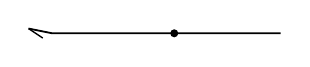
\begin{tikzpicture}[x=1cm,y=1cm]
\draw[line width=.65pt](-1.6,.06)--(-1.3,0)--(1.6,0);
\draw[line width=.5pt](-1.6,.06)--(-1.42,-.06);
\fill(.25,0)circle(1.45pt);
\end{tikzpicture}\end{center}
\Unclear{GELFAND-P000110}{affine-line}{A horizontal line with a marked point; no label at the point. At the left end a short downward slant: left arrowhead[?] / bend in the line. No arrowhead is visible on the right.}
\end{GelfandAdjacentEvidence}
\begin{GelfandAdjacentEvidence}{GELFAND-P000110}{182}

$k[x]$ — germs of polyn.s vanishing at the point 0, quotient — one-dim.
\SourceFigure{GELFAND-P000110}{polynomial-germs}{To the right of the drawing $k[x]$ — germs; on the next line of polyn.s vanishing at the point 0, quotient — one-dim.}
\end{GelfandAdjacentEvidence}
\begin{GelfandAdjacentEvidence}{GELFAND-P000110}{183}


\usetikzlibrary{decorations.pathmorphing}
\tikz[baseline=(title.base)]{\node[inner sep=0pt](title){Examination in hom. algebra — following Grothendieck.};\draw[decorate,decoration={snake,amplitude=.45pt,segment length=5pt}]([yshift=-2pt]title.south west)--([yshift=-2pt]title.south east);} — class test.
\SourceFigure{GELFAND-P000110}{exam-heading}{The wavy underline runs from Examination to Grothendieck. After it class, and test. is carried below without an underline.}
\end{GelfandAdjacentEvidence}
\begin{GelfandAdjacentEvidence}{GELFAND-P000110}{184}

\underline{Lemma 2.} $F\subset O_X^{n[?]}$ — direct $\sum$.
[Below, with an insertion sign: subsheaf.]
\Unclear{GELFAND-P000110}{lemma2-sum}{After direct, a separate $\sum$ / $\Sigma$ with a period to the right. The superscript of $O_X$ is n[?] / m-like; the small upper strokes merge. Subsheaf is inserted beneath F.}
\end{GelfandAdjacentEvidence}
\begin{GelfandAdjacentEvidence}{GELFAND-P000110}{185}

Let there be a section $s$ defined on $X_P$. Then for large $m$, $P^ms$ extends to the whole $X$.
\SourceFigure{GELFAND-P000110}{lemma2-extension}{The section s is defined on $X_P$. On the last line $P^ms$ extends to the whole X. A final period is visible.}
\end{GelfandAdjacentEvidence}



\begin{GelfandAdjacentEvidence}{GELFAND-P000111}{1}
\SourcePage{GELFAND-P000111}{72}
(also Hilbert's theorem).
\begin{equation*}\left(\frac{O_1\text{[?]}}{p^k},\ldots,\frac{O_i\text{[?]}}{p^k}\right)\end{equation*}
mult. by $p^k$, but this may not be a sect. of $O_X^n$.
\Unclear{GELFAND-P000111}{opening-numerators}{Rounded O-like signs in the numerators, with lower $1$ and $i$; their lower portions join the fraction bars. Readings $O$ / $Q$ are not fully distinguished. Beneath, $O_X^n$ and $O_X^n/F$.}
\end{GelfandAdjacentEvidence}
\begin{GelfandAdjacentEvidence}{GELFAND-P000111}{2}

$O_X^n/F\longrightarrow0$ already nepr.[?]
\Unclear{GELFAND-P000111}{quotient-last-word}{After already, a short joined entry source непр.[?] (nepr.[?]); its middle and final strokes merge densely. The abbreviation is not expanded. Before already, an arrow to a separate $0$.}
\end{GelfandAdjacentEvidence}
\begin{GelfandAdjacentEvidence}{GELFAND-P000111}{3}

Now it already suffices for the proof that the cohom. of $F\subset O_X^n$ are zeros.
$X$ — an aff. variety, $(X_{p_1},X_{p_2},\ldots,X_{p_i})$ a cover.
The cohomology of $X$ with coefficients in $F$ in this cover are zeros.

$22/\underline{\overline{XI}}$. \underline{I.M. Gelfand.}
[Crossed out: an illegible entry.] Bott, Chern Acta Math., 1965, \underline{114} $N=1$–$2$.
\Unclear{GELFAND-P000111}{bott-name-cancel}{Before Bott, a densely canceled entry with a Cyrillic Б-like beginning; its former letters are not established. A separate comma follows the cancellation.}
\end{GelfandAdjacentEvidence}
\begin{GelfandAdjacentEvidence}{GELFAND-P000111}{4}

\noindent\tikz[baseline=(title.base)]{\node[inner sep=0pt,outer sep=0pt](title){Theories of Nevanlinna for several variables.};\draw[decorate,decoration={snake,amplitude=.35mm,segment length=5mm}]([yshift=-2pt]title.south west)--([yshift=-2pt]title.south east);}
\SourceFigure{GELFAND-P000111}{nevanlinna-heading}{XI has separate over- and underlines; the surname with initials has a straight underline. The heading Theories of Nevanlinna for several variables. has a long wavy underline.}
\end{GelfandAdjacentEvidence}
\begin{GelfandAdjacentEvidence}{GELFAND-P000111}{5}

Picard's theorem, the more precise theorem of Nevanlinna:
one can estimate the number of zeros in a circle of radius $R$ (may be less).
$R_a$ — where it takes $a$.
\SourceFigure{GELFAND-P000111}{value-count-symbol}{Before the lower $a$, a large R-like letter with a slanting right leg. At right, a dash and where it takes $a$.}
\end{GelfandAdjacentEvidence}
\begin{GelfandAdjacentEvidence}{GELFAND-P000111}{6}

Most values are taken equ. often.
Defect — if not taken, then $1$; if less often, then a numer. char.
The $\sum$ of defects does not exceed two.
$\frac{a(z)}{b(z)}$ omits at most $2$ values.
$(a(z),b(z))$ a merom. fn. — a curve in $C^2$,
a value — a line (only the ratio matters).
This curve intersects all lines except, perhaps, two.
\noindent\tikz[baseline=(title.base)]{\node[inner sep=0pt,outer sep=0pt](title){Generalization.};\draw[decorate,decoration={snake,amplitude=.35mm,segment length=5mm}]([yshift=-2pt]title.south west)--([yshift=-2pt]title.south east);} In $3$-dim. space an entire curve $(a(z),b(z),c(z))$
intersects all planes passing through $0$, except, perhaps, three.
(In $n$-dim. a finite number.)

\noindent\tikz[baseline=(title.base)]{\node[inner sep=0pt,outer sep=0pt](title){For us this?};\draw[decorate,decoration={snake,amplitude=.35mm,segment length=5mm}]([yshift=-2pt]title.south west)--([yshift=-2pt]title.south east);}
$-y''+p(x)y=\lambda y$ — an eqn. on the int. $[0,\pi]$ with conditions
[At right:] $y(0)=0$, $y'(0)=0$.


[Crossed out: an illegible short sign.]
$\lambda$ [ne sushch.; abbreviation unexpanded], $y(0)=y(\pi)=0$ $\Rightarrow$ a countable number of eig. values.
\Unclear{GELFAND-P000111}{ode-endpoint-overwrite}{The right endpoint of the interval and the argument in the second entry $y(0)=y(\pi)=0$ are densely overwritten. The current sign has $\pi$-like strokes; the former entry is not established.}
\end{GelfandAdjacentEvidence}
\begin{GelfandAdjacentEvidence}{GELFAND-P000111}{7}

\SourceFigure{GELFAND-P000111}{initial-zero-derivative}{Two separate lines in the upper right field: $y(0)=0$ and $y'(0)=0$. Both final signs are oval, with a white centre.}
\end{GelfandAdjacentEvidence}
\begin{GelfandAdjacentEvidence}{GELFAND-P000111}{8}


\Unclear{GELFAND-P000111}{lambda-abbreviation}{Written source не сущ. (ne sushch.), with a period and following comma. The expansion of this abbreviation is not established on this line.}
\end{GelfandAdjacentEvidence}
\begin{GelfandAdjacentEvidence}{GELFAND-P000111}{9}

\Unclear{GELFAND-P000111}{lambda-prefix-cancel}{Immediately before $\lambda$, a short dense cancellation with a loop on the left and horizontal strokes. The former sign is unread.}
\end{GelfandAdjacentEvidence}
\begin{GelfandAdjacentEvidence}{GELFAND-P000111}{10}

Possibly, for most boundary conditions there is an eigenvalue
$y(0)=0$, $ay'(\pi)+by(\pi)=0$.
Consider the solution
\begin{center}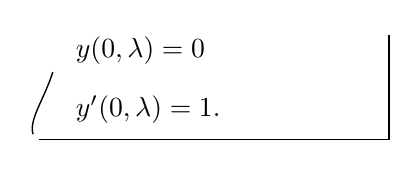
\begin{tikzpicture}[x=1cm,y=1cm]
\node[anchor=west]at(0,.75){$y(0,\lambda)=0$};
\node[anchor=west]at(0,0){$y'(0,\lambda)=1.$};
\draw[line width=.55pt](-.35,-.38)--(4.10,-.38)--(4.10,.95);
\draw[line width=.50pt](-.17,.48)..controls(-.27,.15)and(-.48,-.13)..(-.42,-.31);
\end{tikzpicture}\end{center}
It is analytic in $\lambda$.
\SourceFigure{GELFAND-P000111}{normalization-bracket}{Two lines $y(0,\lambda)=0$, $y'(0,\lambda)=1.$. Below them a horizontal line turns upward vertically at right. To the left of the second line a separate short curved stroke, unconnected to the lower line.}
\end{GelfandAdjacentEvidence}
\begin{GelfandAdjacentEvidence}{GELFAND-P000111}{11}

Eig. values — when
$ay'(\pi,\lambda)+by(\pi,\lambda)=0$ has a nonzero solution.
An analytic curve intersects almost[?] all [crossed out: an illegible word], lines,
and by Picard's theorem even infinitely many. (At most one)
\Unclear{GELFAND-P000111}{curve-line-cancellation}{Before all, a densely joined word: source почти (almost) / наши (our); its middle strokes are not fully distinguished. After all a long crossed-out entry; active lines follows at right. The next line ends (At most one).}
\end{GelfandAdjacentEvidence}
\begin{GelfandAdjacentEvidence}{GELFAND-P000111}{12}

How from general considerations do we obtain completeness (a curve in a function space) —
this has not been done.
One must prove a theorem in a Banach space — an analytic curve in a Banach space
(possibly, false)
[Crossed out: an illegible entry.] does not pass through a finite number of hyperplanes.
\Unclear{GELFAND-P000111}{banach-terminal-cancel}{Before does not pass, a separate dense cancellation with a long downward stroke. The former letters are not separated.}
\end{GelfandAdjacentEvidence}
\begin{GelfandAdjacentEvidence}{GELFAND-P000111}{13}

\begin{equation*}ay'(\pi,\lambda)-by(\pi,\lambda)=0.\end{equation*}
\SourceFigure{GELFAND-P000111}{terminal-boundary-minus}{In the last formula a separate horizontal minus stroke between $ay'$ and $by$. The derivative stroke at $y'$ is visible; both arguments are $(\pi,\lambda)$.}
\end{GelfandAdjacentEvidence}



\begin{GelfandAdjacentEvidence}{GELFAND-P000112}{1}
\SourcePage{GELFAND-P000112}{unlabelled}
The points into which it falls must be poln.[?]
\Unclear{GELFAND-P000112}{opening-final-word}{The line ends poln.[?] / polny; the middle strokes are densely joined, with a separate dot at the right. The ending is not established.}
\end{GelfandAdjacentEvidence}
\begin{GelfandAdjacentEvidence}{GELFAND-P000112}{2}

What is to be done for several complex variables?
All these are examples of sl.[?] analytic sheaves (in these terms both Borel's theorem and G. Weyl's theorem are formulated).
\Unclear{GELFAND-P000112}{opening-sheaf-word}{Before analytic there is a short sl.-like entry with a dense right stroke and a dot. The abbreviation is unexpanded.}
\end{GelfandAdjacentEvidence}
\begin{GelfandAdjacentEvidence}{GELFAND-P000112}{3}

There is no satisfactory theory analogous to Nevanlinna's theorems.
Distribution of the zeros of $n$ functions of $n$ variables — ?

§ 2. Characteristic classes (Chern classes)
\SourceFigure{GELFAND-P000112}{section-heading}{At the left are § and a separate $2$ with a dot. No underline is visible below the heading. At the right, (Chern classes).}
\end{GelfandAdjacentEvidence}
\begin{GelfandAdjacentEvidence}{GELFAND-P000112}{4}

$X$ — manifold, $E$ — vector bundle, $T=T(X)$ —
[Crossed out: unreadable entry.] tangent bundle.
\Unclear{GELFAND-P000112}{tangent-word-cancel}{Before the abbreviation for tangent a short prefix is densely crossed out; its individual earlier letters are not established.}
\end{GelfandAdjacentEvidence}
\begin{GelfandAdjacentEvidence}{GELFAND-P000112}{5}

$A^i(X)$ — sheaf of differential forms of order $i$.
$\sum A^i(X)=A(X)$ — a ring.
$d$ — differential in $A(X)$, $A(X,E)$ — sheaf of differential forms on $X$ with values in $E$.
\begin{equation*}A(X,E)=A(X)\otimes_{A^{0\text{[?]}}(E)}\Gamma(E).\end{equation*}
\Unclear{GELFAND-P000112}{tensor-base}{Below the first tensor sign, $A^{0\text{[?]}}(E)$: above $A$ is a round mark with a small opening, $0$ / $i$; in parentheses an E-like letter. Below the next tensor sign, a separate $A^0(X)$.}
\end{GelfandAdjacentEvidence}
\begin{GelfandAdjacentEvidence}{GELFAND-P000112}{6}

Notation.
\begin{equation*}\Gamma(E)\otimes_{A^0(X)}\Gamma(F)\longrightarrow\Gamma(E\otimes F)\end{equation*}
— this multiplication is denoted simply by a dot.
$E$ — vector bundle over $X$.
\underline{Definition.} A connection on $E$ is a differential operator $D$ on $\Gamma(E)$ satisfying the requirement:
\begin{equation*}
D:\Gamma(E)\longrightarrow\Gamma(T^*\otimes E),\qquad
D(fs)=df\cdot s+f\cdot Ds,\quad s\in\Gamma(E),\ f\in A^0(X).
\end{equation*}
\Unclear{GELFAND-P000112}{definition-title-overwrite}{In the underlined Definition. the middle letters are densely overwritten; the earlier strokes have not been read separately.}
\end{GelfandAdjacentEvidence}
\begin{GelfandAdjacentEvidence}{GELFAND-P000112}{7}

$T^*$ — kokas.[?] (!)
\Unclear{GELFAND-P000112}{cotangent-short-word}{After $T^*$, a short entry kokas. / konas.; the second consonant is densely joined to neighbouring strokes. A separate (!) is at the right.}
\end{GelfandAdjacentEvidence}
\begin{GelfandAdjacentEvidence}{GELFAND-P000112}{8}

Introduce local coordinates $\{s_i(x)\}$ in a neighbourhood $U$ — linear frames at each point $x$.
\SourceFigure{GELFAND-P000112}{local-frame-word}{Before the brace the words local coordinates are written; after the brace, linear frames. The handwritten word koordinat has a long upper arc at d and a separate final stroke.}
\end{GelfandAdjacentEvidence}
\begin{GelfandAdjacentEvidence}{GELFAND-P000112}{9}

\begin{equation*}Ds_i=\sum_{j=1}^n\theta_{ij}s_j.\end{equation*}
$\theta_{ij}$ — connection matrix $\theta(s,D)$.
Its values — differential forms.
\begin{equation*}K(s,D)=d\theta(s,D)-\theta(s,D)\wedge\theta(s,D).\end{equation*}
\SourceFigure{GELFAND-P000112}{curvature-minus}{After the first $\theta(s,D)$ is a separate horizontal minus stroke; between the following matrices is $\wedge$.}
\end{GelfandAdjacentEvidence}
\begin{GelfandAdjacentEvidence}{GELFAND-P000112}{10}

Not $0$, since this is a product of matrices
\begin{equation*}\sum_l\theta_{il}(s,D)\wedge\theta_{lj}(s,D).\end{equation*}
\SourceFigure{GELFAND-P000112}{curvature-indices}{Below the sum is a separate $l$; the first $\theta$ has lower $i,l$, the second lower $l,j$. Both factors have arguments $(s,D)$.}
\end{GelfandAdjacentEvidence}
\begin{GelfandAdjacentEvidence}{GELFAND-P000112}{11}

This exterior $2$-form is called the curvature.
$2$-forms commute with one another, so a $\det$ of forms makes sense.
The characteristic classes are called
\begin{equation*}C(E,D\text{[?]})=\operatorname{Det}\left(1+\frac{2\pi}{i}K(s,D)\right).\end{equation*}
\Unclear{GELFAND-P000112}{chern-second-argument}{In $C(E,D\text{[?]})$ the second argument is pale and round, with a dense left stroke; $D$ / a C-like letter.}
\end{GelfandAdjacentEvidence}
\begin{GelfandAdjacentEvidence}{GELFAND-P000112}{12}

\SourceFigure{GELFAND-P000112}{chern-prefactor}{In the fraction $2\pi$ is above the bar and $i$ below; before the fraction is a plus, and at the right $K(s,D)$.}
\end{GelfandAdjacentEvidence}
\begin{GelfandAdjacentEvidence}{GELFAND-P000112}{13}

These are closed $2$-forms.
[At the right:] Forms of different orders — and a collection of characteristic classes.
\SourceFigure{GELFAND-P000112}{closed-form-degree}{The bottom line literally has $2$-forms. A separate entry in the right margin: Forms of different orders — and a collection of characteristic classes.}
\end{GelfandAdjacentEvidence}



\begin{GelfandAdjacentEvidence}{GELFAND-P000113}{1}
\SourcePage{GELFAND-P000113}{73}
\begin{flushright}\tikz[baseline=(number.base)]{\node[inner sep=2pt](number){$73$};\draw([xshift=2pt]number.north east)--(number.north west)--(number.south west)--([xshift=2pt]number.south east);}\end{flushright}
Prove that $C$ does not depend on the choice of basis and is a closed form;
in fact it does not depend on the choice of connection either.
\noindent\tikz[baseline=(title.base)]{\node[inner sep=0pt,outer sep=0pt](title){Independence of the choice of basis.};\draw[decorate,decoration={snake,amplitude=.35mm,segment length=5mm}]([yshift=-2pt]title.south west)--([yshift=-2pt]title.south east);}
\begin{align*}
s'_i&=\sum A_{ij}s_j,\qquad s'=As;\\
Ds'&=dA\cdot s+A\theta(s,D)s,\\
Ds'&=\theta(s',D)s',\\
dA+A\theta(s,D)&=\theta(s',D)A.
\end{align*}
Substitute this into the definition of $K$.
\begin{center}\tikz[baseline=(eq.base)]{\node[inner sep=2pt](eq){$AK(s,D)=K(s',D)A$};\draw([xshift=-1mm,yshift=2mm]eq.south west)--([xshift=-1mm]eq.south west)--([xshift=1mm]eq.south east)--([xshift=1mm,yshift=2mm]eq.south east);}\end{center}
\begin{equation*}dA\cdot\theta(s,D)+Ad\theta(s,D)=d\theta(s,D)A+\theta(s',D)dA.\end{equation*}
\Unclear{GELFAND-P000113}{differentiated-frame-argument}{In the first $d\theta$ on the right the argument is $s$ without a separate prime. In the next $\theta$ the argument is $s'$ with a prime.}
\end{GelfandAdjacentEvidence}
\begin{GelfandAdjacentEvidence}{GELFAND-P000113}{2}

\SourceFigure{GELFAND-P000113}{differentiated-product-plus}{On the right between $d\theta(s,D)A$ and $\theta(s',D)dA$ is a separate plus with intersecting horizontal and vertical strokes.}
\end{GelfandAdjacentEvidence}
\begin{GelfandAdjacentEvidence}{GELFAND-P000113}{3}

``$A^{-1}KA^{+1\text{[?]}}$'' the same $\det$.
\Unclear{GELFAND-P000113}{conjugation-exponent}{Above the final $A$ are two dense raised strokes, currently $+1$[?]; the right vertical stroke is close to the closing quotation mark. No separate minus is visible.}
\end{GelfandAdjacentEvidence}
\begin{GelfandAdjacentEvidence}{GELFAND-P000113}{4}


\noindent\tikz[baseline=(title.base)]{\node[inner sep=0pt,outer sep=0pt](title){V. I. Arnold.};\draw[decorate,decoration={snake,amplitude=.35mm,segment length=5mm}]([yshift=-2pt]title.south west)--([yshift=-2pt]title.south east);}
Progress in the theory of singularities of differentiable mappings.
$f:M^m\longrightarrow N^n$ — $2$ manifolds.
\Unclear{GELFAND-P000113}{target-letter-overwrite}{In the target $N^n$ the capital letter is densely overwritten; the individual earlier strokes are unread.}
\end{GelfandAdjacentEvidence}
\begin{GelfandAdjacentEvidence}{GELFAND-P000113}{5}

$R^m\longrightarrow R^n$, $0\longrightarrow0$.
Whitney, Thom, Malgrange, B. Morin, Broadman, Mather,
(Haefliger, H. Levin, M. Mors).
\SourceFigure{GELFAND-P000113}{names-spellings}{The Latin list has Broadman, H. Levin and M. Mors; before Morin is a B-like capital.}
\end{GelfandAdjacentEvidence}
\begin{GelfandAdjacentEvidence}{GELFAND-P000113}{6}

The simplest case — Morse's theorem $n=1$ — critical points $df=0$.
$\leftarrow$ isolated for general position.
Determined by [Crossed out: an od...-like entry, continuation unreadable.] index and signature.
(Morse lemma) — a model for the theory.
\Unclear{GELFAND-P000113}{morse-cancel}{After the abbreviation for determined a short token with an od...-like beginning is cancelled. The middle and ending are densely covered by strokes.}
\end{GelfandAdjacentEvidence}
\begin{GelfandAdjacentEvidence}{GELFAND-P000113}{7}

Study the roughness[?] of singularities (if changed slightly, equivalent or not).
\Unclear{GELFAND-P000113}{depth-word-overwrite}{The beginning of the word after study is densely overwritten. The current reading is grubost'[?] (roughness), with a b-like upper arc and ending ost'; the earlier strokes are not established.}
\end{GelfandAdjacentEvidence}
\begin{GelfandAdjacentEvidence}{GELFAND-P000113}{8}

\begin{center}
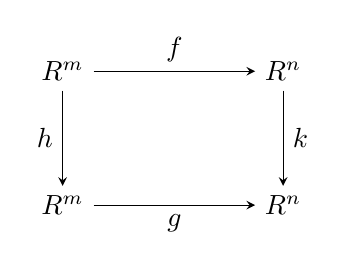
\begin{tikzpicture}[x=28mm,y=17mm,>=stealth]
\node (tl) at (0,1){$R^m$};\node (tr) at (1,1){$R^n$};
\node (bl) at (0,0){$R^m$};\node (br) at (1,0){$R^n$};
\draw[->](tl)--node[above]{$f$}(tr);
\draw[->](bl)--node[below]{$g$}(br);
\draw[->](tl)--node[left]{$h$}(bl);
\draw[->](tr)--node[right]{$k$}(br);
\end{tikzpicture}
\end{center}

$f,g$ are equivalent if obtained by a change of variables.
\SourceFigure{GELFAND-P000113}{coordinate-equivalence-square}{The upper and lower rows are $R^m\to R^n$, with $f$ above and $g$ below. Vertical arrows point down: $h$ on the left, $k$ on the right.}
\end{GelfandAdjacentEvidence}
\begin{GelfandAdjacentEvidence}{GELFAND-P000113}{9}


$d^2f$ without zeros — reducible to a quadratic form.
For the komp.[?] source manifold they form an everywhere pl.[?] open set.
\Unclear{GELFAND-P000113}{normal-form-density-word}{After for is a short komp.[?] / norm.; after everywhere a short pl.[?] / na. with a dot. The abbreviations are unexpanded. At the right, open set.}
\end{GelfandAdjacentEvidence}
\begin{GelfandAdjacentEvidence}{GELFAND-P000113}{10}

$R^m\longrightarrow R^1$ is solved.
Whitney's first result ($55$) $R^2\longrightarrow R^2$.
An example of singularities.
Singular points — rank of the differential $=1$ and they are of $2$ classes
(folds and cusps). They are structurally stable ($0$ can be avoided).
\noindent\tikz[baseline=(title.base)]{\node[inner sep=0pt,outer sep=0pt](title){Ordinary point};\draw[decorate,decoration={snake,amplitude=.35mm,segment length=5mm}]([yshift=-2pt]title.south west)--([yshift=-2pt]title.south east);}
\tikz[baseline=(cancel.base)]{\node[inner sep=0pt,outer sep=0pt](cancel){$(x,y)\longrightarrow(x,y)$};\draw([yshift=2pt]cancel.west)--([yshift=2pt]cancel.east);\draw([yshift=-3pt]cancel.west)--([yshift=-3pt]cancel.east);} $y_1=x_1$, $y_2=x_2$.
\Unclear{GELFAND-P000113}{ordinary-coordinate-cancel}{The entry $(x,y)\longrightarrow(x,y)$ is crossed out by two long horizontal lines. At the right, separately $y_1=x_1$, $y_2=x_2$.}
\end{GelfandAdjacentEvidence}
\begin{GelfandAdjacentEvidence}{GELFAND-P000113}{11}

\noindent\tikz[baseline=(title.base)]{\node[inner sep=0pt,outer sep=0pt](title){Fold point:};\draw[decorate,decoration={snake,amplitude=.35mm,segment length=5mm}]([yshift=-2pt]title.south west)--([yshift=-2pt]title.south east);}
[Crossed out: $(x,y)$[?], other strokes unread.] structurally stable.
\Unclear{GELFAND-P000113}{fold-coordinate-cancel}{Below the heading an $(x,y)$-like entry is densely crossed out; below the lower slanting strokes the individual letters are not separated.}
\end{GelfandAdjacentEvidence}
\begin{GelfandAdjacentEvidence}{GELFAND-P000113}{12}

\begin{equation*}\boxed{\begin{aligned}y_1&=x_1^2,\\y_2&\to x_2.\end{aligned}}\end{equation*}
\SourceFigure{GELFAND-P000113}{fold-normal-form-box}{Two lines in one frame. The first is $y_1=x_1^2$. In the second, between $y_2$ and $x_2$ is an arrow-like sign, a horizontal stroke with a point at the right.}
\end{GelfandAdjacentEvidence}
\begin{GelfandAdjacentEvidence}{GELFAND-P000113}{13}

\begin{center}
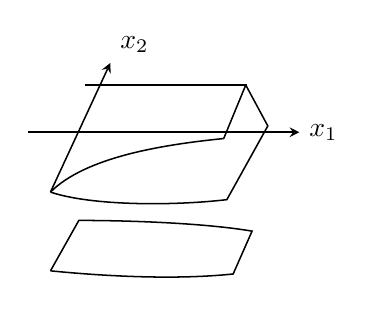
\begin{tikzpicture}[x=8mm,y=8mm,>=stealth,line width=.55pt]
\draw(.55,1.7)--(3.1,1.7)--(2.75,.85);
\draw(0,0)..controls(.65,-.22)and(1.95,-.22)..(2.8,-.12)--(3.45,1.05)--(3.1,1.7);
\draw(0,0)..controls(.55,.55)and(1.75,.75)..(2.75,.85);
\draw[->](-.35,.95)--(3.95,.95)node[right]{$x_1$};
\draw[->](0,0)--(.95,2.05)node[above right]{$x_2$};
\draw(0,-1.25)--(.45,-.45)..controls(1.35,-.45)and(2.5,-.5)..(3.2,-.62)--(2.9,-1.3)..controls(1.95,-1.4)and(.8,-1.33)..(0,-1.25);
\end{tikzpicture}
\end{center}
\SourceFigure{GELFAND-P000113}{fold-sketch}{Two separate oblique strips. The upper one has a curved front edge and an internal line; the $x_1$ axis points right, $x_2$ obliquely upward. The lower strip has no labels.}
\end{GelfandAdjacentEvidence}
\begin{GelfandAdjacentEvidence}{GELFAND-P000113}{14}

\noindent\tikz[baseline=(title.base)]{\node[inner sep=0pt,outer sep=0pt](title){Cusp point:};\draw[decorate,decoration={snake,amplitude=.35mm,segment length=5mm}]([yshift=-2pt]title.south west)--([yshift=-2pt]title.south east);}
\begin{center}\tikz[baseline=(cusp.base)]{\node[inner sep=2pt](cusp){$\begin{aligned}y_1&\mathrel{\overset{\text{[?]}}{\to}}x_1,\\y_2&=x_2^3-x_1x_2.\end{aligned}$};\draw(cusp.south west)--(cusp.south east);}\end{center}
\Unclear{GELFAND-P000113}{cusp-formula-minus}{At $y_1$ is a sign with two closely spaced strokes, $\to$ / $=$; at the right $x_1$. The second line is $y_2=x_2^3-x_1x_2$, with a separate minus. A long straight line is below both lines.}
\end{GelfandAdjacentEvidence}
\begin{GelfandAdjacentEvidence}{GELFAND-P000113}{15}

\begin{center}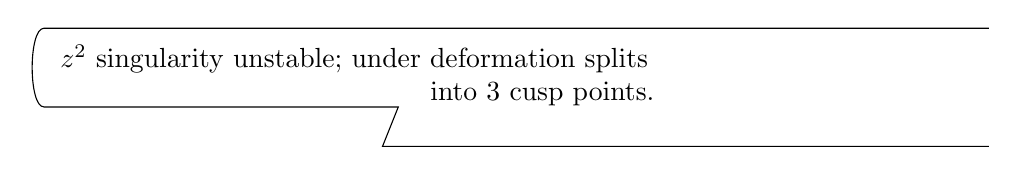
\begin{tikzpicture}[x=1mm,y=1mm]
\node[anchor=north west,inner sep=0pt,align=left,text width=116mm] at(2,-2){$z^2$ singularity unstable; under deformation splits\\\hspace*{47mm}into $3$ cusp points.};
\draw(120,0)--(0,0)..controls(-2,0)and(-2,-10)..(0,-10)--(45,-10)--(43,-15)--(120,-15);
\end{tikzpicture}\end{center}
\SourceFigure{GELFAND-P000113}{squared-map-callout}{At the right an entry is framed, open at the right edge, with a step in the lower outline. The text begins with $z^2$, and the next line has into $3$ cusp points.}
\end{GelfandAdjacentEvidence}
\begin{GelfandAdjacentEvidence}{GELFAND-P000113}{16}

Whitney's theorem: any [Crossed out: unreadable entry.] mapping is approximated by such ones.
\Unclear{GELFAND-P000113}{whitney-cancel}{Between any and the abbreviation for mapping is a short dense cancellation. The earlier letters are not established.}
\end{GelfandAdjacentEvidence}

Points of the $3$rd type are isolated, of the $2$nd type in $M^m$ a nonsingular
$1$-dimensional manifold; in $N$ it has singularities.


\begin{GelfandAdjacentEvidence}{GELFAND-P000114}{1}
\SourcePage{GELFAND-P000114}{unlabelled}
\noindent\tikz[baseline=(title.base)]{\node[inner sep=0pt,outer sep=0pt](title){Cusp.};\draw[decorate,decoration={snake,amplitude=.35mm,segment length=5mm}]([yshift=-2pt]title.south west)--([yshift=-2pt]title.south east);} Jacobian
\begin{equation*}\left|\begin{matrix}1&0\\-x_2&3x_2^2-x_1\end{matrix}\right|.\end{equation*}
$3x_2^2-x_1=0$ a parabola.
At $0$ a fold, but more complicated as a whole.
\SourceFigure{GELFAND-P000114}{origin-fold-wording}{At the right are separate lines At $0$ a fold, but / more complicated as a whole.}
\end{GelfandAdjacentEvidence}
\begin{GelfandAdjacentEvidence}{GELFAND-P000114}{2}

\begin{center}\begin{tikzpicture}[x=9mm,y=9mm,>=stealth,line width=.55pt]
\draw[->](-1.2,0)--(1.9,0)node[right]{$x_1$};
\draw[->](0,-1.35)--(0,1.65)node[above right]{$x_2$};
\draw(1.6,1.05)..controls(.5,.85)and(0,.55)..(0,0)..controls(0,-.6)and(.6,-1.05)..(1.55,-1.08);
\draw[->](4.6,0)--(7.4,0)node[right]{$y_1$};
\draw[->](6,-1.4)--(6,1.65)node[above left]{$y_2$};
\draw(6,0)..controls(6.45,0)and(6.95,.7)..(7.15,1.45);
\draw(6,0)..controls(6.45,0)and(6.9,-.6)..(7.1,-1.3);
\end{tikzpicture}\end{center}
\SourceFigure{GELFAND-P000114}{critical-curve-images}{At the left a parabola with vertex at the origin, $x_1$ right,$x_2$ up. At the right two branches with a common point,directed right; $y_1$ right,$y_2$ up.}
\end{GelfandAdjacentEvidence}
\begin{GelfandAdjacentEvidence}{GELFAND-P000114}{3}

Where does the parabola go?
[Crossed out: $y_2=\text{[?]}y_1^{3/2}$.]
\Unclear{GELFAND-P000114}{cusp-equation-cancel}{In the cancelled entry $y_2$,an equals sign and $y_1^{3/2}$ are visible. The coefficient and intervening strokes are densely covered.}
\end{GelfandAdjacentEvidence}
\begin{GelfandAdjacentEvidence}{GELFAND-P000114}{4}

$y_2=-Cy_1^{3/2}$.
\begin{center}\tikz[baseline=(eq.base)]{\node[inner sep=2pt](eq){$y_2^2=-y_1^3$};\draw([yshift=3mm]eq.south west)--(eq.south west)--(eq.south east)--([yshift=3mm]eq.south east);}\end{center}
$y_1>0$.
\SourceFigure{GELFAND-P000114}{negative-cusp-square}{The corner frame has $y_2^2=-y_1^3$,with a separate minus. Below and to the left is a separate $y_1>0$.}
\end{GelfandAdjacentEvidence}
\begin{GelfandAdjacentEvidence}{GELFAND-P000114}{5}

The mapping is not a fold on the whole parabola.
Away from the point $0$ a fold.
Consider lines parallel to the $x_2$ axis.
$x_1=\operatorname{const}\Rightarrow y_1=\operatorname{const}$.
$y_2=x_2^3-Cx_2$.
\SourceFigure{GELFAND-P000114}{cubic-parameter-line}{In the line $x_1=\operatorname{const}$ an arrow points to $y_1=\operatorname{const}$. Below is $y_2=x_2^3-Cx_2$,with a large C-like letter before $x_2$.}
\end{GelfandAdjacentEvidence}
\begin{GelfandAdjacentEvidence}{GELFAND-P000114}{6}

\begin{center}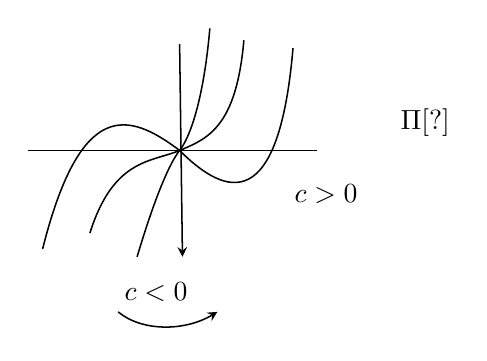
\begin{tikzpicture}[x=12mm,y=10mm,>=stealth,line width=.55pt]
\draw(-1.6,0)--(1.45,0);
\draw[->](0,1.35)--(.03,-1.35);
\draw(-1.45,-1.25)..controls(-1.05,.65)and(-.55,.5)..(0,0)..controls(.5,-.6)and(1.05,-.8)..(1.2,1.3);
\draw(-.95,-1.05)..controls(-.7,-.1)and(-.3,-.15)..(0,0)..controls(.3,.15)and(.6,.3)..(.68,1.4);
\draw(-.45,-1.35)..controls(-.25,-.55)and(-.1,-.15)..(0,0)..controls(.1,.15)and(.25,.6)..(.32,1.55);
\node at(1.55,-.55){$c>0$};\node at(-.25,-1.8){$c<0$};
\draw[->](-.65,-2.05)..controls(-.4,-2.3)and(.05,-2.3)..(.4,-2.05);
\node at(2.6,.35){$\Pi\text{[?]}$};
\end{tikzpicture}\end{center}
\Unclear{GELFAND-P000114}{cubic-family-sketch}{Several curves pass through the common intersection of the axes. At the right,next to the curve with turns,is $c>0$; below,$c<0$ and a curved arrow. At the right is a separate Cyrillic-P-/ $\Pi$-like mark,meaning unestablished.}
\end{GelfandAdjacentEvidence}
\begin{GelfandAdjacentEvidence}{GELFAND-P000114}{7}

$c<0$ the lines are mapped izom.[?] $c>0$.
\Unclear{GELFAND-P000114}{cubic-map-word}{After the abbreviation for mapped,a short izom.[?] / monot.-like word has densely joined middle strokes. The abbreviation is unexpanded.}
\end{GelfandAdjacentEvidence}
\begin{GelfandAdjacentEvidence}{GELFAND-P000114}{8}

\begin{center}\begin{tikzpicture}[x=9mm,y=9mm,>=stealth,line width=.55pt]
\draw[->](-1.5,0)--(1.8,0);\draw[->](0,-1.2)--(0,1.65);
\draw(1.2,1.25)..controls(.4,1.1)and(0,.55)..(0,0)..controls(0,-.55)and(.45,-1)..(1.25,-1.02);
\draw(-.65,-1.05)--(-.65,1.4);\draw(.8,-1.4)--(.8,1.65);
\node at(3.15,.45){$c>0$};
\draw(4.8,0)--(7.8,0);\draw(5.65,-1.15)--(5.65,1.15);
\draw(5.65,0)..controls(6.1,0)and(6.65,.55)..(7.15,1.1);
\draw(5.65,0)..controls(6.1,0)and(6.6,-.45)..(7.15,-1.3);
\draw(6.5,-1.45)--(6.5,1.5);\draw(6.9,-1.2)--(6.9,.85);
\draw(6.55,.6)..controls(6.35,.3)and(6.45,-.1)..(6.3,-.4);
\end{tikzpicture}\end{center}
\SourceFigure{GELFAND-P000114}{vertical-line-sketches}{At the left a parabola,axes and two separate verticals. At the right a pointed two-branch curve with several vertical strokes and a short curved internal line. Between the sketches is $c>0$.}
\end{GelfandAdjacentEvidence}
\begin{GelfandAdjacentEvidence}{GELFAND-P000114}{9}

A cusp occurs on all luchesnykh[?] branakh[?].
\Unclear{GELFAND-P000114}{ray-wording}{In the first disputed word a vertical diagram stroke crosses the middle: luchevykh / luchesnykh. In the second,the initial strokes are b-/g-like: branakh / granyakh. The full reading is not established.}
\end{GelfandAdjacentEvidence}
\begin{GelfandAdjacentEvidence}{GELFAND-P000114}{10}

\underline{Problem.}
[Crossed out: $z^2$[?] and unreadable strokes.]
$z\longrightarrow z^2+\varepsilon\overline z$ — general position.
$\varepsilon=0$ singularity at $0$; for $\varepsilon\ne0$ it moves,
there will be folds and cusps. And only this is stable.
\Unclear{GELFAND-P000114}{square-map-cancel}{After Problem. a z-like sign with an upper $2$ is cancelled; the right part of the entry is covered by long strokes.}
\end{GelfandAdjacentEvidence}
\begin{GelfandAdjacentEvidence}{GELFAND-P000114}{11}

\noindent\tikz[baseline=(title.base)]{\node[inner sep=0pt,outer sep=0pt](title){Scientific definition of a cusp.};\draw[decorate,decoration={snake,amplitude=.35mm,segment length=5mm}]([yshift=-2pt]title.south west)--([yshift=-2pt]title.south east);}
One of the known systems of invariants.
Rank $=r\text{[?]}$ — manifold $\Sigma_r$.
\Unclear{GELFAND-P000114}{rank-letter}{After the equals sign the letter is densely overwritten; currently $r$[?],with earlier round strokes unread separately. Below,similar signs occur at $\Sigma_r$ and in the sequence $r_1,r_2$.}
\end{GelfandAdjacentEvidence}
\begin{GelfandAdjacentEvidence}{GELFAND-P000114}{12}

$M^m$ is partitioned into manifolds.
\tikz[baseline=(cancel.base)]{\node[inner sep=0pt](cancel){Codim.};\draw([yshift=2pt]cancel.west)--([yshift=2pt]cancel.east);\draw([yshift=-2pt]cancel.west)--([yshift=-2pt]cancel.east);}

\begin{center}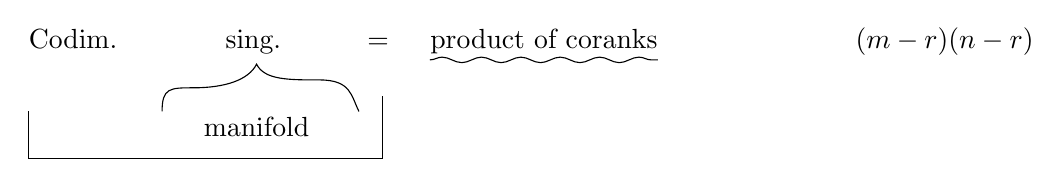
\begin{tikzpicture}[x=1mm,y=1mm,baseline=(codim.base)]
\node[anchor=base west,inner sep=0pt](codim) at(0,0){Codim.};
\node[anchor=base west,inner sep=0pt] at(25,0){sing.};
\node[anchor=base west,inner sep=0pt] at(43,0){$=$};
\node[anchor=base west,inner sep=0pt](prod) at(51,0){product of coranks};
\node[anchor=base west,inner sep=0pt] at(105,0){$(m-r)(n-r)$};
\node[inner sep=0pt] at(29,-10){manifold};
\draw(17,-8)..controls(17,-5)and(18,-5)..(21,-5)..controls(25,-5)and(28,-4)..(29,-2)..controls(30,-4)and(33,-4)..(37,-4)..controls(41,-4)and(41,-6)..(42,-8);
\draw(0,-8)--(0,-14)--(45,-14)--(45,-6);
\draw[decorate,decoration={snake,amplitude=.35mm,segment length=5mm}]([yshift=-2pt]prod.south west)--([yshift=-2pt]prod.south east);
\end{tikzpicture}\end{center}

(This is a question about independent minors of a rectangular matrix of rank $r$.)
\Unclear{GELFAND-P000114}{codimension-cancel}{The first Codim. is crossed out by long horizontal lines. Below,a separate repetition Codim. sing.}
\end{GelfandAdjacentEvidence}
\begin{GelfandAdjacentEvidence}{GELFAND-P000114}{13}

\SourceFigure{GELFAND-P000114}{rank-codimension-brackets}{Below sing. is a brace pointing up with the label manifold; below that,a long corner frame. Product of coranks has a wavy underline; at the right,$(m-r)(n-r)$.}
\end{GelfandAdjacentEvidence}
\begin{GelfandAdjacentEvidence}{GELFAND-P000114}{14}


$\Sigma_r$ — smooth manifolds in $R^m$; consider our mapping on the manifolds
themselves (parabola). Rank on these manifolds.
$\Sigma_{r_1,r_2}$, $r_2<r_1$ — submanifold — rank levels.
$\Sigma_{r_1,r_2,r_3}$.
To each [Crossed out: unreadable word.] singularity corresponds a set of numbers $r_1,r_2,r_3$.
\Unclear{GELFAND-P000114}{invariant-cancel}{After to each a long word,resembling osobennosti,is cancelled. Upper and lower horizontal strokes cover most letters.}
\end{GelfandAdjacentEvidence}

Invariant of a singularity $r_1\ge r_2\ge\cdots\ge0$.


\begin{GelfandAdjacentEvidence}{GELFAND-P000115}{1}
\SourcePage{GELFAND-P000115}{74}
Whitney sing.: \tikz[baseline=(sigma.base)]{\node[inner sep=0pt](sigma){$\Sigma_0$};\node[anchor=north,inner sep=0pt,font=\small] at([yshift=-1pt]sigma.south){ordinary};}.
The first index is the corank.
Cusp: $\Sigma_{10}$. It is proved that this is a manifold.
\SourceFigure{GELFAND-P000115}{sigma-examples}{For Whitney,$\Sigma_0$,with ordinary below it; for the cusp,$\Sigma_{10}$. At the right,The first index is the corank.}
\end{GelfandAdjacentEvidence}
\begin{GelfandAdjacentEvidence}{GELFAND-P000115}{2}

[Crossed out: D…]

For the partition in the space of Taylor-series segments. (Brodman) —
the old naive approach.
\Unclear{GELFAND-P000115}{top-cancel}{Before for the partition,a short cancelled entry; a Cyrillic-D-like beginning is visible,the other letters covered by strokes.}
\end{GelfandAdjacentEvidence}
\begin{GelfandAdjacentEvidence}{GELFAND-P000115}{3}


It is known that $\Sigma$ is not a complete classification.
(There is an example $R^9\longrightarrow R^9$.)
\underline{General theory.} Consider the space of Taylor series.
($3$ classes — $C^\infty$, analytic, formal power series.)
[At the right:] $R^m\longrightarrow R^n$; $C^\infty$ has Taylor series.
\begin{equation*}y=\sum_{k\mathrel{\overset{\text{[?]}}{\ge}}0}a_kx^k,\qquad a_k\text{ — a vector},\quad k=(k_1,\ldots,k_m).\end{equation*}
\Unclear{GELFAND-P000115}{multiindex-series}{Below the sum,$k\ge0$[?] / $k>0$; the small strokes of the sign are joined. At the right,$a_k$ is a vector,$k=(k_1,\ldots,k_m)$.}
\end{GelfandAdjacentEvidence}
\begin{GelfandAdjacentEvidence}{GELFAND-P000115}{4}

Local theories.
$C^\infty$ — the most difficult, analytic — the most interesting, formal series —
the simplest.
Mappings are equivalent if there is a change.
A partition into pieces arises — a stratification. Study of this partition.
\begin{center}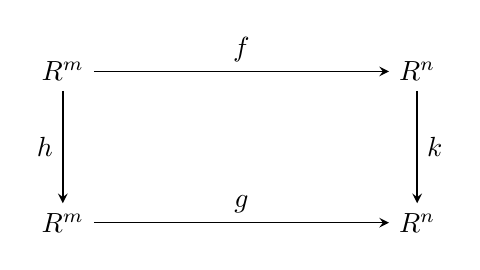
\begin{tikzpicture}[x=15mm,y=12mm,>=stealth,line width=.55pt]
\node(A)at(0,0){$R^m$};\node(B)at(3,0){$R^n$};
\node(C)at(0,-1.6){$R^m$};\node(D)at(3,-1.6){$R^n$};
\draw[->](A)--node[above]{$f$}(B);
\draw[->](C)--node[above]{$g$}(D);
\draw[->](A)--node[left]{$h$}(C);
\draw[->](B)--node[right]{$k$}(D);
\end{tikzpicture}\end{center}

$h,k$ — formal diffeomorphisms ($1$st terms with Jacobian $\ne0$).
\SourceFigure{GELFAND-P000115}{formal-equivalence-square}{Two rows $R^m\to R^n$: above,$f$; below,$g$; vertical arrows down,$h$ on the left,$k$ on the right.}
\end{GelfandAdjacentEvidence}
\begin{GelfandAdjacentEvidence}{GELFAND-P000115}{5}


There is an example ($>9$) with infinitely many invariants.
\noindent\tikz[baseline=(title.base)]{\node[inner sep=0pt](title){Thom};\draw[decorate,decoration={snake,amplitude=.35mm,segment length=5mm}]([yshift=-2pt]title.south west)--([yshift=-2pt]title.south east);\draw[->]([xshift=-8mm,yshift=6mm]title.west)--([xshift=-6mm,yshift=-1mm]title.west); } proved that in the space of power series a part of infinite codimension is singled out,
that the rest are stable in the topological sense.
\Unclear{GELFAND-P000115}{headings-and-arrow}{General theory. has a straight underline,with middle letters overwritten. Thom has a wavy underline; at the left,a short arrow down. Earlier strokes of the name cannot be read separately.}
\end{GelfandAdjacentEvidence}
\begin{GelfandAdjacentEvidence}{GELFAND-P000115}{6}

(Thom's invariants in $R^9$ are invariants of smooth,but not nepr.[?])
\Unclear{GELFAND-P000115}{tom-invariant-abbreviation}{The final abbreviation is nepr. / nerp.; the joined middle strokes do not give an unambiguous letter order.}
\end{GelfandAdjacentEvidence}
\begin{GelfandAdjacentEvidence}{GELFAND-P000115}{7}

(Thom does not want to publish the proof,he is working on biology.
The proof was recounted,for a whole year,but nobody understood it:
Malgrange, Cartan, Arnold and others.)
$\bigcup X_\gamma+X_\infty$, $X_\gamma$ singularities stable in the topological sense.
\SourceFigure{GELFAND-P000115}{strata-union-sign}{Before $X_\gamma$ is a large union sign without a lower index; between $X_\gamma$ and $X_\infty$ is a separate plus.}
\end{GelfandAdjacentEvidence}
\begin{GelfandAdjacentEvidence}{GELFAND-P000115}{8}

For some dimensions Thom's analytic difficulties do not arise.
(Singularities differentially stable.)
Apparently the problem is solved where there is
[Crossed out: unreadable word.]
a classification. (In small dimensions.)
\Unclear{GELFAND-P000115}{classification-cancel}{Between there is and classification,a long cancelled entry covered by several horizontal strokes.}
\end{GelfandAdjacentEvidence}
\begin{GelfandAdjacentEvidence}{GELFAND-P000115}{9}

There are $\Sigma$ that are differentially stable $\Sigma_{1,\ldots,1,0}$.
Not all $\Sigma$ are differentially stable.
Another result of Mother. (Milnor's student.)
\SourceFigure{GELFAND-P000115}{mather-source-spelling}{The name has a round $o$: Mother. In the lower repetition,Mother′a.}
\end{GelfandAdjacentEvidence}
\begin{GelfandAdjacentEvidence}{GELFAND-P000115}{10}

$\delta y=\varphi(x)$.
$h(x)$ — variation in $X$ — a vector field.
\begin{center}\begin{tikzpicture}[x=12mm,y=12mm,>=stealth,line width=.55pt]
\draw(-1.2,0)--(2.15,0);\draw(0,-.7)--(0,1.8);
\draw(.25,.85)..controls(.65,1.55)and(1.15,1.8)..(1.7,1.45);
\draw(.25,.45)..controls(.6,1.25)and(1.15,1.4)..(1.65,.9);
\node[right]at(1.65,.9){$f(x)$};
\draw[->](.65,-.3)--(1.65,-.3)node[below]{$h(x)$};
\draw[->](-.75,.4)--(-.75,1.35)node[left]{$k(y)$};
\end{tikzpicture}\end{center}
\SourceFigure{GELFAND-P000115}{variation-sketch}{Crossing axes and two nearby arcs above the horizontal,with $f(x)$ at the lower arc. A separate horizontal arrow right below the axis is labelled $h(x)$,and a vertical arrow up at the left,$k(y)$.}
\end{GelfandAdjacentEvidence}
\begin{GelfandAdjacentEvidence}{GELFAND-P000115}{11}

Change of variables — the function changes by $f'(x)h(x)+k(y)$.
In the $1$st approximation one must solve the equation
\begin{equation*}\varphi(x)=f'(x)h(x)+k(y).\end{equation*}
\Unclear{GELFAND-P000115}{linear-k-overwrite}{In the first formula,$k(y)$ is densely overwritten; below,in a separate equation,is a clean $k(y)$. The earlier strokes of the first letter are unread.}
\end{GelfandAdjacentEvidence}
\begin{GelfandAdjacentEvidence}{GELFAND-P000115}{12}

The corresponding theorem says that for stability it is necessary and sufficient
that the corresponding linear problem be solvable. ($\forall\varphi(x)$)
(sek. verkhnikh.[?] sheaves[?])
\Unclear{GELFAND-P000115}{sheaf-parenthetical}{The beginning is sek.; the next word is verkhnikh.[?] / ver…nikh.-like,the full reading unestablished. The last word is puchki / puchka.}
\end{GelfandAdjacentEvidence}
\begin{GelfandAdjacentEvidence}{GELFAND-P000115}{13}

(This is Mother's $1$st theorem. Moreover,it suffices for $\varphi(x)$
given by a polynomial of degree equal to dim. $\ell\text{[?]}$.)
\Unclear{GELFAND-P000115}{jet-power-overwrite}{After dim.,a densely overwritten sign,$\ell$- / $N$-like; earlier strokes are covered.}
\end{GelfandAdjacentEvidence}

But the proof is incorrect.
Modern technique (nonlinear functions in $C^\infty$ spaces).
All dimensions for which everything is good have been found.
$R^2\longrightarrow R^2,R^3$ (Whitney); in $R^4$ unknown,
in $R^5$ already known (there are no singularities at all any more).
Immersion (immersion).
For $m=n$ up to $8$ all mappings are stable (approx.).


\begin{GelfandAdjacentEvidence}{GELFAND-P000116}{1}
\SourcePage{GELFAND-P000116}{unlabelled}
Thom — a continuous invariant (stable).
It is not topological — it is an invariant of smooth mappings.
Under continuous deformation one can deform them.
29/\underline{XI}. \underline{Once} \underline{again} \underline{about[?]} \underline{characteristic} \underline{classes.}
[Crossed out: unreadable word.]

(I. M. Gelfand.)
\Unclear{GELFAND-P000116}{heading-cancel}{After classes.,a long densely cancelled entry; the letters are covered by horizontal strokes.}
\end{GelfandAdjacentEvidence}
\begin{GelfandAdjacentEvidence}{GELFAND-P000116}{2}


\Unclear{GELFAND-P000116}{heading-and-underlines}{Before characteristic,a round densely overwritten letter,o[?],with its own straight underline. Parts of the heading are underlined separately. Beautiful observation. and Classification: below have wavy underlines.}
\end{GelfandAdjacentEvidence}
\begin{GelfandAdjacentEvidence}{GELFAND-P000116}{3}

Consider $E$ over $X$,a connection $D:\Gamma(E)\to\Gamma(T^*\otimes E)$.
\tikz[baseline=(f.base)]{\node[inner sep=0pt](f){$f$};\node[anchor=north,inner sep=0pt,font=\small](label)at([yshift=-3mm]f.south){function};\draw(f.south)--(label.north);} $\in A^0$, $s\in\Gamma(E)$ $\Rightarrow$
$D(fs)=f\cdot Ds+df\cdot s$.
[At the right:] (Here $T$ is the tang.[?] bundle.)
\Unclear{GELFAND-P000116}{tangent-abbreviation-cancel}{Before and at the beginning of kas.,a dense correction; the earlier strokes cannot be read separately.}
\end{GelfandAdjacentEvidence}
\begin{GelfandAdjacentEvidence}{GELFAND-P000116}{4}

[In the margin:] \tikz[baseline=(two.base)]{\node[draw,circle,inner sep=1pt](two){$2$};}
More precisely — tensor product in $A\otimes_{A^0}\Gamma(E)$.
\SourceFigure{GELFAND-P000116}{tensor-product-and-annotations}{Below $f$ is the label function,joined to the letter by a short stroke. In the tensor product,$A^0$ is below $\otimes$. In the right margin,$2$ is circled.}
\end{GelfandAdjacentEvidence}
\begin{GelfandAdjacentEvidence}{GELFAND-P000116}{5}

Cartan's moving frame (locally): $s_i$ $(i=1,\ldots,n)$,
$n$ — dim.[?] of the fibre.

Linearly independent at $\forall$ point.
\Unclear{GELFAND-P000116}{rank-word-overwrite}{In $n$ — dim. of the fibre,the abbreviation for dimension is densely overwritten; earlier letters are covered.}
\end{GelfandAdjacentEvidence}
\begin{GelfandAdjacentEvidence}{GELFAND-P000116}{6}


$D(s_i)=\sum\theta_{ij}s_j$,coefficients from $A^1$ (forms).
$\|\theta_{ij}\|$ is called the connection matrix (in Cartan — $\omega$).
\SourceFigure{GELFAND-P000116}{frame-section-symbols}{For sections an s-like letter recurs: $s\in\Gamma(E)$,$s_i$,$s_j$; below,$s=(s_1,\ldots,s_n)$. The initial $D$ in $D(fs)$ is overwritten.}
\end{GelfandAdjacentEvidence}
\begin{GelfandAdjacentEvidence}{GELFAND-P000116}{7}

\begin{equation*}
\|K_{ij}\|=K(s,D)=d\theta(s,D)-\theta(s,D)\wedge\theta(s,D),
\qquad s=(s_1,\ldots,s_n).
\end{equation*}
(This is a matrix.) (Matrix product,but the product is exterior.)
The form
\begin{equation*}C(E,D)=\det\left|I+\frac{i}{2\pi}K(s,D)\right|.\end{equation*}
\SourceFigure{GELFAND-P000116}{chern-factor-reversal}{In the determinant,before $K(s,D)$,a fraction with $i$ in the numerator and $2\pi$ in the denominator.}
\end{GelfandAdjacentEvidence}
\begin{GelfandAdjacentEvidence}{GELFAND-P000116}{8}

The entries are forms of even order,they commute and one can take $\det$.
A $\sum$ of forms of different orders. These are the characteristic classes
associated with the given bundle. This does not depend on the choice of connection.
[Idea of the proof according to Gelfand: closedness and this are proved,$\theta\text{[?]}$ changed.

The form no longer depends on the connection,$\int$ can be expressed through
$\int$ over the boundary. A variation of the connection inside has no effect.]
\Unclear{GELFAND-P000116}{proof-theta-overwrite}{Before changed,a dense $\theta$- / paragraph-like sign,with a round upper and dense lower stroke.}
\end{GelfandAdjacentEvidence}
\begin{GelfandAdjacentEvidence}{GELFAND-P000116}{9}


It does not depend on the choice of frame.
Bianchi identity:
\begin{equation*}dK(s,D)=-[K(s,D),\theta(s,D)].\end{equation*}
(Derivative of the curvature tensor.)
\SourceFigure{GELFAND-P000116}{curvature-and-bianchi}{The curvature formula has a minus before $\theta\wedge\theta$. The Bianchi identity has a minus before the commutator; the order inside the brackets is $K(s,D),\theta(s,D)$.}
\end{GelfandAdjacentEvidence}
\begin{GelfandAdjacentEvidence}{GELFAND-P000116}{10}

\noindent\tikz[baseline=(title.base)]{\node[inner sep=0pt,outer sep=0pt](title){Beautiful observation.};\draw[decorate,decoration={snake,amplitude=.35mm,segment length=5mm}]([yshift=-2pt]title.south west)--([yshift=-2pt]title.south east);}
$g_{\alpha\beta}(x)$ — a Riemannian metric,we shall take all successive
derivatives of $g_{\alpha\beta}(x)$ and form tensors from them.
How does one find all tensors that can be formed from $g_{\alpha\beta}(x)$?
\noindent\tikz[baseline=(title.base)]{\node[inner sep=0pt,outer sep=0pt](title){Classification:};\draw[decorate,decoration={snake,amplitude=.35mm,segment length=5mm}]([yshift=-2pt]title.south west)--([yshift=-2pt]title.south east);} they are functions of the curvature tensor and all covariant
derivatives of the curvature tensor (of any order) (algebraic expressions in them).
But what algebraic relations? (Between first covariant derivatives — the Bianchi identity.)
Introduce normal coordinates (po[?] geodesics) mr.[?] bundle.
\Unclear{GELFAND-P000116}{normal-coordinate-wording}{At the beginning of the parentheses,a short po[?]-like word. After the parentheses,mr.[?] / metr.-like abbreviation before bundle; the full reading is unestablished.}
\end{GelfandAdjacentEvidence}
\begin{GelfandAdjacentEvidence}{GELFAND-P000116}{11}

\begin{equation*}\begin{aligned}
g_{\alpha\beta}(x)&=g_{\alpha\beta}(0)+g_{\alpha\beta,\delta\delta}x^\delta x^\delta\\
&\quad+g_{\alpha\beta,\delta\delta\varepsilon}\text{[?]}x^\delta x^\delta x^\varepsilon.
\end{aligned}\end{equation*}
\Unclear{GELFAND-P000116}{normal-metric-indices}{In the second term,two $\delta$-like letters in the subscripts and at both $x$'s. In the third,the subscripts are $\delta\delta\varepsilon$[?] / $\gamma\delta\varepsilon$,with the middle letter overwritten; the superscripts are also $\delta$- / $\gamma$-like,the last $\varepsilon$.}
\end{GelfandAdjacentEvidence}

In a normal system they are all tensors.
This system of tensors,and here the algebraic relations are simpler.


\begin{GelfandAdjacentEvidence}{GELFAND-P000117}{1}
\SourcePage{GELFAND-P000117}{75}
\underline{V. I. Arnold.} Stable flow.
$\dot x=f(x,C)$; $g^t$ — a group of diffeomorphisms.
There are chemical and biological models (Thom).
$x$ \tikz[x=1mm,y=1mm,baseline=-.3mm]{\draw(0,0)--(3,0)--(1.5,2.7)--cycle;\fill(1.5,.9)circle(.25);} sums of substances,$c$ — a parameter.
\SourceFigure{GELFAND-P000117}{flow-definition-marks}{Between $x$ and sums of substances,a triangle with a dot inside. The right parameter label uses lowercase $c$,the equation uppercase $C$.}
\end{GelfandAdjacentEvidence}
\begin{GelfandAdjacentEvidence}{GELFAND-P000117}{2}

Consider one (stable).
A number of kogrubost[?] is introduced.
\begin{center}\begin{tikzpicture}[x=13mm,y=11mm,>=stealth,line width=.55pt]
\node(A)at(0,0){$X$};\node(B)at(2,0){$X$};\node(C)at(0,-1.5){$X$};\node(D)at(2,-1.5){$X$};
\draw[->](A)--node[above]{$g^t\text{[?]}$}(B);\draw[->](C)--node[above]{$h\text{[?]}$}(D);
\draw[->](A)--(C);\draw[->](B)--(D);
\end{tikzpicture}\end{center}
\Unclear{GELFAND-P000117}{flow-conjugacy-square}{Four $X$'s; above the upper horizontal arrow,an overwritten $g^t$[?],above the lower,an h-like letter. Horizontals right,verticals down,with no labels at the verticals.}
\end{GelfandAdjacentEvidence}
\begin{GelfandAdjacentEvidence}{GELFAND-P000117}{3}

Stable if for $\forall$ nearby $h$ there is a perturbation of $X$.
One cannot consider only stable ones (when parameters change,one may pass through nonstable parameters).
$(x,C)$ — a point of kogrubost[?] $1$,if for nearby parameter values
stable,etc.
As a mapping $X\times C\longrightarrow X\times C$,stable.
(How many terms of the Taylor series must be taken.)
A centre — an infinite degree of nonstability.
\begin{center}\tikz[x=1mm,y=1mm]{\draw(0,0)circle(5);\draw(0,0)circle(3.4);\draw(0,0)circle(1.5);}\end{center}
\SourceFigure{GELFAND-P000117}{center-circles}{Next to the entry about a centre,three nested closed round lines. They have no labels.}
\end{GelfandAdjacentEvidence}
\begin{GelfandAdjacentEvidence}{GELFAND-P000117}{4}

Thom's theorem on germs of Taylor series
$\vartheta=\vartheta^\infty+\bigcup_\gamma\vartheta^\gamma$.

[Below the formula:] \underline{\underline{codim. $\infty$}}
\Unclear{GELFAND-P000117}{jet-strata-symbol}{The recurring letter is $\vartheta$[?] / $\theta$ / O-like,with a large upper loop; the superscripts are $\infty$ and gamma-like.}
\end{GelfandAdjacentEvidence}
\begin{GelfandAdjacentEvidence}{GELFAND-P000117}{5}


\SourceFigure{GELFAND-P000117}{jet-codimension-annotation}{Below the formula,a separate annotation codim. $\infty$,underlined twice.}
\end{GelfandAdjacentEvidence}
\begin{GelfandAdjacentEvidence}{GELFAND-P000117}{6}

In $\vartheta^\gamma$,an open subset of finite negrub.[?]
In $\vartheta^\gamma$ singularities are described by finitely many parameters,inside
[Crossed out: unreadable short token.]

$\vartheta^\gamma$,all are diffeomorphic. (Tr-ie for differential equations.)
\Unclear{GELFAND-P000117}{inside-stratum-cancel}{After inside,a short dense cancellation; separately at its left,another short horizontal stroke.}
\end{GelfandAdjacentEvidence}
\begin{GelfandAdjacentEvidence}{GELFAND-P000117}{7}


In $\vartheta^\infty$,complete chaos (but they are of finite codim.[?]).
All $1$-parameter ones are in $\vartheta^\infty$.
\Unclear{GELFAND-P000117}{nongenericity-wording}{In the first lines after number and point,a ko-/negrubosti-like word; literally kogrubosti[?]. In the right annotation,finite negrub.[?]; in the lower parentheses,finite korazm.[?] / kogrub.-like abbreviation. Initial and middle strokes are joined.}
\end{GelfandAdjacentEvidence}
\begin{GelfandAdjacentEvidence}{GELFAND-P000117}{8}

For self-mappings,the invariants are unknown.
(F. Bendixson's theorem:

$\frac{dy}{dx}=\frac{P}{Q}$ on $CP^2$,then by finitely many $\sigma$-processes
one reaches Bendixson singular points
$x^p\frac{dy}{dx}=\lambda y+P(x,y)$.
Already an invariant relative to $\sigma$-processes.
A $\sigma$-process — substitute $\frac{y\text{[?]}}{x}$ \tikz[x=1mm,y=1mm,>=stealth]{\draw[->](0,4)..controls(2,1)and(2,-1)..(-1,-3);}. 

For $3$ variables unknown. On a birationally equivalent manifold,simple singular points.
Acta Math. $1901$.)
\Unclear{GELFAND-P000117}{bendixson-prefix}{At the beginning of the parentheses,a separate F-like Latin letter with a dot. The beginning of the next word is overwritten; the current reading is theorem.}
\end{GelfandAdjacentEvidence}
\begin{GelfandAdjacentEvidence}{GELFAND-P000117}{9}

\Unclear{GELFAND-P000117}{sigma-substitution}{The numerator is $y$[?] / h-like,densely overwritten; the denominator $x$. Beside it,a short pointer bent down.}
\end{GelfandAdjacentEvidence}
\begin{GelfandAdjacentEvidence}{GELFAND-P000117}{10}


\underline{On the Weierstrass preparation theorem.} (Malgrange.)
\begin{equation*}P(y)=y^n+\sum_{i=1}^{n-1}y^ia_i(x,z).\end{equation*}
\Unclear{GELFAND-P000117}{polynomial-argument-cancel}{In the first argument of $a_i$,a dense cancellation,currently $x$[?]. Below,a separate clean $a_i(x,z)$.}
\end{GelfandAdjacentEvidence}
\begin{GelfandAdjacentEvidence}{GELFAND-P000117}{11}

\SourceFigure{GELFAND-P000117}{weierstrass-constant-term}{The first sum's lower limit is explicitly $i=1$,the upper $n-1$.}
\end{GelfandAdjacentEvidence}
\begin{GelfandAdjacentEvidence}{GELFAND-P000117}{12}

Distinguished polynomial \underline{$a_i(x,z)$},$a_i(0,0)=0$.
\Unclear{GELFAND-P000117}{a-zero-overwrite}{The second $0$ in $a_i(0,0)=0$ is densely overwritten; earlier strokes are covered.}
\end{GelfandAdjacentEvidence}
\begin{GelfandAdjacentEvidence}{GELFAND-P000117}{13}

Spät Ruckert.
\SourceFigure{GELFAND-P000117}{headings-and-names}{The name V. I. Arnold. is underlined,the next line Stable flow. separate. The heading On the Weierstrass preparation theorem. is underlined; below,$a_i(x,z)$ is also underlined. The Latin entry is Spät Ruckert.}
\end{GelfandAdjacentEvidence}
\begin{GelfandAdjacentEvidence}{GELFAND-P000117}{14}

$P(y,x,z)$; $y$ — one variable,
$x=(x_1,\ldots,x_m)$,$z=(z_1,\ldots,z_n)$ — spare ones.
$3$ forms ($C^\infty$,analytic,formal series).
\begin{equation*}f(x,y,z)=P(y,x,z)\tikz[baseline=(q.base)]{\node[inner sep=0pt](q){$Q(y,x,z)$};\node[draw,anchor=north,inner sep=2pt,font=\small](caption)at([yshift=-5mm]q.south){$\text{of the same class}$};\draw(q.south east)--(caption.north east);}+\sum_0^{n-1}y^ib_i(x,z).\end{equation*}
\SourceFigure{GELFAND-P000117}{division-quotient-annotation}{Below $Q(y,x,z)$,a frame with the label of the same class,joined to the right of the entry by a short line. The remainder sum's lower limit is $0$.}
\end{GelfandAdjacentEvidence}
\begin{GelfandAdjacentEvidence}{GELFAND-P000117}{15}

(Division is possible.) (One can do this on relative sets.)
[[This works for Bendixson: the process must be finite.]]
The quotient by the ideal generated by $P$ has finite dimension
[Crossed out: unreadable token.] over

[Below at the right:] the corresponding ring.
\Unclear{GELFAND-P000117}{ideal-dimension-cancel}{Before over,a short entry is densely cancelled; the hidden letters are unread.}
\end{GelfandAdjacentEvidence}
\begin{GelfandAdjacentEvidence}{GELFAND-P000117}{16}


\SourceFigure{GELFAND-P000117}{ideal-over-line}{Over stands at the end of the upper line. The corresponding ring. is below at the right,at the end of the next line.}
\end{GelfandAdjacentEvidence}
\begin{GelfandAdjacentEvidence}{GELFAND-P000117}{17}

(Malgrange: for $C^\infty$ this is also true,but there is no longer uniqueness.)
$1)$ Let $P$ nearby have $n$ real roots —
by interpolation it will be $C^\infty$,but (the approximating polynomial by Lagrange's
theorem is uniquely determined by the description — this is difficult).
\begin{center}\begin{tikzpicture}[x=10mm,y=10mm,>=stealth,line width=.55pt]
\draw[->](-1,0)--(2.1,0)node[below right]{$x$};\draw[->](0,-1)--(0,1.8)node[above left]{$y$};
\draw(0,0)..controls(.3,.2)and(.5,1)..(.6,1.55);
\draw(0,0)..controls(.4,.25)and(.8,.85)..(1.05,1.5);
\draw(0,0)..controls(.55,.2)and(1.1,.65)..(1.6,1);
\node[anchor=west]at(2,1.1){$P(x,y)=0$};
\end{tikzpicture}\end{center}
\SourceFigure{GELFAND-P000117}{real-root-branches}{Axes:$x$ right,$y$ up. Three separate branches leave the origin into the first quadrant. At the right,the label $P(x,y)=0$.}
\end{GelfandAdjacentEvidence}
\begin{GelfandAdjacentEvidence}{GELFAND-P000117}{18}

$2)$ [Crossed out: $f(y,x)$-like entry.]

\tikz[baseline=(flat.base)]{\node[inner sep=0pt](flat){$f(x)$};\node[anchor=base west,inner sep=0pt](word)at([xshift=4mm]flat.base east){flat};\draw([yshift=-2pt]flat.south west)..controls([yshift=-4pt]flat.south)and([yshift=-4pt]flat.south east)..([xshift=2mm,yshift=-2pt]flat.south east)--([xshift=2mm,yshift=1mm]flat.south east)--([yshift=-2pt]word.south west)--([yshift=-2pt]word.south east);} at $0$ (all derivatives $0$).
\Unclear{GELFAND-P000117}{flat-f-cancel}{In the cancelled entry,the arguments look like y,x. Below it,a clean $f(x)$. The first division formula ends with a separate $+f(x)$.}
\end{GelfandAdjacentEvidence}
\begin{GelfandAdjacentEvidence}{GELFAND-P000117}{19}


Divide by $y^2+x^2$. Trivial answer.
\begin{equation*}f(x)=(y^2+x^2)\cdot0+f(x).\end{equation*}
\begin{center}\begin{tikzpicture}[baseline=(left.base),line width=.55pt]
\node[inner sep=0pt](left){$f(x)=(y^2+x^2)$};
\node[anchor=base west,inner sep=1pt](fraction)at([xshift=5mm]left.base east){$\displaystyle\frac{f(x)}{y^2+x^2}$};
\node[anchor=base west,inner sep=0pt](zero)at([xshift=8mm]fraction.base east){$+0$};
\draw(fraction.center)ellipse[x radius=11mm,y radius=8mm];
\draw([xshift=11mm]fraction.center)..controls([xshift=20mm,yshift=5mm]fraction.center)and([xshift=30mm,yshift=4mm]fraction.center)..([xshift=40mm,yshift=4mm]fraction.center);
\fill([xshift=40mm,yshift=4mm]fraction.center)circle(.6pt);
\end{tikzpicture}\end{center}
$C^\infty$ by Łojasiewicz (potom. $E\text{[?]}$).
\Unclear{GELFAND-P000117}{lojasiewicz-abbreviation}{In the last parentheses,potom. and a separate $E$- / epsilon-like sign. The abbreviation's expansion is unestablished.}
\end{GelfandAdjacentEvidence}
\begin{GelfandAdjacentEvidence}{GELFAND-P000117}{20}

\SourceFigure{GELFAND-P000117}{flat-division-markup}{The fraction $f(x)/(y^2+x^2)$ is circled. A curved line with a round endpoint runs right from it toward the entry $C^\infty$ by Łojasiewicz. At the right of the equality,a separate $+0$.}
\end{GelfandAdjacentEvidence}



\begin{GelfandAdjacentEvidence}{GELFAND-P000118}{1}
\SourcePage{GELFAND-P000118}{unlabelled}
\noindent\tikz[baseline=(title.base)]{\node[inner sep=0pt,outer sep=0pt](title){Another formulation.};\draw[decorate,decoration={snake,amplitude=.35mm,segment length=5mm}]([yshift=-2pt]title.south west)--([yshift=-2pt]title.south east);}
$f(y,x)$,$f(0,0)=0$.
Let $\frac{\partial^nf}{\partial y^n}(0,0)\ne0$.
This is possible if $f$ is not flat.
\SourceFigure{GELFAND-P000118}{nonflat-preparation-condition}{In the condition,$n$ is the derivative order in $y$,followed by $(0,0)\ne0$.}
\end{GelfandAdjacentEvidence}
\begin{GelfandAdjacentEvidence}{GELFAND-P000118}{2}

Weierstrass's theorem:$\exists$ a distinguished polynomial $P$,
\begin{equation*}f(y,x)=P(y,x)\underline{Q(y,x)},\qquad Q(0,0)\ne0.\end{equation*}
\Unclear{GELFAND-P000118}{preparation-argument-overwrite}{In $P(y,x)$ the second argument is densely overwritten,the current letter $x$[?]. In $Q(0,0)$ the first $0$ is overwritten; earlier strokes are covered.}
\end{GelfandAdjacentEvidence}
\begin{GelfandAdjacentEvidence}{GELFAND-P000118}{3}

\underline{V. I. Arnold.}

Diffeomorphisms of the annulus,preserving area,homotopic to the identity.
\SourceFigure{GELFAND-P000118}{heading-underlines}{Another formulation. has a wavy underline; Arnold's name a straight one. Canonical mappings. below also has a wavy underline.}
\end{GelfandAdjacentEvidence}
\begin{GelfandAdjacentEvidence}{GELFAND-P000118}{4}


\begin{center}\begin{tikzpicture}[x=12mm,y=12mm,line width=.55pt]
\draw(0,0)circle(.95);\draw(-.08,-.06)circle(.65);\draw(-.1,-.12)circle(.42);
\fill(-.35,.52)--(-.12,.62)--(-.18,.37)--cycle;
\node[anchor=west]at(.95,.6){$\Omega$};
\end{tikzpicture}\end{center}
\SourceFigure{GELFAND-P000118}{planar-annulus-sketch}{Three nested round lines; at the top of the middle one,a dense triangular stroke. At the right,$\Omega$.}
\end{GelfandAdjacentEvidence}
\begin{GelfandAdjacentEvidence}{GELFAND-P000118}{5}

$\forall\gamma$ — a closed curve,going around $0$,
$\underset{\text{intersection points}}{A\gamma\cap\gamma}\ge2$ (otherwise one does not obtain area preservation).
Has significance for the $3$-body problem.
For $n$ bodies [Crossed out: unreadable word.]

the original problem — tori,annulus
$\Omega=T^n\times B^n$,$B^n\subset R^n$ — a domain.
Diffeomorphism,homotopic to the identity,$A:\Omega\longrightarrow\Omega$.
$\Omega={}$\tikz[baseline=(torus.base)]{\node[inner sep=0pt](torus){$T^n$};\node[anchor=north,inner sep=0pt,font=\small]at([yshift=-2pt]torus.south){$q,\operatorname{mod}2\pi$};}.
In $R^n$,coordinates $p=(p_1,\ldots,p_n)$.
\Unclear{GELFAND-P000118}{many-body-cancel}{After for $n$ bodies,a dense cancellation before original problem; the hidden letters are unread.}
\end{GelfandAdjacentEvidence}
\begin{GelfandAdjacentEvidence}{GELFAND-P000118}{6}


\SourceFigure{GELFAND-P000118}{torus-coordinate-shorthand}{The upper entry is $\Omega=T^n\times B^n$,below a separate $\Omega=T^n$; under $T^n$,the label $q,\operatorname{mod}2\pi$.}
\end{GelfandAdjacentEvidence}
\begin{GelfandAdjacentEvidence}{GELFAND-P000118}{7}

Consider the form $p\,dq=p_1\,dq_1+\cdots+p_n\,dq_n$.
\noindent\tikz[baseline=(title.base)]{\node[inner sep=0pt,outer sep=0pt](title){Canonical mappings.};\draw[decorate,decoration={snake,amplitude=.35mm,segment length=5mm}]([yshift=-2pt]title.south west)--([yshift=-2pt]title.south east);} preserve the form:
\begin{equation*}\oint_{A\gamma}p\,dq=\oint_\gamma p\,dq.\end{equation*}
\SourceFigure{GELFAND-P000118}{canonical-integral-convention}{Both integrals have closed contours; below the left sign,$A\gamma$,below the right,$\gamma$.}
\end{GelfandAdjacentEvidence}
\begin{GelfandAdjacentEvidence}{GELFAND-P000118}{8}

(Only these are considered.) (This is globally canonical.)
For $n=1$ this is the enclosed area.
Transfer this to the $n$-dimensional case; instead of $\gamma$,$T^n$ —
but there it bounds nothing.
\underline{Theorem.} Consider the torus $T:p=0$,then $AT\cap T\ge2^n$
(at least $2^n$ points).
\SourceFigure{GELFAND-P000118}{intersection-count-annotations}{The first entry is $A\gamma\cap\gamma\ge2$,with intersection points below it. In the theorem,$AT\cap T\ge2^n$; below,in words,at least $2^n$ points.}
\end{GelfandAdjacentEvidence}
\begin{GelfandAdjacentEvidence}{GELFAND-P000118}{9}

\underline{Proof:} under the additional [Crossed out: unreadable entry.]

assumption $AT\Rightarrow p=p(q)$.
\Unclear{GELFAND-P000118}{proof-cancel}{Between under the additional and assumption,a short densely cancelled entry,with an opening-parenthesis-like stroke at the left.}
\end{GelfandAdjacentEvidence}
\begin{GelfandAdjacentEvidence}{GELFAND-P000118}{10}


\SourceFigure{GELFAND-P000118}{graph-assumption}{After $AT$,a thick arrow-like sign right,then $p=p(q)$.}
\end{GelfandAdjacentEvidence}
\begin{GelfandAdjacentEvidence}{GELFAND-P000118}{11}

But some consequences dok.[?] completely.
\Unclear{GELFAND-P000118}{proof-last-wording}{The word after some reads consequences; following it,a dense short abbreviation,dok.[?] / ekh.-like. Its full expansion is unestablished.}
\end{GelfandAdjacentEvidence}
\begin{GelfandAdjacentEvidence}{GELFAND-P000118}{12}

\begin{center}\begin{tikzpicture}[x=11mm,y=11mm,line width=.55pt]
\draw(-.3,0)--(3.5,.05);
\draw(-.2,-.65)..controls(.6,.75)and(2.15,.7)..(2.45,-.12);
\draw(4,-1.4)--(7,-1.35);
\draw(4.15,-2.35)..controls(4.6,-1.15)and(5.1,-.85)..(5.65,-.85)..controls(6,-.85)and(4.95,-1.65)..(5.05,-1.92)..controls(5.3,-2.35)and(6.25,-.8)..(6.9,-.5);
\node at(6.1,-2.35){not this};
\end{tikzpicture}\end{center}
\SourceFigure{GELFAND-P000118}{torus-crossing-sketches}{Above,a straight line and a single-valued arched curve with two intersections. Below,a different straight line and a looped self-crossing curve; below it,not this.}
\end{GelfandAdjacentEvidence}

Use Morse's theorem ($n$-dimensional torus).


\begin{GelfandAdjacentEvidence}{GELFAND-P000119}{1}
\SourcePage{GELFAND-P000119}{unlabelled}
$6/\underline{\overline{\mathrm{XII}}}$ \underline{Gelfand.}
\SourceFigure{GELFAND-P000119}{date-heading-underlines}{Straight lines above and below XII; Gelfand's name has a straight underline. Complex case. below has a wavy underline.}
\end{GelfandAdjacentEvidence}
\begin{GelfandAdjacentEvidence}{GELFAND-P000119}{2}

On $X$, a vector bundle $E$. $T^*$ — cotangent.
$D:\Gamma(E)\stackrel{\delta}{\longrightarrow}\Gamma(T^*\otimes E)$.
\Unclear{GELFAND-P000119}{connection-arrow-mark}{Above the arrow, a small $\delta$- / $s$-like sign; its exact reading is unestablished.}
\end{GelfandAdjacentEvidence}
\begin{GelfandAdjacentEvidence}{GELFAND-P000119}{3}

$D(fs)=df\cdot s+f\cdot Ds$.
\Unclear{GELFAND-P000119}{ds-overwrite}{The $D$ in the last $Ds$ is densely overwritten; the earlier strokes are unread.}
\end{GelfandAdjacentEvidence}
\begin{GelfandAdjacentEvidence}{GELFAND-P000119}{4}

$A(X)=\sum A^p(X)$ — forms.
$A(X,E)=A(X)\otimes_{A^0(X)}\Gamma(E)$ — forms with coefficients in the bundle.
\SourceFigure{GELFAND-P000119}{tensor-product-base}{Below the tensor-product sign, $A^0(X)$.}
\end{GelfandAdjacentEvidence}
\begin{GelfandAdjacentEvidence}{GELFAND-P000119}{5}

$s_i$ — a set of sections, at $\forall$ point a frame in the fibre over $x$.
$D(s_i)=\sum\theta_{ij}s_j$; $\theta$ — connection matrix.
Curvature $K=d\theta-\theta\wedge\theta$ and characteristic classes
($2$-form — they commute and one can write $\det$)
\begin{equation*}C(E,D)=\det\left(1+\frac{i}{2\pi}K\right).\end{equation*}
\SourceFigure{GELFAND-P000119}{characteristic-form-wording}{In parentheses, singular $2$-form, then they commute and one can write $\det$.}
\end{GelfandAdjacentEvidence}
\begin{GelfandAdjacentEvidence}{GELFAND-P000119}{6}

This does not depend on the choice of connection.
\noindent\tikz[baseline=(title.base)]{\node[inner sep=0pt,outer sep=0pt](title){Complex case.};\draw[decorate,decoration={snake,amplitude=.35mm,segment length=5mm}]([yshift=-2pt]title.south west)--([yshift=-2pt]title.south east);}
An analytic vector bundle is given. It is Hermitian if a Hermitian metric is given in the fibres.
$A(X)=\sum A^{p,q}(X)$; $A^{p,q}(X)$:
\begin{equation*}
df_1\wedge\cdots\wedge df_p\wedge d\overline f_{p+1}
\wedge\cdots\wedge d\overline f_{p+q}.
\end{equation*}

($f_i$ — an analytic section.)
\Unclear{GELFAND-P000119}{antiholomorphic-last-index}{The last index $p+q$ / $p+g$ is densely corrected; its last letter remains disputed.}
\end{GelfandAdjacentEvidence}
\begin{GelfandAdjacentEvidence}{GELFAND-P000119}{7}


\begin{align*}
d&=d'+d'',\\
d'&:A^{p,q}\longrightarrow A^{p+1,q},\\
d''&:A^{p,q}\longrightarrow A^{p,q+1},\\
D&=D'+D'',\\
D'&:\Gamma(E)\longrightarrow A^{1,0}(X,E),\\
D''&:\Gamma(E)\longrightarrow A^{0,1}(X,E),\\
\Gamma(T^*\otimes E)&=A^1(X,E).
\end{align*}
\SourceFigure{GELFAND-P000119}{bidegree-arrow-labels}{For $d'$, at the right $p+1,q$; for $d''$, $p,q+1$. For $D'$, type $1,0$; for $D''$, $0,1$.}
\end{GelfandAdjacentEvidence}
\begin{GelfandAdjacentEvidence}{GELFAND-P000119}{8}

The connection decomposes into a sum of $2$ connections.
$s_i$ given, consider $N_{ij}=\langle s_i,s_j\rangle_x$ — functions of $X$. (Hermitian matrix.)
\underline{Theorem}: if there is a Hermitian space, then there is a unique connection compatible with it.
From the Hermitian bundle $N$, a connection is uniquely determined such that

$1^\circ$ $D$ preserves $N$;
$2^\circ$ $s\in\Gamma_U(E)$ analytic $\Rightarrow D''s=0$.

(Preserves the holomorphic structure.) (Parallel transport — a linear transformation.)
\SourceFigure{GELFAND-P000119}{metric-theorem-wording}{At the start, Theorem is underlined. Below, From the Hermitian bundle $N$; the word is bundle.}
\end{GelfandAdjacentEvidence}
\begin{GelfandAdjacentEvidence}{GELFAND-P000119}{9}

\Unclear{GELFAND-P000119}{analytic-section-overwrite}{The $s$ in item $2$ is densely overwritten; the earlier sign is unread. Below $\Gamma$, subscript $U$.}
\end{GelfandAdjacentEvidence}
\begin{GelfandAdjacentEvidence}{GELFAND-P000119}{10}


\begin{equation*}
d\langle s,s'\rangle=\langle Ds,s'\rangle+\langle s,Ds'\rangle.
\end{equation*}
(Differentiation formula.)
\begin{equation*}
\langle s\otimes\alpha,s'\otimes\beta\rangle
=\langle s,s'\rangle\cdot\alpha\wedge\beta.
\end{equation*}
(The scalar product of forms is a form.)
\Unclear{GELFAND-P000119}{form-pairing-conjugation}{No separate bar over $\beta$ is visible in this product.}
\end{GelfandAdjacentEvidence}
\begin{GelfandAdjacentEvidence}{GELFAND-P000119}{11}

\begin{equation*}
N=\|N_{ik}\|=\langle s_i,s_k\rangle,\qquad
dN=\theta N+N\overline\theta^t.
\end{equation*}

$\theta$ of type $1,0$ — equivalent to condition $2$.
$d'N=\theta N$.
\SourceFigure{GELFAND-P000119}{metric-matrix-conjugation}{In the matrix, indices $ik$; in the second term $N\overline\theta^t$, a bar over $\theta$ and a superscript $t$ at its right. At the bottom, $d'N=\theta N$.}
\end{GelfandAdjacentEvidence}




\begin{GelfandAdjacentEvidence}{GELFAND-P000120}{1}
\SourcePage{GELFAND-P000120}{77}
$\theta=d'N\cdot N^{-1}$.
(The connection constructed from the Hermitian metric must have this form.)
And conversely, from $N$ one easily obtains a connection.
\begin{equation*}d\langle s_i,s_j\rangle=\langle s_i,Ds_j\rangle+\langle Ds_i,s_j\rangle.\end{equation*}
\noindent\underline{\makebox[.85\linewidth][l]{Relation between $N$, $\theta$ and $K$.}}
\SourceFigure{GELFAND-P000120}{heading-rules}{Below Relation between $N$, $\theta$ and $K$, a long straight line.}
\end{GelfandAdjacentEvidence}
\begin{GelfandAdjacentEvidence}{GELFAND-P000120}{2}

[Crossed out: a short unreadable entry.]
\Unclear{GELFAND-P000120}{connection-subheading-cancel}{At the left below the heading, dense cancelled strokes; their exact letters are unestablished.}
\end{GelfandAdjacentEvidence}
\begin{GelfandAdjacentEvidence}{GELFAND-P000120}{3}

$E$ — a holomorphic bundle. $\theta$ — of type $(1,0)$.
\begin{align*}
K&=d''\theta,\qquad d''K=0,\\
d'K&=-[K,\theta]\quad\text{Bianchi identity.}
\end{align*}
$d'\theta=\theta\wedge\theta$.
$\underline{d'\theta=\theta\wedge\theta\ ?}$
$\theta=d'N\cdot N^{-1}$, differentiate.
\begin{equation*}d'\theta=-d'N\cdot N^{-1}d'N\cdot N^{-1}.\end{equation*}
\Unclear{GELFAND-P000120}{differentiated-product-minus}{A minus in the differentiated product. Above at the right, a positive equality; at the left, its underlined repetition with a question mark.}
\end{GelfandAdjacentEvidence}
\begin{GelfandAdjacentEvidence}{GELFAND-P000120}{4}

\begin{equation*}
\begin{aligned}
K&=d\theta-\theta\wedge\theta\\
 &=d'\theta+d''\theta-\theta\wedge\theta=d''\theta.
\end{aligned}
\end{equation*}
\SourceFigure{GELFAND-P000120}{bianchi-identities}{In the identity $d'K=-[K,\theta]$, a minus before the bracket. Below, the equality chain ends with $d''\theta$.}
\end{GelfandAdjacentEvidence}
\begin{GelfandAdjacentEvidence}{GELFAND-P000120}{5}

Let $E$ be one-dimensional over an analytic manifold, at $\forall$ point a Hermitian metric.
$K=d''\theta$, $\theta=+d'N\cdot N^{-1}$.
$N(s)$ — a function on $X$ — positive $N(x)$.
$K=d''d'\log N(x)$.
The characteristic class — the same up to a factor, a form of type $(1,1)$.
\SourceFigure{GELFAND-P000120}{rank-one-formulas}{An explicit plus before $d'N$. On one line, $N(s)$, then $N(x)$. Below, $K=d''d'\log N(x)$.}
\end{GelfandAdjacentEvidence}
\begin{GelfandAdjacentEvidence}{GELFAND-P000120}{6}

[Crossed out: a $K$-like beginning, the continuation unreadable.]
\Unclear{GELFAND-P000120}{classes-cancel}{Before All classes, a short $K$-like fragment is cancelled; the hidden strokes are unread.}
\end{GelfandAdjacentEvidence}
\begin{GelfandAdjacentEvidence}{GELFAND-P000120}{7}

All classes of type $(p,p)$ (since $K=d''\theta$ is of type $(1,1)$).
\tikz[baseline=(title.base)]{\node[inner sep=0pt,outer sep=0pt](title){Watts};\draw[decorate,decoration={snake,amplitude=.35mm,segment length=5mm}]([yshift=-2pt]title.south west)--([yshift=-2pt]title.south east);} \tikz[baseline=(title.base)]{\node[inner sep=0pt,outer sep=0pt](title){Proceedings National Academie of Science.};\draw[decorate,decoration={snake,amplitude=.35mm,segment length=5mm}]([yshift=-2pt]title.south west)--([yshift=-2pt]title.south east);} \tikz[baseline=(title.base)]{\node[inner sep=0pt,outer sep=0pt](title){vol. $54$, $N=4$};\draw[decorate,decoration={snake,amplitude=.35mm,segment length=5mm}]([yshift=-2pt]title.south west)--([yshift=-2pt]title.south east);}
homology in terms of the ring of continuous functions.
(Washington? \tikz[baseline=(title.base)]{\node[inner sep=0pt,outer sep=0pt](title){Oct. $65$};\draw[decorate,decoration={snake,amplitude=.35mm,segment length=5mm}]([yshift=-2pt]title.south west)--([yshift=-2pt]title.south east);})
\SourceFigure{GELFAND-P000120}{watts-reference}{Watts and Proceedings National Academie of Science. vol. $54$, $N=4$ have wavy underlines. In parentheses, Washington?; Oct. $65$ also has a wavy underline.}
\end{GelfandAdjacentEvidence}
\begin{GelfandAdjacentEvidence}{GELFAND-P000120}{8}

$\Lambda$ — a $K$-algebra ($K$ — a given ring).
(In the application, $k=R$.)
\begin{equation*}F^0=\Lambda,\qquad F^p=\Lambda\otimes_KF^{(p-1)}.\end{equation*}
functions of $p$ variables.
$F^{(p-1)}$ — $\varphi$.
\Unclear{GELFAND-P000120}{function-space-exponent}{In the left annotation, exponent $p-1$ / $p+1$, with a dense intervening stroke.}
\end{GelfandAdjacentEvidence}
\begin{GelfandAdjacentEvidence}{GELFAND-P000120}{9}

\SourceFigure{GELFAND-P000120}{tensor-recursion}{At the right, $F^0=\Lambda$, then $F^p=\Lambda\otimes_KF^{(p-1)}$; below them, functions of $p$ variables.}
\end{GelfandAdjacentEvidence}
\begin{GelfandAdjacentEvidence}{GELFAND-P000120}{10}

\begin{equation*}\mu_F(f_0\otimes\cdots\otimes f_p)=f_0f_1\cdots f_p.\end{equation*}
(Restriction map to the diagonal.)
\begin{equation*}
\begin{aligned}
&d_i^p(f_0\otimes f_1\otimes\cdots\otimes f_p)\\
&\qquad=f_0\otimes f_1\otimes\cdots\otimes f_{i-1}\otimes1\otimes f_i\otimes\cdots\otimes f_p.
\end{aligned}
\end{equation*}

$d^p=\sum(-1)^id_i^p$.
$\{d^p,F^{(p)}\}$ — a complex.
\Unclear{GELFAND-P000120}{differential-f1-overwrite}{The $f_1$ in the left parentheses is densely overwritten; the earlier index is unread.}
\end{GelfandAdjacentEvidence}
\begin{GelfandAdjacentEvidence}{GELFAND-P000120}{11}


\SourceFigure{GELFAND-P000120}{insertion-and-complex}{Between $f_{i-1}$ and $f_i$, an inserted $1$. The sum has no written limits; below, $\{d^p,F^{(p)}\}$.}
\end{GelfandAdjacentEvidence}
\begin{GelfandAdjacentEvidence}{GELFAND-P000120}{12}

Let $M$ be a maximal ideal.
$\mu_F^{-1}(M)\Rightarrow$ a maximal ideal in $F^{(p)}$ — arises from this map.
(The point on the diagonal corresponding to them.)
$f$ is called vanishing near $M$,
if $f$ lies in the kernel of the localization of $F^p$ at $\mu_p^{-1}(M)$.
\Unclear{GELFAND-P000120}{near-m-overwrite}{Near and the final $M$ are densely corrected; $M$ is visible, the earlier letters are unread.}
\end{GelfandAdjacentEvidence}
\begin{GelfandAdjacentEvidence}{GELFAND-P000120}{13}

\SourceFigure{GELFAND-P000120}{localization-indices}{In the first entry, $\mu_F^{-1}(M)$; in the localization line, $\mu_p^{-1}(M)$. Both $p$ and $(p)$ occur on $F$.}
\end{GelfandAdjacentEvidence}
\begin{GelfandAdjacentEvidence}{GELFAND-P000120}{14}

$\exists g$ such that $gf=0$, $g\overline{\in}\mu_p^{-1}(M)$.
\Unclear{GELFAND-P000120}{localized-nonmembership-bar}{Above the sign $\in$ beside $g$, a separate horizontal bar.}
\end{GelfandAdjacentEvidence}
\begin{GelfandAdjacentEvidence}{GELFAND-P000120}{15}

$N^p=\{f$ [Crossed out: an unreadable entry.] in a strip around the diagonal $\}$.
\Unclear{GELFAND-P000120}{kernel-definition-cancel}{After $f$, a densely cancelled $=0$-like entry. It remains crossed out.}
\end{GelfandAdjacentEvidence}
\begin{GelfandAdjacentEvidence}{GELFAND-P000120}{16}

$d^pN^p\subset N^{p+1}$.
$\{N^p,d^p\}$, $F/N$ — a complex.
Its homology [Crossed out: several unreadable letters.] is denoted $H^p$.

(Theorem — they coincide with the usual Alexander–Spanier cohomology.)
\Unclear{GELFAND-P000120}{homology-cancel}{After homology, several letters are cancelled by two lines.}
\end{GelfandAdjacentEvidence}
\begin{GelfandAdjacentEvidence}{GELFAND-P000120}{17}


\SourceFigure{GELFAND-P000120}{quotient-and-final-cohomology}{In the line, Its homology; in the final parentheses, Alexander–Spanier cohomology. Both $\{N^p,d^p\}$ and $F/N$ are written.}
\end{GelfandAdjacentEvidence}



\begin{GelfandAdjacentEvidence}{GELFAND-P000121}{1}
\SourcePage{GELFAND-P000121}{unlabelled}
\underline{On the work of N. Levinson} Duke, $1961$ p. $345$–$353$

$f (y, x_1,\ldots, x_n)$ — analytic in many variables.
[Crossed out: a short unreadable entry.]
There exists [Crossed out: a word resembling Diffeomorphism.] a diffeom.

[Inserted: anal.] [Crossed out: that[?].] (of coord.), such that

\begin{center}\begin{tikzpicture}[x=1mm, y=1mm, line width=.55pt]
\node[anchor=east, inner sep=0pt]at (9,19){Given};
\node[anchor=west, inner sep=0pt]at (16,26){$\displaystyle\frac{\partial^if}{\partial y^i}(0,0)=0$};
\node[anchor=west, inner sep=0pt]at (74,26){$i=0,\ldots, n-1$};
\node[anchor=west, inner sep=0pt]at (16,8){$\displaystyle\frac{\partial^nf}{\partial y^n}(0,0)\ne0$};
\node[anchor=east, inner sep=0pt]at (151,37){(local property)};
\node[anchor=west, inner sep=0pt]at (91,16){$\displaystyle d^n (x)y^n+\sum_0^{n-1}d^i (x)y^i$};
\node[anchor=west, inner sep=0pt]at (91,1){$d^n (0)\ne0.$};
\node[anchor=west, inner sep=0pt]at (127,1){$d^i (0)=0.$};
\draw(13,32)--(13,1);\draw(69,35)--(69,0);
\draw(10,-5)--(70,-5)--(70,5)--(87,5)--(87,-10)--(154,-10);
\draw(152,24)--(152,-1);\draw(155,24)--(155,-1);
\end{tikzpicture}\end{center}
\Unclear{GELFAND-P000121}{top-cancellations}{After variables, a short dense cancellation. After There exists, a long cancelled word with a Diffeomorphism-like beginning; covered letters have not been supplied.}
\end{GelfandAdjacentEvidence}
\begin{GelfandAdjacentEvidence}{GELFAND-P000121}{2}

\Unclear{GELFAND-P000121}{coordinate-insertion}{A separate anal. stands below the main line near the cancelled word. Before (of coord.), a cancelled entry resembling that; after the parentheses, a separate clean that.}
\end{GelfandAdjacentEvidence}
\begin{GelfandAdjacentEvidence}{GELFAND-P000121}{3}


\SourceFigure{GELFAND-P000121}{conditions-bracket}{Given at the left; the two conditions have a separate left vertical and a right vertical. A lower stepped line runs to the polynomial at the right; beyond it, two vertical lines. Above it, (local property).}
\end{GelfandAdjacentEvidence}
\begin{GelfandAdjacentEvidence}{GELFAND-P000121}{4}

\SourceFigure{GELFAND-P000121}{coefficient-indices}{The first coefficient has superscript $n$; the sum has lower limit $0$, upper $n-1$; then $d^i (x)y^i$. Beneath, separate $d^n (0)\ne0$ and $d^i (0)=0$.}
\end{GelfandAdjacentEvidence}
\begin{GelfandAdjacentEvidence}{GELFAND-P000121}{5}

Also, if there are $2$ variables, one can make an actual polynomial (!)
\SourceFigure{GELFAND-P000121}{polynomial-word}{Before polynomial, the abbreviation nast., with a separate full stop. After polynomial, a separate (!).}
\end{GelfandAdjacentEvidence}
\begin{GelfandAdjacentEvidence}{GELFAND-P000121}{6}

(if $n=3$, this is not always possible — Whitney's example)
\begin{equation*}
f (x, y, z)=xy (y-x)(y-xz\text{[?]})(x\varphi (z)-y\text{[?]}),\qquad\varphi (0)=0,
\end{equation*}


$\varphi (z)$ — any transcendental function.
Zeros — ($4$ surfaces)
\Unclear{GELFAND-P000121}{product-overwrite}{In the fourth factor, after the minus, a densely corrected entry; $xz$ is inserted above it. The covered lower strokes have not been read.}
\end{GelfandAdjacentEvidence}
\begin{GelfandAdjacentEvidence}{GELFAND-P000121}{7}

\Unclear{GELFAND-P000121}{product-last}{In the last factor, after the minus, a dense correction before a y-like letter; the preceding strokes have not been established separately.}
\end{GelfandAdjacentEvidence}
\begin{GelfandAdjacentEvidence}{GELFAND-P000121}{8}


\SourceFigure{GELFAND-P000121}{five-factor-example-and-count}{In the example line, a separate $\varphi (0)=0$. Below, after Zeros, the entry ($4$ surfaces); further down, at $\forall$ point $4$ tangent planes.}
\end{GelfandAdjacentEvidence}
\begin{GelfandAdjacentEvidence}{GELFAND-P000121}{9}

Even a diffeom. [The end of the abbreviation is crossed out]: [Crossed out: an unreadable phrase.]
\Unclear{GELFAND-P000121}{crossed-line}{After Even, a diffeom.-like entry is visible, with its ending densely covered; after the colon, a long cancellation with several lines. In the next line, the words ratio of planes are underlined.}
\end{GelfandAdjacentEvidence}
\begin{GelfandAdjacentEvidence}{GELFAND-P000121}{10}

At $\forall$ point $4$ tangent planes.
(They pass through one line.)
Anharmonic \underline{ratio of planes} — an invariant of diffeomorphisms.
Singularities of curves. \underline{$\forall$ quadruple} $(1,2,3,4;\quad1,2,3,5)$
[Crossed out: $\forall$ and a short unreadable entry.]
\Unclear{GELFAND-P000121}{cancelled-quantifier}{Before On this, a separately cancelled $\forall$ and a following short sign or word. These signs are crossed by one long line.}
\end{GelfandAdjacentEvidence}
\begin{GelfandAdjacentEvidence}{GELFAND-P000121}{11}

On this singular line, this is a function of $z$. $A_1,\ A_2$.
\SourceFigure{GELFAND-P000121}{cross-ratio-labels}{At the right, separate $A_1, A_2$; the lower horizontal stroke of $2$ is extended.}
\end{GelfandAdjacentEvidence}
\begin{GelfandAdjacentEvidence}{GELFAND-P000121}{12}

\begin{center}\begin{tikzpicture}[x=15mm, y=15mm,>=stealth, line width=.55pt]
\draw[->](-.7,0)--(1.7,0)node[right]{$A_1$};
\draw[->](0,-.8)--(0,1.4)node[above right]{$A_{2\text{[?]}}$};
\draw(.27,.35)..controls(.55,1.15)and(1.15,1.3)..(1.7,1.08);
\end{tikzpicture}\end{center}
\Unclear{GELFAND-P000121}{cross-ratio-curve}{The horizontal axis points right with $A_1$; the vertical points up. Beside its $A$, the lower right stroke merges with the beginning of the arc; subscript $2$[?]. The arc in the first quadrant initially rises, then descends gently.}
\end{GelfandAdjacentEvidence}
\begin{GelfandAdjacentEvidence}{GELFAND-P000121}{13}

This was a transcendental curve. But for a polynomial
with such a structure, str.[?] this curve, it
must be algebraic.
\Unclear{GELFAND-P000121}{cross-ratio-prose}{After structure, a short str.-like entry; its abbreviation has not been expanded. The final line reads must be algebraic.}
\end{GelfandAdjacentEvidence}
\begin{GelfandAdjacentEvidence}{GELFAND-P000121}{14}

[Crossed out: a short unreadable sign.]
\Unclear{GELFAND-P000121}{boundary-cancellation}{At the left before Arnold., a separate densely cancelled sign with a rounded left stroke.}
\end{GelfandAdjacentEvidence}
\begin{GelfandAdjacentEvidence}{GELFAND-P000121}{15}

\noindent\underline{Arnold.}
\tikz[baseline=(title.base)]{\node[inner sep=0pt](title){Hydrodynamics,};\draw[decorate,decoration={snake,amplitude=.35mm,segment length=5mm}]([yshift=-2pt]title.south west)--([yshift=-2pt]title.south east);}
\tikz[baseline=(title.base)]{\node[inner sep=0pt](title){ideal};\draw[decorate,decoration={snake,amplitude=.35mm,segment length=5mm}]([yshift=-2pt]title.south west)--([yshift=-2pt]title.south east);}
\tikz[baseline=(title.base)]{\node[inner sep=0pt](title){fluid.};\draw[decorate,decoration={snake,amplitude=.35mm,segment length=5mm}]([yshift=-2pt]title.south west)--([yshift=-2pt]title.south east);}
\SourceFigure{GELFAND-P000121}{title-and-hydrodynamic-heading}{Arnold. has a straight underline. Hydrodynamics, ideal and fluid. have separate wavy underlines.}
\end{GelfandAdjacentEvidence}
\begin{GelfandAdjacentEvidence}{GELFAND-P000121}{16}

Stationary flows of ideal fluid in $3$-dimensional space.
$D$ — a bounded domain, and ideal fluid flows there (stationary flow).
\begin{center}\begin{tikzpicture}[x=12mm, y=12mm,>=stealth, line width=.55pt]
\draw(-.25,.95)..controls(.2,1.2)and(1.05,.55)..(.95,-.2)..controls(.65,-.9)and(-.35,-1)..(-.6,-.45)..controls(-.85,.1)and(-.65,.7)..(-.25,.95);
\node[left]at (-.7,-.15){$D$};\draw[->](0,.05)--(.43,.4);
\end{tikzpicture}\end{center}
\SourceFigure{GELFAND-P000121}{domain-figure}{A closed rounded contour; $D$ at the left. Inside, a short arrow points right and up.}
\end{GelfandAdjacentEvidence}
\begin{GelfandAdjacentEvidence}{GELFAND-P000121}{17}

\underline{Theorem.} $\vec v$ — the velocity vector field (tangent on the boundary).
\begin{equation*}\vec\tau\text{[?]}=\operatorname{rot}v.\end{equation*}
\Unclear{GELFAND-P000121}{vorticity-symbol}{The letter at the left has a rightward arrow above it. The letter is $\tau$- / $r$-like; its exact reading is unestablished. After rot, a separate $v$ with no visible overhead arrow.}
\end{GelfandAdjacentEvidence}
\begin{GelfandAdjacentEvidence}{GELFAND-P000121}{18}

Let $\overline\tau\text{[?]}$ and $\vec v$ be not everywhere
collinear; let [Crossed out: an unreadable word.] $v$ be analytic everywhere.
\Unclear{GELFAND-P000121}{analytic-cancellation}{Before the last $v$, a separate dense cancellation; a short initial k-like stroke is visible, the other letters covered.}
\end{GelfandAdjacentEvidence}
\begin{GelfandAdjacentEvidence}{GELFAND-P000121}{19}

\Unclear{GELFAND-P000121}{collinearity-vectors}{In the condition not everywhere collinear, the first disputed letter has a short horizontal stroke overhead with no clearly separate head; $v$ has a rightward arrow.}
\end{GelfandAdjacentEvidence}
\begin{GelfandAdjacentEvidence}{GELFAND-P000121}{20}

Then $D$ is divided by an analytic subset into cells (a finite
number) — finite tsilindru[?] [na / ili?] polnotoriyu[?], and in them
the flow is arranged as follows. On the cylinder — rotations.
\Unclear{GELFAND-P000121}{decomposition-word}{After finite, the ending is tsilindru[?] / cylinders; between it and polnotoriyu, a short na- / ili-like entry. Joined strokes do not give an unambiguous reading; no standard term has been substituted.}
\end{GelfandAdjacentEvidence}
\begin{GelfandAdjacentEvidence}{GELFAND-P000121}{21}

On the torus, $\dot\varphi_1=\lambda_1,\quad\dot\varphi_2=\lambda_2$
([Crossed out: a word beginning vrashch…] [Below:] winding of the torus.)
\Unclear{GELFAND-P000121}{torus-parenthesis}{In the parentheses, the upper entry is densely crossed out; vrashch…-like initial strokes are visible. The lower separate line is winding of the torus.}
\end{GelfandAdjacentEvidence}
\begin{GelfandAdjacentEvidence}{GELFAND-P000121}{22}

If everywhere collinear, there are examples when this is not so.
Ideal fluid
\begin{center}\begin{tikzpicture}[baseline=(eq.base), line width=.55pt]
\node[inner sep=0pt](eq){$\displaystyle\frac{\partial v}{\partial t}=\pm$};
\node[anchor=base west, inner sep=1pt](bracket)at (eq.base east){$[\overline\tau, v]$};
\draw([xshift=-1pt,yshift=-1pt]bracket.south west)--([yshift=-2pt]bracket.south east)--([xshift=4pt,yshift=1pt]bracket.south east);
\node[anchor=north, inner sep=0pt, font=\small]at ([yshift=-3mm]bracket.south){Poisson bracket};
\node[anchor=base west, inner sep=0pt]at ([xshift=12mm]bracket.base east){(eq. of mot.)};
\end{tikzpicture}\end{center}
\SourceFigure{GELFAND-P000121}{euler-bracket}{Before the bracket, a separate $\pm$. A short bar above its first letter. Below the bracket, a line with a short upturn at the right and the label Poisson bracket; at the right, (eq. of mot.).}
\end{GelfandAdjacentEvidence}
\begin{GelfandAdjacentEvidence}{GELFAND-P000121}{23}

\underline{Proof:}
\begin{equation*}\operatorname{rot}(a\ast b)=[a\ b]+a\operatorname{div}b-b\operatorname{div}a\end{equation*}
($a\ast b$ — vector product.)
\SourceFigure{GELFAND-P000121}{curl-identity}{Between $a$ and $b$, a star-shaped sign. At the right, $[a\ b]$ with no written comma, then $+a\operatorname{div}b-b\operatorname{div}a$. In parentheses, vector product.}
\end{GelfandAdjacentEvidence}



\begin{GelfandAdjacentEvidence}{GELFAND-P000122}{1}
\SourcePage{GELFAND-P000122}{78}
\begin{flushright}\tikz[baseline=(number.base)]{\node[inner sep=2pt](number){$78$};\draw([xshift=-2pt,yshift=3pt]number.north west)--([xshift=-2pt,yshift=-2pt]number.south west)--([xshift=3pt,yshift=-2pt]number.south east);}\end{flushright}
\SourceFigure{GELFAND-P000122}{page-number-bracket}{At the upper right, $78$; an angular line at its left and below it, with no upper or right side.}
\end{GelfandAdjacentEvidence}
\begin{GelfandAdjacentEvidence}{GELFAND-P000122}{2}

$v$ is called the velocity field of ideal fluid if
\begin{center}\begin{tikzpicture}[baseline=(conditions.base), line width=.55pt]
\node[inner sep=0pt](conditions){$\begin{aligned}1)&\quad\operatorname{div}v=0\\2)&\quad[v,\operatorname{rot}v]=0\\3)&\quad\text{Tangent on the boundary.}\end{aligned}$};
\draw([xshift=4mm,yshift=1mm]conditions.north east)--([xshift=4mm,yshift=-1mm]conditions.south east);
\draw([xshift=6mm,yshift=1mm]conditions.north east)--([xshift=6mm,yshift=-1mm]conditions.south east);
\node[anchor=west, inner sep=0pt, text width=34mm, align=left]at ([xshift=10mm]conditions.east){this is a prav.[?] definition in a simply connected domain.};
\end{tikzpicture}\end{center}
\Unclear{GELFAND-P000122}{top-margin}{To the right of the three conditions, a separate note: this is a prav.[?] definition in a simply connected domain. The disputed abbreviation has prav.- / prib.-like strokes; the full word has not been expanded.}
\end{GelfandAdjacentEvidence}
\begin{GelfandAdjacentEvidence}{GELFAND-P000122}{3}

\SourceFigure{GELFAND-P000122}{top-three-conditions}{The conditions are numbered $1),2),3)$. The second has $[v,\operatorname{rot}v]=0$; the third, Tangent on the boundary. At the right, two separate parallel vertical lines.}
\end{GelfandAdjacentEvidence}
\begin{GelfandAdjacentEvidence}{GELFAND-P000122}{4}

At $\forall$ point, $2$ vector fields, $R^2$ — the orbits of the plane.
$2$ vector fields and the $\operatorname{div}$ of both $0$, commuting, then the orbits are compact
(everything in a finite domain) (If $b_1=0$ — the $1$st Betti number $=0$
One must preserve circulation also over large domains.
\SourceFigure{GELFAND-P000122}{orbit-beta-parenthesis}{In the condition, separate $b_1=0$ and the $1$st Betti number $=0$. An opening parenthesis before If; no closing parenthesis is visible after the last $0$. The next line is One must preserve circulation also over large domains.}
\end{GelfandAdjacentEvidence}
\begin{GelfandAdjacentEvidence}{GELFAND-P000122}{5}

\underline{Mathematical theorem.} $b_1=0$, finite mn., $2$ commuting fields with $\operatorname{div}=0$, then the orbits are compact.
\begin{equation*}\operatorname{rot}(a\ast b)=0,\qquad a\times b=\text{diff.},\quad\text{orthogonal sections},\end{equation*}

orbits — level lines of a function — compact.
\Unclear{GELFAND-P000122}{cross-product-word}{After $a\times b=$, the entry is diff.; its abbreviation has not been expanded. In the first product inside rot, the sign is star-shaped.}
\end{GelfandAdjacentEvidence}
\begin{GelfandAdjacentEvidence}{GELFAND-P000122}{6}


\SourceFigure{GELFAND-P000122}{commuting-field-theorem}{Mathematical theorem. is underlined. After $b_1=0$, finite mn.; below, the rot of the product equals $0$. At the end, a separate line: orbits — level lines of a function — compact.}
\end{GelfandAdjacentEvidence}
\begin{GelfandAdjacentEvidence}{GELFAND-P000122}{7}

If there is no boundary, the compact orbits are tori; if noncompact, then cylinders.
The action of the line — winding.
(Experiments are visible in photographs.)
There are cylinders too.
$2$ rotating cylinders, fluid there.
\begin{center}\begin{tikzpicture}[x=18mm, y=18mm, line width=.55pt]
\draw(-.62,-.6)..controls(-.83,-.8)and(-.7,-1.04)..(-.13,-1.07)..controls(.38,-1.1)and(.72,-.89)..(.64,-.65);
\draw(-.55,-.58)..controls(-.25,-.88)and(.25,-.92)..(.58,-.64);
\draw(-.2,-.54)..controls(-.45,-.7)and(-.2,-.85)..(.14,-.78)..controls(.43,-.69)and(.27,-.52)..(-.2,-.54);
\draw(-.62,-.13)..controls(-.83,-.33)and(-.7,-.58)..(-.1,-.61)..controls(.4,-.64)and(.75,-.4)..(.64,-.14);
\draw(-.57,-.09)..controls(-.2,-.43)and(.26,-.47)..(.6,-.13);
\draw(-.25,-.08)..controls(-.48,-.27)and(-.15,-.4)..(.18,-.3)..controls(.42,-.21)and(.2,-.06)..(-.25,-.08);
\draw(-.65,.43)..controls(-.46,.72)and(.32,.78)..(.63,.43)..controls(.8,.13)and(.39,-.11)..(-.1,-.09)..controls(-.61,-.1)and(-.87,.15)..(-.65,.43);
\draw(-.27,.44)..controls(-.02,.61)and(.37,.52)..(.36,.32)..controls(.3,.13)and(-.12,.12)..(-.32,.25)..controls(-.44,.34)and(-.39,.37)..(-.27,.44);
\draw(-.65,.4)..controls(-.64,.1)and(-.48,-.02)..(-.28,-.05);
\draw(.61,.44)..controls(.52,.2)and(.43,.08)..(.25,.01);
\end{tikzpicture}\end{center}
Division into tori,
neighbouring ones rotate in different
directions.
\SourceFigure{GELFAND-P000122}{coaxial-tori}{Three overlapping ring contours with inner loops and short side strokes. No separate labels or arrows are visible on the rings. At the right, Division into tori, neighbouring ones rotate in different directions.}
\end{GelfandAdjacentEvidence}
\begin{GelfandAdjacentEvidence}{GELFAND-P000122}{8}


$13/\underline{\overline{\mathrm{XII}}}$. \underline{Arnold.}
What is ideal fluid?
\SourceFigure{GELFAND-P000122}{heading-underlines-and-date}{Separate straight lines above and below XII; Arnold. is underlined separately. Below, the question What is ideal fluid?}
\end{GelfandAdjacentEvidence}
\begin{GelfandAdjacentEvidence}{GELFAND-P000122}{9}

Fluid flow in a bounded domain, [Crossed out: a short unreadable sign.] Interesting to study instability.
\Unclear{GELFAND-P000122}{heading-cancellation}{Before Interesting, a separate densely crossed-out short sign; its letter or meaning is unestablished.}
\end{GelfandAdjacentEvidence}
\begin{GelfandAdjacentEvidence}{GELFAND-P000122}{10}

$v$ — velocity field, $\operatorname{div}v=0$ (incompressible).
(Makes sense on a Riemannian manifold.)
\begin{center}\begin{tikzpicture}[x=14mm, y=14mm,>=stealth, line width=.55pt]
\draw(-.58,.65)..controls(-.15,1.01)and(.58,.8)..(.64,.1)..controls(.72,-.59)and(.28,-.83)..(-.35,-.67)..controls(-.79,-.52)and(-.89,.18)..(-.58,.65);
\draw[->](-.48,.04)--(.02,.37);\node at (.26,-.18){$D$};
\end{tikzpicture}\end{center}
\SourceFigure{GELFAND-P000122}{newton-domain}{A closed oval contour. Inside, a right-and-up arrow; $D$ is also inside, to the right and below the arrow.}
\end{GelfandAdjacentEvidence}
\begin{GelfandAdjacentEvidence}{GELFAND-P000122}{11}

Newton's equation
\begin{equation*}\underline{\frac{DV}{Dt}}=\mathcal F.\end{equation*}
$\mathcal F$ — force. $\dfrac{DV}{Dt}$ — acceleration of a particle (not the partial derivative).
\SourceFigure{GELFAND-P000122}{force-notation}{In Newton's equation, numerator $DV$, denominator $Dt$; a separate straight line beneath the whole fraction. At the right, a calligraphic F-like letter, and its repetition beside force.}
\end{GelfandAdjacentEvidence}
\begin{GelfandAdjacentEvidence}{GELFAND-P000122}{12}

$v (x, y, z, t)$.
If there are no external forces
\begin{equation*}\mathcal F=-\underline{\operatorname{grad}p\text{[?]}}+\mathcal F+\nu\Delta v\end{equation*}
(They are potential.)

\begin{center}\tikz[baseline=(pressure.base), line width=.55pt]{\node[inner sep=3pt](pressure){$p\text{[?]}$ — pressure.};\draw([yshift=3pt]pressure.north west)--(pressure.south west)--(pressure.south east)--([yshift=3pt]pressure.north east);}\end{center}

$\Delta v$ — Laplacian of the vector field.
$\nu$ — viscosity.
\SourceFigure{GELFAND-P000122}{viscosity-force-equality}{In the equality, after the underlined grad with a p-like letter, separate $+\mathcal F$ and $+\nu\Delta v$. Below, $\Delta v$ — Laplacian of the vector field and $\nu$ — viscosity.}
\end{GelfandAdjacentEvidence}
\begin{GelfandAdjacentEvidence}{GELFAND-P000122}{13}

\Unclear{GELFAND-P000122}{pressure-box}{In the pressure label, a p-/ $\rho$-like letter with a long lower stroke. Around the label, left, lower and right lines; no upper side is drawn. The letter's shape differs from the disputed sign in the gradient of the system below.}
\end{GelfandAdjacentEvidence}
\begin{GelfandAdjacentEvidence}{GELFAND-P000122}{14}


\begin{equation*}\frac{DV}{Dt}=\frac{\partial v}{\partial t}+v\frac{\partial v}{\partial x}\end{equation*}

(Navier–Stokes equation)
\SourceFigure{GELFAND-P000122}{material-acceleration}{In the left fraction, numerator $DV$ with a capital V-like letter; the right fractions have small $v$. The last denominator is $\partial x$.}
\end{GelfandAdjacentEvidence}
\begin{GelfandAdjacentEvidence}{GELFAND-P000122}{15}


It is known that for small $t$ a solution exists, and in the $2$-dimensional case there is
existence, uniqueness, etc. (Yudovich) (Applicable there)
\SourceFigure{GELFAND-P000122}{yudovich-parenthetical}{After existence, uniqueness, etc., two separate parentheses: (Yudovich) and (Applicable there). A closing parenthesis follows there; no continuation is written inside it.}
\end{GelfandAdjacentEvidence}
\begin{GelfandAdjacentEvidence}{GELFAND-P000122}{16}

\begin{equation*}\left\{\begin{aligned}
\frac{\partial v}{\partial t}&=-v\frac{\partial v}{\partial x}-\operatorname{grad}\varphi\text{[?]}+F+\nu\Delta v\\
\operatorname{div}v&=0
\end{aligned}\right.\end{equation*}

In the space of vector fields with
\tikz[baseline=(condition.base), line width=.55pt]{\node[inner sep=0pt](condition){$\operatorname{div}v=0$};\node[anchor=south west, inner sep=0pt, font=\small]at ([xshift=6mm, yshift=5mm]condition.north east){ud. bound. cond.};\draw([xshift=1mm]condition.north east)--([xshift=5mm,yshift=3mm]condition.north east);}
— a dynamical system.
\Unclear{GELFAND-P000122}{navier-stokes-system}{After grad, the letter is $\varphi$- / p-like, with a long stroke through the rounded part. A minus precedes it. Then a separate plain $F$, followed by $+\nu\Delta v$. A common brace at the left.}
\end{GelfandAdjacentEvidence}
\begin{GelfandAdjacentEvidence}{GELFAND-P000122}{17}


\SourceFigure{GELFAND-P000122}{boundary-insertion}{A short oblique pointer leads from $\operatorname{div}v=0$ to a note above the line: ud. bound. cond. The first abbreviation is ud.; it has not been expanded.}
\end{GelfandAdjacentEvidence}
\begin{GelfandAdjacentEvidence}{GELFAND-P000122}{18}

Limiting cases —
— viscosity large and small. Large viscosity — a unique equilibrium position.
Everything $\to$ the solution of the corresponding elliptic equation.
What if viscosity \underline{decreases}?
Eigenvalues for the variational equations
(stable solution) $\lambda$ moves right.
\SourceFigure{GELFAND-P000122}{viscosity-and-stability-underlines}{In the question, decreases is underlined; below, (stable solution), then a separate $\lambda$ moves right.}
\end{GelfandAdjacentEvidence}
\begin{GelfandAdjacentEvidence}{GELFAND-P000122}{19}

\begin{center}\begin{tikzpicture}[x=17mm, y=17mm, line width=.55pt]
\clip(-.85,-.85)rectangle(1,.65);
\draw(-.8,0)--(1,0);\draw(0,-1)--(0,.65);
\node[inner sep=0pt, font=\small]at (-.35,.24){$\lambda\text{[?]}$};
\fill(-.21,.48)circle(.035);\fill(-.31,-.25)circle(.035);\fill(-.43,-.65)circle(.035);\fill(-.5,-.86)circle(.035);
\end{tikzpicture}\end{center}
\Unclear{GELFAND-P000122}{eigenvalue-axis}{Two intersecting lines with no clearly separate arrowheads. Several points at the left; above the horizontal, a dense $\lambda$-like sign and a separate point. The sign's reading is unestablished.}
\end{GelfandAdjacentEvidence}
\begin{GelfandAdjacentEvidence}{GELFAND-P000122}{20}

\Incomplete{GELFAND-P000122}{source-bottom-crop}{The lower edge of the scan passes through the vertical stroke and the lowest point of the diagram. Their continuation beyond the edge is not visible.}
\end{GelfandAdjacentEvidence}



\begin{GelfandAdjacentEvidence}{GELFAND-P000123}{1}
\SourcePage{GELFAND-P000123}{unlabelled}
For $\nu=0$, we shall be symm. about both axes
(syst. stationary points Hamil.[?])

(Poiseuille flow and others) — but it is unstable.)
\Unclear{GELFAND-P000123}{top-parenthesis}{In the parentheses, syst. stationary points, then a Hamil.-like abbreviation; its full word is unestablished. Alternative reading: nachnut.}
\end{GelfandAdjacentEvidence}
\begin{GelfandAdjacentEvidence}{GELFAND-P000123}{2}


\SourceFigure{GELFAND-P000123}{top-spectrum-statement}{In the first line, $\nu=0$, then we shall be symm. about both axes. After the following line, a separate closing parenthesis after unstable.}
\end{GelfandAdjacentEvidence}
\begin{GelfandAdjacentEvidence}{GELFAND-P000123}{3}

Conditional theorem:
if at $\nu=0$ there is stable flow, then the spectrum is like this
\begin{center}\begin{tikzpicture}[x=18mm, y=18mm,>=stealth, line width=.55pt]
\draw[->](-.65,0)--(.95,0);\draw[->](0,-.4)--(0,.95);
\draw[line width=1.35pt](.2,.75)..controls(.46,.62)and(.5,.31)..(.48,.06);
\draw[line width=.9pt](.32,.54)..controls(.5,.5)and(.5,.36)..(.24,.24);
\draw[line width=.75pt](.25,.23)..controls(.45,.17)and(.5,.28)..(.44,.4);
\fill(.22,.67)circle(.045);\fill(.28,.25)circle(.055);
\end{tikzpicture}\end{center}
\Unclear{GELFAND-P000123}{spectrum-axis}{Axes with arrows up and right. To the right above the intersection, a dense curved trace with short adjoining strokes. Its reading as a letter or separate points is unestablished.}
\end{GelfandAdjacentEvidence}
\begin{GelfandAdjacentEvidence}{GELFAND-P000123}{4}

\SourceFigure{GELFAND-P000123}{spectral-theorem}{Conditional theorem: above a separate line, if at $\nu=0$ there is stable flow, then the spectrum is like this. The drawing has no readable axis labels.}
\end{GelfandAdjacentEvidence}
\begin{GelfandAdjacentEvidence}{GELFAND-P000123}{5}


Motion of ideal fluid — geodesics on a Lie gr.
($\infty$-dimensional — diffeomorphisms of the domain)
\SourceFigure{GELFAND-P000123}{geodesic-header}{In the heading line, geodesics on a Lie gr.; at the right in parentheses, $\infty$-dimensional — diffeomorphisms of the domain. The word domain continues below.}
\end{GelfandAdjacentEvidence}
\begin{GelfandAdjacentEvidence}{GELFAND-P000123}{6}

$G$ — Lie gr., $e$ — identity. $A$ — Lie alg. (tangent space at $1$),
$A^*$ — dual space.
\SourceFigure{GELFAND-P000123}{lie-algebra-dual}{Beside $A$, parentheses: tangent space at $1$; the numeral $1$ is written. Beside $A^*$, separately, dual space.}
\end{GelfandAdjacentEvidence}
\begin{GelfandAdjacentEvidence}{GELFAND-P000123}{7}

\begin{equation*}L: A\to A^*\quad\text{— symm. and positive definite (scalar product)}\end{equation*}

\begin{equation*}\langle a, b\rangle=\mathopen{\tikz[baseline=-.1ex, x=1ex, y=1ex, line width=.55pt]{\draw(.65,1.5)--(.1,.65)--(.6,-.2);\draw(.1,.65)..controls(.14,-.25)and(.4,-.65)..(.7,-.5);}}La, b)=(a, Lb).\end{equation*}

Defines a left-inv. metric on the gr.
\begin{equation*}\langle a, b\rangle_g=\langle\widetilde\Lambda_{g^{-1}}a,\widetilde\Lambda_{g^{-1}}b\rangle.
\qquad L_g: TG_g\to T^*G_g\end{equation*}
\SourceFigure{GELFAND-P000123}{positive-map}{A single rightward arrow from $A$ to $A^*$; after it, symm. and positive definite, then scalar product in parentheses.}
\end{GelfandAdjacentEvidence}
\begin{GelfandAdjacentEvidence}{GELFAND-P000123}{8}

\Unclear{GELFAND-P000123}{metric-pairing}{The first opening bracket after the equality has an angular upper part and two lower strokes, one rounded. Its bracket type is unestablished. After $b$, a round closing bracket; the last pair is $(a, Lb)$.}
\end{GelfandAdjacentEvidence}
\begin{GelfandAdjacentEvidence}{GELFAND-P000123}{9}


\Unclear{GELFAND-P000123}{translation-symbol}{Wavy strokes above both $\Lambda$-like signs; the choice between capital $\Lambda$ and small $\lambda$ is not finally established. Subscripts $g^{-1}$.}
\end{GelfandAdjacentEvidence}
\begin{GelfandAdjacentEvidence}{GELFAND-P000123}{10}

\SourceFigure{GELFAND-P000123}{left-invariant-metric}{In the line before the formula, the Russian word metrika ends in a. The left pair has subscript $g$; at the right, separately, $L_g: TG_g\to T^*G_g$.}
\end{GelfandAdjacentEvidence}
\begin{GelfandAdjacentEvidence}{GELFAND-P000123}{11}

$G=SO (3)$. geodesics — rotation of a rigid body about a fixed point
(metric — kinetic energy).
\SourceFigure{GELFAND-P000123}{rigid-body-example}{After $SO (3)$, a separate full stop; then geodesics — rotation of a rigid body about a fixed point. On the next line, parentheses: metric — kinetic energy.}
\end{GelfandAdjacentEvidence}
\begin{GelfandAdjacentEvidence}{GELFAND-P000123}{12}

\begin{equation*}G=\operatorname{SDiff}D.\qquad\langle a, b\rangle=\int_D (a, b)\, dx.\end{equation*}
Ideal fluid flows — geodesics.
\SourceFigure{GELFAND-P000123}{fluid-geodesics}{The integral has lower subscript $D$, and the integrand pair $(a, b)$ is in round brackets. A separate next line: Ideal fluid flows — geodesics.}
\end{GelfandAdjacentEvidence}
\begin{GelfandAdjacentEvidence}{GELFAND-P000123}{13}

\begin{equation*}G:\quad x\to ax+b\qquad a>0.\end{equation*}
[Crossed out: a short unreadable sign or word beneath $a>0$.]

Dynamical syst. — geodesic flow on the Lobachevsky plane.
(Look at the inv. metric.)
\Unclear{GELFAND-P000123}{affine-cancellation}{Below the active $a>0$, a densely crossed-out entry with a lower loop; its letters and sign are unestablished.}
\end{GelfandAdjacentEvidence}
\begin{GelfandAdjacentEvidence}{GELFAND-P000123}{14}


\SourceFigure{GELFAND-P000123}{affine-system}{Arrow $x\to ax+b$; above the crossed-out entry, $a>0$. At the right, Dynamical syst. — geodesic flow on the Lobachevsky plane; below, separate parentheses: Look at the inv. metric.}
\end{GelfandAdjacentEvidence}
\begin{GelfandAdjacentEvidence}{GELFAND-P000123}{15}

\begin{equation*}\langle[a, b], c\rangle=\langle b, B (c, a)\rangle\end{equation*}
\SourceFigure{GELFAND-P000123}{B-identity}{In the first pair, $[a, b]$ and $c$; in the second, $b$ and $B (c, a)$. After the round bracket, the final angle bracket, with a short thickening at the bottom.}
\end{GelfandAdjacentEvidence}
\begin{GelfandAdjacentEvidence}{GELFAND-P000123}{16}

\begin{center}\begin{tikzpicture}[x=17mm, y=17mm,>=stealth, line width=.55pt]
\draw(-3.1,-.45)..controls(-2.85,.5)and(-1.7,.35)..(-1.55,-.38)..controls(-1.3,-1.13)and(-2.05,-1.75)..(-2.8,-1.62)..controls(-3.37,-1.5)and(-3.38,-.95)..(-3.1,-.45);
\draw[->](-2.85,-1.15)..controls(-2.6,-.7)and(-2.25,-.38)..(-1.94,-.26);
\node at (-2.82,-.38){$\dot g$};\node at (-1.68,-.52){$g (t)$};\fill(-2.53,-1.05)circle(.035);
\node at (-.45,0){$A$};\node at (2.1,0){$TG_g$};\node at (4.9,0){$A$};
\node at (-.45,-1.8){$A^*$};\node at (2.1,-1.8){$T^*G_g$};\node at (4.9,-1.8){$A^{*\text{[?]}}$};
\draw[->](1.48,.02)--(.18,.02)node[midway,above]{$\widetilde\Lambda_{g^{-1}}$};
\draw[->](2.75,.02)--(4.3,.02)node[midway,above]{$\widetilde\Pi_{g^{-1}}$};
\draw[->](-.45,-.34)--(-.45,-1.43)node[midway,right]{$L$};
\draw[->](2.1,-.34)--(2.1,-1.43)node[midway,right]{$L_g$};
\draw[->,line width=.95pt](1.48,-1.8)--(.18,-1.8);
\draw[->,line width=.95pt](.18,-1.86)--(1.33,-1.75);
\node at (.75,-1.29){$\widetilde\Lambda^*_{g^{-1}}$};
\draw[->](4.3,-1.8)--(2.75,-1.8)node[midway,above]{$\widetilde\Pi^*_{g^{-1}}$};
\end{tikzpicture}\end{center}
\SourceFigure{GELFAND-P000123}{group-curve}{At the left, a closed oval contour; inside, a curve with an arrow, $\dot g$, $g (t)$ and a separate lower point. The label $g (t)$ touches the contour's right edge.}
\end{GelfandAdjacentEvidence}
\begin{GelfandAdjacentEvidence}{GELFAND-P000123}{17}

\Unclear{GELFAND-P000123}{translation-diagram}{Upper row $A\leftarrow TG_g\to A$, with wavy $\Lambda$- and $\Pi$-like signs above the arrows, subscripts $g^{-1}$. Separate downward arrows $L$ and $L_g$. In the lower row, $A^*$ at the left, $T^*G_g$ in the middle, and at the right $A$ with a dense star or overlaid stars: $A^*$ / $A^{**}$. The lower right arrow points left. The lower left line has two overlaid tips in opposite directions; its active direction is unestablished. Wavy signs with stars and subscripts $g^{-1}$ above the lower arrows.}
\end{GelfandAdjacentEvidence}



\begin{GelfandAdjacentEvidence}{GELFAND-P000124}{1}
\SourcePage{GELFAND-P000124}{79}
\begin{flushright}\tikz[baseline=(number.base)]{\node[inner sep=2pt](number){$79$};\draw([xshift=-2pt,yshift=3pt]number.north west)--([xshift=-2pt,yshift=-2pt]number.south west)--([xshift=3pt,yshift=-2pt]number.south east);}\end{flushright}
\tikz[baseline=(year.base)]{\node[draw, line width=.65pt, inner sep=3pt](year){1966 yr.};\draw[line width=1.2pt]([yshift=-2pt]year.south west)--([yshift=-2pt]year.south east);}
$7/\underline{\overline{\mathrm{II}}}$ \underline{Kushnirenko}: ``On invariant dynamical systems''

I. M. \underline{Gelfand.} on the envelop. alg. of a Lie algebra
\SourceFigure{GELFAND-P000124}{headings-and-year}{The year is in a rectangular frame with a thickened lower stroke. At $79$, left and lower frame sides. Lines above and below II in the date; Kushnirenko and Gelfand. are underlined separately from the date and initials. The Russian title ends with sistem.}
\end{GelfandAdjacentEvidence}
\begin{GelfandAdjacentEvidence}{GELFAND-P000124}{2}

Every Noeth. ring (without zero divisors) — an Ore ring
\begin{equation*}\left (\begin{aligned}\forall a, b\ne0\quad\exists x, y\ne0,\\xa=yb\end{aligned}\right)\end{equation*}
\SourceFigure{GELFAND-P000124}{noether-and-ore}{Two dots over e in the Russian abbreviation nyot. At the right, parentheses with $\forall a, b\ne0$, $\exists x, y\ne0$; below, $xa=yb$.}
\end{GelfandAdjacentEvidence}
\begin{GelfandAdjacentEvidence}{GELFAND-P000124}{3}

An Ore ring embeds in a skew field (these are est. classes)
(elements of the form $ab^{-1}$)
\SourceFigure{GELFAND-P000124}{fraction-parenthetical}{In the right parentheses, these are est. classes; est. is an abbreviation. Below, separate parentheses: elements of the form $ab^{-1}$, with negative one on $b$.}
\end{GelfandAdjacentEvidence}
\begin{GelfandAdjacentEvidence}{GELFAND-P000124}{4}

$a\ne0$, $b\ne0$.
\begin{equation*}\underbrace{a, ab,\ldots, ab^n}_{\mathcal I_n\text{[?] — left ideal}}\end{equation*}
(Noeth. — an increasing collection of left ideals stops.)
\Unclear{GELFAND-P000124}{ideal-chain}{A long lower brace beneath the sequence. Below it, a capital I-/J-like letter with a lower loop and subscript $n$, then left ideal; its exact letter is unestablished. At the right, separate parentheses beginning Noeth.}
\end{GelfandAdjacentEvidence}
\begin{GelfandAdjacentEvidence}{GELFAND-P000124}{5}

\begin{equation*}ab^{n+1}=x_0a+x_1ab+\cdots+x_nab^n,\qquad x_0a=(\quad)b\end{equation*}
\SourceFigure{GELFAND-P000124}{ore-recurrence}{In the first equality, powers $n+1$ and $n$, subscripts $0,1, n$. In the second, after $x_0a=$, round brackets with an empty interval, then $b$.}
\end{GelfandAdjacentEvidence}
\begin{GelfandAdjacentEvidence}{GELFAND-P000124}{6}

\underline{Diff. oper. of [Crossed out: an f-n-like abbreviation.] Grin[?], this is a skew field!!}
(and conversely)
\Unclear{GELFAND-P000124}{green-word}{After of, a short densely cancelled entry with an f-like beginning. The following name reads Grin / Grim; its penultimate letter is unestablished.}
\end{GelfandAdjacentEvidence}
\begin{GelfandAdjacentEvidence}{GELFAND-P000124}{7}

\SourceFigure{GELFAND-P000124}{green-underline}{The line from Diff. oper. of through skew field!! has a common underline. A comma after the disputed name; at the right, separate parentheses: and conversely. Two exclamation marks.}
\end{GelfandAdjacentEvidence}
\begin{GelfandAdjacentEvidence}{GELFAND-P000124}{8}

$D_{n, k}$ — skew field of ratios of diff. oper. For different $n$ and $k$, nonisom.
$R_{n, k}$ — ring of diff. oper. in $n$ variables ($k$ param., commuting).
\SourceFigure{GELFAND-P000124}{differential-fields}{Two different capitals, $D$ and $R$, with the same subscripts $n, k$. Beside $R$, separately, $n$ variables and parentheses: $k$ param., commuting.}
\end{GelfandAdjacentEvidence}
\begin{GelfandAdjacentEvidence}{GELFAND-P000124}{9}

$a$, $[a]$ — oper. leading term, principal part.
In the leading part, $p$ and $q$ commute. $[ab]=[a][b]$

\begin{equation*}b=a_1a_2^{-1}\qquad\text{Consider}\quad\frac{[a_1]}{[a_2]}\end{equation*}
it depends only on $b$, and not on the manner of representation.
\SourceFigure{GELFAND-P000124}{principal-symbol}{A separate comma at $a$, $[a]$. Square brackets around the principal parts; below, $p$ and $q$, then $[ab]=[a][b]$.}
\end{GelfandAdjacentEvidence}
\begin{GelfandAdjacentEvidence}{GELFAND-P000124}{10}

\SourceFigure{GELFAND-P000124}{fraction-symbol}{In $b=a_1a_2^{-1}$, negative one on $a_2$. At the right, a fraction with $[a_1]$ and $[a_2]$ in square brackets; below, it depends only on $b$, and not on the manner of representation.}
\end{GelfandAdjacentEvidence}
\begin{GelfandAdjacentEvidence}{GELFAND-P000124}{11}


Peremn.[?] under norm.[?] $b\text{[?]}$

\Unclear{GELFAND-P000124}{symbol-right-edge}{The next fragment: a Peremn.-like abbreviation, under, a norm.- / peremn.-like abbreviation, and a final v-/b-like letter at the line edge. The abbreviations and final letter are not unambiguously established; no continuation is visible after it.}
\end{GelfandAdjacentEvidence}
\begin{GelfandAdjacentEvidence}{GELFAND-P000124}{12}

$\det$ — a map to a commut. [Crossed out: two short signs or words.] gr.
Universal $\det$ — a map to the quotient by the commutator subgroup.
The same in a skew field, universal — ?
\Unclear{GELFAND-P000124}{det-cancellation}{Between commut. and gr., two separate dense cancellations. The first has an f-/f-ya-like lower stroke; the second, covered kom-like strokes. The active gr. is at the right of both.}
\end{GelfandAdjacentEvidence}
\begin{GelfandAdjacentEvidence}{GELFAND-P000124}{13}

\SourceFigure{GELFAND-P000124}{universal-determinant}{At the start, Latin det; then Universal det — a map to the quotient by the commutator subgroup. The final phrase, The same in a skew field, universal — ?, ends with a question mark.}
\end{GelfandAdjacentEvidence}
\begin{GelfandAdjacentEvidence}{GELFAND-P000124}{14}

Find all automorphisms of this skew field (difficult problem).
(Fourier tr. $+$ multiplication by a function)
\SourceFigure{GELFAND-P000124}{automorphism-problem}{In the first line, all automorphisms of this skew field and parentheses: difficult problem. In the second, Fourier tr., a separate plus, then multiplication by a function.}
\end{GelfandAdjacentEvidence}
\begin{GelfandAdjacentEvidence}{GELFAND-P000124}{15}


\underline{Dimension.} \tikz[baseline=(word.base)]{\node[inner sep=0pt](word){of a ring};\draw([yshift=-1.5pt]word.south west)--([yshift=-1.5pt]word.south east);\draw([yshift=-3pt]word.south west)--([yshift=-3pt]word.south east);} (algebra)
\SourceFigure{GELFAND-P000124}{dimension-heading}{Dimension. is underlined once, of a ring with two separate lower lines. Parentheses: algebra, after ring.}
\end{GelfandAdjacentEvidence}
\begin{GelfandAdjacentEvidence}{GELFAND-P000124}{16}

\begin{equation*}\alpha=(a_1,\ldots, a_s)\quad\text{— a set of generators}\end{equation*}
\SourceFigure{GELFAND-P000124}{generator-tuple}{At the left, $\alpha$; a tuple in round brackets, with extreme subscripts $1$ and $s$. After the dash, a set of generators.}
\end{GelfandAdjacentEvidence}
\begin{GelfandAdjacentEvidence}{GELFAND-P000124}{17}

\begin{equation*}\sup_\alpha\ \overline{\lim}_{N\to\infty}\frac{d (\alpha, N)}{\ln N}=\operatorname{Dim}_{\chi\text{[?]}}(A)\end{equation*}

$d (\alpha, N)$ — the number of linearly independent monomials of degree $\le N$.
\Unclear{GELFAND-P000124}{dimension-subscript}{Below Dim, a dense $\chi$- / z- / $\alpha$-like sign; its exact reading is unestablished. At the right, round brackets with $A$.}
\end{GelfandAdjacentEvidence}
\begin{GelfandAdjacentEvidence}{GELFAND-P000124}{18}


\SourceFigure{GELFAND-P000124}{dimension-growth}{A lower $\alpha$ at sup; a separate horizontal line above lim, with $N\to\infty$ below. Numerator $d (\alpha, N)$, denominator $\ln N$. At the right, separately, $d (\alpha, N)$ — the number of linearly independent monomials of degree $\le N$.}
\end{GelfandAdjacentEvidence}
\begin{GelfandAdjacentEvidence}{GELFAND-P000124}{19}

\begin{equation*}\dim R_{n, k}=2n+k.\end{equation*}
\SourceFigure{GELFAND-P000124}{final-dimension}{In the final line, dim with small d, $R_{n, k}$ and $2n+k$, then a full stop.}
\end{GelfandAdjacentEvidence}



\begin{GelfandAdjacentEvidence}{GELFAND-P000125}{1}
\SourcePage{GELFAND-P000125}{unlabelled}
$14/\underline{\overline{\mathrm{II}}}$
\tikz[baseline=(speaker.base)]{\node[minimum width=55mm, inner sep=0pt, align=left](speaker){M. S. Agranovich.};\draw([yshift=-1.5pt]speaker.south west)--([yshift=-1.5pt]speaker.south east);\draw([yshift=-4pt]speaker.south west)--([yshift=-4pt]speaker.south east);\foreach \k in {1,3,...,53}{\draw[xshift=\k mm]([yshift=-4pt]speaker.south west)--([xshift=1.5mm,yshift=-1.5pt]speaker.south west);}}
\SourceFigure{GELFAND-P000125}{heading}{Lines above and below II in the date. Beneath the name M. S. Agranovich., two lines with oblique hatching between them.}
\end{GelfandAdjacentEvidence}
\begin{GelfandAdjacentEvidence}{GELFAND-P000125}{2}


$\sigma (x,\xi)$ — a fn. $x=(x^1,\ldots, x^n)$, $\xi=(\xi_1,\ldots,\xi_n)$.
\SourceFigure{GELFAND-P000125}{symbol-definition}{The first sign is $\sigma$; the coordinates of $x$ have superscripts $1, n$, and those of $\xi$ have subscripts $1, n$.}
\end{GelfandAdjacentEvidence}
\begin{GelfandAdjacentEvidence}{GELFAND-P000125}{3}

Initially pos. homog. in $\xi$
\begin{equation*}\sigma (x, t\xi)=t^s\sigma (x,\xi),\qquad t>0,\quad s\ge0.\end{equation*}
\SourceFigure{GELFAND-P000125}{homogeneity}{The exponent of $t$ is $s$. After $t>0$, a separate $s\ge0$ followed by a period.}
\end{GelfandAdjacentEvidence}
\begin{GelfandAdjacentEvidence}{GELFAND-P000125}{4}

it [Crossed out: bud[?].] is called the symbol of the following oper.:
\Unclear{GELFAND-P000125}{symbol-cancelled-word}{After it and before is called, a short crossed-out bud-like word; the exact reading of the covered strokes is undetermined.}
\end{GelfandAdjacentEvidence}
\begin{GelfandAdjacentEvidence}{GELFAND-P000125}{5}

\begin{gather*}
Au (x)=[\text{Crossed out: }F^{-1}_{\xi\to x}\sigma (x\text{[?]},\xi)(Fu)(\xi)]\\
F^{-1}_{\xi\to x}\sigma (x,\xi)(Fu)(\xi)=\sigma (x, D)u
\end{gather*}
\Unclear{GELFAND-P000125}{operator-cancellation}{After $Au (x)=$, a crossed-out formula with $F^{-1}_{\xi\to x}$, $\sigma$, parentheses and $(Fu)(\xi)$. Interior strokes, including the first argument of $\sigma$, are covered; the reading of the entire crossed-out expression remains incomplete. A separate active formula is to the right.}
\end{GelfandAdjacentEvidence}
\begin{GelfandAdjacentEvidence}{GELFAND-P000125}{6}

Differential oper. (homog.)
\begin{gather*}
A=\sum_{|\alpha|=m}a_\alpha (x)D^\alpha.\qquad D^\alpha=D_1^{\alpha_1}\cdots D_n^{\alpha_n}
\end{gather*}
\SourceFigure{GELFAND-P000125}{differential-example}{The summation condition is $|\alpha|=m$. To the right of $D^\alpha$ are factors with subscripts $1, n$ and superscripts $\alpha_1,\alpha_n$.}
\end{GelfandAdjacentEvidence}
\begin{GelfandAdjacentEvidence}{GELFAND-P000125}{7}

\begin{equation*}D_j=-i\frac{\partial}{\partial x^{\alpha\text{[?]}}}.\end{equation*}
\Unclear{GELFAND-P000125}{derivative-index}{The superscript of $x$ in the denominator has a rounded counter and a hooked upper stroke: $\alpha$- / a- / i- / j-like. The exact sign is undetermined.}
\end{GelfandAdjacentEvidence}
\begin{GelfandAdjacentEvidence}{GELFAND-P000125}{8}

\begin{equation*}Au=F^{-1}_{\xi\to x}\sum a_\alpha (x)\xi^\alpha Fu\end{equation*}
\SourceFigure{GELFAND-P000125}{fourier-polynomial}{Beneath $F^{-1}$, the direction $\xi\to x$. In the sum, $a_\alpha (x)$ and $\xi^\alpha$, followed by $Fu$.}
\end{GelfandAdjacentEvidence}
\begin{GelfandAdjacentEvidence}{GELFAND-P000125}{9}

\underline{$s=0$} — a singular integral operator.
In particular, the oper. of multiplication by the fn. $\sigma (x)$.
\SourceFigure{GELFAND-P000125}{zero-order}{Only $s=0$ is underlined. The second line says multiplication by the fn. $\sigma (x)$.}
\end{GelfandAdjacentEvidence}
\begin{GelfandAdjacentEvidence}{GELFAND-P000125}{10}

Another example $\Lambda=\sqrt{-\Delta},\qquad\Lambda u=F^{-1}|\xi|Fu$.
\SourceFigure{GELFAND-P000125}{square-root}{Capital $\Lambda$ appears twice. Under the root are a minus sign and $\Delta$; to the right, the modulus $|\xi|$.}
\end{GelfandAdjacentEvidence}
\begin{GelfandAdjacentEvidence}{GELFAND-P000125}{11}

\begin{center}
\begin{tikzpicture}[x=1mm, y=1mm]
\draw[->](-7,0)--(25,0)node[below right]{$|\xi|$};
\draw[->](0,-1)--(0,11);
\draw(-.7,6.8)--(.7,6.8)node[left,xshift=-1mm]{$1$};
\draw[line width=.7pt](-.5,0)--(2,0)..controls(5,0)and(6,1)..(7,3)..controls(8,5)and(8,7.6)..(9,7.7)--(17,8.1)--(28,8.2);
\node at (21,4.2){$\varphi (|\xi|)$};
\end{tikzpicture}
\end{center}
\SourceFigure{GELFAND-P000125}{cutoff-graph}{Two axes with arrows; the horizontal one is labelled $|\xi|$. A mark $1$ on the vertical axis. The curve runs along zero, rises and becomes almost horizontal; the label is $\varphi (|\xi|)$. The right end of the curve extends beyond the horizontal arrow.}
\end{GelfandAdjacentEvidence}
\begin{GelfandAdjacentEvidence}{GELFAND-P000125}{12}

For $s<0$ include the factor
[Before $\sigma$, a K-like sign is crossed out.]
\begin{center}\tikz[baseline=(product.base)]{\node[inner sep=4pt](product){$\varphi (|\xi|)\sigma (x,\xi)$};\draw([yshift=4pt]product.south west)--(product.south west)--(product.south east)--([yshift=4pt]product.south east);}\end{center}
(the difference is inessential)
\Unclear{GELFAND-P000125}{cutoff-product}{Dense overlapping strokes at $\sigma$, including a K-like sign; the exact reading of the cancelled sign is undetermined. Beneath the product is a lower line with short vertical edges. To the right, a separate parenthesis: the difference is inessential.}
\end{GelfandAdjacentEvidence}
\begin{GelfandAdjacentEvidence}{GELFAND-P000125}{13}

\underline{Classical approach:} expand $\sigma (x,\xi)$ in a series.
Let $s=0$.
\SourceFigure{GELFAND-P000125}{classical-approach}{Classical approach: is underlined. To the right, expand $\sigma (x,\xi)$ in a series; beneath it, Let $s=0$.}
\end{GelfandAdjacentEvidence}
\begin{GelfandAdjacentEvidence}{GELFAND-P000125}{14}

\begin{equation*}\sigma (x,\xi)=\sum a_{mk}(x)Y_{mk}(\xi),\qquad |\xi|=1\end{equation*}
$|\xi|^mY_{mk}(\xi)$ — a harmonic polyn. of degree $m$.
\SourceFigure{GELFAND-P000125}{sphere-series}{Both occurrences of $Y$ have subscript $mk$. Beneath the first formula is $|\xi|=1$; the next line has $|\xi|^mY_{mk}(\xi)$ and harmonic polyn. of degree $m$.}
\end{GelfandAdjacentEvidence}
\begin{GelfandAdjacentEvidence}{GELFAND-P000125}{15}

\begin{equation*}Au=\sum a_{mk}(x)F^{-1}Y_{mk}(\xi)Fu\qquad (1)\end{equation*}
$k=0,1,\ldots, k_m$, $Y_{00}\equiv1$.
\SourceFigure{GELFAND-P000125}{operator-series}{The formula has number $(1)$ at the right. Beneath it, the range $k=0,1,\ldots, k_m$ and a separate $Y_{00}\equiv1$.}
\end{GelfandAdjacentEvidence}
\begin{GelfandAdjacentEvidence}{GELFAND-P000125}{16}

[Crossed out: $F\, Y$[?].]
$F$ of spherical fns. also gives spherical fns. (they arose from reps. of the rotation grp.)
\Unclear{GELFAND-P000125}{fourier-cancellation}{Before the active $F$, F- and Y-like signs are crossed out. The parenthesis they arose from reps. of the rotation grp. belongs to the following phrase.}
\end{GelfandAdjacentEvidence}
\begin{GelfandAdjacentEvidence}{GELFAND-P000125}{17}

\begin{equation*}m>0,\qquad F^{-1}Y_{mk}(\xi)Fu=\int\frac1{\gamma_m\text{[?]}}\frac{Y_{mk}(x-y)}{|x-y|^n}u (y)\, dy\qquad (\mathrm{v.p.})\end{equation*}
\Unclear{GELFAND-P000125}{kernel-constant}{In the denominator of the separate fraction $1/(\gamma_m\text{[?]})$, a looped Greek sign with an upper crossing stroke; candidates $\gamma_m$ and $\delta_m$. Subscript $m$ is visible.}
\end{GelfandAdjacentEvidence}
\begin{GelfandAdjacentEvidence}{GELFAND-P000125}{18}

[Crossed out: $Au$[?].]

\begin{equation*}Au=\mathrm{v.p.}\!\int K (x, x-y)u (y)\, dy\end{equation*}
(the calculations are formal)
\Unclear{GELFAND-P000125}{kernel-cancelled-au}{To the left of the active $Au$, an earlier Au-like beginning is crossed out with several intersecting strokes, including a tall vertical one.}
\end{GelfandAdjacentEvidence}
\begin{GelfandAdjacentEvidence}{GELFAND-P000125}{19}


\SourceFigure{GELFAND-P000125}{combined-kernel}{The active $Au$ is to the right of the cancelled beginning. The integrand is $K (x, x-y)u (y)\, dy$, preceded by v.p.; to the right, the parenthesis the calculations are formal.}
\end{GelfandAdjacentEvidence}
\begin{GelfandAdjacentEvidence}{GELFAND-P000125}{20}

\underline{3rd def.}
Consider the fn.

[Crossed out: $x-y$[?], parentheses and a z-like sign.]
$K (x, z)$ pos. homog. in $z$ of degree $-n$.
\SourceFigure{GELFAND-P000125}{third-definition}{A separate line beneath 3rd def. Then Consider the fn.}
\end{GelfandAdjacentEvidence}
\begin{GelfandAdjacentEvidence}{GELFAND-P000125}{21}


\Unclear{GELFAND-P000125}{kernel-variable-cancellation}{Above the active $K (x, z)$, densely cancelled signs: an x-y-like portion, parentheses and a z-like sign at the right. The order and complete reading of the cancelled argument are undetermined.}
\end{GelfandAdjacentEvidence}
\begin{GelfandAdjacentEvidence}{GELFAND-P000125}{22}

\begin{equation*}\int_{|z|=1}K (z\text{[?]}, z)\, dS_z=0.\end{equation*}
\Unclear{GELFAND-P000125}{kernel-homogeneity}{The end says degree $-n$. Beneath the integral is $|z|=1$, and $dS$ has subscript $z$. The first argument of $K$ is a z- / $\xi$- / x-like sign with dark horizontal strokes; its exact reading is undetermined. The second argument is z-like.}
\end{GelfandAdjacentEvidence}



\begin{GelfandAdjacentEvidence}{GELFAND-P000126}{1}
\SourcePage{GELFAND-P000126}{80}
\begin{flushright}\tikz[baseline=(number.base)]{\node[inner sep=2pt](number){$80$};\draw([xshift=-2pt,yshift=3pt]number.north west)--([xshift=-2pt,yshift=-2pt]number.south west)--([xshift=3pt,yshift=-2pt]number.south east);}\end{flushright}
\SourceFigure{GELFAND-P000126}{page-number}{The frame around $80$ has left and bottom sides.}
\end{GelfandAdjacentEvidence}
\begin{GelfandAdjacentEvidence}{GELFAND-P000126}{2}

Let it stabilize as $x\to\infty$.
\begin{equation*}\sigma (x,\xi)=\sigma (\infty,\xi)+\sigma'(x,\xi)\end{equation*}
\SourceFigure{GELFAND-P000126}{stabilization}{The first line has $x\to\infty$. In the decomposition, the last $\sigma$ has a prime; the first summand has argument $\infty$.}
\end{GelfandAdjacentEvidence}
\begin{GelfandAdjacentEvidence}{GELFAND-P000126}{3}

$\sigma'$ is compactly supported in $\xi$.
\Unclear{GELFAND-P000126}{finite-variable}{After compactly supported in, a visible $\xi$-shaped sign with upper and lower horizontal strokes.}
\end{GelfandAdjacentEvidence}
\begin{GelfandAdjacentEvidence}{GELFAND-P000126}{4}

\begin{equation*}\sigma (x, D)=\sigma (\infty, D)+\sigma'(x, D)\end{equation*}
\SourceFigure{GELFAND-P000126}{operator-split}{The second argument is $D$ in all three places. The last $\sigma$ has a prime and is preceded by a plus sign.}
\end{GelfandAdjacentEvidence}
\begin{GelfandAdjacentEvidence}{GELFAND-P000126}{5}

\begin{equation*}\begin{aligned}
\widetilde{Au}\text{[?]}&=\sigma (\infty,\xi\text{[?]})\widetilde u+{}\\
&\quad\frac1{(2\pi)^{n/2}}\int\widetilde\sigma'(\xi-\eta,\eta)\widetilde u (\eta)\, d\eta\qquad (2)
\end{aligned}\end{equation*}
\Unclear{GELFAND-P000126}{fourier-left-overwrite}{A wavy line above Au; surrounding arcs at the left and below. The right portion at u and the equality sign is densely overwritten; the exact reading of the corrected strokes is undetermined.}
\end{GelfandAdjacentEvidence}
\begin{GelfandAdjacentEvidence}{GELFAND-P000126}{6}

\Unclear{GELFAND-P000126}{fourier-equation}{The second argument in $\sigma (\infty,\xi\text{[?]})$ is overwritten and $\xi$-like. The denominator is $(2\pi)^{n/2}$; the integrand is $\widetilde\sigma'(\xi-\eta,\eta)\widetilde u (\eta)\, d\eta$. Number $(2)$ is at the left.}
\end{GelfandAdjacentEvidence}
\begin{GelfandAdjacentEvidence}{GELFAND-P000126}{7}

\begin{flushright}\begin{tikzpicture}[baseline=(names.base)]
\node[align=center, inner sep=4pt](names){Cohn\\and\\Nirenberg};
\draw([xshift=-2pt,yshift=2pt]names.north west)--([xshift=-2pt,yshift=-2pt]names.south west);
\draw([xshift=1pt]names.north east)..controls([xshift=6pt]names.east)and([xshift=6pt]names.east)..([xshift=1pt]names.south east);
\end{tikzpicture}\end{flushright}
\SourceFigure{GELFAND-P000126}{attribution}{In the side bracket, the Latin names Cohn and Nirenberg, with and between them. The left line is almost straight and vertical, and the right line is curved.}
\end{GelfandAdjacentEvidence}
\begin{GelfandAdjacentEvidence}{GELFAND-P000126}{8}

$\widetilde\sigma$ is the Fourier transf. in the 1st variable.
\SourceFigure{GELFAND-P000126}{first-transform}{A wavy line above $\sigma$. The end says in the 1st variable, with digit $1$.}
\end{GelfandAdjacentEvidence}
\begin{GelfandAdjacentEvidence}{GELFAND-P000126}{9}

To what extent are they equiv.? If the symbols are very good. [Crossed out: Was[?].]
\Unclear{GELFAND-P000126}{equivalence-cancellation}{After good., a short cancelled word resembling Was; its middle strokes are covered by intersecting lines.}
\end{GelfandAdjacentEvidence}
\begin{GelfandAdjacentEvidence}{GELFAND-P000126}{10}

In the general case the defs. are inequivalent (lead to different classes of oper.)
\SourceFigure{GELFAND-P000126}{nonequivalence}{After inequivalent, a separate parenthesis: lead to different classes of oper.}
\end{GelfandAdjacentEvidence}
\begin{GelfandAdjacentEvidence}{GELFAND-P000126}{11}

In which spaces the oper. is bounded.
\begin{equation*}H^\ell=W_2^{(\ell)},\qquad\|u\|_\ell^2=\int|\widetilde u|^2(1+|\xi|^2)^\ell\, d\xi\end{equation*}
\SourceFigure{GELFAND-P000126}{sobolev-space}{The superscript of $H$ is $\ell$; $W$ has subscript $2$ and superscript $(\ell)$. Both the norm and weight have $\ell$; $|\widetilde u|$ and $|\xi|$ are squared.}
\end{GelfandAdjacentEvidence}
\begin{GelfandAdjacentEvidence}{GELFAND-P000126}{12}

\begin{equation*}\|Au\|_{\ell-s}\quad[\text{Crossed out: }\|\text{[?]}\|_s]\quad\le C\|u\|_\ell\end{equation*}

for a smooth fn. $\sigma$, expansion in a series is rapid.
\Unclear{GELFAND-P000126}{sobolev-cancellation}{Between the active left norm and $\le C\|u\|_\ell$, a densely crossed-out term. Norm-like vertical lines and an s-like sign at the lower right are visible; the interior reading is undetermined.}
\end{GelfandAdjacentEvidence}
\begin{GelfandAdjacentEvidence}{GELFAND-P000126}{13}


\SourceFigure{GELFAND-P000126}{smooth-symbol}{Two lines at the right: for a smooth fn. $\sigma$, then expansion in a series is rapid.}
\end{GelfandAdjacentEvidence}
\begin{GelfandAdjacentEvidence}{GELFAND-P000126}{14}

\begin{equation*}\Sigma:|\xi|=1,\qquad\|\sigma (x,\xi)\|_{\Sigma, q}\le\mathrm{const}\quad (\text{indep. of }x).\qquad (3)\end{equation*}
\SourceFigure{GELFAND-P000126}{uniform-estimate}{The norm has subscripts $\Sigma, q$. The sign before const has a lower line; at the right, the parenthesis indep. of $x$. Number $(3)$ is at the right.}
\end{GelfandAdjacentEvidence}
\begin{GelfandAdjacentEvidence}{GELFAND-P000126}{15}

The symbol is a fn. of $x$ with values in $H_q (\Sigma)$.
\SourceFigure{GELFAND-P000126}{symbol-values}{The subscript of $H$ is $q$, with $\Sigma$ in parentheses.}
\end{GelfandAdjacentEvidence}
\begin{GelfandAdjacentEvidence}{GELFAND-P000126}{16}

\underline{Theorem.}
For $q>\dfrac{n-1}{2}$ and est. (3) holding, the sing. $\int$ oper. (1)
is bounded in $L_2$. ($\|Au\|_0\le C\|u\|_0$)
\SourceFigure{GELFAND-P000126}{theorem}{Theorem. is underlined. The condition is $q>(n-1)/2$, with references $(3)$ and $(1)$; the end has $L_2$ and a separate parenthesis with norms having subscript $0$.}
\end{GelfandAdjacentEvidence}
\begin{GelfandAdjacentEvidence}{GELFAND-P000126}{17}

\underline{Lemma.}
\begin{equation*}\|\sigma (x,\xi)\|_q^2\sim\sum m^{2q}|a_{mk}|^2\end{equation*}
($q=0$ Parseval's equality, $q>0$ properties of spherical fns.)
\SourceFigure{GELFAND-P000126}{lemma}{Lemma. is underlined. A dense wavy sign between the norm and sum; the exponent of $m$ is $2q$, and $a$ has subscripts $mk$. Beneath it, a separate parenthesis with $q=0$ and $q>0$.}
\end{GelfandAdjacentEvidence}
\begin{GelfandAdjacentEvidence}{GELFAND-P000126}{18}

\underline{Proof of the thm.}
\begin{equation*}S_{\mu\nu}=\sum_{m=\mu}^{\nu}\sum_k a_{mk}(x)A_{mk}u.\end{equation*}
\SourceFigure{GELFAND-P000126}{partial-sum}{Proof of the thm. is underlined. At the left, $S_{\mu\nu}$; at the right, the first sum has limits $m=\mu$ and $\nu$, the second has subscript $k$, and the end is $A_{mk}u$.}
\end{GelfandAdjacentEvidence}
\begin{GelfandAdjacentEvidence}{GELFAND-P000126}{19}

\begin{equation*}|S_{\mu\nu}u|^2\le\sum m^{2q}|a_{mk}(x)|^2=\sum m^{-2q}|A_{mk}u|^2\end{equation*}
\Unclear{GELFAND-P000126}{sum-bound}{Two horizontal lines between the sums, an equality sign. The exponent of the first $m$ is $2q$, and that of the second is $-2q$.}
\end{GelfandAdjacentEvidence}
\begin{GelfandAdjacentEvidence}{GELFAND-P000126}{20}

\begin{equation*}\begin{aligned}
\int|S_{\mu\nu}u|^2\, dx&\le\text{[?]}\underset{\mathrm{sup}\, x}{\|\sigma (x,\xi\|_{0, q}^2}\\
&\quad\sum_{m=\mu}^{\nu}m^{-2q}\sum_k\int Y_{mk}^{2}(\xi)\widetilde u (\xi)\, d\xi
\end{aligned}\end{equation*}
\Unclear{GELFAND-P000126}{last-integral}{After $dx$, an overwritten $\le$- / $\Leftarrow$-like sign. No closing argument parenthesis is visible after $\xi$ in the norm; sup x is written separately beneath it. $Y_{mk}$ is squared; it is followed only by $\widetilde u (\xi)$, without a visible modulus or square.}
\end{GelfandAdjacentEvidence}
\begin{GelfandAdjacentEvidence}{GELFAND-P000126}{21}

Use the identity
\begin{equation*}\sum_kY_{mk}^2(\xi)=\mathrm{const}\,(k_m+1)\end{equation*}
\SourceFigure{GELFAND-P000126}{addition-identity}{Use the identity precedes the formula. The sum has subscript $k$; at the right, the parenthesis $(k_m+1)$.}
\end{GelfandAdjacentEvidence}
\begin{GelfandAdjacentEvidence}{GELFAND-P000126}{22}

(on spherical fns. with a given $m$, a nontriv. irred. rep. $\lambda$ In the matrix
\SourceFigure{GELFAND-P000126}{closing-fragment}{The bottom line ends with $\lambda$ In the matrix; there is an opening parenthesis at the left, with no closing parenthesis on this image.}
\end{GelfandAdjacentEvidence}



\begin{GelfandAdjacentEvidence}{GELFAND-P000127}{1}
\SourcePage{GELFAND-P000127}{unlabelled}
middle row of $Y_{mk}(\xi)$ (see the book Reps. of the rotation grp.)
— and the matrix is unitary.
\SourceFigure{GELFAND-P000127}{continued-row}{The first word is middle; then row of $Y_{mk}(\xi)$. At the right, the parenthesis see the book Reps. of the rotation grp.; beneath it, a separate line — and the matrix is unitary.}
\end{GelfandAdjacentEvidence}
\begin{GelfandAdjacentEvidence}{GELFAND-P000127}{2}

\begin{equation*}\int|S_{\mu\nu}u|^2\, dx\le\|\sigma\|_{0, q}^2\cdot\sum m^{2q}k_m\|u\|_0^2.\end{equation*}
\SourceFigure{GELFAND-P000127}{top-sum-exponent}{The exponent of $m$ is $2q$, with no visible minus before $2$. A separate multiplication dot follows the norm with subscripts $0, q$.}
\end{GelfandAdjacentEvidence}
\begin{GelfandAdjacentEvidence}{GELFAND-P000127}{3}

\begin{equation*}k_m\sim m^{n-2},\qquad -2q+n-2<-1\end{equation*}
Then the series will converge.
\SourceFigure{GELFAND-P000127}{convergence}{The first formula has $k_m$ and exponent $n-2$. The next line begins with a minus before $2q$, then $+n-2<-1$. At the right, Then the series will converge.}
\end{GelfandAdjacentEvidence}
\begin{GelfandAdjacentEvidence}{GELFAND-P000127}{4}

$q=\dfrac{n-1}{2}$. there will no longer be conv.
\SourceFigure{GELFAND-P000127}{critical-order}{A period follows the fraction $(n-1)/2$; then there will no longer be conv.}
\end{GelfandAdjacentEvidence}
\begin{GelfandAdjacentEvidence}{GELFAND-P000127}{5}

No smoothness in $\xi$ is needed.
\SourceFigure{GELFAND-P000127}{no-xi-smoothness}{After in, a dense $\xi$-shaped sign; the phrase says no smoothness is needed.}
\end{GelfandAdjacentEvidence}
\begin{GelfandAdjacentEvidence}{GELFAND-P000127}{6}

[Crossed out: 2nd thm.]
\SourceFigure{GELFAND-P000127}{cancelled-second-theorem}{2nd thm. is crossed out with two long lines.}
\end{GelfandAdjacentEvidence}
\begin{GelfandAdjacentEvidence}{GELFAND-P000127}{7}

Conditions on \underline{\underline{$K (x, z)$}} in its terms
\SourceFigure{GELFAND-P000127}{kernel-heading}{Two separate lines beneath $K (x, z)$. Conditions on is at the left, and in its terms at the right.}
\end{GelfandAdjacentEvidence}
\begin{GelfandAdjacentEvidence}{GELFAND-P000127}{8}

\begin{equation*}K (x, z)=\frac{k (x, z)}{|z|^n}\end{equation*}
\SourceFigure{GELFAND-P000127}{kernel-quotient}{At the left, $K (x, z)$; at the right, numerator $k (x, z)$ and denominator $|z|^n$.}
\end{GelfandAdjacentEvidence}
\begin{GelfandAdjacentEvidence}{GELFAND-P000127}{9}

\begin{gather*}\|k (X, z)\|_q\le\mathrm{const}\qquad q> -\frac12\\(\text{Norm on }|z|=1)\end{gather*}
\SourceFigure{GELFAND-P000127}{kernel-q-sign}{The first argument of $k$ is X-shaped. A short horizontal minus precedes $1/2$; a separate parenthesis says Norm on $|z|=1$.}
\end{GelfandAdjacentEvidence}
\begin{GelfandAdjacentEvidence}{GELFAND-P000127}{10}

\underline{Example} ($n=2$)
\begin{equation*}K (z)=\frac{z_1}{(z_1^2+z_2^2)^{3/2}}.\end{equation*}
\SourceFigure{GELFAND-P000127}{kernel-example}{Example is underlined, with the parenthesis $n=2$ beneath it. The numerator is $z_1$; the denominator is the sum of two squares to the power $3/2$.}
\end{GelfandAdjacentEvidence}
\begin{GelfandAdjacentEvidence}{GELFAND-P000127}{11}

\begin{equation*}\begin{aligned}
\widetilde{Au}(\xi)&=\sigma (\infty,\xi)\widetilde u (\xi)+{}\\
&\quad\frac1{(2\pi)^{n/2}}\int\widetilde\sigma'(\xi-\eta,\eta)\widetilde u (\eta)\, d\eta
\end{aligned}\end{equation*}
\SourceFigure{GELFAND-P000127}{fourier-repeat}{Wavy lines above Au, u and $\sigma'$. The denominator is $(2\pi)^{n/2}$. The arguments of $\widetilde\sigma'$ are $\xi-\eta,\eta$.}
\end{GelfandAdjacentEvidence}
\begin{GelfandAdjacentEvidence}{GELFAND-P000127}{12}

$\sigma'(x,\xi)$ is smooth in $X$ through order \underline{\underline{$n+1$}}.
\SourceFigure{GELFAND-P000127}{x-smoothness}{After in, a separate X-shaped sign. Two lines beneath $n+1$.}
\end{GelfandAdjacentEvidence}
\begin{GelfandAdjacentEvidence}{GELFAND-P000127}{13}

\begin{equation*}|\widetilde\sigma'(\xi-\eta,\xi\text{[?]})|\le\frac{\mathrm{const}}{(1+|\xi-\eta|^2)^{(n+1)/2}}.\end{equation*}
\Unclear{GELFAND-P000127}{sigma-argument}{The last argument at the left is densely overwritten and $\xi$- / $\eta$-like. The denominator at the right is $1+|\xi-\eta|^2$ to the power $(n+1)/2$. The exact reading of the overwritten argument is undetermined.}
\end{GelfandAdjacentEvidence}
\begin{GelfandAdjacentEvidence}{GELFAND-P000127}{14}

Estimate: convolution with an $\int$ fn. And the oper. is bounded in $L_2$.
\SourceFigure{GELFAND-P000127}{convolution-comment}{After with, a separate integral-like sign and fn. The second phrase is And the oper. is bounded in $L_2$.}
\end{GelfandAdjacentEvidence}
\begin{GelfandAdjacentEvidence}{GELFAND-P000127}{15}

\begin{equation*}\begin{aligned}
\left|\int\widetilde\sigma'(\xi-\eta,\eta)\widetilde u (\eta)\, d\eta\right|&\le c\int\left (\frac1{1+|\xi-\eta|^{\text{[illegible]}}}\right)\\
&\qquad\widetilde u (\eta)\, d\eta
\end{aligned}\end{equation*}
\Unclear{GELFAND-P000127}{convolution-exponent}{The power of $|\xi-\eta|$ in the right denominator is densely corrected: $n+1$ / $(n+1)/2$; its exact reading is undetermined. Large parentheses surround the fraction; they are followed by $\widetilde u (\eta)$ without a visible modulus.}
\end{GelfandAdjacentEvidence}
\begin{GelfandAdjacentEvidence}{GELFAND-P000127}{16}

1. Commutation formula.
\SourceFigure{GELFAND-P000127}{commutation}{Digit $1$ with a period; then Commutation formula.}
\end{GelfandAdjacentEvidence}
\begin{GelfandAdjacentEvidence}{GELFAND-P000127}{17}

2. $A\cdot B-\underset{\sigma_1\sigma_2}{A\circ B}$ — lower order.
\SourceFigure{GELFAND-P000127}{product-order}{A dot between the first $A$ and $B$, and a circle in the second product. Beneath $A\circ B$, a separate $\sigma_1\sigma_2$; at the right, — lower order.}
\end{GelfandAdjacentEvidence}
\begin{GelfandAdjacentEvidence}{GELFAND-P000127}{18}

Hence pseudolocality.
\SourceFigure{GELFAND-P000127}{pseudolocality}{A separate phrase Hence pseudolocality., with a period.}
\end{GelfandAdjacentEvidence}
\begin{GelfandAdjacentEvidence}{GELFAND-P000127}{19}

[End of the expression crossed out: $u\longrightarrow\text{[?]}$.]

Generalization to manifolds and elliptic theory.
\Unclear{GELFAND-P000127}{final-cancellation}{A u-like letter at the left, a long line with an arrow to the right and a densely cancelled endpoint. Looped and vertical strokes at the end; the complete reading is undetermined.}
\end{GelfandAdjacentEvidence}
\begin{GelfandAdjacentEvidence}{GELFAND-P000127}{20}


\SourceFigure{GELFAND-P000127}{manifold-ending}{The concluding phrase is Generalization to manifolds and elliptic theory. Elliptic is written with dense strokes.}
\end{GelfandAdjacentEvidence}



\begin{GelfandAdjacentEvidence}{GELFAND-P000128}{1}
\SourcePage{GELFAND-P000128}{81}
\underline{Let us start again.}

Sing. $\int$ operator: (of order 0)
\SourceFigure{GELFAND-P000128}{heading}{Let us start again. is underlined. Below, Sing. and a separate integral-like sign; of order 0 in parentheses.}
\end{GelfandAdjacentEvidence}
\begin{GelfandAdjacentEvidence}{GELFAND-P000128}{2}

\begin{align*}
(1)\quad\widetilde{Au}(\xi)&=F_{x\to\xi}\sigma (x,\xi)u (x)\\
(2)\quad\widetilde{Au}(\xi)&=\sigma (x,\xi)\widetilde u (\xi)+{}
\end{align*}
(C. and N.;)\qquad (early works)
\SourceFigure{GELFAND-P000128}{first-definitions}{In both initial definitions, $\sigma$ has no detached prime. In the second line, a plus follows $\widetilde u (\xi)$; no continuation is written. At the right, separate parentheses C. and N.; and early works.}
\end{GelfandAdjacentEvidence}
\begin{GelfandAdjacentEvidence}{GELFAND-P000128}{3}

\begin{equation*}(1)\quad\widetilde{Au}(\xi)=\sigma (\infty,\xi)u (\xi)+\int\widetilde\sigma'(\xi-\eta,\xi)\widetilde u (\eta)\, d\eta\end{equation*}
\SourceFigure{GELFAND-P000128}{first-expanded}{The first term contains $u (\xi)$ with no tilde. In the integral, $\sigma$ has a detached prime and a tilde; the second argument is $\xi$.}
\end{GelfandAdjacentEvidence}
\begin{GelfandAdjacentEvidence}{GELFAND-P000128}{4}

\begin{equation*}(2)\quad\widetilde{\mathcal A\text{[?]}u}(\xi)=\sigma (\infty,\xi)u (\xi)+\int\widetilde\sigma'(\xi-\eta,\eta)\widetilde u (\eta)\, d\eta\end{equation*}
\Unclear{GELFAND-P000128}{second-operator}{The second operator sign is heavily overwritten: $\mathcal A$- / B-like, with a tilde above it and $u$. The exact overwritten letter is unresolved. The first term again has $u (\xi)$ without a tilde.}
\end{GelfandAdjacentEvidence}
\begin{GelfandAdjacentEvidence}{GELFAND-P000128}{5}

But they differ by an operator of lower order ($-1$).
\begin{equation*}|\widetilde{Au}-\mathcal Au|=\int[\widetilde\sigma'(\xi-\eta,\xi)-\widetilde\sigma'(\xi-\eta,\eta)]\widetilde u (\eta)\, d\eta\end{equation*}
\SourceFigure{GELFAND-P000128}{difference}{At the left, vertical bars and a tilde only above the first Au; the second operator is calligraphic. At the right, an integral without an outer modulus, the difference in square brackets.}
\end{GelfandAdjacentEvidence}
\begin{GelfandAdjacentEvidence}{GELFAND-P000128}{6}

\begin{equation*}\mathcal A^*=\underset{\overline\sigma}{B\text{[?]}}\qquad\mathcal A\end{equation*}
\Unclear{GELFAND-P000128}{adjoint}{After calligraphic $A^*=$, a heavily overwritten looped B-like sign. Beneath it, $\overline\sigma$. At the right, a separate calligraphic A-like letter; its connection to the equality is unresolved.}
\end{GelfandAdjacentEvidence}
\begin{GelfandAdjacentEvidence}{GELFAND-P000128}{7}

(All this is done by Taylor's formula)
\SourceFigure{GELFAND-P000128}{taylor}{The entire phrase is in parentheses; the source contraction for formula and Taylor's name.}
\end{GelfandAdjacentEvidence}
\begin{GelfandAdjacentEvidence}{GELFAND-P000128}{8}

\underline{Gelfand's question:}

Can polyn.[?] be replaced by others, so as to obtain the same algebra.
\Unclear{GELFAND-P000128}{gelfand-question}{The source contraction after replaced: многочл. / многом.; the exact final part is unresolved. Gelfand's question: is underlined.}
\end{GelfandAdjacentEvidence}
\begin{GelfandAdjacentEvidence}{GELFAND-P000128}{9}

The symbol is defined on the cotang. bundle.
\SourceFigure{GELFAND-P000128}{cotangent}{A separate phrase: The symbol is defined on the cotang. bundle.}
\end{GelfandAdjacentEvidence}
\begin{GelfandAdjacentEvidence}{GELFAND-P000128}{10}

$21/\underline{\overline{\mathrm{II}}}$--66\qquad \underline{I. M. Gelfand.}\qquad (works of Gelfand, Graev, Shapiro)
\SourceFigure{GELFAND-P000128}{lecture-date}{II has horizontal lines above and below. Date 21/II--66. The name I. M. Gelfand. is underlined; at the right, parentheses with three surnames.}
\end{GelfandAdjacentEvidence}
\begin{GelfandAdjacentEvidence}{GELFAND-P000128}{11}

Consider $R^n$ or $C^n$. The $\int$ of functions over $k$-dim. subspaces are given.

? How to recover the function itself.
\SourceFigure{GELFAND-P000128}{inverse-question}{At the left, a separate question mark. In the first line, $R^n$, $C^n$ and a separate integral-like sign before the contraction for functions.}
\end{GelfandAdjacentEvidence}
\begin{GelfandAdjacentEvidence}{GELFAND-P000128}{12}

(E.g. over lines in 3-dim. space. Over all of them is too much,
[Crossed out: 6 param.[?]]
4 param. What needs to be known. which functions can result.
\Unclear{GELFAND-P000128}{cancelled-parameters}{Before 4 param., 6 пар. / 6-пар. is crossed out; horizontal lines cross the contraction, and a separate hyphen is unresolved. The initial parenthesis in this passage has no visible closure.}
\end{GelfandAdjacentEvidence}
\begin{GelfandAdjacentEvidence}{GELFAND-P000128}{13}

Knowing $\int$ over lines $\Rightarrow\int$ over planes $\Rightarrow$ the function $(:)$
\SourceFigure{GELFAND-P000128}{line-plane}{Two separate $\Rightarrow$ signs; after the function, parentheses containing a colon.}
\end{GelfandAdjacentEvidence}
\begin{GelfandAdjacentEvidence}{GELFAND-P000128}{14}

But if a 3-param. family of lines?

An explicit formula cannot be obtained in the general case.

\begin{center}---\, .\, ---\end{center}
\SourceFigure{GELFAND-P000128}{line-family}{After the question, a separate sentence about an explicit formula. Below, two horizontal strokes with a dot between.}
\end{GelfandAdjacentEvidence}
\begin{GelfandAdjacentEvidence}{GELFAND-P000128}{15}

$R^n$\quad Consider $k$-dim. subspaces with measure $h$ --- a notion of volume is given in them. ($k$-dim. plane with a frame (unit parallelep.))
\SourceFigure{GELFAND-P000128}{volume-planes}{After measure, a separate h-like sign. At the end, two nested parentheses, frame and unit parallelep.}
\end{GelfandAdjacentEvidence}
\begin{GelfandAdjacentEvidence}{GELFAND-P000128}{16}

$H_{n, k}$ --- the set of all such $k$-dim. planes with volume.

They are parallel if there exists a translation taking one into the other with volume preserved.
\SourceFigure{GELFAND-P000128}{parallel-planes}{The subscript of $H$ is $n, k$. The final sentence ends with volume preserved.}
\end{GelfandAdjacentEvidence}



\begin{GelfandAdjacentEvidence}{GELFAND-P000129}{1}
\SourcePage{GELFAND-P000129}{unlabelled}
$G'_{n, k}$ --- this is the set of equivalence classes under the relation of parallelism.
\SourceFigure{GELFAND-P000129}{equivalence}{A detached prime above $G$, and subscripts $n, k$. The phrase ends with parallelism.}
\end{GelfandAdjacentEvidence}
\begin{GelfandAdjacentEvidence}{GELFAND-P000129}{2}

\begin{equation*}f (x)\Rightarrow\varphi (h)=\int_h f (x)\, d\sigma\end{equation*}
a function on $H_{n, k}$.
\SourceFigure{GELFAND-P000129}{transform}{The integral has subscript $h$; at the right, $d\sigma$. A separate phrase: a function on $H_{n, k}$.}
\end{GelfandAdjacentEvidence}
\begin{GelfandAdjacentEvidence}{GELFAND-P000129}{3}

Conditions on $\varphi (h)$ --- ?

how to find $f (x)$ from $\varphi (h)$ [Crossed-out sign: illegible] in the most economical way?
\Unclear{GELFAND-P000129}{top-extra-sign}{After $f (x)$, a dense crossed-out B-like sign; its exact reading is unresolved. The active sentence continues with most.}
\end{GelfandAdjacentEvidence}
\begin{GelfandAdjacentEvidence}{GELFAND-P000129}{4}

\underline{§1.}\quad \uwave{Construction of the operator $\mathcal X\text{[?]}$.}
\Unclear{GELFAND-P000129}{operator-sign}{The operator sign is X-like / $\chi$; the exact notation is unresolved. The same sign recurs in the concluding line. A straight underline beneath §1, a wavy one beneath the title.}
\end{GelfandAdjacentEvidence}
\begin{GelfandAdjacentEvidence}{GELFAND-P000129}{5}

$S_\beta$. $\beta\in R^n$. Consider all $k$-dim. [Crossed out: subsp.] [Inserted above: hyperpl.], passing through $\beta$.

One parallel will be singled out.
\SourceFigure{GELFAND-P000129}{plane-correction}{Subsp. is crossed out, hyperpl. inserted above the line. The active line has $k$-dim., passing through $\beta$; below, One parallel will be singled out.}
\end{GelfandAdjacentEvidence}
\begin{GelfandAdjacentEvidence}{GELFAND-P000129}{6}

\begin{equation*}S_\beta: G'_{n, k}\longrightarrow H_{n, k}\end{equation*}
This is a global section.

consider $H_{n, k}\to G'_{n, k}$.
\SourceFigure{GELFAND-P000129}{section}{The subscript of $S$ is $\beta$. In the first map, the arrow goes from $G'_{n, k}$ to $H_{n, k}$; in the next line, the opposite direction.}
\end{GelfandAdjacentEvidence}
\begin{GelfandAdjacentEvidence}{GELFAND-P000129}{7}

\begin{equation*}S_\beta^*:\quad\varphi (h)\to\varphi (\alpha,\beta),\qquad\alpha\in G'_{n, k}\end{equation*}
With $\beta$ fixed, we obtain a function on $G'_{n, k}$.
\SourceFigure{GELFAND-P000129}{pullback}{A superscript star on $S_\beta$. An arrow after $\varphi (h)$, then $\varphi (\alpha,\beta)$; at the right, $\alpha\in G'_{n, k}$.}
\end{GelfandAdjacentEvidence}
\begin{GelfandAdjacentEvidence}{GELFAND-P000129}{8}

$R^n$ consider a symm. multilinear form $B (\xi_1,\ldots,\xi_k)$, $\xi_i\in R^n$.
\SourceFigure{GELFAND-P000129}{multilinear}{Symm. multilinear form and $B (\xi_1,\ldots,\xi_k)$. The exponent on the last $R$ is $n$.}
\end{GelfandAdjacentEvidence}
\begin{GelfandAdjacentEvidence}{GELFAND-P000129}{9}

From it is constructed a skew-symm. form [Crossed out: from[?]] [Inserted above: of] $k^2$ vectors
\Unclear{GELFAND-P000129}{alternating-cancellation}{Beneath the inserted of, a short heavily crossed-out word, resembling source из; its exact reading is unresolved. Then $k^2$ vectors.}
\end{GelfandAdjacentEvidence}
\begin{GelfandAdjacentEvidence}{GELFAND-P000129}{10}

\begin{equation*}\Xi=\left\|\begin{matrix}
\xi_{11}&\cdots&\xi_{1k}\\
\xi_{21}&\cdots&\xi_{2k}\\[1.2ex]
\xi_{k1}&\cdots&\xi_{kk}
\end{matrix}\right\|.\end{equation*}
\SourceFigure{GELFAND-P000129}{matrix}{Double vertical bars, rows with first indices $1$, $2$, $k$, and horizontal dots. There is a blank gap between the second and last rows; no vertical dots are visible.}
\end{GelfandAdjacentEvidence}
\begin{GelfandAdjacentEvidence}{GELFAND-P000129}{11}

\begin{equation*}\operatorname{Det}_B (\Xi)=\sum\pm B (\ldots)\text{ ---}\end{equation*}
--- a number depending on the entries of [Crossed-out sign: illegible] $\Xi$.
\Unclear{GELFAND-P000129}{det-cancellation}{Before the active $\Xi$, a short crossed-out vertical sign; its exact reading is unresolved. In the preceding line, $\sum\pm B (\ldots)$ and a separate stroke at the right.}
\end{GelfandAdjacentEvidence}
\begin{GelfandAdjacentEvidence}{GELFAND-P000129}{12}

For vectors $\xi\in R^1$, $B=\xi_1\cdots\xi_k$ this is the ordinary $\det$.
\SourceFigure{GELFAND-P000129}{vector-space}{The exponent on $R$ is a separate digit $1$. Then the product $\xi_1\cdots\xi_k$ and ordinary det.}
\end{GelfandAdjacentEvidence}
\begin{GelfandAdjacentEvidence}{GELFAND-P000129}{13}

(lin. with a constant term --- inhomog.)
\SourceFigure{GELFAND-P000129}{inhomogeneous}{A separate parenthesis: lin. with a constant term --- inhomog.}
\end{GelfandAdjacentEvidence}
\begin{GelfandAdjacentEvidence}{GELFAND-P000129}{14}

\uwave{Remark.} If $B$ is defined on a quotient space
(\, $B$ vanishes on $\alpha_0\subset R^n$,
[Crossed out: would have to[?]] $B=0$ if at least 1
vector is in $\alpha_0$, then $\operatorname{Det}_B (\Xi)$ too is in fact defined
for $\xi_{jk}$ from $R^n/\alpha_0$ (does not depend on the choice of representative)
\Unclear{GELFAND-P000129}{quotient-cancellation}{The source words resembling должны бы are crossed out; their exact reading is unresolved. The first word after the opening parenthesis is B-like, then vanishes on $\alpha_0\subset R^n$. Remark. has a wavy underline.}
\end{GelfandAdjacentEvidence}
\begin{GelfandAdjacentEvidence}{GELFAND-P000129}{15}

\SourceFigure{GELFAND-P000129}{quotient-ending}{After the condition $B=0$ if at least 1 vector is in $\alpha_0$, the text continues through $R^n/\alpha_0$ and the parenthesis does not depend on the choice of representative. The initial parenthesis before $B$ has no separate visible closure.}
\end{GelfandAdjacentEvidence}
\begin{GelfandAdjacentEvidence}{GELFAND-P000129}{16}

$\mathcal X\text{[?]}\varphi (h)$ will be a differential form on $G'_{n, k}$ with coefficients depending on $\alpha$.
\SourceFigure{GELFAND-P000129}{operator-ending}{The operator sign before $\varphi (h)$ repeats the sign in the title. The last line reads with coefficients depending on $\alpha$.}
\end{GelfandAdjacentEvidence}



\begin{GelfandAdjacentEvidence}{GELFAND-P000130}{1}
\SourcePage{GELFAND-P000130}{82}
\begin{equation*}S_\beta^*\varphi (h)=\varphi (\alpha,\beta)\end{equation*}
\SourceFigure{GELFAND-P000130}{pullback-repeat}{Subscript $\beta$ and superscript star on $S$. At the right, $\varphi (\alpha,\beta)$.}
\end{GelfandAdjacentEvidence}
\begin{GelfandAdjacentEvidence}{GELFAND-P000130}{2}

If we fix $\alpha\text{[?]}=\alpha_0$ and move $\beta$ along $\alpha_0$, nothing changes.
(Depends not on $\beta$, but not [нем./мен.?], when $\beta$ moves $\parallel\alpha$).
\Unclear{GELFAND-P000130}{top-alpha-overwrite}{Before $=\alpha_0$, a heavily overwritten $\alpha$-like letter with loops and a vertical stroke; the exact reading is unresolved.}
\end{GelfandAdjacentEvidence}
\begin{GelfandAdjacentEvidence}{GELFAND-P000130}{3}

\Unclear{GELFAND-P000130}{beta-parenthesis}{After but not, the source contraction нем. / мен.; the exact reading and expansion are unresolved. The parenthesis begins: Depends not on $\beta$.}
\end{GelfandAdjacentEvidence}
\begin{GelfandAdjacentEvidence}{GELFAND-P000130}{4}

Fix $\varphi (\alpha_0,\beta)$, consider $d_\beta^k\varphi (\alpha_0,\beta)$ ---
--- a symm. $k$-linear form of $k$ differentials $d\beta$.
\SourceFigure{GELFAND-P000130}{derivative-form}{Superscript $k$ and subscript $\beta$ on $d$. A separate dash after the expression, and another at the start of the next line; then $k$-linear and $k$ differentials $d\beta$.}
\end{GelfandAdjacentEvidence}
\begin{GelfandAdjacentEvidence}{GELFAND-P000130}{5}

It is defined not from $\beta$, but from the quotient by $\alpha_0$. Defined on the quotient space.
\SourceFigure{GELFAND-P000130}{quotient-form}{The phrase not from $\beta$, but from the quotient by $\alpha_0$. Then Defined on the quotient space.}
\end{GelfandAdjacentEvidence}
\begin{GelfandAdjacentEvidence}{GELFAND-P000130}{6}

Consider $k^2$ vectors $\xi_{ij}$, construct from this form
\begin{equation*}\operatorname{Det}_{d_\beta^k (\varphi (\alpha_0,\beta))}(\Xi)\end{equation*}
\SourceFigure{GELFAND-P000130}{det-form}{The entire expression $d_\beta^k (\varphi (\alpha_0,\beta))$ is beneath Det; at the right, large parentheses containing $\Xi$. In the line above, $k^2$ vectors $\xi_{ij}$.}
\end{GelfandAdjacentEvidence}
\begin{GelfandAdjacentEvidence}{GELFAND-P000130}{7}

This depends on the vectors $\xi$ up to vectors of $\alpha_0$.
\SourceFigure{GELFAND-P000130}{det-dependence}{Up to vectors of $\alpha_0$ at the end of a separate line.}
\end{GelfandAdjacentEvidence}
\begin{GelfandAdjacentEvidence}{GELFAND-P000130}{8}

\underline{Theorem.} Construct from it a skew-symm. differential form in $G'_{n, k}$.
\begin{center}\begin{tikzpicture}[x=1mm, y=1mm, line width=.35pt]
\draw (0,0) .. controls (-.8,.1) and (.7,.5) .. (2,.2) .. controls (12,-.6) and (44,2.1) .. (70,3);
\draw (68.3,5.2) .. controls (68.7,2.7) and (67.8,-3.4) .. (67.5,-7.5);
\draw (70,5) .. controls (70.1,2.3) and (69.4,-3.2) .. (69.6,-5.7);
\draw (68.4,2.8) .. controls (67.6,2.2) and (65.2,-.6) .. (65.8,-1) .. controls (66.4,-1.4) and (67.9,.2) .. (68.4,.5);
\draw (68.4,.3) .. controls (67.4,-.8) and (65.3,-3.6) .. (66.1,-4) .. controls (66.7,-4.4) and (68.8,-2.7) .. (69.9,-2.6);
\end{tikzpicture}\end{center}
\SourceFigure{GELFAND-P000130}{theorem-line}{Beneath Theorem., a separate long line to the right, two vertical strokes and two looped portions to their left. A typographic rendition of the strokes is provided alongside; there are no labels or stated geometric meaning.}
\end{GelfandAdjacentEvidence}
\begin{GelfandAdjacentEvidence}{GELFAND-P000130}{9}

Take a frame in the plane $\alpha_0$, nearby frames $e_1,\ldots, e_{n\text{[?]}}$, $e_i'=e_i+\xi_i$.

$\xi_i$ --- increments.
\Unclear{GELFAND-P000130}{basis-endpoint}{The last subscript on $e$ is n-like; its exact reading is unresolved. At the right, the formula $e_i'=e_i+\xi_i$, and beneath it, $\xi_i$ --- increments.}
\end{GelfandAdjacentEvidence}
\begin{GelfandAdjacentEvidence}{GELFAND-P000130}{10}

(planes up to small quantities of higher order)

They define the same plane $\Leftrightarrow\xi_i-\widetilde\xi_i\in\alpha_0$.
\SourceFigure{GELFAND-P000130}{plane-equivalence}{After $\Leftrightarrow$, two $\xi$ with subscripts $i$ and a short minus between them; a tilde over the second. At the right, $\in\alpha_0$.}
\end{GelfandAdjacentEvidence}
\begin{GelfandAdjacentEvidence}{GELFAND-P000130}{11}

$k$ nearby planes
\begin{equation*}e'_{ij}=e_i+\xi_{ij}\qquad j=1,\ldots, k\end{equation*}
Consider as $\Xi$ a matrix defining $k$ nearby planes.
\SourceFigure{GELFAND-P000130}{nearby-planes}{Two subscripts $i, j$ on $e'$; at the right, $j=1,\ldots, k$. The next line contains $\Xi$ and $k$ nearby planes.}
\end{GelfandAdjacentEvidence}
\begin{GelfandAdjacentEvidence}{GELFAND-P000130}{12}

\underline{Theorem 1.}

1. [Crossed-out B-like sign: illegible] $\operatorname{Det}_B (\Xi)$ depends only on the position of the planes, and not on the matrix itself.
\Unclear{GELFAND-P000130}{theorem-cancellation}{Between 1. and the active Det, a dense B-like sign or short entry is crossed out; its full reading is unresolved.}
\end{GelfandAdjacentEvidence}
\begin{GelfandAdjacentEvidence}{GELFAND-P000130}{13}

2. The resulting form is a $k$-form (skew.) in $G'_{n, k}$.
\SourceFigure{GELFAND-P000130}{theorem-second}{The second item contains $k$-form, the parenthesis skew. and $G'_{n, k}$.}
\end{GelfandAdjacentEvidence}
\begin{GelfandAdjacentEvidence}{GELFAND-P000130}{14}

\begin{equation*}\sum\varphi\ldots\quad d\alpha_1\wedge\text{[?]}\ldots\end{equation*}
$d\alpha_i$ --- some coordinates in $G$.
\Unclear{GELFAND-P000130}{coordinate-form}{Ellipses after $\varphi$ and after $d\alpha_1$ with a $\wedge$- / $\Lambda$-like sign. The exact notation of the sign is unresolved; the remaining factors and indices are not written out.}
\end{GelfandAdjacentEvidence}
\begin{GelfandAdjacentEvidence}{GELFAND-P000130}{15}

It is called $\mathcal X\text{[?]}\varphi$.
\Unclear{GELFAND-P000130}{operator-name}{After called, an X-like / $\chi$-like operator sign before $\varphi$; its exact notation is unresolved.}
\end{GelfandAdjacentEvidence}
\begin{GelfandAdjacentEvidence}{GELFAND-P000130}{16}

\underline{Theorem 2.} For $\varphi (h)$ to be the $\int$ of $f (x)$ over $h$, it is necessary and sufficient that $\mathcal X\text{[?]}\varphi$ be a closed form, i.e.
\SourceFigure{GELFAND-P000130}{theorem-two}{Theorem 2. is underlined. The full sentence contains necessary and sufficient, and a closed form, i.e.}
\end{GelfandAdjacentEvidence}
\begin{GelfandAdjacentEvidence}{GELFAND-P000130}{17}

\begin{equation*}d\mathcal X\text{[?]}\varphi\text{ must }=0\end{equation*}
(system of differential equations ---
--- equations of the family)
\SourceFigure{GELFAND-P000130}{closed-form}{After the operator expression, the word must, an equals sign and 0. At the right, parentheses with system of differential equations, two dashes at the line junction, and equations of the family.}
\end{GelfandAdjacentEvidence}



\begin{GelfandAdjacentEvidence}{GELFAND-P000131}{1}
\SourcePage{GELFAND-P000131}{unlabelled}
A form in $\alpha$ and $\beta$: $\psi\text{[?]}(\alpha,\beta)\, d\alpha$.
\Unclear{GELFAND-P000131}{form-greek-symbol}{The first letter of the form has an open left branch, a right loop and a downward stroke: $\psi$ / $\varphi$. Its exact notation is unresolved.}
\end{GelfandAdjacentEvidence}
\begin{GelfandAdjacentEvidence}{GELFAND-P000131}{2}

A form on $R^n\times G'_{n, k}$. One can prove that it is defined on $H$ — a form on $H$ which transforms with the map
\begin{equation*}\pi: H_{n, k}\longrightarrow G'_{n, k}.\end{equation*}
Forms on $G'$: $\pi^*$ assigns a form on $H$. Consider the forms from $H$ (obtained),
\SourceFigure{GELFAND-P000131}{incidence-maps}{The first product contains $R^n$ and $G'_{n, k}$. The map goes from $H_{n, k}$ to $G'_{n, k}$; below, a separate $\pi^*$, a form on $H$ and the parenthesis obtained.}
\end{GelfandAdjacentEvidence}
\begin{GelfandAdjacentEvidence}{GELFAND-P000131}{3}

[Crossed out: a short unreadable sign.] tensor mult. by fns. on $H$. These are precisely the forms on $H$ with coeffs. $d\alpha$.
\Unclear{GELFAND-P000131}{tensor-prefix-cancel}{Before tensor mult., a short dense sign with loops and crossing strokes is cancelled; its full reading is unresolved.}
\end{GelfandAdjacentEvidence}
\begin{GelfandAdjacentEvidence}{GELFAND-P000131}{4}


\underline{Thm. $3$.} Let $\gamma$ be a curv. [Crossed out: several unreadable letters or strokes.] $k$-dimensional cycle in $G'_{n, k}$.
\Unclear{GELFAND-P000131}{cycle-cancel}{Between curv. and $k$-dimensional, a short entry is densely crossed out. Loops are visible below; its exact reading is unresolved. Thm. $3$. is underlined.}
\end{GelfandAdjacentEvidence}
\begin{GelfandAdjacentEvidence}{GELFAND-P000131}{5}

\begin{equation*}\int_\gamma\mathcal{X}\text{[?]}\psi\text{[?]}=C_\gamma f (\beta).\end{equation*}
\Unclear{GELFAND-P000131}{integral-differential-operator}{The sign after the integral has crossing loops: X-like / $\chi$ / $\kappa$; its exact notation is unresolved. Below, the same sign is called a diff. oper.}
\end{GelfandAdjacentEvidence}
\begin{GelfandAdjacentEvidence}{GELFAND-P000131}{6}

\SourceFigure{GELFAND-P000131}{transformed-f-mark}{In both occurrences of $C_\gamma f (\beta)$, a tall thin opening parenthesis follows $f$; no separate upper stroke on $f$ is visible.}
\end{GelfandAdjacentEvidence}
\begin{GelfandAdjacentEvidence}{GELFAND-P000131}{7}

$C_\gamma$ — up to $\pi$, is the intersection index of $\gamma$ with the Euler cycle (all $k$-dim. subspaces lying in a $(k+1)$-dimensional space).
\SourceFigure{GELFAND-P000131}{intersection-index}{After up to, a separate $\pi$ with a long upper stroke. The parenthesis contains all $k$-dim. subspaces and a $(k+1)$-dimensional space; the source word for cycle continues at the beginning of the lower line.}
\end{GelfandAdjacentEvidence}
\begin{GelfandAdjacentEvidence}{GELFAND-P000131}{8}

For some parities there is no local inversion formula ([Crossed out: only $k$-dim.[?]] cf. Radon).
\Unclear{GELFAND-P000131}{radon-parenthetical-cancel}{In the parentheses before cf. Radon, horizontal lines cancel an entry with parts resembling only and $k$-dim.; the complete reading of the covered strokes is unresolved.}
\end{GelfandAdjacentEvidence}
\begin{GelfandAdjacentEvidence}{GELFAND-P000131}{9}

In $C^n$ there is an analytic formula, but there $C_\gamma\ne0$ always. There is always an inversion formula there.
One must know not only $\psi\text{[?]}$, but also its derivatives.
\SourceFigure{GELFAND-P000131}{parity-derivatives}{The first phrase says parities. The next part contains $C^n$, then $C_\gamma\ne0$ and a separate sentence about an inversion formula. The lower line ends with its derivatives.}
\end{GelfandAdjacentEvidence}
\begin{GelfandAdjacentEvidence}{GELFAND-P000131}{10}


[Crossed out: a beginning resembling $\delta (h)=$.]
\Unclear{GELFAND-P000131}{delta-prefix-cancel}{To the left of the active integral, an earlier $\delta (h)=$ entry is crossed out by two long lines. The upper part of the opening parenthesis is thin; the covered interior strokes remain unread.}
\end{GelfandAdjacentEvidence}
\begin{GelfandAdjacentEvidence}{GELFAND-P000131}{11}

\begin{equation*}\int_h f (x)\, d\mu=\delta (h)\cdot f (x).\end{equation*}
[At right:] in $h$, Eucl. measure.
\SourceFigure{GELFAND-P000131}{delta-integral}{The integral has subscript $h$; at the right, a dot between $\delta (h)$ and $f (x)$. A separate right-hand note: in $h$, Eucl. measure.}
\end{GelfandAdjacentEvidence}
\begin{GelfandAdjacentEvidence}{GELFAND-P000131}{12}

\begin{equation*}C_\gamma f (\beta)=\int_\gamma\mathcal{X}\text{[?]}\psi\text{[?]}(h).\end{equation*}
\begin{equation*}C_\gamma (\delta (x-\beta), f (x))=\int_\gamma\mathcal{X}\text{[?]}(\delta (h), f (x)).\end{equation*}
\begin{equation*}C_\gamma\delta (x-\beta)=\int_\gamma\mathcal{X}\text{[?]}\delta (h).\end{equation*}
\SourceFigure{GELFAND-P000131}{delta-prime-notation}{In the formulas with $\delta (x-\beta)$ and $\delta (h)$, the tall thin strokes form opening parentheses; no separate apostrophe between the letter and parenthesis is visible. In the penultimate line, both pairings are in round brackets.}
\end{GelfandAdjacentEvidence}
\begin{GelfandAdjacentEvidence}{GELFAND-P000131}{13}

[At right:] $\mathcal{X}\text{[?]}$ — diff. oper.; $\int$ — over the cycle $\gamma$.
\begin{center}\rule{8mm}{0.3pt}\enspace.\enspace\rule{12mm}{0.3pt}\end{center}
\SourceFigure{GELFAND-P000131}{operator-cycle}{The right-hand note contains the operator sign and diff. oper.; the next line is the integral over the cycle $\gamma$. Beneath the formula, two horizontal strokes with a dot between them.}
\end{GelfandAdjacentEvidence}
\begin{GelfandAdjacentEvidence}{GELFAND-P000131}{14}

In $C^n$ lines are given by parametric eqns.
\begin{equation*}x=\alpha t+\beta.\end{equation*}
\begin{equation*}(\delta (h), f)=\int f (\alpha t+\beta)\, dt\, d\overline t.\end{equation*}
\SourceFigure{GELFAND-P000131}{complex-line-parametrization}{The parametric equation has plus $\beta$. In the last line, the round pairing $\delta (h), f$ is at the left; the integrand is $f (\alpha t+\beta)$, followed by $dt$ and $d\overline t$, with a separate bar only over the final $t$.}
\end{GelfandAdjacentEvidence}



\begin{GelfandAdjacentEvidence}{GELFAND-P000132}{1}
\SourcePage{GELFAND-P000132}{83}
$\mathcal{X}\text{[?]}$ — forms of type $(1\text{[?]},1)$.
\Unclear{GELFAND-P000132}{form-type-first-digit}{Intersecting strokes in the first numeral of type $(1,1)$; a $1$ / $4$-like reading. The overwritten numeral has not been read definitively.}
\end{GelfandAdjacentEvidence}
\begin{GelfandAdjacentEvidence}{GELFAND-P000132}{2}

\begin{equation*}
\mathcal{X}\text{[?]}\psi\text{[?]}=\sum_{i=1}^n
\left (\frac{\partial^{n\text{[?]}}}{\partial\beta_i}\, d\alpha_i\cdot
\sum_{i=1}^n\frac{\partial}{\partial\overline\beta_i}\, d\overline\alpha_i\right)\psi\text{[?]}.
\end{equation*}
\Unclear{GELFAND-P000132}{first-partial-overwrite}{A dense raised $n$-like sign at the first $\partial$; the covered strokes have not been read.}
\end{GelfandAdjacentEvidence}
\begin{GelfandAdjacentEvidence}{GELFAND-P000132}{3}

\Unclear{GELFAND-P000132}{form-operator-letters}{The intersecting looped operator is X-like / $\chi$ / $\kappa$. The form letter has an open left branch, a right loop and a descending stroke: $\psi$ / $\varphi$. The precise symbols remain uncertain. A separate dot stands between the first $d\alpha_i$ and the second sum.}
\end{GelfandAdjacentEvidence}
\begin{GelfandAdjacentEvidence}{GELFAND-P000132}{4}

\underline{Final form.:}
\begin{equation*}
C_\gamma\delta (x)=\int_\gamma
\left (\sum\frac{\partial}{\partial\beta_i}\, d\alpha_i\wedge
\sum\frac{\partial}{\partial\overline\beta_i}\, d\overline\alpha_i\right)
\end{equation*}
\SourceFigure{GELFAND-P000132}{final-inversion-formula}{The left side is $C_\gamma\delta (x)$; the integral has subscript $\gamma$. A $\wedge$ stands between the sums in parentheses. The heading Final form.: is underlined.}
\end{GelfandAdjacentEvidence}
\begin{GelfandAdjacentEvidence}{GELFAND-P000132}{5}

[At right, crossed out: an entry resembling $\delta (x-\beta)$ and unread strokes.]
\Unclear{GELFAND-P000132}{kernel-first-cancel}{To the right of the parenthesis, a densely cancelled entry has a $\delta$-like beginning, parentheses and a $\beta$-like part; the complete former kernel and subsequent strokes remain unread.}
\end{GelfandAdjacentEvidence}
\begin{GelfandAdjacentEvidence}{GELFAND-P000132}{6}

[Below at right, crossed out:]
\begin{equation*}
\left.\delta (\alpha_1x\text{[?]}\beta_1,\ldots,\alpha_{n-1}x\text{[?]}\beta_{n-1})\right|_{\beta=0}.
\end{equation*}
\Unclear{GELFAND-P000132}{kernel-second-cancel}{The cancelled line begins with $\delta (\alpha_1x\ldots\beta_1,\ldots)$ and ends with $|_{\beta=0}$. Lines cross the intermediate signs by $\beta_i$; their precise reading remains uncertain.}
\end{GelfandAdjacentEvidence}
\begin{GelfandAdjacentEvidence}{GELFAND-P000132}{7}

[Inserted below:]
\begin{equation*}
\delta (x_1-\alpha_1x_n-\beta_1,\ldots, x_{n-1}-\alpha_{n-1}x_n-\beta_{n-1})\, d\text{[?]}
\end{equation*}
\Unclear{GELFAND-P000132}{kernel-trailing-mark}{A dense overwritten $d$- / $x$-like sign follows the inserted kernel. Its precise reading remains uncertain.}
\end{GelfandAdjacentEvidence}
\begin{GelfandAdjacentEvidence}{GELFAND-P000132}{8}

Lines[?] dep. on fewer param., not $2n$.
\Unclear{GELFAND-P000132}{lines-parameter-count}{The ending of the first word permits a singular or plural reading; its precise reading remains uncertain. The remainder reads dep. on fewer param., not $2n$.}
\end{GelfandAdjacentEvidence}
\begin{GelfandAdjacentEvidence}{GELFAND-P000132}{9}


\underline{Klein's work on the top.} (\uwave{Karpelevich}) ($1896$) ($4$ lectures at Princeton).
\SourceFigure{GELFAND-P000132}{klein-heading}{Klein's work on the top. has a straight underline. The name in parentheses is followed by $1896$; farther right, $4$ lectures at Princeton, with the last words below.}
\end{GelfandAdjacentEvidence}
\begin{GelfandAdjacentEvidence}{GELFAND-P000132}{10}

One point fixed. Rot. of the top — a curve in the group of rot. of $3$-dim. space. Coord. in this group. $2$ ways (Euler angles $\varphi,\theta,\psi$).
Product of three rot., [Crossed out: a short dense sign.] about axes $Z$, $X$ and $Z$.
\Unclear{GELFAND-P000132}{rotation-prefix-cancel}{Before about axes, short dense K- / и-like strokes are crossed out. The complete reading remains uncertain.}
\end{GelfandAdjacentEvidence}
\begin{GelfandAdjacentEvidence}{GELFAND-P000132}{11}

Isom. of $SO (3)$ and the gr. of fractional-lin. subst.
\begin{equation*}z\longrightarrow\frac{\alpha z+\beta}{\gamma z+\delta}.\end{equation*}
$\begin{pmatrix}\alpha&\beta\\\gamma&\delta\end{pmatrix}$ unitary with det. $1$ — [Crossed out: an unread sign.] stereograph. projection.
\SourceFigure{GELFAND-P000132}{mobius-isomorphism}{The text reads Isom. of $SO (3)$ and the gr. of fractional-lin. subst.; at right, a fraction with $\alpha z+\beta$ and $\gamma z+\delta$. Below the line, a matrix and unitary with det. $1$.}
\end{GelfandAdjacentEvidence}
\begin{GelfandAdjacentEvidence}{GELFAND-P000132}{12}

\Unclear{GELFAND-P000132}{stereographic-prefix-cancel}{Between the dash and stereograph. projection is a dense cancelled sign resembling $\varphi$ or an arrow. Its precise reading remains uncertain.}
\end{GelfandAdjacentEvidence}
\begin{GelfandAdjacentEvidence}{GELFAND-P000132}{13}

(Rotate the sphere — fractional-lin. map of the plane.) (This is the \uwave{$1$st lecture}.)

\uwave{$2$nd lecture.}
\SourceFigure{GELFAND-P000132}{lecture-underlines}{Wavy lines under Karpelevich, under $1$st lecture in parentheses, and under $2$nd lecture.}
\end{GelfandAdjacentEvidence}
\begin{GelfandAdjacentEvidence}{GELFAND-P000132}{14}

$\varphi,\psi,\theta$ sought as functions of time. $\begin{pmatrix}\alpha&\beta\\\gamma&\delta\end{pmatrix}$ as functions of time are simpler.
Eqs. of motion:
\begin{equation*}T=\frac12(\varphi'^2+\psi'^2+2\varphi'\psi'\cos\theta+\theta'^2).\end{equation*}
[At right:] (All moments of inertia $=1$ rel. to the point of attachment — sphere-top.)
\SourceFigure{GELFAND-P000132}{kinetic-energy}{Primes and squares at $\varphi$, $\psi$, $\theta$; the mixed term is $2\varphi'\psi'\cos\theta$. A separate parenthesis at right: All moments of inertia $=1$ rel. to the point of attachment — sphere-top.}
\end{GelfandAdjacentEvidence}
\begin{GelfandAdjacentEvidence}{GELFAND-P000132}{15}

Potential energy [Crossed out: a $p$- / $\rho$-like beginning.] $V=p\text{[?]}\cos\theta$.
\Unclear{GELFAND-P000132}{potential-cancel}{Before $V$, a letter with a loop and a descending stroke is cancelled with long lines: $p$ / $\rho$. The complete former beginning remains unread.}
\end{GelfandAdjacentEvidence}
\begin{GelfandAdjacentEvidence}{GELFAND-P000132}{16}

$p\text{[?]}$ — dist. to c. of g.
\Unclear{GELFAND-P000132}{potential-distance-letter}{In $V$ and in the following line, a letter $p$ / $\rho$ with a loop and a descending stroke. The precise symbol remains uncertain.}
\end{GelfandAdjacentEvidence}
\begin{GelfandAdjacentEvidence}{GELFAND-P000132}{17}

$\theta$ — axis $Z$ with c. of g. vert.

\SourceFigure{GELFAND-P000132}{distance-direction-sketch}{Two segments from a common lower endpoint, one nearly vertical, the other sloping upward to the right. Two dense points lie on the oblique segment, with a $p$ / $\rho$ label below. The drawing has no angle arc or axis labels. Beside it: $\theta$ — axis $Z$ with c. of g. vert.
\begin{center}\begin{tikzpicture}[x=1mm, y=1mm, line width=.4pt]
\draw (0,0)--(4.6,27);
\draw (0,0)--(25.2,21.6);
\fill (13.8,11.83) circle (.65);
\fill (19.2,16.46) circle (.55);
\node at (19.5,3.5) {$p\text{[?]}$};
\end{tikzpicture}\end{center}}
\end{GelfandAdjacentEvidence}
\begin{GelfandAdjacentEvidence}{GELFAND-P000132}{18}

\begin{equation*}\frac{d}{dt}\frac{\partial T}{\partial\varphi'}=0.\end{equation*}
\begin{equation*}
\begin{cases}
\varphi'+2\psi'\cos\theta=n,\\
\psi'+2\varphi'\cos\theta=e,\\
T+V=h.
\end{cases}
\end{equation*}
\SourceFigure{GELFAND-P000132}{momentum-cross-coefficients}{In each of the first two lines, a clear $2$ follows the plus. The right side of the first line is $n$, of the second $e$; the third line is $T+V=h$.}
\end{GelfandAdjacentEvidence}
\begin{GelfandAdjacentEvidence}{GELFAND-P000132}{19}

Express $\varphi',\psi'$ in terms of $\cos\theta=u$ and subst. into that eq.
\SourceFigure{GELFAND-P000132}{last-substitution}{The addition $=u$ is above the end of $\cos\theta$. The last phrase ends with into that eq.}
\end{GelfandAdjacentEvidence}



\begin{GelfandAdjacentEvidence}{GELFAND-P000133}{1}
\SourcePage{GELFAND-P000133}{unlabelled}
\begin{equation*}dt=\frac{du}{\sqrt U},\qquad d\varphi\text{[?]}=\frac{n-eu}{1-u^2}\, dt.\end{equation*}
\Unclear{GELFAND-P000133}{top-angle-letter}{The letter in the second differential has an open branch and a descending stroke: $\varphi$ / $\psi$. The precise symbol remains uncertain.}
\end{GelfandAdjacentEvidence}
\begin{GelfandAdjacentEvidence}{GELFAND-P000133}{2}

\begin{equation*}U=2p\text{[?]}u^3-2hu^2+2u (\ldots).\end{equation*}
A polynomial of degree $3$. $t$ — ellipt. $\int$. Its inversion is carried out.
\Unclear{GELFAND-P000133}{cubic-polynomial}{After $2$, a letter with a loop and a descending stroke: $p$ / $\rho$. The first term is $2pu^3$, then a minus before $2hu^2$ and a plus before $2u (\ldots)$; the ellipsis is in parentheses.}
\end{GelfandAdjacentEvidence}
\begin{GelfandAdjacentEvidence}{GELFAND-P000133}{3}


[Crossed out: a short unread beginning.] $28/\overline{\underline{\mathrm{II}}}$.
\Unclear{GELFAND-P000133}{date-prefix-cancel}{Before $28/\mathrm{II}$, a short looped sign is densely cancelled; its complete reading remains uncertain.}
\end{GelfandAdjacentEvidence}
\begin{GelfandAdjacentEvidence}{GELFAND-P000133}{4}

\uwave{Continuation of Agranovich's talk.}
\SourceFigure{GELFAND-P000133}{lecture-heading-underline}{The Roman $\mathrm{II}$ in the date has upper and lower bars. The heading Continuation of Agranovich's talk. has a wavy underline.}
\end{GelfandAdjacentEvidence}
\begin{GelfandAdjacentEvidence}{GELFAND-P000133}{5}

\begin{equation*}
Au (x)=\text{\uwave{$\displaystyle F^{-1}_{\xi\to x}\bigl (F_{x\to\xi}\,\sigma (x,\xi)u (x)\bigr)$}}.
\end{equation*}
\begin{equation*}\sigma (x, t\xi)=t^s\sigma (x,\xi).\end{equation*}
This def. differs inessentially.
\SourceFigure{GELFAND-P000133}{operator-quantization}{A separate $\xi\to x$ below the outer $F^{-1}$; $x\to\xi$ below the inner $F$. The whole right side of the definition has a wavy underline. Below it, the condition with $t\xi$ and $t^s$.}
\end{GelfandAdjacentEvidence}
\begin{GelfandAdjacentEvidence}{GELFAND-P000133}{6}

[In the right margin:] For $s<0$, the symbol is mult. by a fn. cutting out the sing. at [Crossed out: an unread sign.] $\xi=0$.
\Unclear{GELFAND-P000133}{negative-order-margin}{Between at and $\xi=0$, a short densely cancelled entry; the covered strokes remain unread. The complete marginal note ends with $\xi=0$.}
\end{GelfandAdjacentEvidence}
\begin{GelfandAdjacentEvidence}{GELFAND-P000133}{7}

[At left, crossed out: $Au (x)=$ and an unread continuation.]
\Unclear{GELFAND-P000133}{cancelled-left-equation}{The beginning $Au (x)=$ of the cancelled line is visible; long lines and dense strokes cover its continuation.}
\end{GelfandAdjacentEvidence}
\begin{GelfandAdjacentEvidence}{GELFAND-P000133}{8}

\begin{equation*}\|u\|_{\ell+s}\mathrel{\ge\text{[?]}}C\|\text{[cancelled]}\, Au\|_\ell.\end{equation*}
\Unclear{GELFAND-P000133}{norm-estimate-overwrite}{The comparison sign is overwritten: $\ge$ / $\le$. A dense sign before $Au$ inside the right norm is cancelled. The altered strokes have not been read definitively.}
\end{GelfandAdjacentEvidence}
\begin{GelfandAdjacentEvidence}{GELFAND-P000133}{9}

$1)$ Boundedness theorem.

$2)$ Composition theorem.
\begin{equation*}\underset{\sigma_1}{A_1}\cdot\underset{\sigma_2}{A_2}-\underset{\sigma_1\cdot\sigma_2}{A_1\circ A_2}=T.\end{equation*}
[At right:] ord. $s_1+s_2-1$.
\SourceFigure{GELFAND-P000133}{composition-symbols}{A $\sigma_1$ below the first $A_1$, a $\sigma_2$ below $A_2$. Below $A_1\circ A_2$, the entry $\sigma_1\cdot\sigma_2$. Above at right, ord. $s_1+s_2-1$.}
\end{GelfandAdjacentEvidence}
\begin{GelfandAdjacentEvidence}{GELFAND-P000133}{10}


\uwave{Corollaries.}

$1^\circ.\quad\varphi (x)A-A\varphi (x)$ up to podch. kom.d. sovp.[?] with an oper. having symbol $\varphi (x)\sigma (x,\xi)$.
\Unclear{GELFAND-P000133}{property-one-short-words}{The uncertain abbreviations are retained in transliteration: podch. kom.d. sovp. / podch. kam.d. svya.; their full reading remains uncertain. A horizontal stroke stands between $\varphi (x)A$ and $A\varphi (x)$. Corollaries. has a wavy underline.}
\end{GelfandAdjacentEvidence}
\begin{GelfandAdjacentEvidence}{GELFAND-P000133}{11}

$2^\circ.\quad\varphi (x)\cdot\psi (x)=0\ \Rightarrow\ \varphi A (\psi\,\cdot)$ — an oper. of order $1$ less. [Crossed out: a short unread word.] (With the commutator — will be $0$.)
\Unclear{GELFAND-P000133}{property-two-cancel}{After order and before the parenthesis, a short densely cancelled entry. In parentheses: With the commutator — will be $0$.}
\end{GelfandAdjacentEvidence}
\begin{GelfandAdjacentEvidence}{GELFAND-P000133}{12}

$3^\circ$. Let $s=0$. Suppose there is an estimate $\|Au\|_1\le c\|u\|_0$ (smoothing oper.). Then the symbol is ident. $0$ and the operator $0$.
\SourceFigure{GELFAND-P000133}{smoothing-conclusion}{The left norm has subscript $1$, the right $0$; the sign is $\le$. Then smoothing oper. in parentheses, symbol ident. $0$, and operator $0$.}
\end{GelfandAdjacentEvidence}
\begin{GelfandAdjacentEvidence}{GELFAND-P000133}{13}

Let $\sigma (x,\xi_0)\ne0$. Consider the symbol $\bar\sigma\sigma>0$ at $(x,\xi_0)$. Smoothing mult. by bounded will be smoothing. Zamen[?] levo-rymi[?] and $\Sigma$. One can obtain $>0$ everywhere.
$\sigma (x_0,\xi)>0$ and $\ne0$ can no longer be smoothing.
\Unclear{GELFAND-P000133}{positive-replacement-words}{The divided word is retained in transliteration: levo-rymi / neko-rymi; the full reading remains uncertain. It is preceded by Zamen / Zatem. The final line reads $\sigma (x_0,\xi)>0$ and $\ne0$ can no longer be smoothing.}
\end{GelfandAdjacentEvidence}
\begin{GelfandAdjacentEvidence}{GELFAND-P000133}{14}


$3)$ Coordinate transformation theorem. $x=x (y)$ — inf. smooth, nondeg.
\SourceFigure{GELFAND-P000133}{coordinate-heading}{Number $3)$, then Coordinate transformation theorem. After $x=x (y)$, the abbreviations inf. smooth, nondeg.}
\end{GelfandAdjacentEvidence}
\begin{GelfandAdjacentEvidence}{GELFAND-P000133}{15}

\begin{equation*}\tilde\sigma (y,\eta)=\sigma\left (x (y),\left (\frac{\partial x}{\partial y}\right)^{\prime-1\text{[?]}}\eta\right).\end{equation*}
\Unclear{GELFAND-P000133}{coordinate-exponent}{After the matrix's closing parenthesis, a separate raised apostrophe-like / $t$-like stroke, followed by $-1$. The precise superscript reading remains uncertain.}
\end{GelfandAdjacentEvidence}



\begin{GelfandAdjacentEvidence}{GELFAND-P000134}{1}
\SourcePage{GELFAND-P000134}{84}
Transformation law, as for homogeneous char. polynomials [Crossed out: pseudodiff.[?]]. [Below the line:] diff. oper.
\Unclear{GELFAND-P000134}{cancelled-top-word}{At the end of the first line, a word resembling pseudodiff. is crossed out; the covered letters remain incompletely read. Separately below: diff. oper.}
\end{GelfandAdjacentEvidence}
\begin{GelfandAdjacentEvidence}{GELFAND-P000134}{2}

Consider $\varphi A\psi-\varphi\tilde A\psi=T$ — this is a subord. oper.

\underline{Authors.} $s=0$: Calderon, Zygmund, Mikhlin, Kohn, Nirenberg, Vishik and Eskin (Fourier series in $x$, with coeff. depending on $\xi$).
$s>0$ integer — Dynin[?]. But the orig. def. — Calderon, Zygmund. Sili, Kohn, Nirenberg — manifold without boundary.
\Unclear{GELFAND-P000134}{author-names}{In the name after $s>0$ and in the following underlined pair, dense joined strokes: Dynin / Dynkin. The precise reading remains uncertain. In Latin script in the first line: Calderon, Zygmund, Kohn, Nirenberg.}
\end{GelfandAdjacentEvidence}
\begin{GelfandAdjacentEvidence}{GELFAND-P000134}{3}

Sili and Dynin[?] — oper. on manifolds.
\SourceFigure{GELFAND-P000134}{paired-name-underline}{Below the pair of names, a double wavy strip with short cross-strokes.
\begin{center}\begin{tikzpicture}[x=1mm, y=1mm, line width=.4pt]
\draw (0,0) .. controls (3,1.5) and (4,3) .. (5,2.5) .. controls (9,-.2) and (10,1.3) .. (13,2.7) .. controls (17,4.3) and (17,0) .. (20,1) .. controls (26,1.5) and (26,4) .. (29,3) .. controls (33,.6) and (33,1) .. (37,2.4) .. controls (42,4) and (43,-.1) .. (46,1.4) .. controls (51,1.5) and (52,4) .. (55,2.8) .. controls (58,.7) and (59,2.6) .. (60,2.8);
\draw (0,-1.4) .. controls (3,.1) and (4,1.6) .. (5,1.1) .. controls (9,-1.6) and (10,-.1) .. (13,1.3) .. controls (17,2.9) and (17,-1.4) .. (20,-.4) .. controls (26,.1) and (26,2.6) .. (29,1.6) .. controls (33,-.8) and (33,-.4) .. (37,1) .. controls (42,2.6) and (43,-1.5) .. (46,0) .. controls (51,.1) and (52,2.6) .. (55,1.4) .. controls (58,-.7) and (59,1.2) .. (60,1.4);
\draw (0,0)--(0,-1.4) (5,2.5)--(5,1.1) (9,.3)--(9,-1.1) (14,3.1)--(14,1.7) (19,.5)--(19,-.9) (27,3.1)--(27,1.7) (33,1)--(33,-.4) (38,2.8)--(38,1.4) (46,1.4)--(46,0) (53,3.1)--(53,1.7) (57,1.9)--(57,.5) (60,2.8)--(60,1.4);
\end{tikzpicture}\end{center}}
\end{GelfandAdjacentEvidence}
\begin{GelfandAdjacentEvidence}{GELFAND-P000134}{4}


Let $\underline{s=0}$. $A$ — sing. $\int$ oper. on the manifold $V$. Consider $\varphi$ and $\psi$ on $V$.
$1)$ $\operatorname{supp}\varphi\cap\operatorname{supp}\psi=\varnothing\ \Rightarrow\ \varphi A (\psi u)=Tu$ $(\|Tu\|_1\le c\|u\|_0)$.

$2)$ Let $\operatorname{supp}\varphi$ and $\psi$ lie in a coord. nbd. Then
\begin{equation*}\varphi A\psi=\varphi A_\nu\psi+Tu,\end{equation*}
where $A_\nu$ — a sing. $\int$ oper., written in local coordinates.
\SourceFigure{GELFAND-P000134}{local-definition}{In the first condition, two supports with empty intersection, then $Tu$ and an estimate with indices $1$ and $0$. The local formula has $+Tu$ at right.}
\end{GelfandAdjacentEvidence}
\begin{GelfandAdjacentEvidence}{GELFAND-P000134}{5}

The symbol is evidently well-defined as a function on the cotangent bundle. ($A_\nu$ on the overlap.) Hence, in particular, the symbol transformation formula.
\SourceFigure{GELFAND-P000134}{overlap-diagram}{Two overlapping rounded contours, $x$ at left and $y$ at right. Above, $\varphi$; below, $\psi$; inside the overlap, a small loop with a heavy point and an oblique stroke.
\begin{center}\begin{tikzpicture}[x=1mm, y=1mm, line width=.45pt]
\draw (10,23) .. controls (1,24) and (-1,16) .. (2,10) .. controls (6,5) and (17,5) .. (20,12) .. controls (25,20) and (20,26) .. (10,23) -- cycle;
\draw (20,23) .. controls (29,29) and (43,25) .. (43,14) .. controls (44,4) and (37,-2) .. (28,-2) .. controls (18,-3) and (11,4) .. (12,13) .. controls (12,18) and (16,22) .. (20,23) -- cycle;
\draw (18,21) .. controls (14,22) and (13,13) .. (16,11) .. controls (21,9) and (23,18) .. (18,21) -- cycle;
\draw (12,3)--(22,29);
\fill (17.6,17.7) circle (1.15);
\node at (3.8,14.2) {$x$};
\node at (34,11) {$y$};
\node at (20.8,32.6) {$\varphi$};
\node at (9.5,-8) {$\psi$};
\end{tikzpicture}\end{center}}
\end{GelfandAdjacentEvidence}
\begin{GelfandAdjacentEvidence}{GELFAND-P000134}{6}

\begin{equation*}\varphi A\psi\mathord{.}=\varphi A_x\psi+T_1=\varphi A_y\psi+T_2.\end{equation*}
Hence
\begin{equation*}
\begin{array}{@{}c@{}l}
\varphi A_x\psi&-\varphi A_y\psi\quad\text{smoothing.}\\[-2pt]
\Vert&\\[-2pt]
\varphi\tilde A_y\psi+\text{smoothing.}&
\end{array}
\end{equation*}
[At right:] Hence smoothing symbol.
\SourceFigure{GELFAND-P000134}{chart-identities}{A separate point after the first $\psi$ and before the equals sign. Below the first term, two vertical strokes, then $\varphi\tilde A_y\psi+$ smoothing. Separately at right: Hence smoothing symbol.}
\end{GelfandAdjacentEvidence}
\begin{GelfandAdjacentEvidence}{GELFAND-P000134}{7}


\begin{equation*}A=\sum\varphi_\nu A,\qquad\psi_\nu=\begin{cases}1&\text{in a nbd. of }\operatorname{supp}\varphi_\nu,\\0&\text{outside the nbd.}\end{cases}\end{equation*}
\begin{equation*}A=\sum\varphi_\nu A\psi_\nu+\text{smoothing.}=\sum\varphi_\nu A_\nu\psi_\nu+\text{smoothing.}\end{equation*}
\SourceFigure{GELFAND-P000134}{partition-cutoffs}{In the first sum, only $A$ follows $\varphi_\nu$. The two cases for $\psi_\nu$ are $1$ in a nbd. of the support of $\varphi_\nu$ and $0$ outside the nbd. The lower line has two sums with $\psi_\nu$; in the second, $A$ also has subscript $\nu$.}
\end{GelfandAdjacentEvidence}
\begin{GelfandAdjacentEvidence}{GELFAND-P000134}{8}

\uwave{Final remark:} An operator is constructed from the symbol. $\sigma (x,\xi)$ on the cotang. bundle, $\sigma_\nu (x,\xi)$ on $U_\nu$ and a partition.
An oper. of order $\ell\text{[?]}$ acts boundedly from $H_{\ell\text{[?]}}\to H_{\ell\text{[?]}}$.
\Unclear{GELFAND-P000134}{sobolev-order-indices}{The order letter and both indices have the same looped appearance: $\ell$ / $e$. Both spaces are written with the same index. Final remark: has a wavy underline.}
\end{GelfandAdjacentEvidence}
\begin{GelfandAdjacentEvidence}{GELFAND-P000134}{9}

\uwave{Composition thm.:}
\begin{equation*}\underset{\sigma_1}{A}\cdot\underset{\sigma_2}{B}-\underset{\sigma_1\cdot\sigma_2}{A\circ B}=T.\end{equation*}
\SourceFigure{GELFAND-P000134}{composition-labels}{A $\sigma_1$ below $A$, a $\sigma_2$ below $B$, and $\sigma_1\cdot\sigma_2$ below $A\circ B$. The circle is between $A$ and $B$; the upper loop above this part belongs to iz (from) in the preceding line. The heading Composition thm.: has a wavy underline.}
\end{GelfandAdjacentEvidence}



\begin{GelfandAdjacentEvidence}{GELFAND-P000135}{1}
\SourcePage{GELFAND-P000135}{unlabelled}
\underline{Proof.}
\begin{equation*}
A=\sum\varphi_k A_k\psi_k+T,\qquad B=\sum\varphi_\ell B_\ell\psi_\ell+T_2.
\end{equation*}
\begin{center}
\begin{tikzpicture}[baseline, inner sep=0pt, outer sep=0pt]
\node[anchor=base west] (p) at (0,0) {$\displaystyle AB=\sum_{k,\ell}\varphi_k A_k$};
\node[anchor=base west] (q) at ([xshift=1mm]p.base east) {$\displaystyle\psi_k\varphi_\ell$};
\node[anchor=base west] (r) at ([xshift=1mm]q.base east) {$\displaystyle B_\ell\psi_\ell+\ldots=$};
\draw ([yshift=1.4mm]q.north west) .. controls +(2mm,2.2mm) and +(-2mm,2.2mm) .. ([yshift=1.4mm]q.north east);
\node[anchor=south] at ([xshift=2mm, yshift=3mm]q.north) {$A^\circ\text{[?]}$};
\draw ([xshift=-2mm,yshift=-6mm]q.south west) .. controls +(3mm,1mm) and +(-1mm,-2mm) .. ([xshift=-1mm]q.south);
\draw ([xshift=2mm,yshift=-6mm]q.south east) .. controls +(-4mm,1mm) and +(1mm,-2mm) .. ([xshift=-1mm]q.south);
\node[anchor=north] at ([yshift=-6.5mm]q.south) {$\psi_\ell$};
\end{tikzpicture}
\end{center}
\Unclear{GELFAND-P000135}{proof-first-annotations}{An arc above $\psi_k\varphi_\ell$ has an $A^\circ$- / $T^\circ$- / $t^\circ$-like label; the exact reading is unsettled. Below are two converging curved strokes and the label $\psi_\ell$.}
\end{GelfandAdjacentEvidence}
\begin{GelfandAdjacentEvidence}{GELFAND-P000135}{2}


\begin{center}
\begin{tikzpicture}[baseline, inner sep=0pt, outer sep=0pt]
\node[anchor=base west] (p) at (0,0) {$\displaystyle=\sum_k\sum_\ell\varphi_k$};
\node[anchor=base west] (q) at ([xshift=1mm]p.base east) {$\displaystyle\psi_\ell$};
\node[anchor=base west] (a) at ([xshift=1mm]q.base east) {$\displaystyle A_\ell$};
\node[anchor=base west] (b) at ([xshift=1mm]a.base east) {$\displaystyle\psi_k$};
\node[anchor=base west] (c) at ([xshift=1mm]b.base east) {$\displaystyle\varphi_\ell$};
\node[anchor=base west] (r) at ([xshift=1mm]c.base east) {$\displaystyle B_\ell\psi_\ell\mathord{.}\quad=$};
\draw[->] ([xshift=-1mm,yshift=-0.6mm]c.south) .. controls +(-1mm,-7mm) and +(3mm,-5mm) .. ([xshift=-1mm,yshift=-0.7mm]a.south west);
\draw[->] ([xshift=2mm,yshift=-1mm]c.south east) .. controls +(-3mm,-1.5mm) and +(2mm,-1.5mm) .. ([xshift=-1mm,yshift=-1mm]b.south west);
\end{tikzpicture}
\par\medskip
\begin{tikzpicture}[baseline, inner sep=0pt, outer sep=0pt]
\node[anchor=base west] (p) at (0,0) {$\displaystyle=\sum_k\sum_\ell\varphi_k$};
\node[anchor=base west] (q) at ([xshift=1mm]p.base east) {$\displaystyle\psi_{\ell\text{[?]}}$};
\node[anchor=base west] (a) at ([xshift=1mm]q.base east) {$\displaystyle\tilde A_\ell$};
\node[anchor=base west] (r) at ([xshift=1mm]a.base east) {$\displaystyle\cdot B_\ell\psi_\ell+\ldots=$};
\draw[line width=.5pt] ([xshift=-.7mm,yshift=-.8mm]q.south west) -- ([xshift=.7mm,yshift=.8mm]q.north east);
\node[anchor=base east] (i) at ([xshift=-.3mm, yshift=8mm]a.base west) {$\displaystyle (\varphi_\ell\cdot$};
\node[anchor=base west] (j) at ([xshift=.4mm]i.base east) {$\displaystyle\psi_{k\text{[?]}})$};
\draw[line width=.5pt] ([xshift=.5mm,yshift=.5mm]j.north west) -- ([xshift=-1mm,yshift=-.5mm]j.south east);
\draw ([xshift=-.4mm,yshift=-.8mm]i.south west) .. controls +(-1mm,-3mm) and +(-2mm,1mm) .. ([xshift=-1mm,yshift=1mm]a.north west) .. controls +(2mm,-.5mm) and +(2mm,-2.5mm) .. ([yshift=-.7mm]j.south east);
\draw ([xshift=-1.4mm,yshift=.3mm]a.north west) -- ([xshift=-1mm,yshift=-2mm]a.north west) -- ([xshift=1.2mm,yshift=.2mm]a.north west);
\end{tikzpicture}
\end{center}
\Unclear{GELFAND-P000135}{proof-crossed-factors}{Below the second line are two curved arrows pointing left. In the next line, $\psi_{\ell\text{[?]}}$ before $\tilde A_\ell$ is crossed out; $(\varphi_\ell\cdot\psi_{k\text{[?]}})$ is inserted above, with its second part heavily crossed out. Below the insertion are joined arcs and an angular insertion mark. The obscured indices remain partly unread.}
\end{GelfandAdjacentEvidence}
\begin{GelfandAdjacentEvidence}{GELFAND-P000135}{3}

\begin{equation*}
=\sum_\ell\varphi_\ell A_\ell\circ B_\ell\psi_\ell+\text{smooth.}
\end{equation*}
The theor. on compos. is proved.
\SourceFigure{GELFAND-P000135}{proof-endpoints}{The first three product lines also end with an equals sign; the following lines begin with an equals sign.}
\end{GelfandAdjacentEvidence}
\begin{GelfandAdjacentEvidence}{GELFAND-P000135}{4}

\SourceFigure{GELFAND-P000135}{proof-overlap-diagram}{Two intersecting contours with diagonal hatching in their overlap. The upper label is $U_{\ell\text{[?]}}$, the lower $U_{k\text{[?]}}$; the dense indices remain unsettled.\par\smallskip\centering
\begin{tikzpicture}[x=1cm, y=1cm, line width=.55pt]
\draw (0,1.6) .. controls (-.6,2.1) and (-.2,3.15) .. (.7,3.2) .. controls (1.7,3.3) and (2,2.4) .. (1.7,1.7) .. controls (1.4,1.2) and (.5,1.1) .. (0,1.6) -- cycle;
\draw (.5,.9) .. controls (.1,1.5) and (.6,2.35) .. (1.4,2.45) .. controls (2.4,2.7) and (3.1,2.1) .. (2.9,1.2) .. controls (2.8,.4) and (1.35,.05) .. (.5,.9) -- cycle;
\begin{scope}
\clip (0,1.6) .. controls (-.6,2.1) and (-.2,3.15) .. (.7,3.2) .. controls (1.7,3.3) and (2,2.4) .. (1.7,1.7) .. controls (1.4,1.2) and (.5,1.1) .. (0,1.6) -- cycle;
\clip (.5,.9) .. controls (.1,1.5) and (.6,2.35) .. (1.4,2.45) .. controls (2.4,2.7) and (3.1,2.1) .. (2.9,1.2) .. controls (2.8,.4) and (1.35,.05) .. (.5,.9) -- cycle;
\draw (.1,2.9) -- (2.2,1.5);
\draw (.1,2.6) -- (2.2,1.2);
\draw (.1,2.3) -- (2.2,.9);
\draw (.1,2) -- (2.2,.6);
\draw (.1,1.7) -- (2.2,.3);
\draw (.1,1.4) -- (2.2,0);
\end{scope}
\node at (.4,2.65) {$U_{\ell\text{[?]}}$};
\node at (2.2,1.05) {$U_{k\text{[?]}}$};
\end{tikzpicture}}
\end{GelfandAdjacentEvidence}
\begin{GelfandAdjacentEvidence}{GELFAND-P000135}{5}


\uwave{Elliptic theory.}
$A_s$, $\sigma (P,\xi_P)$; $\xi_P$ is a cotang. vector.
Elliptic operator: $\sigma (P,\xi_P)\ne0$ for $\xi_P\ne0$ (if a matrix, then $\det$).
\underline{Theorem 1.} Ellipticity is equivalent to being Noetherian.
a) Prove that an elliptic oper. is Noetherian. Consider $\sigma^{-1}$, also a symbol, homog. of degree $\underline{\underline{-s}}$, $\sigma^{-1}\leftrightarrow B$.
\SourceFigure{GELFAND-P000135}{elliptic-subscript-degree}{$A$ has the subscript $s$. The degree $-s$ has a double underline.}
\end{GelfandAdjacentEvidence}
\begin{GelfandAdjacentEvidence}{GELFAND-P000135}{6}

\begin{equation*}
BA=I_1+T_1,\qquad AB=I_{2\text{[?]}}+T_2.
\end{equation*}
Hence normal Noetherianity. $d (A)<\infty,\quad\beta (A)<\infty$.
\Unclear{GELFAND-P000135}{identity-second-index}{The subscript below the second $I$ is heavily overwritten; a $2$-like sign is visible, while the former stroke remains unread.}
\end{GelfandAdjacentEvidence}
\begin{GelfandAdjacentEvidence}{GELFAND-P000135}{7}


b) Noeth. $\Rightarrow$ ell. $s=1$.
\begin{equation*}
\|u\|_1\le C (\|Au\|_0+\|u\|_0)
\end{equation*}
from Noetherianity. Passage to $R^n$, elim. the depend. of the symb. on $x$. Functions with small supports and a symb. indep. of $x$. $\sigma (x_0,\xi_0)=0$ and the est. leads to a contradiction:
\begin{equation*}
\varphi (x)e^{i\lambda\langle x,\xi_0\rangle}.
\end{equation*}
\SourceFigure{GELFAND-P000135}{oscillatory-packet}{The exponent is $i\lambda\langle x,\xi_0\rangle$. The line above has $\sigma (x_0,\xi_0)=0$.}
\end{GelfandAdjacentEvidence}
\begin{GelfandAdjacentEvidence}{GELFAND-P000135}{8}


\underline{Theorem 2} (on smoothness). $Au=f,\quad s=0$.
Let $u\in H_0,\ f\in H_1\ \Rightarrow\ u\in H_1$.
\begin{equation*}
Au=f,\quad u+\underset{\substack{\uparrow\\H_1\,(\text{smooth.})}}{T_2}f=Bf\in H_1\ \Rightarrow\ u\in H_1.
\end{equation*}
\SourceFigure{GELFAND-P000135}{regularity-source-argument}{$T_2$ is followed by $f$. Below $T_2$, an arrow points up from the label $H_1$ (smooth.).}
\end{GelfandAdjacentEvidence}
\begin{GelfandAdjacentEvidence}{GELFAND-P000135}{9}


\underline{Theorem 3.} Homotop. stability of the index $\chi (A)=d (A)-\beta (A)$.
\SourceFigure{GELFAND-P000135}{final-index-formula}{The final formula is $\chi (A)=d (A)-\beta (A)$.}
\end{GelfandAdjacentEvidence}



\begin{GelfandAdjacentEvidence}{GELFAND-P000136}{1}
\SourcePage{GELFAND-P000136}{85}
Under small deformations of the symbol, the index does not change. A continuous deform. is approx. by a smooth deform.
The oper. $A$ with $\sigma\left (x,\frac{\xi}{|\xi|}\right)$ and $B$ with $\sigma (x,\underset{s}{\xi})$ have the same index.
\SourceFigure{GELFAND-P000136}{order-reduction}{An $s$ is written separately beneath $\xi$ in the second symbol. $B=A\Lambda^s$ is underlined; the margin has “up to smooth.” with an oblique stroke and an angular line. Below $\chi (\Lambda^s)$ are two vertical strokes and $0$. Below $|\xi|$ are two lines with short ends.\par\smallskip\centering
\begin{tikzpicture}[inner sep=0pt, outer sep=0pt]
\node[anchor=base west] (p) at (0,0) {$\displaystyle\underline{B=A\Lambda^s}, $};
\node[anchor=north west, align=left] (m) at ([xshift=-5mm, yshift=-8mm]p.south west) {up to\\smooth.};
\draw ([xshift=7mm,yshift=-1mm]p.south west) -- ([xshift=4mm,yshift=-7mm]p.south west);
\draw ([xshift=.5mm,yshift=-.8mm]m.south west) -- ([xshift=1mm,yshift=-.8mm]m.south east) -- ([xshift=1mm,yshift=2mm]m.north east);
\node[anchor=base west] (l) at ([xshift=17mm, yshift=-11mm]p.base west) {$\Lambda\quad\text{symb.}$};
\node[anchor=base west] (v) at ([xshift=2mm]l.base east) {$|\xi|$};
\draw ([xshift=-.5mm,yshift=-1mm]v.south west) -- ([xshift=-.5mm,yshift=-2mm]v.south west) -- ([xshift=.5mm,yshift=-2mm]v.south east) -- ([xshift=.5mm,yshift=-1mm]v.south east);
\draw ([xshift=-.5mm,yshift=-2.8mm]v.south west) -- ([xshift=.5mm,yshift=-2.8mm]v.south east);
\end{tikzpicture}
\begin{equation*}
\chi (B)=\chi (A)+\underset{\substack{\Vert\\0}}{\chi (\Lambda^s)}.
\end{equation*}}
\end{GelfandAdjacentEvidence}
\begin{GelfandAdjacentEvidence}{GELFAND-P000136}{2}

($\Lambda^s$ is a selfadj. symbol—and the index of a selfadj. oper. is $0$.)

\uwave{Index theorem.} (Sili)
$V_n$, $n\times n$ systems. $\sigma (P,\xi_P)$ is a unitary matrix.
\SourceFigure{GELFAND-P000136}{sphere-map}{$S^*(V)$ and the sphere on the right are underlined. Below the first space, $2n-1$ is underlined, with “dim.” beneath; an oblique stroke leads to the label “unit cotang. sphere”.\par\smallskip\centering
\begin{tikzpicture}[inner sep=0pt, outer sep=0pt]
\node (a) at (0,0) {$\underline{S^*(V)}$};
\node (b) at (2.5,0) {$U (n)$};
\node (c) at (4.7,0) {$\underline{S^{2n-1}}$};
\draw[->] ([xshift=1.5mm]a.east) -- ([xshift=-1.5mm]b.west) node[midway,above=1.5mm] {$\sigma$};
\draw[->] ([xshift=1.5mm]b.east) -- ([xshift=-1.5mm]c.west) node[midway,above=1.5mm] {$\rho$};
\node[anchor=north, align=center] (d) at ([xshift=-2mm, yshift=-4mm]a.south) {$\underline{2n-1}$\\dim.};
\draw ([xshift=1mm,yshift=-.5mm]a.south east) -- ([xshift=4mm,yshift=-3mm]a.south east);
\node[anchor=north west] at ([xshift=4.5mm, yshift=-3mm]a.south east) {unit cotang. sphere};
\end{tikzpicture}}
\end{GelfandAdjacentEvidence}
\begin{GelfandAdjacentEvidence}{GELFAND-P000136}{3}

\begin{equation*}
\operatorname{ind}A=\frac{1}{(n-1)!}\operatorname{deg}(\rho\circ\sigma)
\ \Longleftrightarrow\ \operatorname{ind}\underset{(n-1)\times (n-1)}{B}=0.
\end{equation*}
The operation $A\#B$ is used—$\operatorname{ind}A\#B=\operatorname{ind}A\cdot\operatorname{ind}B$.
For boundaries of domains in $R^{n+1}$, such a formula holds. (the right side is correct)
Left formula.
\SourceFigure{GELFAND-P000136}{index-equivalence}{Below $B$, separately, is $(n-1)\times (n-1)$. The product of indices on the right has a dot; after $\operatorname{ind}$ on the left is $A\#B$. The preceding line has $\rho\circ\sigma$.}
\end{GelfandAdjacentEvidence}
\begin{GelfandAdjacentEvidence}{GELFAND-P000136}{4}


\uwave{Hermander’s approach.}
Theor. [Crossed out: two unread words] on change. It is inconvenient that the symbols are $C^\infty$.
\Unclear{GELFAND-P000136}{theorem-cancelled-words}{Before “on change” are two heavily crossed-out words. The obscured letters remain unread.}
\end{GelfandAdjacentEvidence}
\begin{GelfandAdjacentEvidence}{GELFAND-P000136}{5}

\begin{equation*}
e^{-i\lambda g}A[fe^{ig\lambda}]\sim\sum_0^\infty P_j (f, g)\lambda^{s_j},\qquad s_j\downarrow-\infty.
\end{equation*}
\SourceFigure{GELFAND-P000136}{asymptotic-expansion}{The exponent on the left is $-i\lambda g$, and inside the first brackets it is $ig\lambda$; on the right are $\lambda^{s_j}$ and $s_j\downarrow-\infty$. The lower summation limit is $0$.}
\end{GelfandAdjacentEvidence}
\begin{GelfandAdjacentEvidence}{GELFAND-P000136}{6}

$f\in C_0^\infty (\Omega),\quad g\in C^\infty (\Omega)$, real, $\operatorname{grad}g\ne0$ on $\operatorname{supp}f$.
\begin{gather*}
\lambda^{-s_N}\left[e^{-i\lambda g}A[fe^{i\lambda g}]-\sum_0^{N-1}P_j (f, g)\lambda^{s_j}\right]
\in\text{a bounded set in }C^{q\text{[?]}}(\Omega).
\end{gather*}
\Unclear{GELFAND-P000136}{bounded-space-exponent}{The exponent on $C$ has an upper loop and a long descending stroke: $q$ / $\ell$. The exact reading remains unsettled. Before the bracket is $\lambda^{-s_N}$, and the upper summation limit is $N-1$.}
\end{GelfandAdjacentEvidence}
\begin{GelfandAdjacentEvidence}{GELFAND-P000136}{7}

$g\in$ a compact subset of $C^\infty (\Omega)$, and $A$ must be a continuous oper. from $C_0^\infty$ to $C^\infty$.
\SourceFigure{GELFAND-P000136}{phase-hypotheses}{$f$ belongs to $C_0^\infty (\Omega)$, and $g$ is real; the text has $\operatorname{grad}g\ne0$ on $\operatorname{supp}f$. Below are “$g\in$ a compact subset of $C^\infty (\Omega)$” and the continuity condition on $A$.}
\end{GelfandAdjacentEvidence}
\begin{GelfandAdjacentEvidence}{GELFAND-P000136}{8}

$\Omega\subset R^n,\quad g=\langle x,\xi\rangle$ —fund.
Consider analogous diff. oper.
\SourceFigure{GELFAND-P000136}{final-linear-phase}{The final lines have $\Omega\subset R^n$, the linear phase $g=\langle x,\xi\rangle$, and “Consider analogous diff. oper.”.}
\end{GelfandAdjacentEvidence}



\begin{GelfandAdjacentEvidence}{GELFAND-P000137}{1}
\SourcePage{GELFAND-P000137}{unlabelled}
\underline{\underline{Kirillov.}} \uwave{Borel and Titse[?].} Reductive groups (part).
\uwave{Algebraic groups.}
\Unclear{GELFAND-P000137}{borel-tits-spelling}{The second surname has dense final letters: Titse / Tits. The exact reading remains unsettled.}
\end{GelfandAdjacentEvidence}
\begin{GelfandAdjacentEvidence}{GELFAND-P000137}{2}

Algebr. variety—a locally aff. scheme. From the ring $A$, construct a ringed space; $\operatorname{Spec}A$—the prime ideals of $A$.
$A=C[x_1, x_2]$. A prime ideal is generated either by $\underset{\text{(point)}}{\bigl ((x_1-a),(x_2-b)\bigr)}$, or by an irreduc. polynomial $I=(P (x_1, x_2))$. It is equipped with the corresponding ringed-space structure.
\SourceFigure{GELFAND-P000137}{affine-scheme-examples}{The point example has outer parentheses and separate parentheses around $x_1-a$ and $x_2-b$, with “(point)” below. The second example has $I=(P (x_1, x_2))$.}
\end{GelfandAdjacentEvidence}
\begin{GelfandAdjacentEvidence}{GELFAND-P000137}{3}


An algebr. group—an algebr. variety, with multipl. $G\times G\to G$, given everywhere by a regular (rat.) function.
\uwave{Chevalley’s struct. theorem:} in every alg. group $G$ there is a max. linear group $G_0$ such that $G/G_0$ is an abelian variety.
\SourceFigure{GELFAND-P000137}{chevalley-structure}{The text has $G_0$ and $G/G_0$; the structural-theorem heading has a wavy underline.}
\end{GelfandAdjacentEvidence}
\begin{GelfandAdjacentEvidence}{GELFAND-P000137}{4}

Linear groups are singled out from $GL (n, K)$—algebr. relations. [Crossed out: unread word].
\Unclear{GELFAND-P000137}{affine-cancelled-word}{After the line about algebr. relations, a separate word is heavily crossed out; the obscured letters remain unread.}
\end{GelfandAdjacentEvidence}
\begin{GelfandAdjacentEvidence}{GELFAND-P000137}{5}


\uwave{Abelian variety} —complete and a group (complete—“comp.”—e.g. projective)—then the group is commutative.
\SourceFigure{GELFAND-P000137}{abelian-definition}{“Complete” is explained in parentheses by “comp.” and the projective example; the phrase about commutativity follows.}
\end{GelfandAdjacentEvidence}
\begin{GelfandAdjacentEvidence}{GELFAND-P000137}{6}

\uwave{Theorem:} every hom. from ab. f.[?] into linear, and conversely, is trivial.
\Unclear{GELFAND-P000137}{abelian-map-abbreviation}{After “ab.” is a rounded sign with a descending stroke: f. / gr. The exact reading remains unsettled.}
\end{GelfandAdjacentEvidence}
\begin{GelfandAdjacentEvidence}{GELFAND-P000137}{7}

For example, an algebraic torus—an ab. variety.
\SourceFigure{GELFAND-P000137}{algebraic-torus-assertion}{The text reads “algebraic torus—an ab. variety”.}
\end{GelfandAdjacentEvidence}
\begin{GelfandAdjacentEvidence}{GELFAND-P000137}{8}


The groups $G_a,\ G_m$—additive [Crossed out: unread short word] [Inserted above: and multi.] groups of the field (alg. groups). They are linear.
\Unclear{GELFAND-P000137}{additive-cancelled-word}{“And multi.” is inserted above the crossed-out short word. The obscured word remains unread.}
\end{GelfandAdjacentEvidence}
\begin{GelfandAdjacentEvidence}{GELFAND-P000137}{9}

\begin{equation*}
\begin{pmatrix}1&*\\0&1\end{pmatrix}\qquad (x).
\end{equation*}
\SourceFigure{GELFAND-P000137}{linear-matrix-examples}{On the left is a matrix with $1,*,0,1$; on the right, separately, is $(x)$.}
\end{GelfandAdjacentEvidence}
\begin{GelfandAdjacentEvidence}{GELFAND-P000137}{10}

\uwave{Solvable groups:} $\exists$ chain of normal subgroups
\begin{equation*}
G_0=G\supset G_1\supset\ldots\supset G_m=\{e\}.
\end{equation*}
Such that $G_i/G_{i+1}=\begin{cases}G_{a\text{[?]}},\\G_m.\end{cases}$
\Unclear{GELFAND-P000137}{solvable-series}{In the first alternative, the subscript is $a$- / $0$-like; the exact reading remains unsettled. The chain has $G_0=G$, then $G_1$, and ends with $G_m=\{e\}$.}
\end{GelfandAdjacentEvidence}
\begin{GelfandAdjacentEvidence}{GELFAND-P000137}{11}

$\Longleftrightarrow$ (imprec.[?] def. but reason.)
\Unclear{GELFAND-P000137}{solvable-parenthesis}{The first abbreviation resembles “netchno.” / “netochno.”; its exact letters remain unsettled. The following words are “def. but reason.”.}
\end{GelfandAdjacentEvidence}
\begin{GelfandAdjacentEvidence}{GELFAND-P000137}{12}


Radical—$\max$ connected (Zariski top.) [Inserted above: solvable] normal subgroup.
\SourceFigure{GELFAND-P000137}{radical-insertion}{“Solvable” is inserted above “normal”, with an arc below and an angular insertion mark.\par\smallskip\centering
\begin{tikzpicture}[inner sep=0pt, outer sep=0pt]
\node[anchor=base west] (n) at (0,0) {normal};
\node[anchor=base west] (r) at ([xshift=-6mm, yshift=10mm]n.base west) {solvable};
\draw ([xshift=-1mm,yshift=1mm]r.south west) .. controls +(0,-3mm) and +(-2mm,1mm) .. ([xshift=-1.5mm,yshift=2mm]n.north west);
\draw ([xshift=1mm,yshift=1mm]r.south east) .. controls +(0,-3mm) and +(2mm,1mm) .. ([xshift=-1.5mm,yshift=2mm]n.north west);
\draw ([xshift=-3mm,yshift=2mm]n.north west) -- ([xshift=-1.5mm,yshift=-.5mm]n.north west) -- ([xshift=.5mm,yshift=2mm]n.north west);
\end{tikzpicture}}
\end{GelfandAdjacentEvidence}
\begin{GelfandAdjacentEvidence}{GELFAND-P000137}{13}

\Unclear{GELFAND-P000137}{unipotent-boundary-note}{At the lower edge is $R_u (G)$, with two groups of long strokes and ditto marks; below the first is “(unip.[?] radical)”, with part of the first word obscured. On the right is “from nilpo:: [?] matrices”; the abbreviation and following marks remain unsettled.\par\smallskip\centering
\begin{tikzpicture}[inner sep=0pt, outer sep=0pt, x=1cm, y=1cm]
\node[anchor=base east] (r) at (0,0) {$R_u (G)$};
\draw (.15,0) -- (.5,0);
\draw (.8,0) -- (1.65,0);
\draw (1.78,.1) -- (1.78,-.02);
\draw (1.86,.1) -- (1.86,-.02);
\draw (2,.03) -- (3.6,.03);
\draw (4.05,.07) -- (5.55,.07);
\draw (5.75,.1) -- (5.75,-.02);
\draw (5.83,.1) -- (5.83,-.02);
\draw (5.98,.06) -- (6.5,.06);
\node[anchor=north, align=center] at (2.3,-.3) {(unip.[?] radical)};
\node[anchor=north west, align=left] at (3.9,-.85) {from nilpo:: [?]\\matrices};
\end{tikzpicture}}
\end{GelfandAdjacentEvidence}



\begin{GelfandAdjacentEvidence}{GELFAND-P000138}{1}
\SourcePage{GELFAND-P000138}{86}
(Nilpot. $(u-E)^k=0$.)
Reductive group—its radical is a torus. (Direct product of several mult. groups of the field.)
\begin{equation*}G\ \text{semisimple}\ \Longleftrightarrow\ R (G)=1.\end{equation*}
\SourceFigure{GELFAND-P000138}{reductive-top-annotation}{$R (G)$ is written above “torus”, with an arc below and an angular stroke.\par\smallskip\centering
\begin{tikzpicture}[inner sep=0pt, outer sep=0pt]
\node (t) at (0,0) {torus};
\node[anchor=south] (r) at ([yshift=5mm]t.north) {$R (G)$};
\draw ([xshift=-1mm,yshift=1mm]r.south west) .. controls +(0,-3mm) and +(-2mm,0) .. ([yshift=1mm]t.north) .. controls +(2mm,0) and +(0,-3mm) .. ([xshift=1mm,yshift=1mm]r.south east);
\draw ([xshift=-1.5mm,yshift=2mm]t.north) -- ([yshift=-.5mm]t.north) -- ([xshift=1.5mm,yshift=2mm]t.north);
\end{tikzpicture}}
\end{GelfandAdjacentEvidence}
\begin{GelfandAdjacentEvidence}{GELFAND-P000138}{2}

$GL (n, K)$—reductive, $SGL (n, K)$—semisimple.
\uwave{Classif. of semisimple groups:} $4$ infinite series and $5$ exceptional (as for Lie groups).
\uwave{Basic notions—$\max$ torus and a root system.}
\begin{equation*}\begin{pmatrix}a&b\\-b&a\end{pmatrix}\end{equation*}
real matrices—isom. to the group of complex numbers under mult.—a torus.
\uwave{All $\max$ tori are conjugate.} (A root system is associated with a torus.)
\SourceFigure{GELFAND-P000138}{classification-torus-matrix}{The text has $SGL (n, K)$. The real matrix has $a, b$ above and $-b, a$ below.}
\end{GelfandAdjacentEvidence}
\begin{GelfandAdjacentEvidence}{GELFAND-P000138}{3}


$21/\overline{\underline{\mathrm{III}}}$.
\Unclear{GELFAND-P000138}{date-under-cancel}{Below the date is a dense wavy band: heavy underlining / a cancelled line. There are too few distinguishable letters.}
\end{GelfandAdjacentEvidence}
\begin{GelfandAdjacentEvidence}{GELFAND-P000138}{4}

\uwave{Borovikov.}
\SourceFigure{GELFAND-P000138}{normal-chord-diagram}{A rounded contour, with $M$ below left and $N$ above right; a chord, interior strokes and angles $\varphi_M,\varphi_N$. The label is “$L$ with normals”. The dense lower part and exact joins remain partly unread.\par\smallskip\centering
\begin{tikzpicture}[x=1cm, y=1cm, line width=.65pt]
\coordinate (M) at (.35,.35);
\coordinate (N) at (2.55,2.55);
\draw (M) .. controls (.04,.66) and (.17,1.25) .. (.56,1.98) .. controls (.74,2.66) and (1.27,2.53) .. (1.65,2.58) .. controls (2.07,2.62) and (2.39,2.58) .. (N) .. controls (3.06,2.28) and (3.11,1.61) .. (2.7,1.12) .. controls (2.18,.52) and (1.48,.27) .. (.95,.13) .. controls (.64,.1) and (.49,.46) .. (M);
\draw[line width=1pt] (M) -- (N);
\draw (M) -- (.81,2.19);
\draw (N) -- (2.25,1.03);
\draw (.52,1.02) .. controls (.66,1.08) and (.77,1.03) .. (.91,.99);
\draw (2.14,2.15) .. controls (2.22,1.98) and (2.37,2.06) .. (2.42,2.27);
\draw[line width=1.8pt] (.22,.54) .. controls (.31,.22) and (.62,.36) .. (.98,.13);
\node[anchor=north east] at (.3,.31) {$M$};
\node[anchor=south west] at (2.56,2.61) {$N$};
\node[anchor=east] at (.4,1.2) {$\varphi_M$};
\node[anchor=west] at (2.46,1.67) {$\varphi_N$};
\node[anchor=north west] at (2.46,.3) {$L$ with normals};
\end{tikzpicture}}
\end{GelfandAdjacentEvidence}
\begin{GelfandAdjacentEvidence}{GELFAND-P000138}{5}

\underline{Theorem.}
\begin{equation*}\iint\cos\varphi_M\cdot\cos\varphi_N\, dM\, dN=2\pi S.\end{equation*}
($S$—area.)
\SourceFigure{GELFAND-P000138}{cosine-measure-formula}{The visible formula has $\cos\varphi_M\cdot\cos\varphi_N\, dM\, dN=2\pi S$; no distance denominator is visible.}
\end{GelfandAdjacentEvidence}
\begin{GelfandAdjacentEvidence}{GELFAND-P000138}{6}


\uwave{Gelfand.}
\SourceFigure{GELFAND-P000138}{sphere-section-diagram}{A rounded contour with a repeated left stroke, an interior section arc and the label $S (x)$ on the right. Short upper arcs are visible at the ends; the dense left join remains partly unread.\par\smallskip\centering
\begin{tikzpicture}[x=1cm, y=1cm, line width=.65pt]
\draw (.12,1.35) .. controls (.13,2.12) and (.51,2.56) .. (1.1,2.57) .. controls (1.79,2.58) and (2.08,1.94) .. (2.12,1.36) .. controls (2.21,.54) and (1.79,.1) .. (1.21,.07) .. controls (.55,.01) and (.08,.59) .. (.12,1.35);
\draw (.22,1.37) .. controls (.23,2.13) and (.55,2.5) .. (1.09,2.48);
\draw (1.2,2.5) .. controls (1.77,2.48) and (2.04,1.85) .. (2.01,1.28);
\draw (.25,1.58) .. controls (.66,1.18) and (1.61,1.16) .. (2.06,1.58);
\draw (.26,1.59) .. controls (.41,1.77) and (.52,1.75) .. (.66,1.73);
\draw (1.51,1.75) .. controls (1.79,1.83) and (1.94,1.72) .. (2.06,1.58);
\node[anchor=west] at (2.31,1.58) {$S (x)$};
\end{tikzpicture}}
\end{GelfandAdjacentEvidence}
\begin{GelfandAdjacentEvidence}{GELFAND-P000138}{7}

\begin{equation*}M\left (\int S'^{\,2}(x)\text{[?]}\, dx\right)=V.\end{equation*}
\Unclear{GELFAND-P000138}{slice-prime-square}{After $S$ is a tall vertical stroke, then a separate raised $2$: $S'^2$ / $S^2$ with an extra stroke. The exact reading remains unsettled.}
\end{GelfandAdjacentEvidence}
\begin{GelfandAdjacentEvidence}{GELFAND-P000138}{8}

$M$—a universal constant (of the type of $\pi$).

\uwave{\underline{Lidskii. (Viktor Borisovich.)}}
\begin{equation*}f (z)=\sum_{k=1}^N e^{\alpha_kz}\mathcal P_k (z).\end{equation*}
$\mathcal P_k (z)$—polyn. and asympt. series in $\frac1z$.
\begin{equation*}\sum z_n^{-\sigma}=\text{[Crossed out: unread sign]}\ \zeta (\sigma).\end{equation*}
\Unclear{GELFAND-P000138}{zeta-prefix-cancel}{Before $\zeta (\sigma)$ is a heavily crossed-out vertical sign; its former reading remains unsettled.}
\end{GelfandAdjacentEvidence}
\begin{GelfandAdjacentEvidence}{GELFAND-P000138}{9}

$\zeta (\sigma)$ is always entire in $\sigma$. $z_n$ are the zeros of $f (z)$.
\begin{equation*}\mathcal P_k (z)\simeq p_k (z)+\sum_{s=0}^{\infty}\frac{a_s}{z^s}.\end{equation*}
\SourceFigure{GELFAND-P000138}{exponential-polynomial}{The first sum runs from $k=1$ to $N$, with exponent $\alpha_kz$ and factor $\mathcal P_k (z)$. The lower sum runs from $s=0$ to $\infty$.}
\end{GelfandAdjacentEvidence}
\begin{GelfandAdjacentEvidence}{GELFAND-P000138}{10}

The usual $\zeta$-function—not all $0\text{[?]}\ \sin$ (not from $-\infty$). Proof—\\
— $\int$ Cauchy.
\Unclear{GELFAND-P000138}{usual-zeta-sin-note}{Between “all” and $\sin$ is a rounded sign: $0$ / $O$. The contracted wording remains unsettled. In the proof note, a dash occurs both at the end of the line and before $\int$ Cauchy.}
\end{GelfandAdjacentEvidence}
\begin{GelfandAdjacentEvidence}{GELFAND-P000138}{11}


\uwave{Gindikin.} Generalization of a parabolic eq.
\begin{equation*}\frac{\partial u}{\partial t}+F\left (\frac1i\frac{\partial}{\partial x}\right)u\quad\text{[Crossed out: unread ending]}\end{equation*}
\Unclear{GELFAND-P000138}{parabolic-ending-cancel}{After $u$ is a heavily crossed-out $=0$-like ending; the exact reading remains unsettled.}
\end{GelfandAdjacentEvidence}
\begin{GelfandAdjacentEvidence}{GELFAND-P000138}{12}

In place of $\frac{\partial u}{\partial t}$—any pseudo-operator $P\left (\frac{\partial}{\partial t}\right)$. A family of oper. is associated with $P$, such that with $\frac{\partial u}{\partial t}$ one obtains parabolic.
\SourceFigure{GELFAND-P000138}{parabolic-operator-family}{The text has $P\left (\frac{\partial}{\partial t}\right)$; the final line associates $P$ with a family of operators and repeats $\frac{\partial u}{\partial t}$.}
\end{GelfandAdjacentEvidence}



\begin{GelfandAdjacentEvidence}{GELFAND-P000139}{1}
\SourcePage{GELFAND-P000139}{unlabelled}
Instead of ellipt. — $V$-ellipt., map. in a cone, corresp. to hyperb. polyn.
\SourceFigure{GELFAND-P000139}{opening-continuation}{Opening line: $V$-ellipt., map. in a cone, corresp. to hyperb. polyn.}
\end{GelfandAdjacentEvidence}
\begin{GelfandAdjacentEvidence}{GELFAND-P000139}{2}

\underline{Walk} along a line — heat eqn.
\SourceFigure{GELFAND-P000139}{heat-and-boxed-name}{The word “Walk” is underlined; this stroke forms the top of the name’s frame. The bottom of the frame is reinforced.\par\smallskip\centering
\begin{tikzpicture}[x=1cm, y=1cm]
\node at (1.1,.35) {Minlos.};
\draw[line width=.6pt] (0,0) -- (0,.75) -- (2.2,.75) -- (2.2,0);
\draw[line width=1.4pt] (0,0) -- (2.2,0);
\draw[line width=.6pt] (0,-.05) .. controls (.4,-.12) and (.7,.03) .. (1.1,-.04) .. controls (1.5,-.1) and (1.8,.02) .. (2.2,-.04);
\end{tikzpicture}}
\end{GelfandAdjacentEvidence}
\begin{GelfandAdjacentEvidence}{GELFAND-P000139}{3}

Ising model.
\SourceFigure{GELFAND-P000139}{ising-lattice}{Lattice: four cells in each direction. The intersections are dense; individual filled cells or state markings have not been established.\par\smallskip\centering
\begin{tikzpicture}[x=.55cm, y=.55cm, line width=1.2pt, line cap=round, line join=round]
\draw (-.04,0) -- (4.1,.03);
\draw (0,1) -- (4.04,1.04);
\draw (-.02,2) -- (4.03,2.09);
\draw (-.04,3) -- (4.02,3.1);
\draw (-.03,4) -- (4.05,4.12);
\draw (0,-.02) -- (-.04,4.04);
\draw (1,-.01) -- (.96,4.04);
\draw (2,-.02) -- (1.96,4.08);
\draw (3,0) -- (3.01,4.09);
\draw (4,-.02) -- (4.01,4.17);
\end{tikzpicture}}
\end{GelfandAdjacentEvidence}
\begin{GelfandAdjacentEvidence}{GELFAND-P000139}{4}

$L$ — subset of the lattice. (only at exist.\, [?] points)
\Unclear{GELFAND-P000139}{configuration-parenthesis}{Middle abbreviation: “exist.” / “neighb.”; the dense joins do not permit a definite expansion.}
\end{GelfandAdjacentEvidence}
\begin{GelfandAdjacentEvidence}{GELFAND-P000139}{5}

$E (L)$ — number of neighbors.
\begin{equation*}\Xi\text{[?]}=\sum_L e^{-\beta E (L)-\mu N (L)}.\end{equation*}
$N (L)$ — number of points.
\Unclear{GELFAND-P000139}{partition-name}{Three separate horizontal bands before the sum: $\Xi$ / stylized $Z$. The next formula has a $Z$-like sign.}
\end{GelfandAdjacentEvidence}
\begin{GelfandAdjacentEvidence}{GELFAND-P000139}{6}

\begin{equation*}\lim\frac{\ln Z}{N}=f (\theta\text{[?]},\beta).\end{equation*}
\Unclear{GELFAND-P000139}{limit-first-variable}{The first argument of $f$ is a loop with a lower stroke: $\theta$ / $\vartheta$ / $\rho$; the exact reading is unsettled.}
\end{GelfandAdjacentEvidence}
\begin{GelfandAdjacentEvidence}{GELFAND-P000139}{7}

And so on. And \underline{so} forth\, [?]
\Unclear{GELFAND-P000139}{final-abbreviated-variables}{Final short entry: “and so forth” / “and $T$, $\lambda$” / “and $T$, $\rho$”. After “and” is an underlined t-/T-like sign; the final sign has an arch and two legs, Cyrillic п-/П-/$\Pi$-/n- or $\lambda$-/$\Lambda$-like, with a dot to its right.}
\end{GelfandAdjacentEvidence}



\clearpage
\section*{Chapter 2}

